\documentclass[twoside]{book}

% Packages required by doxygen
\usepackage{fixltx2e}
\usepackage{calc}
\usepackage{doxygen}
\usepackage[export]{adjustbox} % also loads graphicx
\usepackage{graphicx}
\usepackage[utf8]{inputenc}
\usepackage{makeidx}
\usepackage{multicol}
\usepackage{multirow}
\PassOptionsToPackage{warn}{textcomp}
\usepackage{textcomp}
\usepackage[nointegrals]{wasysym}
\usepackage[table]{xcolor}

% Font selection
\usepackage[T1]{fontenc}
\usepackage[scaled=.90]{helvet}
\usepackage{courier}
\usepackage{amssymb}
\usepackage{sectsty}
\renewcommand{\familydefault}{\sfdefault}
\allsectionsfont{%
  \fontseries{bc}\selectfont%
  \color{darkgray}%
}
\renewcommand{\DoxyLabelFont}{%
  \fontseries{bc}\selectfont%
  \color{darkgray}%
}
\newcommand{\+}{\discretionary{\mbox{\scriptsize$\hookleftarrow$}}{}{}}

% Page & text layout
\usepackage{geometry}
\geometry{%
  a4paper,%
  top=2.5cm,%
  bottom=2.5cm,%
  left=2.5cm,%
  right=2.5cm%
}
\tolerance=750
\hfuzz=15pt
\hbadness=750
\setlength{\emergencystretch}{15pt}
\setlength{\parindent}{0cm}
\setlength{\parskip}{3ex plus 2ex minus 2ex}
\makeatletter
\renewcommand{\paragraph}{%
  \@startsection{paragraph}{4}{0ex}{-1.0ex}{1.0ex}{%
    \normalfont\normalsize\bfseries\SS@parafont%
  }%
}
\renewcommand{\subparagraph}{%
  \@startsection{subparagraph}{5}{0ex}{-1.0ex}{1.0ex}{%
    \normalfont\normalsize\bfseries\SS@subparafont%
  }%
}
\makeatother

% Headers & footers
\usepackage{fancyhdr}
\pagestyle{fancyplain}
\fancyhead[LE]{\fancyplain{}{\bfseries\thepage}}
\fancyhead[CE]{\fancyplain{}{}}
\fancyhead[RE]{\fancyplain{}{\bfseries\leftmark}}
\fancyhead[LO]{\fancyplain{}{\bfseries\rightmark}}
\fancyhead[CO]{\fancyplain{}{}}
\fancyhead[RO]{\fancyplain{}{\bfseries\thepage}}
\fancyfoot[LE]{\fancyplain{}{}}
\fancyfoot[CE]{\fancyplain{}{}}
\fancyfoot[RE]{\fancyplain{}{\bfseries\scriptsize Generated by Doxygen }}
\fancyfoot[LO]{\fancyplain{}{\bfseries\scriptsize Generated by Doxygen }}
\fancyfoot[CO]{\fancyplain{}{}}
\fancyfoot[RO]{\fancyplain{}{}}
\renewcommand{\footrulewidth}{0.4pt}
\renewcommand{\chaptermark}[1]{%
  \markboth{#1}{}%
}
\renewcommand{\sectionmark}[1]{%
  \markright{\thesection\ #1}%
}

% Indices & bibliography
\usepackage{natbib}
\usepackage[titles]{tocloft}
\setcounter{tocdepth}{3}
\setcounter{secnumdepth}{5}
\makeindex

% Hyperlinks (required, but should be loaded last)
\usepackage{ifpdf}
\ifpdf
  \usepackage[pdftex,pagebackref=true]{hyperref}
\else
  \usepackage[ps2pdf,pagebackref=true]{hyperref}
\fi
\hypersetup{%
  colorlinks=true,%
  linkcolor=blue,%
  citecolor=blue,%
  unicode%
}

% Custom commands
\newcommand{\clearemptydoublepage}{%
  \newpage{\pagestyle{empty}\cleardoublepage}%
}

\usepackage{caption}
\captionsetup{labelsep=space,justification=centering,font={bf},singlelinecheck=off,skip=4pt,position=top}

%===== C O N T E N T S =====

\begin{document}

% Titlepage & ToC
\hypersetup{pageanchor=false,
             bookmarksnumbered=true,
             pdfencoding=unicode
            }
\pagenumbering{alph}
\begin{titlepage}
\vspace*{7cm}
\begin{center}%
{\Large My Project }\\
\vspace*{1cm}
{\large Generated by Doxygen 1.8.13}\\
\end{center}
\end{titlepage}
\clearemptydoublepage
\pagenumbering{roman}
\tableofcontents
\clearemptydoublepage
\pagenumbering{arabic}
\hypersetup{pageanchor=true}

%--- Begin generated contents ---
\chapter{Arm Controller C++ Source Code}
\label{index}\hypertarget{index}{}The main subsections of this code are the kinematics and dynamics namespaces, which have classes for calculating kinematics and dynamics respectively, as well as the arm\+\_\+controller class, which is the main executable and performs both communication with the H\+E\+BI modules as well as message passing to the model learning script 
\chapter{Namespace Index}
\section{Namespace List}
Here is a list of all documented namespaces with brief descriptions\+:\begin{DoxyCompactList}
\item\contentsline{section}{\hyperlink{namespacedynamics}{dynamics} \\*Dynamics functions for the H\+E\+BI Robotics 5-\/\+D\+OF Manipulator Arm }{\pageref{namespacedynamics}}{}
\item\contentsline{section}{\hyperlink{namespacekinematics}{kinematics} \\*Kinematics functions for the H\+E\+BI Robotics 5-\/\+D\+OF Manipulator Arm }{\pageref{namespacekinematics}}{}
\item\contentsline{section}{\hyperlink{namespaceoption}{option} \\*The namespace of The Lean Mean C++ \hyperlink{classoption_1_1Option}{Option} \hyperlink{classoption_1_1Parser}{Parser} }{\pageref{namespaceoption}}{}
\end{DoxyCompactList}

\chapter{Hierarchical Index}
\section{Class Hierarchy}
This inheritance list is sorted roughly, but not completely, alphabetically\+:\begin{DoxyCompactList}
\item \contentsline{section}{option\+:\+:Parser\+:\+:Action}{\pageref{structoption_1_1Parser_1_1Action}}{}
\begin{DoxyCompactList}
\item \contentsline{section}{option\+:\+:Parser\+:\+:Store\+Option\+Action}{\pageref{classoption_1_1Parser_1_1StoreOptionAction}}{}
\item \contentsline{section}{option\+:\+:Stats\+:\+:Count\+Options\+Action}{\pageref{classoption_1_1Stats_1_1CountOptionsAction}}{}
\end{DoxyCompactList}
\item \contentsline{section}{hebi\+:\+:Command\+:\+:Actuator}{\pageref{classhebi_1_1Command_1_1Actuator}}{}
\item \contentsline{section}{hebi\+:\+:Info\+:\+:Settings\+:\+:Actuator}{\pageref{classhebi_1_1Info_1_1Settings_1_1Actuator}}{}
\item \contentsline{section}{hebi\+:\+:Command\+:\+:Settings\+:\+:Actuator}{\pageref{classhebi_1_1Command_1_1Settings_1_1Actuator}}{}
\item \contentsline{section}{hebi\+:\+:Feedback\+:\+:Actuator}{\pageref{classhebi_1_1Feedback_1_1Actuator}}{}
\item \contentsline{section}{option\+:\+:Arg}{\pageref{structoption_1_1Arg}}{}
\begin{DoxyCompactList}
\item \contentsline{section}{Arg}{\pageref{structArg}}{}
\end{DoxyCompactList}
\item \contentsline{section}{armcontroller}{\pageref{classarmcontroller}}{}
\item \contentsline{section}{hebi\+:\+:Info\+:\+:Bool\+Field}{\pageref{classhebi_1_1Info_1_1BoolField}}{}
\item \contentsline{section}{hebi\+:\+:Command\+:\+:Bool\+Field}{\pageref{classhebi_1_1Command_1_1BoolField}}{}
\item \contentsline{section}{hebi\+:\+:Color}{\pageref{structhebi_1_1Color}}{}
\item \contentsline{section}{hebi\+:\+:Command}{\pageref{classhebi_1_1Command}}{}
\item \contentsline{section}{option\+:\+:Descriptor}{\pageref{structoption_1_1Descriptor}}{}
\item \contentsline{section}{hebi\+:\+:Info\+:\+:Enum\+Field$<$ T $>$}{\pageref{classhebi_1_1Info_1_1EnumField}}{}
\item \contentsline{section}{hebi\+:\+:Command\+:\+:Enum\+Field$<$ T $>$}{\pageref{classhebi_1_1Command_1_1EnumField}}{}
\item \contentsline{section}{hebi\+:\+:Command\+:\+:Enum\+Field$<$ Control\+Strategy $>$}{\pageref{classhebi_1_1Command_1_1EnumField}}{}
\item \contentsline{section}{hebi\+:\+:Info\+:\+:Enum\+Field$<$ Control\+Strategy $>$}{\pageref{classhebi_1_1Info_1_1EnumField}}{}
\item \contentsline{section}{hebi\+:\+:Feedback}{\pageref{classhebi_1_1Feedback}}{}
\item \contentsline{section}{hebi\+:\+:Info\+:\+:Flag\+Field}{\pageref{classhebi_1_1Info_1_1FlagField}}{}
\item \contentsline{section}{hebi\+:\+:Command\+:\+:Flag\+Field}{\pageref{classhebi_1_1Command_1_1FlagField}}{}
\item \contentsline{section}{hebi\+:\+:Command\+:\+:Float\+Field}{\pageref{classhebi_1_1Command_1_1FloatField}}{}
\item \contentsline{section}{hebi\+:\+:Feedback\+:\+:Float\+Field}{\pageref{classhebi_1_1Feedback_1_1FloatField}}{}
\item \contentsline{section}{hebi\+:\+:Info\+:\+:Float\+Field}{\pageref{classhebi_1_1Info_1_1FloatField}}{}
\item \contentsline{section}{hebi\+:\+:Group}{\pageref{classhebi_1_1Group}}{}
\item \contentsline{section}{hebi\+:\+:Group\+Command}{\pageref{classhebi_1_1GroupCommand}}{}
\item \contentsline{section}{hebi\+:\+:Group\+Feedback}{\pageref{classhebi_1_1GroupFeedback}}{}
\item \contentsline{section}{hebi\+:\+:Group\+Info}{\pageref{classhebi_1_1GroupInfo}}{}
\item \contentsline{section}{hebi\+Sub}{\pageref{classhebiSub}}{}
\item \contentsline{section}{hebi\+:\+:Command\+:\+:High\+Res\+Angle\+Field}{\pageref{classhebi_1_1Command_1_1HighResAngleField}}{}
\item \contentsline{section}{hebi\+:\+:Feedback\+:\+:High\+Res\+Angle\+Field}{\pageref{classhebi_1_1Feedback_1_1HighResAngleField}}{}
\item \contentsline{section}{hebi\+:\+:Feedback\+:\+:Imu}{\pageref{classhebi_1_1Feedback_1_1Imu}}{}
\item \contentsline{section}{hebi\+:\+:Info}{\pageref{classhebi_1_1Info}}{}
\item \contentsline{section}{option\+:\+:Print\+Usage\+Implementation\+:\+:I\+String\+Writer}{\pageref{structoption_1_1PrintUsageImplementation_1_1IStringWriter}}{}
\begin{DoxyCompactList}
\item \contentsline{section}{option\+:\+:Print\+Usage\+Implementation\+:\+:Function\+Writer$<$ Function $>$}{\pageref{structoption_1_1PrintUsageImplementation_1_1FunctionWriter}}{}
\item \contentsline{section}{option\+:\+:Print\+Usage\+Implementation\+:\+:O\+Stream\+Writer$<$ O\+Stream $>$}{\pageref{structoption_1_1PrintUsageImplementation_1_1OStreamWriter}}{}
\item \contentsline{section}{option\+:\+:Print\+Usage\+Implementation\+:\+:Stream\+Writer$<$ Function, Stream $>$}{\pageref{structoption_1_1PrintUsageImplementation_1_1StreamWriter}}{}
\item \contentsline{section}{option\+:\+:Print\+Usage\+Implementation\+:\+:Syscall\+Writer$<$ Syscall $>$}{\pageref{structoption_1_1PrintUsageImplementation_1_1SyscallWriter}}{}
\item \contentsline{section}{option\+:\+:Print\+Usage\+Implementation\+:\+:Temporary\+Writer$<$ Temporary $>$}{\pageref{structoption_1_1PrintUsageImplementation_1_1TemporaryWriter}}{}
\end{DoxyCompactList}
\item \contentsline{section}{hebi\+:\+:Info\+:\+:Led\+Field}{\pageref{classhebi_1_1Info_1_1LedField}}{}
\item \contentsline{section}{hebi\+:\+:Command\+:\+:Led\+Field}{\pageref{classhebi_1_1Command_1_1LedField}}{}
\item \contentsline{section}{hebi\+:\+:Feedback\+:\+:Led\+Field}{\pageref{classhebi_1_1Feedback_1_1LedField}}{}
\item \contentsline{section}{option\+:\+:Print\+Usage\+Implementation\+:\+:Line\+Part\+Iterator}{\pageref{classoption_1_1PrintUsageImplementation_1_1LinePartIterator}}{}
\item \contentsline{section}{option\+:\+:Print\+Usage\+Implementation\+:\+:Line\+Wrapper}{\pageref{classoption_1_1PrintUsageImplementation_1_1LineWrapper}}{}
\item \contentsline{section}{hebi\+:\+:Lookup}{\pageref{classhebi_1_1Lookup}}{}
\item \contentsline{section}{hebi\+:\+:Mac\+Address}{\pageref{classhebi_1_1MacAddress}}{}
\item \contentsline{section}{hebi\+:\+:Module}{\pageref{classhebi_1_1Module}}{}
\item \contentsline{section}{hebi\+:\+:Feedback\+:\+:Numbered\+Float\+Field}{\pageref{classhebi_1_1Feedback_1_1NumberedFloatField}}{}
\item \contentsline{section}{hebi\+:\+:Command\+:\+:Numbered\+Float\+Field}{\pageref{classhebi_1_1Command_1_1NumberedFloatField}}{}
\item \contentsline{section}{option\+:\+:Option}{\pageref{classoption_1_1Option}}{}
\item \contentsline{section}{option\+:\+:Parser}{\pageref{classoption_1_1Parser}}{}
\item \contentsline{section}{hebi\+:\+:Command\+:\+:Settings\+:\+:Actuator\+:\+:Position\+Gains}{\pageref{classhebi_1_1Command_1_1Settings_1_1Actuator_1_1PositionGains}}{}
\item \contentsline{section}{hebi\+:\+:Info\+:\+:Settings\+:\+:Actuator\+:\+:Position\+Gains}{\pageref{classhebi_1_1Info_1_1Settings_1_1Actuator_1_1PositionGains}}{}
\item \contentsline{section}{option\+:\+:Print\+Usage\+Implementation}{\pageref{structoption_1_1PrintUsageImplementation}}{}
\item \contentsline{section}{hebi\+:\+:Command\+:\+:Settings}{\pageref{classhebi_1_1Command_1_1Settings}}{}
\item \contentsline{section}{hebi\+:\+:Info\+:\+:Settings}{\pageref{classhebi_1_1Info_1_1Settings}}{}
\item \contentsline{section}{Side\+Wind}{\pageref{classSideWind}}{}
\item \contentsline{section}{option\+:\+:Stats}{\pageref{structoption_1_1Stats}}{}
\item \contentsline{section}{hebi\+:\+:Info\+:\+:String\+Field}{\pageref{classhebi_1_1Info_1_1StringField}}{}
\item \contentsline{section}{hebi\+:\+:Command\+:\+:String\+Field}{\pageref{classhebi_1_1Command_1_1StringField}}{}
\item \contentsline{section}{hebi\+:\+:Command\+:\+:Settings\+:\+:Actuator\+:\+:Torque\+Gains}{\pageref{classhebi_1_1Command_1_1Settings_1_1Actuator_1_1TorqueGains}}{}
\item \contentsline{section}{hebi\+:\+:Info\+:\+:Settings\+:\+:Actuator\+:\+:Torque\+Gains}{\pageref{classhebi_1_1Info_1_1Settings_1_1Actuator_1_1TorqueGains}}{}
\item \contentsline{section}{hebi\+:\+:Vector3f}{\pageref{structhebi_1_1Vector3f}}{}
\item \contentsline{section}{hebi\+:\+:Feedback\+:\+:Vector3f\+Field}{\pageref{classhebi_1_1Feedback_1_1Vector3fField}}{}
\item \contentsline{section}{hebi\+:\+:Info\+:\+:Settings\+:\+:Actuator\+:\+:Velocity\+Gains}{\pageref{classhebi_1_1Info_1_1Settings_1_1Actuator_1_1VelocityGains}}{}
\item \contentsline{section}{hebi\+:\+:Command\+:\+:Settings\+:\+:Actuator\+:\+:Velocity\+Gains}{\pageref{classhebi_1_1Command_1_1Settings_1_1Actuator_1_1VelocityGains}}{}
\end{DoxyCompactList}

\chapter{Class Index}
\section{Class List}
Here are the classes, structs, unions and interfaces with brief descriptions\+:\begin{DoxyCompactList}
\item\contentsline{section}{\hyperlink{structoption_1_1Parser_1_1Action}{option\+::\+Parser\+::\+Action} }{\pageref{structoption_1_1Parser_1_1Action}}{}
\item\contentsline{section}{\hyperlink{classhebi_1_1Command_1_1Actuator}{hebi\+::\+Command\+::\+Actuator} \\*Actuator-\/specific commands }{\pageref{classhebi_1_1Command_1_1Actuator}}{}
\item\contentsline{section}{\hyperlink{classhebi_1_1Info_1_1Settings_1_1Actuator}{hebi\+::\+Info\+::\+Settings\+::\+Actuator} \\*Actuator-\/specific settings, such as controller gains }{\pageref{classhebi_1_1Info_1_1Settings_1_1Actuator}}{}
\item\contentsline{section}{\hyperlink{classhebi_1_1Command_1_1Settings_1_1Actuator}{hebi\+::\+Command\+::\+Settings\+::\+Actuator} \\*Actuator-\/specific settings, such as controller gains }{\pageref{classhebi_1_1Command_1_1Settings_1_1Actuator}}{}
\item\contentsline{section}{\hyperlink{classhebi_1_1Feedback_1_1Actuator}{hebi\+::\+Feedback\+::\+Actuator} \\*Actuator-\/specific feedback }{\pageref{classhebi_1_1Feedback_1_1Actuator}}{}
\item\contentsline{section}{\hyperlink{structArg}{Arg} }{\pageref{structArg}}{}
\item\contentsline{section}{\hyperlink{structoption_1_1Arg}{option\+::\+Arg} \\*Functions for checking the validity of option arguments }{\pageref{structoption_1_1Arg}}{}
\item\contentsline{section}{\hyperlink{classarmcontroller}{armcontroller} \\*Arm Controller Node for the H\+E\+BI Robotics 5-\/\+D\+OF Manipulator Arm }{\pageref{classarmcontroller}}{}
\item\contentsline{section}{\hyperlink{classhebi_1_1Info_1_1BoolField}{hebi\+::\+Info\+::\+Bool\+Field} \\*A message field representable by a bool value }{\pageref{classhebi_1_1Info_1_1BoolField}}{}
\item\contentsline{section}{\hyperlink{classhebi_1_1Command_1_1BoolField}{hebi\+::\+Command\+::\+Bool\+Field} \\*A message field representable by a bool value }{\pageref{classhebi_1_1Command_1_1BoolField}}{}
\item\contentsline{section}{\hyperlink{structhebi_1_1Color}{hebi\+::\+Color} \\*Structure to describe an R\+GB color }{\pageref{structhebi_1_1Color}}{}
\item\contentsline{section}{\hyperlink{classhebi_1_1Command}{hebi\+::\+Command} \\*\hyperlink{classhebi_1_1Command}{Command} objects have various fields that can be set; when sent to the module, these fields control internal properties and setpoints }{\pageref{classhebi_1_1Command}}{}
\item\contentsline{section}{\hyperlink{classoption_1_1Stats_1_1CountOptionsAction}{option\+::\+Stats\+::\+Count\+Options\+Action} }{\pageref{classoption_1_1Stats_1_1CountOptionsAction}}{}
\item\contentsline{section}{\hyperlink{structoption_1_1Descriptor}{option\+::\+Descriptor} \\*Describes an option, its help text (usage) and how it should be parsed }{\pageref{structoption_1_1Descriptor}}{}
\item\contentsline{section}{\hyperlink{classhebi_1_1Info_1_1EnumField}{hebi\+::\+Info\+::\+Enum\+Field$<$ T $>$} \\*A message field representable by an enum of a given type }{\pageref{classhebi_1_1Info_1_1EnumField}}{}
\item\contentsline{section}{\hyperlink{classhebi_1_1Command_1_1EnumField}{hebi\+::\+Command\+::\+Enum\+Field$<$ T $>$} \\*A message field representable by an enum of a given type }{\pageref{classhebi_1_1Command_1_1EnumField}}{}
\item\contentsline{section}{\hyperlink{classhebi_1_1Feedback}{hebi\+::\+Feedback} \\*\hyperlink{classhebi_1_1Feedback}{Feedback} objects have various fields representing feedback from modules; which fields are populated depends on the module type and various other settings }{\pageref{classhebi_1_1Feedback}}{}
\item\contentsline{section}{\hyperlink{classhebi_1_1Info_1_1FlagField}{hebi\+::\+Info\+::\+Flag\+Field} \\*A two-\/state message field (either set/true or cleared/false) }{\pageref{classhebi_1_1Info_1_1FlagField}}{}
\item\contentsline{section}{\hyperlink{classhebi_1_1Command_1_1FlagField}{hebi\+::\+Command\+::\+Flag\+Field} \\*A two-\/state message field (either set/true or cleared/false) }{\pageref{classhebi_1_1Command_1_1FlagField}}{}
\item\contentsline{section}{\hyperlink{classhebi_1_1Command_1_1FloatField}{hebi\+::\+Command\+::\+Float\+Field} \\*A message field representable by a single-\/precision floating point value }{\pageref{classhebi_1_1Command_1_1FloatField}}{}
\item\contentsline{section}{\hyperlink{classhebi_1_1Feedback_1_1FloatField}{hebi\+::\+Feedback\+::\+Float\+Field} \\*A message field representable by a single-\/precision floating point value }{\pageref{classhebi_1_1Feedback_1_1FloatField}}{}
\item\contentsline{section}{\hyperlink{classhebi_1_1Info_1_1FloatField}{hebi\+::\+Info\+::\+Float\+Field} \\*A message field representable by a single-\/precision floating point value }{\pageref{classhebi_1_1Info_1_1FloatField}}{}
\item\contentsline{section}{\hyperlink{structoption_1_1PrintUsageImplementation_1_1FunctionWriter}{option\+::\+Print\+Usage\+Implementation\+::\+Function\+Writer$<$ Function $>$} }{\pageref{structoption_1_1PrintUsageImplementation_1_1FunctionWriter}}{}
\item\contentsline{section}{\hyperlink{classhebi_1_1Group}{hebi\+::\+Group} \\*Represents a group of physical H\+E\+BI modules, and allows \hyperlink{classhebi_1_1Command}{Command}, \hyperlink{classhebi_1_1Feedback}{Feedback}, and \hyperlink{classhebi_1_1Info}{Info} objects to be sent to and recieved from the hardware }{\pageref{classhebi_1_1Group}}{}
\item\contentsline{section}{\hyperlink{classhebi_1_1GroupCommand}{hebi\+::\+Group\+Command} \\*A list of \hyperlink{classhebi_1_1Command}{Command} objects appropriate for sending to a \hyperlink{classhebi_1_1Group}{Group} of modules; the \hyperlink{classhebi_1_1GroupCommand_a171fc503a522b3ab1554c42d373f1f0a}{size()} must match the number of modules in the group }{\pageref{classhebi_1_1GroupCommand}}{}
\item\contentsline{section}{\hyperlink{classhebi_1_1GroupFeedback}{hebi\+::\+Group\+Feedback} \\*A list of \hyperlink{classhebi_1_1Feedback}{Feedback} objects that can be received from a \hyperlink{classhebi_1_1Group}{Group} of modules; the \hyperlink{classhebi_1_1GroupFeedback_a7509084e361feaf90d857d77afa4e4c0}{size()} must match the number of modules in the group }{\pageref{classhebi_1_1GroupFeedback}}{}
\item\contentsline{section}{\hyperlink{classhebi_1_1GroupInfo}{hebi\+::\+Group\+Info} \\*A list of \hyperlink{classhebi_1_1Info}{Info} objects that can be received from a \hyperlink{classhebi_1_1Group}{Group} of modules; the \hyperlink{classhebi_1_1GroupInfo_a40fad914850d6fdf6273cdd780cd172c}{size()} must match the number of modules in the group }{\pageref{classhebi_1_1GroupInfo}}{}
\item\contentsline{section}{\hyperlink{classhebiSub}{hebi\+Sub} }{\pageref{classhebiSub}}{}
\item\contentsline{section}{\hyperlink{classhebi_1_1Command_1_1HighResAngleField}{hebi\+::\+Command\+::\+High\+Res\+Angle\+Field} \\*A message field for an angle measurement which does not lose precision at very high angles }{\pageref{classhebi_1_1Command_1_1HighResAngleField}}{}
\item\contentsline{section}{\hyperlink{classhebi_1_1Feedback_1_1HighResAngleField}{hebi\+::\+Feedback\+::\+High\+Res\+Angle\+Field} \\*A message field for an angle measurement which does not lose precision at very high angles }{\pageref{classhebi_1_1Feedback_1_1HighResAngleField}}{}
\item\contentsline{section}{\hyperlink{classhebi_1_1Feedback_1_1Imu}{hebi\+::\+Feedback\+::\+Imu} \\*Inertial measurement unit feedback (accelerometers and gyros) }{\pageref{classhebi_1_1Feedback_1_1Imu}}{}
\item\contentsline{section}{\hyperlink{classhebi_1_1Info}{hebi\+::\+Info} \\*\hyperlink{classhebi_1_1Info}{Info} objects have various fields representing the module state; which fields are populated depends on the module type and various other settings }{\pageref{classhebi_1_1Info}}{}
\item\contentsline{section}{\hyperlink{structoption_1_1PrintUsageImplementation_1_1IStringWriter}{option\+::\+Print\+Usage\+Implementation\+::\+I\+String\+Writer} }{\pageref{structoption_1_1PrintUsageImplementation_1_1IStringWriter}}{}
\item\contentsline{section}{\hyperlink{classhebi_1_1Info_1_1LedField}{hebi\+::\+Info\+::\+Led\+Field} \\*A message field for interfacing with an L\+ED }{\pageref{classhebi_1_1Info_1_1LedField}}{}
\item\contentsline{section}{\hyperlink{classhebi_1_1Command_1_1LedField}{hebi\+::\+Command\+::\+Led\+Field} \\*A message field for interfacing with an L\+ED }{\pageref{classhebi_1_1Command_1_1LedField}}{}
\item\contentsline{section}{\hyperlink{classhebi_1_1Feedback_1_1LedField}{hebi\+::\+Feedback\+::\+Led\+Field} \\*A message field for interfacing with an L\+ED }{\pageref{classhebi_1_1Feedback_1_1LedField}}{}
\item\contentsline{section}{\hyperlink{classoption_1_1PrintUsageImplementation_1_1LinePartIterator}{option\+::\+Print\+Usage\+Implementation\+::\+Line\+Part\+Iterator} }{\pageref{classoption_1_1PrintUsageImplementation_1_1LinePartIterator}}{}
\item\contentsline{section}{\hyperlink{classoption_1_1PrintUsageImplementation_1_1LineWrapper}{option\+::\+Print\+Usage\+Implementation\+::\+Line\+Wrapper} }{\pageref{classoption_1_1PrintUsageImplementation_1_1LineWrapper}}{}
\item\contentsline{section}{\hyperlink{classhebi_1_1Lookup}{hebi\+::\+Lookup} \\*Maintains a registry of network-\/connected modules and returns \hyperlink{classhebi_1_1Module}{Module} and \hyperlink{classhebi_1_1Group}{Group} objects to the user }{\pageref{classhebi_1_1Lookup}}{}
\item\contentsline{section}{\hyperlink{classhebi_1_1MacAddress}{hebi\+::\+Mac\+Address} \\*A simple wrapper class for internal C-\/\+A\+PI Hebi\+Mac\+Address objects to allow interfacing with A\+PI calls that use M\+AC addresses }{\pageref{classhebi_1_1MacAddress}}{}
\item\contentsline{section}{\hyperlink{classhebi_1_1Module}{hebi\+::\+Module} \\*Represents a single physical H\+E\+BI module, and allows \hyperlink{classhebi_1_1Command}{Command}, \hyperlink{classhebi_1_1Feedback}{Feedback}, and \hyperlink{classhebi_1_1Info}{Info} objects to be sent to and recieved from the hardware }{\pageref{classhebi_1_1Module}}{}
\item\contentsline{section}{\hyperlink{classhebi_1_1Feedback_1_1NumberedFloatField}{hebi\+::\+Feedback\+::\+Numbered\+Float\+Field} \\*A message field containing a numbered set of single-\/precision floating point values }{\pageref{classhebi_1_1Feedback_1_1NumberedFloatField}}{}
\item\contentsline{section}{\hyperlink{classhebi_1_1Command_1_1NumberedFloatField}{hebi\+::\+Command\+::\+Numbered\+Float\+Field} \\*A message field containing a numbered set of single-\/precision floating point values }{\pageref{classhebi_1_1Command_1_1NumberedFloatField}}{}
\item\contentsline{section}{\hyperlink{classoption_1_1Option}{option\+::\+Option} \\*A parsed option from the command line together with its argument if it has one }{\pageref{classoption_1_1Option}}{}
\item\contentsline{section}{\hyperlink{structoption_1_1PrintUsageImplementation_1_1OStreamWriter}{option\+::\+Print\+Usage\+Implementation\+::\+O\+Stream\+Writer$<$ O\+Stream $>$} }{\pageref{structoption_1_1PrintUsageImplementation_1_1OStreamWriter}}{}
\item\contentsline{section}{\hyperlink{classoption_1_1Parser}{option\+::\+Parser} \\*Checks argument vectors for validity and parses them into data structures that are easier to work with }{\pageref{classoption_1_1Parser}}{}
\item\contentsline{section}{\hyperlink{classhebi_1_1Command_1_1Settings_1_1Actuator_1_1PositionGains}{hebi\+::\+Command\+::\+Settings\+::\+Actuator\+::\+Position\+Gains} \\*Controller gains for the position P\+ID loop }{\pageref{classhebi_1_1Command_1_1Settings_1_1Actuator_1_1PositionGains}}{}
\item\contentsline{section}{\hyperlink{classhebi_1_1Info_1_1Settings_1_1Actuator_1_1PositionGains}{hebi\+::\+Info\+::\+Settings\+::\+Actuator\+::\+Position\+Gains} \\*Controller gains for the position P\+ID loop }{\pageref{classhebi_1_1Info_1_1Settings_1_1Actuator_1_1PositionGains}}{}
\item\contentsline{section}{\hyperlink{structoption_1_1PrintUsageImplementation}{option\+::\+Print\+Usage\+Implementation} }{\pageref{structoption_1_1PrintUsageImplementation}}{}
\item\contentsline{section}{\hyperlink{classhebi_1_1Command_1_1Settings}{hebi\+::\+Command\+::\+Settings} \\*\hyperlink{classhebi_1_1Module}{Module} settings that are typically changed at a slower rate }{\pageref{classhebi_1_1Command_1_1Settings}}{}
\item\contentsline{section}{\hyperlink{classhebi_1_1Info_1_1Settings}{hebi\+::\+Info\+::\+Settings} \\*\hyperlink{classhebi_1_1Module}{Module} settings that are typically changed at a slower rate }{\pageref{classhebi_1_1Info_1_1Settings}}{}
\item\contentsline{section}{\hyperlink{classSideWind}{Side\+Wind} }{\pageref{classSideWind}}{}
\item\contentsline{section}{\hyperlink{structoption_1_1Stats}{option\+::\+Stats} \\*Determines the minimum lengths of the buffer and options arrays used for \hyperlink{classoption_1_1Parser}{Parser} }{\pageref{structoption_1_1Stats}}{}
\item\contentsline{section}{\hyperlink{classoption_1_1Parser_1_1StoreOptionAction}{option\+::\+Parser\+::\+Store\+Option\+Action} }{\pageref{classoption_1_1Parser_1_1StoreOptionAction}}{}
\item\contentsline{section}{\hyperlink{structoption_1_1PrintUsageImplementation_1_1StreamWriter}{option\+::\+Print\+Usage\+Implementation\+::\+Stream\+Writer$<$ Function, Stream $>$} }{\pageref{structoption_1_1PrintUsageImplementation_1_1StreamWriter}}{}
\item\contentsline{section}{\hyperlink{classhebi_1_1Info_1_1StringField}{hebi\+::\+Info\+::\+String\+Field} \\*A message field representable by a std\+::string }{\pageref{classhebi_1_1Info_1_1StringField}}{}
\item\contentsline{section}{\hyperlink{classhebi_1_1Command_1_1StringField}{hebi\+::\+Command\+::\+String\+Field} \\*A message field representable by a std\+::string }{\pageref{classhebi_1_1Command_1_1StringField}}{}
\item\contentsline{section}{\hyperlink{structoption_1_1PrintUsageImplementation_1_1SyscallWriter}{option\+::\+Print\+Usage\+Implementation\+::\+Syscall\+Writer$<$ Syscall $>$} }{\pageref{structoption_1_1PrintUsageImplementation_1_1SyscallWriter}}{}
\item\contentsline{section}{\hyperlink{structoption_1_1PrintUsageImplementation_1_1TemporaryWriter}{option\+::\+Print\+Usage\+Implementation\+::\+Temporary\+Writer$<$ Temporary $>$} }{\pageref{structoption_1_1PrintUsageImplementation_1_1TemporaryWriter}}{}
\item\contentsline{section}{\hyperlink{classhebi_1_1Command_1_1Settings_1_1Actuator_1_1TorqueGains}{hebi\+::\+Command\+::\+Settings\+::\+Actuator\+::\+Torque\+Gains} \\*Controller gains for the torque P\+ID loop }{\pageref{classhebi_1_1Command_1_1Settings_1_1Actuator_1_1TorqueGains}}{}
\item\contentsline{section}{\hyperlink{classhebi_1_1Info_1_1Settings_1_1Actuator_1_1TorqueGains}{hebi\+::\+Info\+::\+Settings\+::\+Actuator\+::\+Torque\+Gains} \\*Controller gains for the torque P\+ID loop }{\pageref{classhebi_1_1Info_1_1Settings_1_1Actuator_1_1TorqueGains}}{}
\item\contentsline{section}{\hyperlink{structhebi_1_1Vector3f}{hebi\+::\+Vector3f} \\*Structure to hold a 3-\/D floating point vector (i.\+e., x/y/z components) }{\pageref{structhebi_1_1Vector3f}}{}
\item\contentsline{section}{\hyperlink{classhebi_1_1Feedback_1_1Vector3fField}{hebi\+::\+Feedback\+::\+Vector3f\+Field} \\*A message field representable by a 3-\/D vector of single-\/precision floating point values }{\pageref{classhebi_1_1Feedback_1_1Vector3fField}}{}
\item\contentsline{section}{\hyperlink{classhebi_1_1Info_1_1Settings_1_1Actuator_1_1VelocityGains}{hebi\+::\+Info\+::\+Settings\+::\+Actuator\+::\+Velocity\+Gains} \\*Controller gains for the velocity P\+ID loop }{\pageref{classhebi_1_1Info_1_1Settings_1_1Actuator_1_1VelocityGains}}{}
\item\contentsline{section}{\hyperlink{classhebi_1_1Command_1_1Settings_1_1Actuator_1_1VelocityGains}{hebi\+::\+Command\+::\+Settings\+::\+Actuator\+::\+Velocity\+Gains} \\*Controller gains for the velocity P\+ID loop }{\pageref{classhebi_1_1Command_1_1Settings_1_1Actuator_1_1VelocityGains}}{}
\end{DoxyCompactList}

\chapter{File Index}
\section{File List}
Here is a list of all documented files with brief descriptions\+:\begin{DoxyCompactList}
\item\contentsline{section}{{\bfseries arm\+\_\+dynamics.\+hpp} }{\pageref{arm__dynamics_8hpp}}{}
\item\contentsline{section}{{\bfseries arm\+\_\+kinematics.\+hpp} }{\pageref{arm__kinematics_8hpp}}{}
\item\contentsline{section}{{\bfseries color.\+hpp} }{\pageref{color_8hpp}}{}
\item\contentsline{section}{{\bfseries command.\+hpp} }{\pageref{command_8hpp}}{}
\item\contentsline{section}{{\bfseries feedback.\+hpp} }{\pageref{feedback_8hpp}}{}
\item\contentsline{section}{{\bfseries group.\+hpp} }{\pageref{group_8hpp}}{}
\item\contentsline{section}{{\bfseries group\+\_\+command.\+hpp} }{\pageref{group__command_8hpp}}{}
\item\contentsline{section}{{\bfseries group\+\_\+feedback.\+hpp} }{\pageref{group__feedback_8hpp}}{}
\item\contentsline{section}{{\bfseries group\+\_\+info.\+hpp} }{\pageref{group__info_8hpp}}{}
\item\contentsline{section}{{\bfseries hebi\+\_\+util.\+h} }{\pageref{hebi__util_8h}}{}
\item\contentsline{section}{{\bfseries info.\+hpp} }{\pageref{info_8hpp}}{}
\item\contentsline{section}{{\bfseries lookup.\+hpp} }{\pageref{lookup_8hpp}}{}
\item\contentsline{section}{\hyperlink{lookup__helpers_8cpp}{lookup\+\_\+helpers.\+cpp} }{\pageref{lookup__helpers_8cpp}}{}
\item\contentsline{section}{{\bfseries mac\+\_\+address.\+hpp} }{\pageref{mac__address_8hpp}}{}
\item\contentsline{section}{{\bfseries module.\+hpp} }{\pageref{module_8hpp}}{}
\item\contentsline{section}{\hyperlink{optionparser_8h}{optionparser.\+h} \\*This is the only file required to use The Lean Mean C++ Option Parser. Just \#include it and you\textquotesingle{}re set }{\pageref{optionparser_8h}}{}
\item\contentsline{section}{{\bfseries util.\+hpp} }{\pageref{util_8hpp}}{}
\item\contentsline{section}{{\bfseries vector\+\_\+3\+\_\+f.\+hpp} }{\pageref{vector__3__f_8hpp}}{}
\end{DoxyCompactList}

\chapter{Namespace Documentation}
\hypertarget{namespacedynamics}{}\section{dynamics Namespace Reference}
\label{namespacedynamics}\index{dynamics@{dynamics}}


Dynamics functions for the H\+E\+BI Robotics 5-\/\+D\+OF Manipulator Arm.  


\subsection*{Functions}
\begin{DoxyCompactItemize}
\item 
void \hyperlink{namespacedynamics_a00e914433e77671dac03be0ca7d34e1f}{gravity\+Comp} (const std\+::vector$<$ double $>$ \&theta, std\+::vector$<$ double $>$ \&torque)
\item 
void \hyperlink{namespacedynamics_a6f9761c4fbb20c590cfb1ae345e2ff61}{inverse\+Dynamics} (const Eigen\+::\+Vector\+Xd \&theta, const Eigen\+::\+Vector\+Xd \&omega, const Eigen\+::\+Vector\+Xd \&alpha, std\+::vector$<$ double $>$ \&torque)
\item 
static void {\bfseries gravity} (const Eigen\+::\+Vector\+Xd \&theta, Eigen\+::\+Vector\+Xd \&torque)\hypertarget{namespacedynamics_a826b52a5f1fc2dd61ea69a771c8eec94}{}\label{namespacedynamics_a826b52a5f1fc2dd61ea69a771c8eec94}

\item 
static void {\bfseries inertia} (const Eigen\+::\+Vector\+Xd \&theta, Eigen\+::\+Matrix\+Xd \&Inertia)\hypertarget{namespacedynamics_a9fc7ae178c0d08f46bd2b18dd86d36ae}{}\label{namespacedynamics_a9fc7ae178c0d08f46bd2b18dd86d36ae}

\item 
static void {\bfseries corriolis} (const Eigen\+::\+Vector\+Xd \&theta, const Eigen\+::\+Vector\+Xd \&omega, Eigen\+::\+Matrix\+Xd \&Corriolis)\hypertarget{namespacedynamics_a64347919700ac9a683912de6f2b141fb}{}\label{namespacedynamics_a64347919700ac9a683912de6f2b141fb}

\item 
static void \hyperlink{namespacedynamics_a826b52a5f1fc2dd61ea69a771c8eec94}{gravity} (const Eigen\+::\+Vector\+Xd \&theta, Eigen\+::\+Vector\+Xd \&torque)
\item 
static void \hyperlink{namespacedynamics_a9fc7ae178c0d08f46bd2b18dd86d36ae}{inertia} (const Eigen\+::\+Vector\+Xd \&theta, Eigen\+::\+Matrix\+Xd \&Inertia)
\item 
static void \hyperlink{namespacedynamics_a09facde2bbc78b9a537aa3b03fffec5f}{corriolis} (const Eigen\+::\+Vector\+Xd \&theta, const Eigen\+::\+Vector\+Xd \&omega, Eigen\+::\+Matrix\+Xd \&corrioslis)
\end{DoxyCompactItemize}


\subsection{Detailed Description}
Dynamics functions for the H\+E\+BI Robotics 5-\/\+D\+OF Manipulator Arm. 

Calculate the dynamics equations of a 5-\/\+D\+OF H\+E\+BI manipulator arm used on the Biorobotics Lab Intelligent Mobile Robot (I\+MR) project

Ky Woodard \begin{DoxyVersion}{Version}
1.\+0 2/12/2017 
\end{DoxyVersion}


\subsection{Function Documentation}
\index{dynamics@{dynamics}!corriolis@{corriolis}}
\index{corriolis@{corriolis}!dynamics@{dynamics}}
\subsubsection[{\texorpdfstring{corriolis(const Eigen\+::\+Vector\+Xd \&theta, const Eigen\+::\+Vector\+Xd \&omega, Eigen\+::\+Matrix\+Xd \&corrioslis)}{corriolis(const Eigen::VectorXd &theta, const Eigen::VectorXd &omega, Eigen::MatrixXd &corrioslis)}}]{\setlength{\rightskip}{0pt plus 5cm}static void dynamics\+::corriolis (
\begin{DoxyParamCaption}
\item[{const Eigen\+::\+Vector\+Xd \&}]{theta, }
\item[{const Eigen\+::\+Vector\+Xd \&}]{omega, }
\item[{Eigen\+::\+Matrix\+Xd \&}]{corrioslis}
\end{DoxyParamCaption}
)\hspace{0.3cm}{\ttfamily [static]}}\hypertarget{namespacedynamics_a09facde2bbc78b9a537aa3b03fffec5f}{}\label{namespacedynamics_a09facde2bbc78b9a537aa3b03fffec5f}
Calculate the corriolis torque of the inverse dynamics based on the current angle and angular velocity of the joints 
\begin{DoxyParams}[1]{Parameters}
\mbox{\tt in}  & {\em theta} & current angle of the 5 joints \mbox{[}rad\mbox{]} \\
\hline
\mbox{\tt in}  & {\em omega} & current angle of the 5 joints \mbox{[}rad/s\mbox{]} \\
\hline
\mbox{\tt out}  & {\em Corriolis} & corriolis matrix (5x5) \\
\hline
\end{DoxyParams}
\index{dynamics@{dynamics}!gravity@{gravity}}
\index{gravity@{gravity}!dynamics@{dynamics}}
\subsubsection[{\texorpdfstring{gravity(const Eigen\+::\+Vector\+Xd \&theta, Eigen\+::\+Vector\+Xd \&torque)}{gravity(const Eigen::VectorXd &theta, Eigen::VectorXd &torque)}}]{\setlength{\rightskip}{0pt plus 5cm}static void dynamics\+::gravity (
\begin{DoxyParamCaption}
\item[{const Eigen\+::\+Vector\+Xd \&}]{theta, }
\item[{Eigen\+::\+Vector\+Xd \&}]{torque}
\end{DoxyParamCaption}
)\hspace{0.3cm}{\ttfamily [static]}}\hypertarget{namespacedynamics_a826b52a5f1fc2dd61ea69a771c8eec94}{}\label{namespacedynamics_a826b52a5f1fc2dd61ea69a771c8eec94}
Calculate the gravity torque of the inverse dynamics based on the current angle of the joints 
\begin{DoxyParams}[1]{Parameters}
\mbox{\tt in}  & {\em theta} & current angle of the 5 joints \mbox{[}rad\mbox{]} \\
\hline
\mbox{\tt out}  & {\em torque} & computed torque on the 5 joints \mbox{[}N-\/m\mbox{]} \\
\hline
\end{DoxyParams}
\index{dynamics@{dynamics}!gravity\+Comp@{gravity\+Comp}}
\index{gravity\+Comp@{gravity\+Comp}!dynamics@{dynamics}}
\subsubsection[{\texorpdfstring{gravity\+Comp(const std\+::vector$<$ double $>$ \&theta, std\+::vector$<$ double $>$ \&torque)}{gravityComp(const std::vector< double > &theta, std::vector< double > &torque)}}]{\setlength{\rightskip}{0pt plus 5cm}void dynamics\+::gravity\+Comp (
\begin{DoxyParamCaption}
\item[{const std\+::vector$<$ double $>$ \&}]{theta, }
\item[{std\+::vector$<$ double $>$ \&}]{torque}
\end{DoxyParamCaption}
)}\hypertarget{namespacedynamics_a00e914433e77671dac03be0ca7d34e1f}{}\label{namespacedynamics_a00e914433e77671dac03be0ca7d34e1f}
Calculate the necessary torque required to cancel gravitational forces on the joints 
\begin{DoxyParams}[1]{Parameters}
\mbox{\tt in}  & {\em theta} & current angles of the five joints \mbox{[}rad\mbox{]} \\
\hline
\mbox{\tt out}  & {\em torque} & computed torque on the 5 joints \mbox{[}N-\/m\mbox{]} \\
\hline
\end{DoxyParams}
\index{dynamics@{dynamics}!inertia@{inertia}}
\index{inertia@{inertia}!dynamics@{dynamics}}
\subsubsection[{\texorpdfstring{inertia(const Eigen\+::\+Vector\+Xd \&theta, Eigen\+::\+Matrix\+Xd \&\+Inertia)}{inertia(const Eigen::VectorXd &theta, Eigen::MatrixXd &Inertia)}}]{\setlength{\rightskip}{0pt plus 5cm}static void dynamics\+::inertia (
\begin{DoxyParamCaption}
\item[{const Eigen\+::\+Vector\+Xd \&}]{theta, }
\item[{Eigen\+::\+Matrix\+Xd \&}]{Inertia}
\end{DoxyParamCaption}
)\hspace{0.3cm}{\ttfamily [static]}}\hypertarget{namespacedynamics_a9fc7ae178c0d08f46bd2b18dd86d36ae}{}\label{namespacedynamics_a9fc7ae178c0d08f46bd2b18dd86d36ae}
Calculate the inertia torque of the inverse dynamics based on the current angle of the joints 
\begin{DoxyParams}[1]{Parameters}
\mbox{\tt in}  & {\em theta} & current angle of the 5 joints \mbox{[}rad\mbox{]} \\
\hline
\mbox{\tt out}  & {\em Inertia} & inertia matrix (5x5) \\
\hline
\end{DoxyParams}
\index{dynamics@{dynamics}!inverse\+Dynamics@{inverse\+Dynamics}}
\index{inverse\+Dynamics@{inverse\+Dynamics}!dynamics@{dynamics}}
\subsubsection[{\texorpdfstring{inverse\+Dynamics(const Eigen\+::\+Vector\+Xd \&theta, const Eigen\+::\+Vector\+Xd \&omega, const Eigen\+::\+Vector\+Xd \&alpha, std\+::vector$<$ double $>$ \&torque)}{inverseDynamics(const Eigen::VectorXd &theta, const Eigen::VectorXd &omega, const Eigen::VectorXd &alpha, std::vector< double > &torque)}}]{\setlength{\rightskip}{0pt plus 5cm}void dynamics\+::inverse\+Dynamics (
\begin{DoxyParamCaption}
\item[{const Eigen\+::\+Vector\+Xd \&}]{theta, }
\item[{const Eigen\+::\+Vector\+Xd \&}]{omega, }
\item[{const Eigen\+::\+Vector\+Xd \&}]{alpha, }
\item[{std\+::vector$<$ double $>$ \&}]{torque}
\end{DoxyParamCaption}
)}\hypertarget{namespacedynamics_a6f9761c4fbb20c590cfb1ae345e2ff61}{}\label{namespacedynamics_a6f9761c4fbb20c590cfb1ae345e2ff61}
Calculate the inverse dynamics of the arm, which includes inertia, corriolis, gravitational, and friction effect 
\begin{DoxyParams}[1]{Parameters}
\mbox{\tt in}  & {\em theta} & current angle of the 5 joints \mbox{[}rad\mbox{]} \\
\hline
\mbox{\tt in}  & {\em omega} & current angular velocity of the 5 joints \mbox{[}rad/s\mbox{]} \\
\hline
\mbox{\tt in}  & {\em alpha} & desired angular acceleration of the 5 joints \mbox{[}rad/s$^\wedge$2\mbox{]} \\
\hline
\mbox{\tt out}  & {\em torque} & computed torque to produce desired acceleration at the 5 joints \mbox{[}N-\/m\mbox{]} \\
\hline
\end{DoxyParams}

\hypertarget{namespacekinematics}{}\section{kinematics Namespace Reference}
\label{namespacekinematics}\index{kinematics@{kinematics}}


Kinematics functions for the H\+E\+BI Robotics 5-\/\+D\+OF Manipulator Arm.  


\subsection*{Functions}
\begin{DoxyCompactItemize}
\item 
bool \hyperlink{namespacekinematics_a5a3e9ea9b4ee18137b3c909038cf57c3}{inverse\+Kinematics} (const geometry\+\_\+msgs\+::\+Pose \&pose, std\+::vector$<$ double $>$ \&alpha)
\item 
void \hyperlink{namespacekinematics_a86c140821059c3c30f2b8051f381cdd3}{forward\+Kinematics} (const std\+::vector$<$ double $>$ \&alpha, Eigen\+::\+Matrix4d \&g1i6)
\end{DoxyCompactItemize}


\subsection{Detailed Description}
Kinematics functions for the H\+E\+BI Robotics 5-\/\+D\+OF Manipulator Arm. 

Calculate the kinematic equations of a 5-\/\+D\+OF H\+E\+BI manipulator arm used on the Biorobotics Lab Intelligent Mobile Robot (I\+MR) project

Chaohui Gong (updated\+: Ky Woodard) 

\subsection{Function Documentation}
\index{kinematics@{kinematics}!forward\+Kinematics@{forward\+Kinematics}}
\index{forward\+Kinematics@{forward\+Kinematics}!kinematics@{kinematics}}
\subsubsection[{\texorpdfstring{forward\+Kinematics(const std\+::vector$<$ double $>$ \&alpha, Eigen\+::\+Matrix4d \&g1i6)}{forwardKinematics(const std::vector< double > &alpha, Eigen::Matrix4d &g1i6)}}]{\setlength{\rightskip}{0pt plus 5cm}bool kinematics\+::forward\+Kinematics (
\begin{DoxyParamCaption}
\item[{const std\+::vector$<$ double $>$ \&}]{alpha, }
\item[{Eigen\+::\+Matrix4d \&}]{g1i6}
\end{DoxyParamCaption}
)}\hypertarget{namespacekinematics_a86c140821059c3c30f2b8051f381cdd3}{}\label{namespacekinematics_a86c140821059c3c30f2b8051f381cdd3}
Compute the forward kinematics of the robotic arm for the given joint angles 
\begin{DoxyParams}[1]{Parameters}
\mbox{\tt in}  & {\em alpha} & current angles of the five joints \mbox{[}rad\mbox{]} \\
\hline
\mbox{\tt out}  & {\em gli6} & homogenous transformation from the base to the end effector(4x4) \\
\hline
\end{DoxyParams}
\index{kinematics@{kinematics}!inverse\+Kinematics@{inverse\+Kinematics}}
\index{inverse\+Kinematics@{inverse\+Kinematics}!kinematics@{kinematics}}
\subsubsection[{\texorpdfstring{inverse\+Kinematics(const geometry\+\_\+msgs\+::\+Pose \&pose, std\+::vector$<$ double $>$ \&alpha)}{inverseKinematics(const geometry_msgs::Pose &pose, std::vector< double > &alpha)}}]{\setlength{\rightskip}{0pt plus 5cm}void kinematics\+::inverse\+Kinematics (
\begin{DoxyParamCaption}
\item[{const geometry\+\_\+msgs\+::\+Pose \&}]{pose, }
\item[{std\+::vector$<$ double $>$ \&}]{alpha}
\end{DoxyParamCaption}
)}\hypertarget{namespacekinematics_a5a3e9ea9b4ee18137b3c909038cf57c3}{}\label{namespacekinematics_a5a3e9ea9b4ee18137b3c909038cf57c3}
Compute the inverse kinematics of the robotic arm for the given joint angles 
\begin{DoxyParams}[1]{Parameters}
\mbox{\tt in}  & {\em pose} & desired pose of the end effector in the base frame \mbox{[}Pose\mbox{]} \\
\hline
\mbox{\tt out}  & {\em alpha} & joint angles of the five joints \mbox{[}rad\mbox{]} \\
\hline
\end{DoxyParams}

\hypertarget{namespaceoption}{}\section{option Namespace Reference}
\label{namespaceoption}\index{option@{option}}


The namespace of The Lean Mean C++ \hyperlink{classoption_1_1Option}{Option} \hyperlink{classoption_1_1Parser}{Parser}.  


\subsection*{Classes}
\begin{DoxyCompactItemize}
\item 
struct \hyperlink{structoption_1_1Arg}{Arg}
\begin{DoxyCompactList}\small\item\em Functions for checking the validity of option arguments. \end{DoxyCompactList}\item 
struct \hyperlink{structoption_1_1Descriptor}{Descriptor}
\begin{DoxyCompactList}\small\item\em Describes an option, its help text (usage) and how it should be parsed. \end{DoxyCompactList}\item 
class \hyperlink{classoption_1_1Option}{Option}
\begin{DoxyCompactList}\small\item\em A parsed option from the command line together with its argument if it has one. \end{DoxyCompactList}\item 
class \hyperlink{classoption_1_1Parser}{Parser}
\begin{DoxyCompactList}\small\item\em Checks argument vectors for validity and parses them into data structures that are easier to work with. \end{DoxyCompactList}\item 
struct \hyperlink{structoption_1_1PrintUsageImplementation}{Print\+Usage\+Implementation}
\item 
struct \hyperlink{structoption_1_1Stats}{Stats}
\begin{DoxyCompactList}\small\item\em Determines the minimum lengths of the buffer and options arrays used for \hyperlink{classoption_1_1Parser}{Parser}. \end{DoxyCompactList}\end{DoxyCompactItemize}
\subsection*{Typedefs}
\begin{DoxyCompactItemize}
\item 
typedef \hyperlink{namespaceoption_aee8c76a07877335762631491e7a5a1a9}{Arg\+Status}($\ast$ \hyperlink{namespaceoption_a4cdf403efae65e18bf850e2001b12a2a}{Check\+Arg}) (const \hyperlink{classoption_1_1Option}{Option} \&option, bool msg)
\begin{DoxyCompactList}\small\item\em Signature of functions that check if an argument is valid for a certain type of option. \end{DoxyCompactList}\end{DoxyCompactItemize}
\subsection*{Enumerations}
\begin{DoxyCompactItemize}
\item 
enum \hyperlink{namespaceoption_aee8c76a07877335762631491e7a5a1a9}{Arg\+Status} \{ \hyperlink{namespaceoption_aee8c76a07877335762631491e7a5a1a9a353903b042e8eb0aa2f60c0043a58a7e}{A\+R\+G\+\_\+\+N\+O\+NE}, 
\hyperlink{namespaceoption_aee8c76a07877335762631491e7a5a1a9a445e08cb1747e5a22929e7ef2da43b55}{A\+R\+G\+\_\+\+OK}, 
\hyperlink{namespaceoption_aee8c76a07877335762631491e7a5a1a9a83e0837c79c957525918111d33cab3a9}{A\+R\+G\+\_\+\+I\+G\+N\+O\+RE}, 
\hyperlink{namespaceoption_aee8c76a07877335762631491e7a5a1a9a9528e32563b795bd2930b12d0a5e382d}{A\+R\+G\+\_\+\+I\+L\+L\+E\+G\+AL}
 \}\begin{DoxyCompactList}\small\item\em Possible results when checking if an argument is valid for a certain option. \end{DoxyCompactList}
\end{DoxyCompactItemize}
\subsection*{Functions}
\begin{DoxyCompactItemize}
\item 
{\footnotesize template$<$typename O\+Stream $>$ }\\void \hyperlink{namespaceoption_afc8bb7e040a98a0b33ff1ce9da1be0d1}{print\+Usage} (O\+Stream \&prn, const \hyperlink{structoption_1_1Descriptor}{Descriptor} usage\mbox{[}$\,$\mbox{]}, int width=80, int last\+\_\+column\+\_\+min\+\_\+percent=50, int last\+\_\+column\+\_\+own\+\_\+line\+\_\+max\+\_\+percent=75)
\begin{DoxyCompactList}\small\item\em Outputs a nicely formatted usage string with support for multi-\/column formatting and line-\/wrapping. \end{DoxyCompactList}\item 
\mbox{\Hypertarget{namespaceoption_a846de0735717c8402b76d14f0a7a4430}\label{namespaceoption_a846de0735717c8402b76d14f0a7a4430}} 
{\footnotesize template$<$typename Function $>$ }\\void {\bfseries print\+Usage} (Function $\ast$prn, const \hyperlink{structoption_1_1Descriptor}{Descriptor} usage\mbox{[}$\,$\mbox{]}, int width=80, int last\+\_\+column\+\_\+min\+\_\+percent=50, int last\+\_\+column\+\_\+own\+\_\+line\+\_\+max\+\_\+percent=75)
\item 
\mbox{\Hypertarget{namespaceoption_a86e12a019c4da81e5031901af9c800cc}\label{namespaceoption_a86e12a019c4da81e5031901af9c800cc}} 
{\footnotesize template$<$typename Temporary $>$ }\\void {\bfseries print\+Usage} (const Temporary \&prn, const \hyperlink{structoption_1_1Descriptor}{Descriptor} usage\mbox{[}$\,$\mbox{]}, int width=80, int last\+\_\+column\+\_\+min\+\_\+percent=50, int last\+\_\+column\+\_\+own\+\_\+line\+\_\+max\+\_\+percent=75)
\item 
\mbox{\Hypertarget{namespaceoption_a84764f72d05ba8480143043e3d56ad6a}\label{namespaceoption_a84764f72d05ba8480143043e3d56ad6a}} 
{\footnotesize template$<$typename Syscall $>$ }\\void {\bfseries print\+Usage} (Syscall $\ast$prn, int fd, const \hyperlink{structoption_1_1Descriptor}{Descriptor} usage\mbox{[}$\,$\mbox{]}, int width=80, int last\+\_\+column\+\_\+min\+\_\+percent=50, int last\+\_\+column\+\_\+own\+\_\+line\+\_\+max\+\_\+percent=75)
\item 
\mbox{\Hypertarget{namespaceoption_a27bfa29dc37bb1bfc5e0b891509e5881}\label{namespaceoption_a27bfa29dc37bb1bfc5e0b891509e5881}} 
{\footnotesize template$<$typename Function , typename Stream $>$ }\\void {\bfseries print\+Usage} (Function $\ast$prn, Stream $\ast$stream, const \hyperlink{structoption_1_1Descriptor}{Descriptor} usage\mbox{[}$\,$\mbox{]}, int width=80, int last\+\_\+column\+\_\+min\+\_\+percent=50, int last\+\_\+column\+\_\+own\+\_\+line\+\_\+max\+\_\+percent=75)
\end{DoxyCompactItemize}


\subsection{Detailed Description}
The namespace of The Lean Mean C++ \hyperlink{classoption_1_1Option}{Option} \hyperlink{classoption_1_1Parser}{Parser}. 

\subsection{Typedef Documentation}
\mbox{\Hypertarget{namespaceoption_a4cdf403efae65e18bf850e2001b12a2a}\label{namespaceoption_a4cdf403efae65e18bf850e2001b12a2a}} 
\index{option@{option}!Check\+Arg@{Check\+Arg}}
\index{Check\+Arg@{Check\+Arg}!option@{option}}
\subsubsection{\texorpdfstring{Check\+Arg}{CheckArg}}
{\footnotesize\ttfamily typedef \hyperlink{namespaceoption_aee8c76a07877335762631491e7a5a1a9}{Arg\+Status}($\ast$ option\+::\+Check\+Arg) (const \hyperlink{classoption_1_1Option}{Option} \&option, bool msg)}



Signature of functions that check if an argument is valid for a certain type of option. 

Every \hyperlink{classoption_1_1Option}{Option} has such a function assigned in its \hyperlink{structoption_1_1Descriptor}{Descriptor}. 
\begin{DoxyCode}
Descriptor usage[] = \{ \{UNKNOWN, 0, \textcolor{stringliteral}{""}, \textcolor{stringliteral}{""}, \hyperlink{structoption_1_1Arg_a7fc01987899c91c6b6a1be5711a46e22}{Arg::None}, \textcolor{stringliteral}{""}\}, ... \};
\end{DoxyCode}


A Check\+Arg function has the following signature\+: 
\begin{DoxyCode}
\hyperlink{namespaceoption_aee8c76a07877335762631491e7a5a1a9}{ArgStatus} \hyperlink{namespaceoption_a4cdf403efae65e18bf850e2001b12a2a}{CheckArg}(\textcolor{keyword}{const} Option& \hyperlink{namespaceoption}{option}, \textcolor{keywordtype}{bool} msg); 
\end{DoxyCode}


It is used to check if a potential argument would be acceptable for the option. It will even be called if there is no argument. In that case {\ttfamily option.\+arg} will be {\ttfamily N\+U\+LL}.

If {\ttfamily msg} is {\ttfamily true} and the function determines that an argument is not acceptable and that this is a fatal error, it should output a message to the user before returning \hyperlink{namespaceoption_aee8c76a07877335762631491e7a5a1a9a9528e32563b795bd2930b12d0a5e382d}{A\+R\+G\+\_\+\+I\+L\+L\+E\+G\+AL}. If {\ttfamily msg} is {\ttfamily false} the function should remain silent (or you will get duplicate messages).

See \hyperlink{namespaceoption_aee8c76a07877335762631491e7a5a1a9}{Arg\+Status} for the meaning of the return values.

While you can provide your own functions, often the following pre-\/defined checks (which never return \hyperlink{namespaceoption_aee8c76a07877335762631491e7a5a1a9a9528e32563b795bd2930b12d0a5e382d}{A\+R\+G\+\_\+\+I\+L\+L\+E\+G\+AL}) will suffice\+:

\begin{DoxyItemize}
\item {\ttfamily \hyperlink{structoption_1_1Arg_a7fc01987899c91c6b6a1be5711a46e22}{Arg\+::\+None}} For options that don\textquotesingle{}t take an argument\+: Returns A\+R\+G\+\_\+\+N\+O\+NE. \item {\ttfamily \hyperlink{structoption_1_1Arg_aadb5316ecbc9eb0a7f0019d14bf35ad0}{Arg\+::\+Optional}} Returns A\+R\+G\+\_\+\+OK if the argument is attached and A\+R\+G\+\_\+\+I\+G\+N\+O\+RE otherwise. \end{DoxyItemize}


\subsection{Enumeration Type Documentation}
\mbox{\Hypertarget{namespaceoption_aee8c76a07877335762631491e7a5a1a9}\label{namespaceoption_aee8c76a07877335762631491e7a5a1a9}} 
\index{option@{option}!Arg\+Status@{Arg\+Status}}
\index{Arg\+Status@{Arg\+Status}!option@{option}}
\subsubsection{\texorpdfstring{Arg\+Status}{ArgStatus}}
{\footnotesize\ttfamily enum \hyperlink{namespaceoption_aee8c76a07877335762631491e7a5a1a9}{option\+::\+Arg\+Status}}



Possible results when checking if an argument is valid for a certain option. 

In the case that no argument is provided for an option that takes an optional argument, return codes {\ttfamily A\+R\+G\+\_\+\+OK} and {\ttfamily A\+R\+G\+\_\+\+I\+G\+N\+O\+RE} are equivalent. \begin{DoxyEnumFields}{Enumerator}
\raisebox{\heightof{T}}[0pt][0pt]{\index{A\+R\+G\+\_\+\+N\+O\+NE@{A\+R\+G\+\_\+\+N\+O\+NE}!option@{option}}\index{option@{option}!A\+R\+G\+\_\+\+N\+O\+NE@{A\+R\+G\+\_\+\+N\+O\+NE}}}\mbox{\Hypertarget{namespaceoption_aee8c76a07877335762631491e7a5a1a9a353903b042e8eb0aa2f60c0043a58a7e}\label{namespaceoption_aee8c76a07877335762631491e7a5a1a9a353903b042e8eb0aa2f60c0043a58a7e}} 
A\+R\+G\+\_\+\+N\+O\+NE&The option does not take an argument. \\
\hline

\raisebox{\heightof{T}}[0pt][0pt]{\index{A\+R\+G\+\_\+\+OK@{A\+R\+G\+\_\+\+OK}!option@{option}}\index{option@{option}!A\+R\+G\+\_\+\+OK@{A\+R\+G\+\_\+\+OK}}}\mbox{\Hypertarget{namespaceoption_aee8c76a07877335762631491e7a5a1a9a445e08cb1747e5a22929e7ef2da43b55}\label{namespaceoption_aee8c76a07877335762631491e7a5a1a9a445e08cb1747e5a22929e7ef2da43b55}} 
A\+R\+G\+\_\+\+OK&The argument is acceptable for the option. \\
\hline

\raisebox{\heightof{T}}[0pt][0pt]{\index{A\+R\+G\+\_\+\+I\+G\+N\+O\+RE@{A\+R\+G\+\_\+\+I\+G\+N\+O\+RE}!option@{option}}\index{option@{option}!A\+R\+G\+\_\+\+I\+G\+N\+O\+RE@{A\+R\+G\+\_\+\+I\+G\+N\+O\+RE}}}\mbox{\Hypertarget{namespaceoption_aee8c76a07877335762631491e7a5a1a9a83e0837c79c957525918111d33cab3a9}\label{namespaceoption_aee8c76a07877335762631491e7a5a1a9a83e0837c79c957525918111d33cab3a9}} 
A\+R\+G\+\_\+\+I\+G\+N\+O\+RE&The argument is not acceptable but that\textquotesingle{}s non-\/fatal because the option\textquotesingle{}s argument is optional. \\
\hline

\raisebox{\heightof{T}}[0pt][0pt]{\index{A\+R\+G\+\_\+\+I\+L\+L\+E\+G\+AL@{A\+R\+G\+\_\+\+I\+L\+L\+E\+G\+AL}!option@{option}}\index{option@{option}!A\+R\+G\+\_\+\+I\+L\+L\+E\+G\+AL@{A\+R\+G\+\_\+\+I\+L\+L\+E\+G\+AL}}}\mbox{\Hypertarget{namespaceoption_aee8c76a07877335762631491e7a5a1a9a9528e32563b795bd2930b12d0a5e382d}\label{namespaceoption_aee8c76a07877335762631491e7a5a1a9a9528e32563b795bd2930b12d0a5e382d}} 
A\+R\+G\+\_\+\+I\+L\+L\+E\+G\+AL&The argument is not acceptable and that\textquotesingle{}s fatal. \\
\hline

\end{DoxyEnumFields}


\subsection{Function Documentation}
\mbox{\Hypertarget{namespaceoption_afc8bb7e040a98a0b33ff1ce9da1be0d1}\label{namespaceoption_afc8bb7e040a98a0b33ff1ce9da1be0d1}} 
\index{option@{option}!print\+Usage@{print\+Usage}}
\index{print\+Usage@{print\+Usage}!option@{option}}
\subsubsection{\texorpdfstring{print\+Usage()}{printUsage()}}
{\footnotesize\ttfamily template$<$typename O\+Stream $>$ \\
void option\+::print\+Usage (\begin{DoxyParamCaption}\item[{O\+Stream \&}]{prn,  }\item[{const \hyperlink{structoption_1_1Descriptor}{Descriptor}}]{usage\mbox{[}$\,$\mbox{]},  }\item[{int}]{width = {\ttfamily 80},  }\item[{int}]{last\+\_\+column\+\_\+min\+\_\+percent = {\ttfamily 50},  }\item[{int}]{last\+\_\+column\+\_\+own\+\_\+line\+\_\+max\+\_\+percent = {\ttfamily 75} }\end{DoxyParamCaption})}



Outputs a nicely formatted usage string with support for multi-\/column formatting and line-\/wrapping. 

\hyperlink{namespaceoption_afc8bb7e040a98a0b33ff1ce9da1be0d1}{print\+Usage()} takes the {\ttfamily help} texts of a \hyperlink{structoption_1_1Descriptor}{Descriptor}\mbox{[}\mbox{]} array and formats them into a usage message, wrapping lines to achieve the desired output width.

{\bfseries Table formatting\+:}

Aside from plain strings which are simply line-\/wrapped, the usage may contain tables. Tables are used to align elements in the output.


\begin{DoxyCode}
\textcolor{comment}{// Without a table. The explanatory texts are not aligned.}
-c, --create  |Creates something.
-k, --kill  |Destroys something.

\textcolor{comment}{// With table formatting. The explanatory texts are aligned.}
-c, --create  |Creates something.
-k, --kill    |Destroys something.
\end{DoxyCode}


Table formatting removes the need to pad help texts manually with spaces to achieve alignment. To create a table, simply insert \textbackslash{}t (tab) characters to separate the cells within a row.


\begin{DoxyCode}
\textcolor{keyword}{const} \hyperlink{structoption_1_1Descriptor}{option::Descriptor} usage[] = \{
\{..., \textcolor{stringliteral}{"-c, --create  \(\backslash\)tCreates something."} \},
\{..., \textcolor{stringliteral}{"-k, --kill  \(\backslash\)tDestroys something."} \}, ...
\end{DoxyCode}


Note that you must include the minimum amount of space desired between cells yourself. Table formatting will insert further spaces as needed to achieve alignment.

You can insert line breaks within cells by using \textbackslash{}v (vertical tab).


\begin{DoxyCode}
\textcolor{keyword}{const} \hyperlink{structoption_1_1Descriptor}{option::Descriptor} usage[] = \{
\{..., \textcolor{stringliteral}{"-c,\(\backslash\)v--create  \(\backslash\)tCreates\(\backslash\)vsomething."} \},
\{..., \textcolor{stringliteral}{"-k,\(\backslash\)v--kill  \(\backslash\)tDestroys\(\backslash\)vsomething."} \}, ...

\textcolor{comment}{// results in}

-c,       Creates
--create  something.
-k,       Destroys
--kill    something.
\end{DoxyCode}


You can mix lines that do not use \textbackslash{}t or \textbackslash{}v with those that do. The plain lines will not mess up the table layout. Alignment of the table columns will be maintained even across these interjections.


\begin{DoxyCode}
\textcolor{keyword}{const} \hyperlink{structoption_1_1Descriptor}{option::Descriptor} usage[] = \{
\{..., \textcolor{stringliteral}{"-c, --create  \(\backslash\)tCreates something."} \},
\{..., \textcolor{stringliteral}{"----------------------------------"} \},
\{..., \textcolor{stringliteral}{"-k, --kill  \(\backslash\)tDestroys something."} \}, ...

\textcolor{comment}{// results in}

-c, --create  Creates something.
----------------------------------
-k, --kill    Destroys something.
\end{DoxyCode}


You can have multiple tables within the same usage whose columns are aligned independently. Simply insert a dummy \hyperlink{structoption_1_1Descriptor}{Descriptor} with {\ttfamily help==0}.


\begin{DoxyCode}
\textcolor{keyword}{const} \hyperlink{structoption_1_1Descriptor}{option::Descriptor} usage[] = \{
\{..., \textcolor{stringliteral}{"Long options:"} \},
\{..., \textcolor{stringliteral}{"--very-long-option  \(\backslash\)tDoes something long."} \},
\{..., \textcolor{stringliteral}{"--ultra-super-mega-long-option  \(\backslash\)tTakes forever to complete."} \},
\{..., 0 \}, \textcolor{comment}{// ---------- table break -----------}
\{..., \textcolor{stringliteral}{"Short options:"} \},
\{..., \textcolor{stringliteral}{"-s  \(\backslash\)tShort."} \},
\{..., \textcolor{stringliteral}{"-q  \(\backslash\)tQuick."} \}, ...

\textcolor{comment}{// results in}

Long options:
--very-\textcolor{keywordtype}{long}-\hyperlink{namespaceoption}{option}              Does something \textcolor{keywordtype}{long}.
--ultra-super-mega-\textcolor{keywordtype}{long}-\hyperlink{namespaceoption}{option}  Takes forever to complete.
Short options:
-s  Short.
-q  Quick.

\textcolor{comment}{// Without the table break it would be}

Long options:
--very-\textcolor{keywordtype}{long}-\hyperlink{namespaceoption}{option}              Does something \textcolor{keywordtype}{long}.
--ultra-super-mega-\textcolor{keywordtype}{long}-\hyperlink{namespaceoption}{option}  Takes forever to complete.
Short options:
-s                              Short.
-q                              Quick.
\end{DoxyCode}


{\bfseries Output methods\+:}

Because The\+Lean\+Mean\+C++\+Option parser is freestanding, you have to provide the means for output in the first argument(s) to \hyperlink{namespaceoption_afc8bb7e040a98a0b33ff1ce9da1be0d1}{print\+Usage()}. Because \hyperlink{namespaceoption_afc8bb7e040a98a0b33ff1ce9da1be0d1}{print\+Usage()} is implemented as a set of template functions, you have great flexibility in your choice of output method. The following example demonstrates typical uses. Anything that\textquotesingle{}s similar enough will work.


\begin{DoxyCode}
\textcolor{preprocessor}{#include <unistd.h>}  \textcolor{comment}{// write()}
\textcolor{preprocessor}{#include <iostream>}  \textcolor{comment}{// cout}
\textcolor{preprocessor}{#include <sstream>}   \textcolor{comment}{// ostringstream}
\textcolor{preprocessor}{#include <cstdio>}    \textcolor{comment}{// fwrite()}
\textcolor{keyword}{using namespace }\hyperlink{namespacestd}{std};

\textcolor{keywordtype}{void} my\_write(\textcolor{keyword}{const} \textcolor{keywordtype}{char}* str, \textcolor{keywordtype}{int} size) \{
  fwrite(str, size, 1, stdout);
\}

\textcolor{keyword}{struct }MyWriter \{
  \textcolor{keywordtype}{void} write(\textcolor{keyword}{const} \textcolor{keywordtype}{char}* buf, \textcolor{keywordtype}{size\_t} size)\textcolor{keyword}{ const }\{
     fwrite(str, size, 1, stdout);
  \}
\};

\textcolor{keyword}{struct }MyWriteFunctor \{
  \textcolor{keywordtype}{void} operator()(\textcolor{keyword}{const} \textcolor{keywordtype}{char}* buf, \textcolor{keywordtype}{size\_t} size) \{
     fwrite(str, size, 1, stdout);
  \}
\};
...
printUsage(my\_write, usage);    \textcolor{comment}{// custom write function}
\hyperlink{namespaceoption_afc8bb7e040a98a0b33ff1ce9da1be0d1}{printUsage}(MyWriter(), usage);  \textcolor{comment}{// temporary of a custom class}
MyWriter writer;
\hyperlink{namespaceoption_afc8bb7e040a98a0b33ff1ce9da1be0d1}{printUsage}(writer, usage);      \textcolor{comment}{// custom class object}
MyWriteFunctor wfunctor;
\hyperlink{namespaceoption_afc8bb7e040a98a0b33ff1ce9da1be0d1}{printUsage}(&wfunctor, usage);   \textcolor{comment}{// custom functor}
\hyperlink{namespaceoption_afc8bb7e040a98a0b33ff1ce9da1be0d1}{printUsage}(write, 1, usage);    \textcolor{comment}{// write() to file descriptor 1}
\hyperlink{namespaceoption_afc8bb7e040a98a0b33ff1ce9da1be0d1}{printUsage}(cout, usage);        \textcolor{comment}{// an ostream&}
\hyperlink{namespaceoption_afc8bb7e040a98a0b33ff1ce9da1be0d1}{printUsage}(fwrite, stdout, usage);  \textcolor{comment}{// fwrite() to stdout}
ostringstream sstr;
\hyperlink{namespaceoption_afc8bb7e040a98a0b33ff1ce9da1be0d1}{printUsage}(sstr, usage);        \textcolor{comment}{// an ostringstream&}
\end{DoxyCode}


\begin{DoxyParagraph}{Notes\+:}
\begin{DoxyItemize}
\item the {\ttfamily write()} method of a class that is to be passed as a temporary as {\ttfamily My\+Writer()} is in the example, must be a {\ttfamily const} method, because temporary objects are passed as const reference. This only applies to temporary objects that are created and destroyed in the same statement. If you create an object like {\ttfamily writer} in the example, this restriction does not apply. \item a functor like {\ttfamily My\+Write\+Functor} in the example must be passed as a pointer. This differs from the way functors are passed to e.\+g. the S\+TL algorithms. \item All \hyperlink{namespaceoption_afc8bb7e040a98a0b33ff1ce9da1be0d1}{print\+Usage()} templates are tiny wrappers around a shared non-\/template implementation. So there\textquotesingle{}s no penalty for using different versions in the same program. \item \hyperlink{namespaceoption_afc8bb7e040a98a0b33ff1ce9da1be0d1}{print\+Usage()} always interprets \hyperlink{structoption_1_1Descriptor_a9045b19311533e1b8a08645d57149c79}{Descriptor\+::help} as U\+T\+F-\/8 and always produces U\+T\+F-\/8-\/encoded output. If your system uses a different charset, you must do your own conversion. You may also need to change the font of the console to see non-\/\+A\+S\+C\+II characters properly. This is particularly true for Windows. \item {\bfseries Security} {\bfseries warning\+:} Do not insert untrusted strings (such as user-\/supplied arguments) into the usage. \hyperlink{namespaceoption_afc8bb7e040a98a0b33ff1ce9da1be0d1}{print\+Usage()} has no protection against malicious U\+T\+F-\/8 sequences.\end{DoxyItemize}

\end{DoxyParagraph}

\begin{DoxyParams}{Parameters}
{\em prn} & The output method to use. See the examples above. \\
\hline
{\em usage} & the \hyperlink{structoption_1_1Descriptor}{Descriptor}\mbox{[}\mbox{]} array whose {\ttfamily help} texts will be formatted. \\
\hline
{\em width} & the maximum number of characters per output line. Note that this number is in actual characters, not bytes. \hyperlink{namespaceoption_afc8bb7e040a98a0b33ff1ce9da1be0d1}{print\+Usage()} supports U\+T\+F-\/8 in {\ttfamily help} and will count multi-\/byte U\+T\+F-\/8 sequences properly. Asian wide characters are counted as 2 characters. \\
\hline
{\em last\+\_\+column\+\_\+min\+\_\+percent} & (0-\/100) The minimum percentage of {\ttfamily width} that should be available for the last column (which typically contains the textual explanation of an option). If less space is available, the last column will be printed on its own line, indented according to {\ttfamily last\+\_\+column\+\_\+own\+\_\+line\+\_\+max\+\_\+percent}. \\
\hline
{\em last\+\_\+column\+\_\+own\+\_\+line\+\_\+max\+\_\+percent} & (0-\/100) If the last column is printed on its own line due to less than {\ttfamily last\+\_\+column\+\_\+min\+\_\+percent} of the width being available, then only {\ttfamily last\+\_\+column\+\_\+own\+\_\+line\+\_\+max\+\_\+percent} of the extra line(s) will be used for the last column\textquotesingle{}s text. This ensures an indentation. See example below.\\
\hline
\end{DoxyParams}

\begin{DoxyCode}
\textcolor{comment}{// width=20, last\_column\_min\_percent=50 (i.e. last col. min. width=10)}
--3456789 1234567890
          1234567890

\textcolor{comment}{// width=20, last\_column\_min\_percent=75 (i.e. last col. min. width=15)}
\textcolor{comment}{// last\_column\_own\_line\_max\_percent=75}
--3456789
     123456789012345
     67890

\textcolor{comment}{// width=20, last\_column\_min\_percent=75 (i.e. last col. min. width=15)}
\textcolor{comment}{// last\_column\_own\_line\_max\_percent=33 (i.e. max. 5)}
--3456789
               12345
               67890
               12345
               67890
\end{DoxyCode}
 
\chapter{Class Documentation}
\hypertarget{structoption_1_1Parser_1_1Action}{}\section{option\+:\+:Parser\+:\+:Action Struct Reference}
\label{structoption_1_1Parser_1_1Action}\index{option\+::\+Parser\+::\+Action@{option\+::\+Parser\+::\+Action}}


Inheritance diagram for option\+:\+:Parser\+:\+:Action\+:
\nopagebreak
\begin{figure}[H]
\begin{center}
\leavevmode
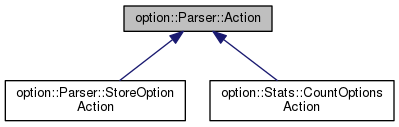
\includegraphics[width=350pt]{structoption_1_1Parser_1_1Action__inherit__graph}
\end{center}
\end{figure}
\subsection*{Public Member Functions}
\begin{DoxyCompactItemize}
\item 
virtual bool \hyperlink{structoption_1_1Parser_1_1Action_a176b5f783bb35eb015b6d2c09422457d}{perform} (\hyperlink{classoption_1_1Option}{Option} \&)
\begin{DoxyCompactList}\small\item\em Called by Parser\+::workhorse() for each \hyperlink{classoption_1_1Option}{Option} that has been successfully parsed (including unknown options if they have a \hyperlink{structoption_1_1Descriptor}{Descriptor} whose \hyperlink{structoption_1_1Descriptor_aa5d675dba0214a4abd73007ff163cc67}{Descriptor\+::check\+\_\+arg} does not return \hyperlink{namespaceoption_aee8c76a07877335762631491e7a5a1a9a9528e32563b795bd2930b12d0a5e382d}{A\+R\+G\+\_\+\+I\+L\+L\+E\+G\+AL}. \end{DoxyCompactList}\item 
virtual bool \hyperlink{structoption_1_1Parser_1_1Action_a3ec558b51e34d33d116f14587289e032}{finished} (int numargs, const char $\ast$$\ast$args)
\begin{DoxyCompactList}\small\item\em Called by Parser\+::workhorse() after finishing the parse. \end{DoxyCompactList}\end{DoxyCompactItemize}


\subsection{Member Function Documentation}
\index{option\+::\+Parser\+::\+Action@{option\+::\+Parser\+::\+Action}!finished@{finished}}
\index{finished@{finished}!option\+::\+Parser\+::\+Action@{option\+::\+Parser\+::\+Action}}
\subsubsection[{\texorpdfstring{finished(int numargs, const char $\ast$$\ast$args)}{finished(int numargs, const char **args)}}]{\setlength{\rightskip}{0pt plus 5cm}virtual bool option\+::\+Parser\+::\+Action\+::finished (
\begin{DoxyParamCaption}
\item[{int}]{numargs, }
\item[{const char $\ast$$\ast$}]{args}
\end{DoxyParamCaption}
)\hspace{0.3cm}{\ttfamily [inline]}, {\ttfamily [virtual]}}\hypertarget{structoption_1_1Parser_1_1Action_a3ec558b51e34d33d116f14587289e032}{}\label{structoption_1_1Parser_1_1Action_a3ec558b51e34d33d116f14587289e032}


Called by Parser\+::workhorse() after finishing the parse. 


\begin{DoxyParams}{Parameters}
{\em numargs} & the number of non-\/option arguments remaining \\
\hline
{\em args} & pointer to the first remaining non-\/option argument (if numargs $>$ 0).\\
\hline
\end{DoxyParams}
\begin{DoxyReturn}{Returns}
{\ttfamily false} iff a fatal error has occurred. 
\end{DoxyReturn}


Reimplemented in \hyperlink{classoption_1_1Parser_1_1StoreOptionAction_a617f675ef50a72ae36ce91f065bc8441}{option\+::\+Parser\+::\+Store\+Option\+Action}.

\index{option\+::\+Parser\+::\+Action@{option\+::\+Parser\+::\+Action}!perform@{perform}}
\index{perform@{perform}!option\+::\+Parser\+::\+Action@{option\+::\+Parser\+::\+Action}}
\subsubsection[{\texorpdfstring{perform(\+Option \&)}{perform(Option &)}}]{\setlength{\rightskip}{0pt plus 5cm}virtual bool option\+::\+Parser\+::\+Action\+::perform (
\begin{DoxyParamCaption}
\item[{{\bf Option} \&}]{}
\end{DoxyParamCaption}
)\hspace{0.3cm}{\ttfamily [inline]}, {\ttfamily [virtual]}}\hypertarget{structoption_1_1Parser_1_1Action_a176b5f783bb35eb015b6d2c09422457d}{}\label{structoption_1_1Parser_1_1Action_a176b5f783bb35eb015b6d2c09422457d}


Called by Parser\+::workhorse() for each \hyperlink{classoption_1_1Option}{Option} that has been successfully parsed (including unknown options if they have a \hyperlink{structoption_1_1Descriptor}{Descriptor} whose \hyperlink{structoption_1_1Descriptor_aa5d675dba0214a4abd73007ff163cc67}{Descriptor\+::check\+\_\+arg} does not return \hyperlink{namespaceoption_aee8c76a07877335762631491e7a5a1a9a9528e32563b795bd2930b12d0a5e382d}{A\+R\+G\+\_\+\+I\+L\+L\+E\+G\+AL}. 

Returns {\ttfamily false} iff a fatal error has occured and the parse should be aborted. 

Reimplemented in \hyperlink{classoption_1_1Parser_1_1StoreOptionAction_a8931919fba5516377c202920db2b2f84}{option\+::\+Parser\+::\+Store\+Option\+Action}, and \hyperlink{classoption_1_1Stats_1_1CountOptionsAction_a29ab8a68d0a30736b99b4d2e5dece489}{option\+::\+Stats\+::\+Count\+Options\+Action}.



The documentation for this struct was generated from the following file\+:\begin{DoxyCompactItemize}
\item 
\hyperlink{optionparser_8h}{optionparser.\+h}\end{DoxyCompactItemize}

\hypertarget{classhebi_1_1Command_1_1Actuator}{}\section{hebi\+:\+:Command\+:\+:Actuator Class Reference}
\label{classhebi_1_1Command_1_1Actuator}\index{hebi\+::\+Command\+::\+Actuator@{hebi\+::\+Command\+::\+Actuator}}


Actuator-\/specific commands.  




{\ttfamily \#include $<$command.\+hpp$>$}

\subsection*{Public Member Functions}
\begin{DoxyCompactItemize}
\item 
{\bfseries Actuator} (Hebi\+Command\+Ptr internal)\hypertarget{classhebi_1_1Command_1_1Actuator_afe321b7e8cee804d45241b64a26fe05d}{}\label{classhebi_1_1Command_1_1Actuator_afe321b7e8cee804d45241b64a26fe05d}

\item 
\hyperlink{classhebi_1_1Command_1_1FloatField}{Float\+Field} \& \hyperlink{classhebi_1_1Command_1_1Actuator_a9f9a807011bd53ba8bc9077fc6da36c6}{velocity} ()\hypertarget{classhebi_1_1Command_1_1Actuator_a9f9a807011bd53ba8bc9077fc6da36c6}{}\label{classhebi_1_1Command_1_1Actuator_a9f9a807011bd53ba8bc9077fc6da36c6}

\begin{DoxyCompactList}\small\item\em Velocity of the module output (post-\/spring), in radians/second. \end{DoxyCompactList}\item 
\hyperlink{classhebi_1_1Command_1_1FloatField}{Float\+Field} \& \hyperlink{classhebi_1_1Command_1_1Actuator_aff547c7a88a7cfa613bdbd03ed19bbdd}{torque} ()\hypertarget{classhebi_1_1Command_1_1Actuator_aff547c7a88a7cfa613bdbd03ed19bbdd}{}\label{classhebi_1_1Command_1_1Actuator_aff547c7a88a7cfa613bdbd03ed19bbdd}

\begin{DoxyCompactList}\small\item\em Torque at the module output, in N $\ast$ m. \end{DoxyCompactList}\item 
\hyperlink{classhebi_1_1Command_1_1HighResAngleField}{High\+Res\+Angle\+Field} \& \hyperlink{classhebi_1_1Command_1_1Actuator_a8ef2c47dd77981bed74b580b5832489e}{position} ()\hypertarget{classhebi_1_1Command_1_1Actuator_a8ef2c47dd77981bed74b580b5832489e}{}\label{classhebi_1_1Command_1_1Actuator_a8ef2c47dd77981bed74b580b5832489e}

\begin{DoxyCompactList}\small\item\em Position of the module output (post-\/spring), in radians. \end{DoxyCompactList}\end{DoxyCompactItemize}


\subsection{Detailed Description}
Actuator-\/specific commands. 

The documentation for this class was generated from the following file\+:\begin{DoxyCompactItemize}
\item 
command.\+hpp\end{DoxyCompactItemize}

\hypertarget{classhebi_1_1Info_1_1Settings_1_1Actuator}{}\section{hebi\+:\+:Info\+:\+:Settings\+:\+:Actuator Class Reference}
\label{classhebi_1_1Info_1_1Settings_1_1Actuator}\index{hebi\+::\+Info\+::\+Settings\+::\+Actuator@{hebi\+::\+Info\+::\+Settings\+::\+Actuator}}


Actuator-\/specific settings, such as controller gains.  




{\ttfamily \#include $<$info.\+hpp$>$}

\subsection*{Classes}
\begin{DoxyCompactItemize}
\item 
class \hyperlink{classhebi_1_1Info_1_1Settings_1_1Actuator_1_1PositionGains}{Position\+Gains}
\begin{DoxyCompactList}\small\item\em Controller gains for the position P\+ID loop. \end{DoxyCompactList}\item 
class \hyperlink{classhebi_1_1Info_1_1Settings_1_1Actuator_1_1TorqueGains}{Torque\+Gains}
\begin{DoxyCompactList}\small\item\em Controller gains for the torque P\+ID loop. \end{DoxyCompactList}\item 
class \hyperlink{classhebi_1_1Info_1_1Settings_1_1Actuator_1_1VelocityGains}{Velocity\+Gains}
\begin{DoxyCompactList}\small\item\em Controller gains for the velocity P\+ID loop. \end{DoxyCompactList}\end{DoxyCompactItemize}
\subsection*{Public Member Functions}
\begin{DoxyCompactItemize}
\item 
{\bfseries Actuator} (Hebi\+Info\+Ptr internal)\hypertarget{classhebi_1_1Info_1_1Settings_1_1Actuator_aa98fabf49405d502cb618168a1a3ab9d}{}\label{classhebi_1_1Info_1_1Settings_1_1Actuator_aa98fabf49405d502cb618168a1a3ab9d}

\item 
const \hyperlink{classhebi_1_1Info_1_1Settings_1_1Actuator_1_1PositionGains}{Position\+Gains} \& \hyperlink{classhebi_1_1Info_1_1Settings_1_1Actuator_af12d2c0a6bf954420419656002c2707e}{position\+Gains} () const \hypertarget{classhebi_1_1Info_1_1Settings_1_1Actuator_af12d2c0a6bf954420419656002c2707e}{}\label{classhebi_1_1Info_1_1Settings_1_1Actuator_af12d2c0a6bf954420419656002c2707e}

\begin{DoxyCompactList}\small\item\em Controller gains for the position P\+ID loop. \end{DoxyCompactList}\item 
const \hyperlink{classhebi_1_1Info_1_1Settings_1_1Actuator_1_1VelocityGains}{Velocity\+Gains} \& \hyperlink{classhebi_1_1Info_1_1Settings_1_1Actuator_aa125c9d85ccecd4316f400b0596bac83}{velocity\+Gains} () const \hypertarget{classhebi_1_1Info_1_1Settings_1_1Actuator_aa125c9d85ccecd4316f400b0596bac83}{}\label{classhebi_1_1Info_1_1Settings_1_1Actuator_aa125c9d85ccecd4316f400b0596bac83}

\begin{DoxyCompactList}\small\item\em Controller gains for the velocity P\+ID loop. \end{DoxyCompactList}\item 
const \hyperlink{classhebi_1_1Info_1_1Settings_1_1Actuator_1_1TorqueGains}{Torque\+Gains} \& \hyperlink{classhebi_1_1Info_1_1Settings_1_1Actuator_a02e5a290d735e150b84a4d33564891bf}{torque\+Gains} () const \hypertarget{classhebi_1_1Info_1_1Settings_1_1Actuator_a02e5a290d735e150b84a4d33564891bf}{}\label{classhebi_1_1Info_1_1Settings_1_1Actuator_a02e5a290d735e150b84a4d33564891bf}

\begin{DoxyCompactList}\small\item\em Controller gains for the torque P\+ID loop. \end{DoxyCompactList}\item 
const \hyperlink{classhebi_1_1Info_1_1FloatField}{Float\+Field} \& \hyperlink{classhebi_1_1Info_1_1Settings_1_1Actuator_a47c9c731ce9cbfe3e6b8c08f694e1cca}{spring\+Constant} () const \hypertarget{classhebi_1_1Info_1_1Settings_1_1Actuator_a47c9c731ce9cbfe3e6b8c08f694e1cca}{}\label{classhebi_1_1Info_1_1Settings_1_1Actuator_a47c9c731ce9cbfe3e6b8c08f694e1cca}

\begin{DoxyCompactList}\small\item\em The spring constant of the module. \end{DoxyCompactList}\item 
const \hyperlink{classhebi_1_1Info_1_1EnumField}{Enum\+Field}$<$ \hyperlink{classhebi_1_1Info_a154026587295ad17a3e1460f32dab668}{Control\+Strategy} $>$ \& \hyperlink{classhebi_1_1Info_1_1Settings_1_1Actuator_aaa17c720329614ca2c15083645ed9037}{control\+Strategy} () const \hypertarget{classhebi_1_1Info_1_1Settings_1_1Actuator_aaa17c720329614ca2c15083645ed9037}{}\label{classhebi_1_1Info_1_1Settings_1_1Actuator_aaa17c720329614ca2c15083645ed9037}

\begin{DoxyCompactList}\small\item\em How the position, velocity, and torque P\+ID loops are connected in order to control motor P\+WM. \end{DoxyCompactList}\end{DoxyCompactItemize}


\subsection{Detailed Description}
Actuator-\/specific settings, such as controller gains. 

The documentation for this class was generated from the following file\+:\begin{DoxyCompactItemize}
\item 
info.\+hpp\end{DoxyCompactItemize}

\hypertarget{classhebi_1_1Command_1_1Settings_1_1Actuator}{}\section{hebi\+:\+:Command\+:\+:Settings\+:\+:Actuator Class Reference}
\label{classhebi_1_1Command_1_1Settings_1_1Actuator}\index{hebi\+::\+Command\+::\+Settings\+::\+Actuator@{hebi\+::\+Command\+::\+Settings\+::\+Actuator}}


Actuator-\/specific settings, such as controller gains.  




{\ttfamily \#include $<$command.\+hpp$>$}

\subsection*{Classes}
\begin{DoxyCompactItemize}
\item 
class \hyperlink{classhebi_1_1Command_1_1Settings_1_1Actuator_1_1PositionGains}{Position\+Gains}
\begin{DoxyCompactList}\small\item\em Controller gains for the position P\+ID loop. \end{DoxyCompactList}\item 
class \hyperlink{classhebi_1_1Command_1_1Settings_1_1Actuator_1_1TorqueGains}{Torque\+Gains}
\begin{DoxyCompactList}\small\item\em Controller gains for the torque P\+ID loop. \end{DoxyCompactList}\item 
class \hyperlink{classhebi_1_1Command_1_1Settings_1_1Actuator_1_1VelocityGains}{Velocity\+Gains}
\begin{DoxyCompactList}\small\item\em Controller gains for the velocity P\+ID loop. \end{DoxyCompactList}\end{DoxyCompactItemize}
\subsection*{Public Member Functions}
\begin{DoxyCompactItemize}
\item 
{\bfseries Actuator} (Hebi\+Command\+Ptr internal)\hypertarget{classhebi_1_1Command_1_1Settings_1_1Actuator_ae1f7d2252f3eab33c549b8b646dba3f2}{}\label{classhebi_1_1Command_1_1Settings_1_1Actuator_ae1f7d2252f3eab33c549b8b646dba3f2}

\item 
\hyperlink{classhebi_1_1Command_1_1Settings_1_1Actuator_1_1PositionGains}{Position\+Gains} \& \hyperlink{classhebi_1_1Command_1_1Settings_1_1Actuator_a6cb60e0dd2f29ed1a304a2581ed2d9fa}{position\+Gains} ()\hypertarget{classhebi_1_1Command_1_1Settings_1_1Actuator_a6cb60e0dd2f29ed1a304a2581ed2d9fa}{}\label{classhebi_1_1Command_1_1Settings_1_1Actuator_a6cb60e0dd2f29ed1a304a2581ed2d9fa}

\begin{DoxyCompactList}\small\item\em Controller gains for the position P\+ID loop. \end{DoxyCompactList}\item 
\hyperlink{classhebi_1_1Command_1_1Settings_1_1Actuator_1_1VelocityGains}{Velocity\+Gains} \& \hyperlink{classhebi_1_1Command_1_1Settings_1_1Actuator_a917deb6fba9cc3190ad083b14976b33a}{velocity\+Gains} ()\hypertarget{classhebi_1_1Command_1_1Settings_1_1Actuator_a917deb6fba9cc3190ad083b14976b33a}{}\label{classhebi_1_1Command_1_1Settings_1_1Actuator_a917deb6fba9cc3190ad083b14976b33a}

\begin{DoxyCompactList}\small\item\em Controller gains for the velocity P\+ID loop. \end{DoxyCompactList}\item 
\hyperlink{classhebi_1_1Command_1_1Settings_1_1Actuator_1_1TorqueGains}{Torque\+Gains} \& \hyperlink{classhebi_1_1Command_1_1Settings_1_1Actuator_ab4986c704b655dcb9ebd2905979b66c8}{torque\+Gains} ()\hypertarget{classhebi_1_1Command_1_1Settings_1_1Actuator_ab4986c704b655dcb9ebd2905979b66c8}{}\label{classhebi_1_1Command_1_1Settings_1_1Actuator_ab4986c704b655dcb9ebd2905979b66c8}

\begin{DoxyCompactList}\small\item\em Controller gains for the torque P\+ID loop. \end{DoxyCompactList}\item 
\hyperlink{classhebi_1_1Command_1_1FloatField}{Float\+Field} \& \hyperlink{classhebi_1_1Command_1_1Settings_1_1Actuator_a6c88ef0c359b4e07a712e9aa32ff75c0}{spring\+Constant} ()\hypertarget{classhebi_1_1Command_1_1Settings_1_1Actuator_a6c88ef0c359b4e07a712e9aa32ff75c0}{}\label{classhebi_1_1Command_1_1Settings_1_1Actuator_a6c88ef0c359b4e07a712e9aa32ff75c0}

\begin{DoxyCompactList}\small\item\em The spring constant of the module. \end{DoxyCompactList}\item 
\hyperlink{classhebi_1_1Command_1_1EnumField}{Enum\+Field}$<$ \hyperlink{classhebi_1_1Command_a0f4b41003c36dee21578caddb605c64a}{Control\+Strategy} $>$ \& \hyperlink{classhebi_1_1Command_1_1Settings_1_1Actuator_a7c08db380c5c7920255626de10bdca6d}{control\+Strategy} ()\hypertarget{classhebi_1_1Command_1_1Settings_1_1Actuator_a7c08db380c5c7920255626de10bdca6d}{}\label{classhebi_1_1Command_1_1Settings_1_1Actuator_a7c08db380c5c7920255626de10bdca6d}

\begin{DoxyCompactList}\small\item\em How the position, velocity, and torque P\+ID loops are connected in order to control motor P\+WM. \end{DoxyCompactList}\end{DoxyCompactItemize}


\subsection{Detailed Description}
Actuator-\/specific settings, such as controller gains. 

The documentation for this class was generated from the following file\+:\begin{DoxyCompactItemize}
\item 
command.\+hpp\end{DoxyCompactItemize}

\hypertarget{classhebi_1_1Feedback_1_1Actuator}{}\section{hebi\+:\+:Feedback\+:\+:Actuator Class Reference}
\label{classhebi_1_1Feedback_1_1Actuator}\index{hebi\+::\+Feedback\+::\+Actuator@{hebi\+::\+Feedback\+::\+Actuator}}


Actuator-\/specific feedback.  




{\ttfamily \#include $<$feedback.\+hpp$>$}

\subsection*{Public Member Functions}
\begin{DoxyCompactItemize}
\item 
\mbox{\Hypertarget{classhebi_1_1Feedback_1_1Actuator_a2af3d7a0d6291196a10c08fe707f0c09}\label{classhebi_1_1Feedback_1_1Actuator_a2af3d7a0d6291196a10c08fe707f0c09}} 
{\bfseries Actuator} (Hebi\+Feedback\+Ptr internal)
\item 
\mbox{\Hypertarget{classhebi_1_1Feedback_1_1Actuator_aa74b5d7bcd1df8944f00058d727bf466}\label{classhebi_1_1Feedback_1_1Actuator_aa74b5d7bcd1df8944f00058d727bf466}} 
const \hyperlink{classhebi_1_1Feedback_1_1FloatField}{Float\+Field} \& \hyperlink{classhebi_1_1Feedback_1_1Actuator_aa74b5d7bcd1df8944f00058d727bf466}{velocity} () const
\begin{DoxyCompactList}\small\item\em Velocity of the module output (post-\/spring), in radians/second. \end{DoxyCompactList}\item 
\mbox{\Hypertarget{classhebi_1_1Feedback_1_1Actuator_a353436ed451bd22a34f6d42053a64b6a}\label{classhebi_1_1Feedback_1_1Actuator_a353436ed451bd22a34f6d42053a64b6a}} 
const \hyperlink{classhebi_1_1Feedback_1_1FloatField}{Float\+Field} \& \hyperlink{classhebi_1_1Feedback_1_1Actuator_a353436ed451bd22a34f6d42053a64b6a}{torque} () const
\begin{DoxyCompactList}\small\item\em Torque at the module output, in N $\ast$ m. \end{DoxyCompactList}\item 
\mbox{\Hypertarget{classhebi_1_1Feedback_1_1Actuator_a48358540dc0da8e30638267897076a00}\label{classhebi_1_1Feedback_1_1Actuator_a48358540dc0da8e30638267897076a00}} 
const \hyperlink{classhebi_1_1Feedback_1_1FloatField}{Float\+Field} \& \hyperlink{classhebi_1_1Feedback_1_1Actuator_a48358540dc0da8e30638267897076a00}{velocity\+Command} () const
\begin{DoxyCompactList}\small\item\em Commanded velocity of the module output (post-\/spring), in radians/second. \end{DoxyCompactList}\item 
\mbox{\Hypertarget{classhebi_1_1Feedback_1_1Actuator_aa9c6d12fd9f70f6038dc06bd901f00b2}\label{classhebi_1_1Feedback_1_1Actuator_aa9c6d12fd9f70f6038dc06bd901f00b2}} 
const \hyperlink{classhebi_1_1Feedback_1_1FloatField}{Float\+Field} \& \hyperlink{classhebi_1_1Feedback_1_1Actuator_aa9c6d12fd9f70f6038dc06bd901f00b2}{torque\+Command} () const
\begin{DoxyCompactList}\small\item\em Commanded torque at the module output, in N $\ast$ m. \end{DoxyCompactList}\item 
\mbox{\Hypertarget{classhebi_1_1Feedback_1_1Actuator_a3713e0a4cf660f2fa8729e2298867c14}\label{classhebi_1_1Feedback_1_1Actuator_a3713e0a4cf660f2fa8729e2298867c14}} 
const \hyperlink{classhebi_1_1Feedback_1_1FloatField}{Float\+Field} \& \hyperlink{classhebi_1_1Feedback_1_1Actuator_a3713e0a4cf660f2fa8729e2298867c14}{deflection} () const
\begin{DoxyCompactList}\small\item\em Difference (in radians) between the pre-\/spring and post-\/spring output position. \end{DoxyCompactList}\item 
\mbox{\Hypertarget{classhebi_1_1Feedback_1_1Actuator_a69dcfd58ff4afa1a777dd372adaf632b}\label{classhebi_1_1Feedback_1_1Actuator_a69dcfd58ff4afa1a777dd372adaf632b}} 
const \hyperlink{classhebi_1_1Feedback_1_1FloatField}{Float\+Field} \& \hyperlink{classhebi_1_1Feedback_1_1Actuator_a69dcfd58ff4afa1a777dd372adaf632b}{deflection\+Velocity} () const
\begin{DoxyCompactList}\small\item\em Velocity (in radians/second) of the difference between the pre-\/spring and post-\/spring output position. \end{DoxyCompactList}\item 
\mbox{\Hypertarget{classhebi_1_1Feedback_1_1Actuator_ad4e745235c1ccc801f06c359843247de}\label{classhebi_1_1Feedback_1_1Actuator_ad4e745235c1ccc801f06c359843247de}} 
const \hyperlink{classhebi_1_1Feedback_1_1FloatField}{Float\+Field} \& \hyperlink{classhebi_1_1Feedback_1_1Actuator_ad4e745235c1ccc801f06c359843247de}{motor\+Velocity} () const
\begin{DoxyCompactList}\small\item\em The velocity (in radians/second) of the motor shaft. \end{DoxyCompactList}\item 
\mbox{\Hypertarget{classhebi_1_1Feedback_1_1Actuator_ab484c2d8f437e5bf3693b1353f23f849}\label{classhebi_1_1Feedback_1_1Actuator_ab484c2d8f437e5bf3693b1353f23f849}} 
const \hyperlink{classhebi_1_1Feedback_1_1FloatField}{Float\+Field} \& \hyperlink{classhebi_1_1Feedback_1_1Actuator_ab484c2d8f437e5bf3693b1353f23f849}{motor\+Current} () const
\begin{DoxyCompactList}\small\item\em Current supplied to the motor. \end{DoxyCompactList}\item 
\mbox{\Hypertarget{classhebi_1_1Feedback_1_1Actuator_a68d8af73c19649d720e35b378b11df99}\label{classhebi_1_1Feedback_1_1Actuator_a68d8af73c19649d720e35b378b11df99}} 
const \hyperlink{classhebi_1_1Feedback_1_1FloatField}{Float\+Field} \& \hyperlink{classhebi_1_1Feedback_1_1Actuator_a68d8af73c19649d720e35b378b11df99}{motor\+Sensor\+Temperature} () const
\begin{DoxyCompactList}\small\item\em The temperature from a sensor near the motor housing. \end{DoxyCompactList}\item 
\mbox{\Hypertarget{classhebi_1_1Feedback_1_1Actuator_a586c2e23d1ed355bff2eece3fcd54118}\label{classhebi_1_1Feedback_1_1Actuator_a586c2e23d1ed355bff2eece3fcd54118}} 
const \hyperlink{classhebi_1_1Feedback_1_1FloatField}{Float\+Field} \& \hyperlink{classhebi_1_1Feedback_1_1Actuator_a586c2e23d1ed355bff2eece3fcd54118}{motor\+Winding\+Current} () const
\begin{DoxyCompactList}\small\item\em The estimated current in the motor windings. \end{DoxyCompactList}\item 
\mbox{\Hypertarget{classhebi_1_1Feedback_1_1Actuator_ac03a9d30d23d30dc066688cf269a0a3f}\label{classhebi_1_1Feedback_1_1Actuator_ac03a9d30d23d30dc066688cf269a0a3f}} 
const \hyperlink{classhebi_1_1Feedback_1_1FloatField}{Float\+Field} \& \hyperlink{classhebi_1_1Feedback_1_1Actuator_ac03a9d30d23d30dc066688cf269a0a3f}{motor\+Winding\+Temperature} () const
\begin{DoxyCompactList}\small\item\em The estimated temperature of the motor windings. \end{DoxyCompactList}\item 
\mbox{\Hypertarget{classhebi_1_1Feedback_1_1Actuator_a3b92ce1c90558e9b6f80f82a9be45e3c}\label{classhebi_1_1Feedback_1_1Actuator_a3b92ce1c90558e9b6f80f82a9be45e3c}} 
const \hyperlink{classhebi_1_1Feedback_1_1FloatField}{Float\+Field} \& \hyperlink{classhebi_1_1Feedback_1_1Actuator_a3b92ce1c90558e9b6f80f82a9be45e3c}{motor\+Housing\+Temperature} () const
\begin{DoxyCompactList}\small\item\em The estimated temperature of the motor housing. \end{DoxyCompactList}\item 
\mbox{\Hypertarget{classhebi_1_1Feedback_1_1Actuator_a960ff09a3a8a57188e6e7ca9435d9fba}\label{classhebi_1_1Feedback_1_1Actuator_a960ff09a3a8a57188e6e7ca9435d9fba}} 
const \hyperlink{classhebi_1_1Feedback_1_1HighResAngleField}{High\+Res\+Angle\+Field} \& \hyperlink{classhebi_1_1Feedback_1_1Actuator_a960ff09a3a8a57188e6e7ca9435d9fba}{position} () const
\begin{DoxyCompactList}\small\item\em Position of the module output (post-\/spring), in radians. \end{DoxyCompactList}\item 
\mbox{\Hypertarget{classhebi_1_1Feedback_1_1Actuator_ac52ee60b21c703a81c918157ee87b8e4}\label{classhebi_1_1Feedback_1_1Actuator_ac52ee60b21c703a81c918157ee87b8e4}} 
const \hyperlink{classhebi_1_1Feedback_1_1HighResAngleField}{High\+Res\+Angle\+Field} \& \hyperlink{classhebi_1_1Feedback_1_1Actuator_ac52ee60b21c703a81c918157ee87b8e4}{position\+Command} () const
\begin{DoxyCompactList}\small\item\em Commanded position of the module output (post-\/spring), in radians. \end{DoxyCompactList}\end{DoxyCompactItemize}


\subsection{Detailed Description}
Actuator-\/specific feedback. 

The documentation for this class was generated from the following file\+:\begin{DoxyCompactItemize}
\item 
feedback.\+hpp\end{DoxyCompactItemize}

\hypertarget{structArg}{}\section{Arg Struct Reference}
\label{structArg}\index{Arg@{Arg}}


Inheritance diagram for Arg\+:\nopagebreak
\begin{figure}[H]
\begin{center}
\leavevmode
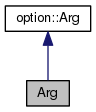
\includegraphics[width=144pt]{structArg__inherit__graph}
\end{center}
\end{figure}


Collaboration diagram for Arg\+:\nopagebreak
\begin{figure}[H]
\begin{center}
\leavevmode
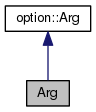
\includegraphics[width=144pt]{structArg__coll__graph}
\end{center}
\end{figure}
\subsection*{Static Public Member Functions}
\begin{DoxyCompactItemize}
\item 
\mbox{\Hypertarget{structArg_ac02bc8cf3aec0a37643d1c4e72e53247}\label{structArg_ac02bc8cf3aec0a37643d1c4e72e53247}} 
static void {\bfseries print\+Error} (const char $\ast$msg1, const \hyperlink{classoption_1_1Option}{option\+::\+Option} \&opt, const char $\ast$msg2)
\item 
\mbox{\Hypertarget{structArg_a27e735e03504971f760309d1045b2602}\label{structArg_a27e735e03504971f760309d1045b2602}} 
static \hyperlink{namespaceoption_aee8c76a07877335762631491e7a5a1a9}{option\+::\+Arg\+Status} {\bfseries Unknown} (const \hyperlink{classoption_1_1Option}{option\+::\+Option} \&option, bool msg)
\item 
\mbox{\Hypertarget{structArg_a16fdbf5d402df5a97db981654b16841e}\label{structArg_a16fdbf5d402df5a97db981654b16841e}} 
static \hyperlink{namespaceoption_aee8c76a07877335762631491e7a5a1a9}{option\+::\+Arg\+Status} {\bfseries Pair} (const \hyperlink{classoption_1_1Option}{option\+::\+Option} \&option, bool msg)
\item 
\mbox{\Hypertarget{structArg_ae9e0da122154013b1f7b6c0613a99c5c}\label{structArg_ae9e0da122154013b1f7b6c0613a99c5c}} 
static \hyperlink{namespaceoption_aee8c76a07877335762631491e7a5a1a9}{option\+::\+Arg\+Status} {\bfseries Mac} (const \hyperlink{classoption_1_1Option}{option\+::\+Option} \&option, bool msg)
\item 
\mbox{\Hypertarget{structArg_a44445181427d8c2b953ed1ac8cf653f0}\label{structArg_a44445181427d8c2b953ed1ac8cf653f0}} 
static \hyperlink{namespaceoption_aee8c76a07877335762631491e7a5a1a9}{option\+::\+Arg\+Status} {\bfseries Non\+Empty} (const \hyperlink{classoption_1_1Option}{option\+::\+Option} \&option, bool msg)
\end{DoxyCompactItemize}


The documentation for this struct was generated from the following file\+:\begin{DoxyCompactItemize}
\item 
\hyperlink{lookup__helpers_8cpp}{lookup\+\_\+helpers.\+cpp}\end{DoxyCompactItemize}

\hypertarget{structoption_1_1Arg}{}\section{option\+:\+:Arg Struct Reference}
\label{structoption_1_1Arg}\index{option\+::\+Arg@{option\+::\+Arg}}


Functions for checking the validity of option arguments.  




{\ttfamily \#include $<$optionparser.\+h$>$}



Inheritance diagram for option\+:\+:Arg\+:\nopagebreak
\begin{figure}[H]
\begin{center}
\leavevmode
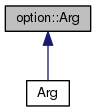
\includegraphics[width=144pt]{structoption_1_1Arg__inherit__graph}
\end{center}
\end{figure}
\subsection*{Static Public Member Functions}
\begin{DoxyCompactItemize}
\item 
static \hyperlink{namespaceoption_aee8c76a07877335762631491e7a5a1a9}{Arg\+Status} \hyperlink{structoption_1_1Arg_a7fc01987899c91c6b6a1be5711a46e22}{None} (const \hyperlink{classoption_1_1Option}{Option} \&, bool)\hypertarget{structoption_1_1Arg_a7fc01987899c91c6b6a1be5711a46e22}{}\label{structoption_1_1Arg_a7fc01987899c91c6b6a1be5711a46e22}

\begin{DoxyCompactList}\small\item\em For options that don\textquotesingle{}t take an argument\+: Returns A\+R\+G\+\_\+\+N\+O\+NE. \end{DoxyCompactList}\item 
static \hyperlink{namespaceoption_aee8c76a07877335762631491e7a5a1a9}{Arg\+Status} \hyperlink{structoption_1_1Arg_aadb5316ecbc9eb0a7f0019d14bf35ad0}{Optional} (const \hyperlink{classoption_1_1Option}{Option} \&option, bool)\hypertarget{structoption_1_1Arg_aadb5316ecbc9eb0a7f0019d14bf35ad0}{}\label{structoption_1_1Arg_aadb5316ecbc9eb0a7f0019d14bf35ad0}

\begin{DoxyCompactList}\small\item\em Returns A\+R\+G\+\_\+\+OK if the argument is attached and A\+R\+G\+\_\+\+I\+G\+N\+O\+RE otherwise. \end{DoxyCompactList}\end{DoxyCompactItemize}


\subsection{Detailed Description}
Functions for checking the validity of option arguments. 

Every \hyperlink{classoption_1_1Option}{Option} has such a function assigned in its \hyperlink{structoption_1_1Descriptor}{Descriptor}. 
\begin{DoxyCode}
Descriptor usage[] = \{ \{UNKNOWN, 0, \textcolor{stringliteral}{""}, \textcolor{stringliteral}{""}, \hyperlink{structoption_1_1Arg_a7fc01987899c91c6b6a1be5711a46e22}{Arg::None}, \textcolor{stringliteral}{""}\}, ... \};
\end{DoxyCode}


A Check\+Arg function has the following signature\+: 
\begin{DoxyCode}
\hyperlink{namespaceoption_aee8c76a07877335762631491e7a5a1a9}{ArgStatus} \hyperlink{namespaceoption_a4cdf403efae65e18bf850e2001b12a2a}{CheckArg}(\textcolor{keyword}{const} Option& option, \textcolor{keywordtype}{bool} msg); 
\end{DoxyCode}


It is used to check if a potential argument would be acceptable for the option. It will even be called if there is no argument. In that case {\ttfamily option.\+arg} will be {\ttfamily N\+U\+LL}.

If {\ttfamily msg} is {\ttfamily true} and the function determines that an argument is not acceptable and that this is a fatal error, it should output a message to the user before returning \hyperlink{namespaceoption_aee8c76a07877335762631491e7a5a1a9a9528e32563b795bd2930b12d0a5e382d}{A\+R\+G\+\_\+\+I\+L\+L\+E\+G\+AL}. If {\ttfamily msg} is {\ttfamily false} the function should remain silent (or you will get duplicate messages).

See \hyperlink{namespaceoption_aee8c76a07877335762631491e7a5a1a9}{Arg\+Status} for the meaning of the return values.

While you can provide your own functions, often the following pre-\/defined checks (which never return \hyperlink{namespaceoption_aee8c76a07877335762631491e7a5a1a9a9528e32563b795bd2930b12d0a5e382d}{A\+R\+G\+\_\+\+I\+L\+L\+E\+G\+AL}) will suffice\+:

\begin{DoxyItemize}
\item {\ttfamily \hyperlink{structoption_1_1Arg_a7fc01987899c91c6b6a1be5711a46e22}{Arg\+::\+None}} For options that don\textquotesingle{}t take an argument\+: Returns A\+R\+G\+\_\+\+N\+O\+NE. \item {\ttfamily \hyperlink{structoption_1_1Arg_aadb5316ecbc9eb0a7f0019d14bf35ad0}{Arg\+::\+Optional}} Returns A\+R\+G\+\_\+\+OK if the argument is attached and A\+R\+G\+\_\+\+I\+G\+N\+O\+RE otherwise.\end{DoxyItemize}
The following example code can serve as starting place for writing your own more complex Check\+Arg functions\+: 
\begin{DoxyCode}
\textcolor{keyword}{struct }\hyperlink{structArg}{Arg}: \textcolor{keyword}{public} \hyperlink{structoption_1_1Arg}{option::Arg}
\{
  \textcolor{keyword}{static} \textcolor{keywordtype}{void} printError(\textcolor{keyword}{const} \textcolor{keywordtype}{char}* msg1, \textcolor{keyword}{const} \hyperlink{classoption_1_1Option}{option::Option}& opt, \textcolor{keyword}{const} \textcolor{keywordtype}{char}* msg2)
  \{
    fprintf(stderr, \textcolor{stringliteral}{"ERROR: %s"}, msg1);
    fwrite(opt.\hyperlink{classoption_1_1Option_a02a76b4896abd22d0ba8514362261de9}{name}, opt.\hyperlink{classoption_1_1Option_a3aa2957b19ad5815873441b415d56050}{namelen}, 1, stderr);
    fprintf(stderr, \textcolor{stringliteral}{"%s"}, msg2);
  \}

  \textcolor{keyword}{static} \hyperlink{namespaceoption_aee8c76a07877335762631491e7a5a1a9}{option::ArgStatus} Unknown(\textcolor{keyword}{const} \hyperlink{classoption_1_1Option}{option::Option}& option, \textcolor{keywordtype}{bool} msg)
  \{
    \textcolor{keywordflow}{if} (msg) printError(\textcolor{stringliteral}{"Unknown option '"}, option, \textcolor{stringliteral}{"'\(\backslash\)n"});
    \textcolor{keywordflow}{return} \hyperlink{namespaceoption_aee8c76a07877335762631491e7a5a1a9a9528e32563b795bd2930b12d0a5e382d}{option::ARG\_ILLEGAL};
  \}

  \textcolor{keyword}{static} \hyperlink{namespaceoption_aee8c76a07877335762631491e7a5a1a9}{option::ArgStatus} Required(\textcolor{keyword}{const} \hyperlink{classoption_1_1Option}{option::Option}& option, \textcolor{keywordtype}{bool} msg)
  \{
    \textcolor{keywordflow}{if} (option.\hyperlink{classoption_1_1Option_a402be734987458364b0f473acae36238}{arg} != 0)
      \textcolor{keywordflow}{return} \hyperlink{namespaceoption_aee8c76a07877335762631491e7a5a1a9a445e08cb1747e5a22929e7ef2da43b55}{option::ARG\_OK};

    \textcolor{keywordflow}{if} (msg) printError(\textcolor{stringliteral}{"Option '"}, option, \textcolor{stringliteral}{"' requires an argument\(\backslash\)n"});
    \textcolor{keywordflow}{return} \hyperlink{namespaceoption_aee8c76a07877335762631491e7a5a1a9a9528e32563b795bd2930b12d0a5e382d}{option::ARG\_ILLEGAL};
  \}

  \textcolor{keyword}{static} \hyperlink{namespaceoption_aee8c76a07877335762631491e7a5a1a9}{option::ArgStatus} NonEmpty(\textcolor{keyword}{const} \hyperlink{classoption_1_1Option}{option::Option}& option, \textcolor{keywordtype}{bool} msg)
  \{
    \textcolor{keywordflow}{if} (option.\hyperlink{classoption_1_1Option_a402be734987458364b0f473acae36238}{arg} != 0 && option.\hyperlink{classoption_1_1Option_a402be734987458364b0f473acae36238}{arg}[0] != 0)
      \textcolor{keywordflow}{return} \hyperlink{namespaceoption_aee8c76a07877335762631491e7a5a1a9a445e08cb1747e5a22929e7ef2da43b55}{option::ARG\_OK};

    \textcolor{keywordflow}{if} (msg) printError(\textcolor{stringliteral}{"Option '"}, option, \textcolor{stringliteral}{"' requires a non-empty argument\(\backslash\)n"});
    \textcolor{keywordflow}{return} \hyperlink{namespaceoption_aee8c76a07877335762631491e7a5a1a9a9528e32563b795bd2930b12d0a5e382d}{option::ARG\_ILLEGAL};
  \}

  \textcolor{keyword}{static} \hyperlink{namespaceoption_aee8c76a07877335762631491e7a5a1a9}{option::ArgStatus} Numeric(\textcolor{keyword}{const} \hyperlink{classoption_1_1Option}{option::Option}& option, \textcolor{keywordtype}{bool} msg)
  \{
    \textcolor{keywordtype}{char}* endptr = 0;
    \textcolor{keywordflow}{if} (option.\hyperlink{classoption_1_1Option_a402be734987458364b0f473acae36238}{arg} != 0 && strtol(option.\hyperlink{classoption_1_1Option_a402be734987458364b0f473acae36238}{arg}, &endptr, 10))\{\};
    \textcolor{keywordflow}{if} (endptr != option.\hyperlink{classoption_1_1Option_a402be734987458364b0f473acae36238}{arg} && *endptr == 0)
      \textcolor{keywordflow}{return} \hyperlink{namespaceoption_aee8c76a07877335762631491e7a5a1a9a445e08cb1747e5a22929e7ef2da43b55}{option::ARG\_OK};

    \textcolor{keywordflow}{if} (msg) printError(\textcolor{stringliteral}{"Option '"}, option, \textcolor{stringliteral}{"' requires a numeric argument\(\backslash\)n"});
    \textcolor{keywordflow}{return} \hyperlink{namespaceoption_aee8c76a07877335762631491e7a5a1a9a9528e32563b795bd2930b12d0a5e382d}{option::ARG\_ILLEGAL};
  \}
\};
\end{DoxyCode}
 

The documentation for this struct was generated from the following file\+:\begin{DoxyCompactItemize}
\item 
\hyperlink{optionparser_8h}{optionparser.\+h}\end{DoxyCompactItemize}

\hypertarget{classarmcontroller}{}\section{armcontroller Class Reference}
\label{classarmcontroller}\index{armcontroller@{armcontroller}}


Arm Controller Node for the H\+E\+BI Robotics 5-\/\+D\+OF Manipulator Arm.  


\subsection*{Public Member Functions}
\begin{DoxyCompactItemize}
\item 
\hyperlink{classarmcontroller_a7e2b5cd80851fced3e54641422fb04dd}{armcontroller} ()
\item 
void \hyperlink{classarmcontroller_a45794311f7ab89c67fe7423e07ea19d7}{init} ()
\item 
bool \hyperlink{classarmcontroller_a3cba85249ae1746aeac14d12b68becdc}{update\+Feedback} ()
\item 
void \hyperlink{classarmcontroller_af8bbda9cbee82997b7429ecda7c5412b}{get\+Feedback\+Msg} (sensor\+\_\+msgs\+::\+Joint\+State \&joint\+State\+\_\+fbk, trajectory\+\_\+msgs\+::\+Joint\+Trajectory\+Point \&trajectory\+Cmd\+\_\+fbk, model\+\_\+learning\+::\+Feedback\+ML \&armcontroller\+\_\+fbk)
\item 
void \hyperlink{classarmcontroller_ab2a040d42baac477ccc328d03b8c8903}{controller} (const Eigen\+::\+Vector\+Xd \&position\+Cmd, const Eigen\+::\+Vector\+Xd \&velocity\+Cmd, const Eigen\+::\+Vector\+Xd \&accel\+Cmd, std\+::vector$<$ double $>$ \&torque)
\item 
void \hyperlink{classarmcontroller_aa96c09e059c416f996774d4bf4b80619}{feedback\+Control} (const Eigen\+::\+Vector\+Xd \&error\+\_\+pos, const Eigen\+::\+Vector\+Xd \&error\+\_\+vel, std\+::vector$<$ double $>$ \&torque)
\item 
bool \hyperlink{classarmcontroller_aeefa5bf9839dd31ba78b33cfe092505c}{send\+Command} (const std\+::vector$<$ double $>$ \&alpha, const std\+::vector$<$ double $>$ \&torque)
\item 
bool \hyperlink{classarmcontroller_a124397944174948c82524f6632e21371}{send\+Torque\+Command} (const std\+::vector$<$ double $>$ \&torque)
\item 
void \hyperlink{classarmcontroller_ae16ff33ed407aabe5694da11807d8142}{W\+M\+A\+Filter} (const std\+::vector$<$ double $>$ \&velocity, const std\+::vector$<$ double $>$ \&motor\+Temp, std\+::vector$<$ double $>$ \&velocity\+Flt, std\+::vector$<$ double $>$ \&motor\+Temp\+Flt)
\item 
void \hyperlink{classarmcontroller_a26e78647cafc275e2c633f8e115c28c7}{moving\+Average} (const std\+::vector$<$ double $>$ \&data\+\_\+vector, const int \&num, const int \&vec\+\_\+sum, double \&W\+MA, double \&numerator, double \&total) const
\item 
void \hyperlink{classarmcontroller_a53acf57dd669cb3d2634b3d508a0d439}{subscriber\+Callback} (const model\+\_\+learning\+::\+Command\+ML \&cmd)
\item 
\mbox{\Hypertarget{classarmcontroller_a45794311f7ab89c67fe7423e07ea19d7}\label{classarmcontroller_a45794311f7ab89c67fe7423e07ea19d7}} 
void {\bfseries init} ()
\item 
\mbox{\Hypertarget{classarmcontroller_a3cba85249ae1746aeac14d12b68becdc}\label{classarmcontroller_a3cba85249ae1746aeac14d12b68becdc}} 
bool {\bfseries update\+Feedback} ()
\item 
\mbox{\Hypertarget{classarmcontroller_af1970af350bf0902f57bdbf4089f3b13}\label{classarmcontroller_af1970af350bf0902f57bdbf4089f3b13}} 
void {\bfseries get\+Feedback\+Msg} (sensor\+\_\+msgs\+::\+Joint\+State \&, trajectory\+\_\+msgs\+::\+Joint\+Trajectory\+Point \&, model\+\_\+learning\+::\+Feedback\+ML \&)
\item 
\mbox{\Hypertarget{classarmcontroller_a5d9414eb9b6c92b3f19f177c44f9f6f1}\label{classarmcontroller_a5d9414eb9b6c92b3f19f177c44f9f6f1}} 
void {\bfseries controller} (const Eigen\+::\+Vector\+Xd \&, const Eigen\+::\+Vector\+Xd \&, const Eigen\+::\+Vector\+Xd \&, std\+::vector$<$ double $>$ \&)
\item 
\mbox{\Hypertarget{classarmcontroller_a2385c8f95fd011e1206d2730615a4fad}\label{classarmcontroller_a2385c8f95fd011e1206d2730615a4fad}} 
void {\bfseries feedback\+Control} (const Eigen\+::\+Vector\+Xd \&, const Eigen\+::\+Vector\+Xd \&, std\+::vector$<$ double $>$ \&)
\item 
\mbox{\Hypertarget{classarmcontroller_a146f6d320cd7641c9fbc8c7b014a7ceb}\label{classarmcontroller_a146f6d320cd7641c9fbc8c7b014a7ceb}} 
bool {\bfseries send\+Command} (const std\+::vector$<$ double $>$ \&, const std\+::vector$<$ double $>$ \&)
\item 
\mbox{\Hypertarget{classarmcontroller_adb671e988673c3750f3c846cac593eba}\label{classarmcontroller_adb671e988673c3750f3c846cac593eba}} 
bool {\bfseries send\+Torque\+Command} (const std\+::vector$<$ double $>$ \&)
\item 
\mbox{\Hypertarget{classarmcontroller_a9f48bad4ba4c88f294d1dd78df260fc7}\label{classarmcontroller_a9f48bad4ba4c88f294d1dd78df260fc7}} 
void {\bfseries subscriber\+Callback} (const model\+\_\+learning\+::\+Command\+ML \&)
\item 
\mbox{\Hypertarget{classarmcontroller_ac707c804ed04bcbf212c3c5456f4dffe}\label{classarmcontroller_ac707c804ed04bcbf212c3c5456f4dffe}} 
void {\bfseries W\+M\+A\+Filter} (const std\+::vector$<$ double $>$ \&, const std\+::vector$<$ double $>$ \&, std\+::vector$<$ double $>$ \&, std\+::vector$<$ double $>$ \&)
\item 
\mbox{\Hypertarget{classarmcontroller_adbe2ad7337bc5ac6c31502def583ed3a}\label{classarmcontroller_adbe2ad7337bc5ac6c31502def583ed3a}} 
void {\bfseries moving\+Average} (const std\+::vector$<$ double $>$ \&, const int \&, const int \&, double \&, double \&, double \&) const
\end{DoxyCompactItemize}
\subsection*{Public Attributes}
\begin{DoxyCompactItemize}
\item 
\mbox{\Hypertarget{classarmcontroller_a874e5713e57b27d8bd2411a8489f7866}\label{classarmcontroller_a874e5713e57b27d8bd2411a8489f7866}} 
std\+::deque$<$ double $>$ {\bfseries single\+\_\+vel\+\_\+que1}
\item 
\mbox{\Hypertarget{classarmcontroller_a81cbec8fd65f32026d45d39261c0dda2}\label{classarmcontroller_a81cbec8fd65f32026d45d39261c0dda2}} 
std\+::deque$<$ double $>$ {\bfseries single\+\_\+vel\+\_\+que2}
\item 
\mbox{\Hypertarget{classarmcontroller_aec26a722458e61e1d19bb2792727ba76}\label{classarmcontroller_aec26a722458e61e1d19bb2792727ba76}} 
std\+::deque$<$ double $>$ {\bfseries single\+\_\+vel\+\_\+que3}
\item 
\mbox{\Hypertarget{classarmcontroller_af9ea47e211011bd1b1e0d99d98073e58}\label{classarmcontroller_af9ea47e211011bd1b1e0d99d98073e58}} 
std\+::deque$<$ double $>$ {\bfseries single\+\_\+vel\+\_\+que4}
\item 
\mbox{\Hypertarget{classarmcontroller_aa15c4f2ae51f44ca935c3625211155e9}\label{classarmcontroller_aa15c4f2ae51f44ca935c3625211155e9}} 
std\+::deque$<$ double $>$ {\bfseries single\+\_\+vel\+\_\+que5}
\item 
\mbox{\Hypertarget{classarmcontroller_acfb8b7af9f3b36d81b3a94559c6a2e28}\label{classarmcontroller_acfb8b7af9f3b36d81b3a94559c6a2e28}} 
std\+::deque$<$ double $>$ {\bfseries single\+\_\+temp\+\_\+que1}
\item 
\mbox{\Hypertarget{classarmcontroller_af2ade00ba55165258195ea263150cdf4}\label{classarmcontroller_af2ade00ba55165258195ea263150cdf4}} 
std\+::deque$<$ double $>$ {\bfseries single\+\_\+temp\+\_\+que2}
\item 
\mbox{\Hypertarget{classarmcontroller_a0b0fa6095474fdfd30742967f04c5825}\label{classarmcontroller_a0b0fa6095474fdfd30742967f04c5825}} 
std\+::deque$<$ double $>$ {\bfseries single\+\_\+temp\+\_\+que3}
\item 
\mbox{\Hypertarget{classarmcontroller_aad87315185a3143531b44fc88ea36bb7}\label{classarmcontroller_aad87315185a3143531b44fc88ea36bb7}} 
std\+::deque$<$ double $>$ {\bfseries single\+\_\+temp\+\_\+que4}
\item 
\mbox{\Hypertarget{classarmcontroller_a02fb1470c7f547094592fa8589d96f82}\label{classarmcontroller_a02fb1470c7f547094592fa8589d96f82}} 
std\+::deque$<$ double $>$ {\bfseries single\+\_\+temp\+\_\+que5}
\item 
\mbox{\Hypertarget{classarmcontroller_a98c171b07686d075da4c32b27e0920bd}\label{classarmcontroller_a98c171b07686d075da4c32b27e0920bd}} 
double {\bfseries last\+\_\+alpha4}
\end{DoxyCompactItemize}


\subsection{Detailed Description}
Arm Controller Node for the H\+E\+BI Robotics 5-\/\+D\+OF Manipulator Arm. 

Run the arm controller node that receives feedback from and sends commands to the H\+E\+BI modules \begin{DoxyVerb}@Author Ky Woodard\end{DoxyVerb}
 

\subsection{Constructor \& Destructor Documentation}
\mbox{\Hypertarget{classarmcontroller_a7e2b5cd80851fced3e54641422fb04dd}\label{classarmcontroller_a7e2b5cd80851fced3e54641422fb04dd}} 
\index{armcontroller@{armcontroller}!armcontroller@{armcontroller}}
\index{armcontroller@{armcontroller}!armcontroller@{armcontroller}}
\subsubsection{\texorpdfstring{armcontroller()}{armcontroller()}}
{\footnotesize\ttfamily armcontroller\+::armcontroller (\begin{DoxyParamCaption}{ }\end{DoxyParamCaption})}

Constructor for the arm controller, which initializes values used 

\subsection{Member Function Documentation}
\mbox{\Hypertarget{classarmcontroller_ab2a040d42baac477ccc328d03b8c8903}\label{classarmcontroller_ab2a040d42baac477ccc328d03b8c8903}} 
\index{armcontroller@{armcontroller}!controller@{controller}}
\index{controller@{controller}!armcontroller@{armcontroller}}
\subsubsection{\texorpdfstring{controller()}{controller()}}
{\footnotesize\ttfamily void armcontroller\+::controller (\begin{DoxyParamCaption}\item[{const Eigen\+::\+Vector\+Xd \&}]{position\+Cmd,  }\item[{const Eigen\+::\+Vector\+Xd \&}]{velocity\+Cmd,  }\item[{const Eigen\+::\+Vector\+Xd \&}]{accel\+Cmd,  }\item[{std\+::vector$<$ double $>$ \&}]{torque }\end{DoxyParamCaption})}

Generates the torque command based off the feedback and feedforward control components 
\begin{DoxyParams}[1]{Parameters}
\mbox{\tt in}  & {\em position\+Cmd} & desired joint position commands \mbox{[}rad\mbox{]} \\
\hline
\mbox{\tt in}  & {\em velocity\+Cmd} & desired joint velocity commands \mbox{[}rad/s\mbox{]} \\
\hline
\mbox{\tt in}  & {\em accel\+Cmd} & desired joint acceleration commands \mbox{[}rad/s$^\wedge$s\mbox{]} \\
\hline
\mbox{\tt out}  & {\em torque} & module input torques \mbox{[}N-\/m\mbox{]} \\
\hline
\end{DoxyParams}
\mbox{\Hypertarget{classarmcontroller_aa96c09e059c416f996774d4bf4b80619}\label{classarmcontroller_aa96c09e059c416f996774d4bf4b80619}} 
\index{armcontroller@{armcontroller}!feedback\+Control@{feedback\+Control}}
\index{feedback\+Control@{feedback\+Control}!armcontroller@{armcontroller}}
\subsubsection{\texorpdfstring{feedback\+Control()}{feedbackControl()}}
{\footnotesize\ttfamily void armcontroller\+::feedback\+Control (\begin{DoxyParamCaption}\item[{const Eigen\+::\+Vector\+Xd \&}]{error\+\_\+pos,  }\item[{const Eigen\+::\+Vector\+Xd \&}]{error\+\_\+vel,  }\item[{std\+::vector$<$ double $>$ \&}]{torque }\end{DoxyParamCaption})}

Linear feedback controller on position and velocity 
\begin{DoxyParams}[1]{Parameters}
\mbox{\tt in}  & {\em error\+\_\+pos} & joint position errors \mbox{[}rad\mbox{]} \\
\hline
\mbox{\tt in}  & {\em error\+\_\+vel} & joint velocity errors \mbox{[}rad/s\mbox{]} \\
\hline
\mbox{\tt out}  & {\em torque} & joint control torques \mbox{[}N-\/m\mbox{]} \\
\hline
\end{DoxyParams}
\mbox{\Hypertarget{classarmcontroller_af8bbda9cbee82997b7429ecda7c5412b}\label{classarmcontroller_af8bbda9cbee82997b7429ecda7c5412b}} 
\index{armcontroller@{armcontroller}!get\+Feedback\+Msg@{get\+Feedback\+Msg}}
\index{get\+Feedback\+Msg@{get\+Feedback\+Msg}!armcontroller@{armcontroller}}
\subsubsection{\texorpdfstring{get\+Feedback\+Msg()}{getFeedbackMsg()}}
{\footnotesize\ttfamily void armcontroller\+::get\+Feedback\+Msg (\begin{DoxyParamCaption}\item[{sensor\+\_\+msgs\+::\+Joint\+State \&}]{joint\+State\+\_\+fbk,  }\item[{trajectory\+\_\+msgs\+::\+Joint\+Trajectory\+Point \&}]{trajectory\+Cmd\+\_\+fbk,  }\item[{model\+\_\+learning\+::\+Feedback\+ML \&}]{armcontroller\+\_\+fbk }\end{DoxyParamCaption})}

Getter function for the feedback to pull the most recent feedback call 
\begin{DoxyParams}[1]{Parameters}
\mbox{\tt out}  & {\em joint\+State\+\_\+fbk} & R\+OS standard Joint\+State message \\
\hline
\mbox{\tt out}  & {\em trajectory\+Cmd\+\_\+fbk} & R\+OS standard Joint\+Trajectory message \\
\hline
\mbox{\tt out}  & {\em armcontroller\+\_\+fbk} & Custom message encapsilating joint\+State Joint\+Trajectory and all custom inputs \\
\hline
\end{DoxyParams}
\begin{DoxyReturn}{Returns}
flag signifying if the Feedback was update successfully 
\end{DoxyReturn}
\mbox{\Hypertarget{classarmcontroller_a45794311f7ab89c67fe7423e07ea19d7}\label{classarmcontroller_a45794311f7ab89c67fe7423e07ea19d7}} 
\index{armcontroller@{armcontroller}!init@{init}}
\index{init@{init}!armcontroller@{armcontroller}}
\subsubsection{\texorpdfstring{init()}{init()}}
{\footnotesize\ttfamily void armcontroller\+::init (\begin{DoxyParamCaption}{ }\end{DoxyParamCaption})}

Initialization function sets up the communication with the modules \mbox{\Hypertarget{classarmcontroller_a26e78647cafc275e2c633f8e115c28c7}\label{classarmcontroller_a26e78647cafc275e2c633f8e115c28c7}} 
\index{armcontroller@{armcontroller}!moving\+Average@{moving\+Average}}
\index{moving\+Average@{moving\+Average}!armcontroller@{armcontroller}}
\subsubsection{\texorpdfstring{moving\+Average()}{movingAverage()}}
{\footnotesize\ttfamily void armcontroller\+::moving\+Average (\begin{DoxyParamCaption}\item[{const std\+::vector$<$ double $>$ \&}]{data\+\_\+vector,  }\item[{const int \&}]{num,  }\item[{const int \&}]{vec\+\_\+sum,  }\item[{double \&}]{W\+MA,  }\item[{double \&}]{numerator,  }\item[{double \&}]{total }\end{DoxyParamCaption}) const}

Weighted moving average filter 
\begin{DoxyParams}[1]{Parameters}
\mbox{\tt in}  & {\em data\+\_\+vector} & unfiltered signal \\
\hline
\mbox{\tt in}  & {\em num} & number of past points to filter \\
\hline
\mbox{\tt in}  & {\em vec\+\_\+sum} & sum of all the weighting values \\
\hline
\mbox{\tt in,out}  & {\em W\+MA} & weighted moving average (incrementally updated) \\
\hline
\mbox{\tt in,out}  & {\em numerator} & sum of all the ponit multiplied by their respective weights (incrementally updated) \\
\hline
\mbox{\tt in,out}  & {\em total} & sum of all the points (incrementatlly updated) \\
\hline
\end{DoxyParams}
\mbox{\Hypertarget{classarmcontroller_aeefa5bf9839dd31ba78b33cfe092505c}\label{classarmcontroller_aeefa5bf9839dd31ba78b33cfe092505c}} 
\index{armcontroller@{armcontroller}!send\+Command@{send\+Command}}
\index{send\+Command@{send\+Command}!armcontroller@{armcontroller}}
\subsubsection{\texorpdfstring{send\+Command()}{sendCommand()}}
{\footnotesize\ttfamily bool armcontroller\+::send\+Command (\begin{DoxyParamCaption}\item[{const std\+::vector$<$ double $>$ \&}]{alpha,  }\item[{const std\+::vector$<$ double $>$ \&}]{torque }\end{DoxyParamCaption})}

Sends position and torque commands to the modules 
\begin{DoxyParams}[1]{Parameters}
\mbox{\tt in}  & {\em alpha} & joint position signal \mbox{[}rad\mbox{]} \\
\hline
\mbox{\tt in}  & {\em torque} & joint torque signal \mbox{[}N-\/m\mbox{]} \\
\hline
\end{DoxyParams}
\begin{DoxyReturn}{Returns}
flag signifying if the command was sent (does not verify the module got it) 
\end{DoxyReturn}
\mbox{\Hypertarget{classarmcontroller_a124397944174948c82524f6632e21371}\label{classarmcontroller_a124397944174948c82524f6632e21371}} 
\index{armcontroller@{armcontroller}!send\+Torque\+Command@{send\+Torque\+Command}}
\index{send\+Torque\+Command@{send\+Torque\+Command}!armcontroller@{armcontroller}}
\subsubsection{\texorpdfstring{send\+Torque\+Command()}{sendTorqueCommand()}}
{\footnotesize\ttfamily bool armcontroller\+::send\+Torque\+Command (\begin{DoxyParamCaption}\item[{const std\+::vector$<$ double $>$ \&}]{torque }\end{DoxyParamCaption})}

Sends torque commands to the modules 
\begin{DoxyParams}[1]{Parameters}
\mbox{\tt in}  & {\em torque} & joint torque signal \mbox{[}N-\/m\mbox{]} \\
\hline
\end{DoxyParams}
\begin{DoxyReturn}{Returns}
flag signifying if the command was sent (does not verify the module got it) 
\end{DoxyReturn}
\mbox{\Hypertarget{classarmcontroller_a53acf57dd669cb3d2634b3d508a0d439}\label{classarmcontroller_a53acf57dd669cb3d2634b3d508a0d439}} 
\index{armcontroller@{armcontroller}!subscriber\+Callback@{subscriber\+Callback}}
\index{subscriber\+Callback@{subscriber\+Callback}!armcontroller@{armcontroller}}
\subsubsection{\texorpdfstring{subscriber\+Callback()}{subscriberCallback()}}
{\footnotesize\ttfamily void armcontroller\+::subscriber\+Callback (\begin{DoxyParamCaption}\item[{const model\+\_\+learning\+::\+Command\+ML \&}]{cmd }\end{DoxyParamCaption})}

Callback function for getting the commands from the Command\+ML ros topic and performing the control actions 
\begin{DoxyParams}[1]{Parameters}
\mbox{\tt in}  & {\em cmd} & custom command message from R\+OS topic callback \\
\hline
\end{DoxyParams}
\mbox{\Hypertarget{classarmcontroller_a3cba85249ae1746aeac14d12b68becdc}\label{classarmcontroller_a3cba85249ae1746aeac14d12b68becdc}} 
\index{armcontroller@{armcontroller}!update\+Feedback@{update\+Feedback}}
\index{update\+Feedback@{update\+Feedback}!armcontroller@{armcontroller}}
\subsubsection{\texorpdfstring{update\+Feedback()}{updateFeedback()}}
{\footnotesize\ttfamily bool armcontroller\+::update\+Feedback (\begin{DoxyParamCaption}{ }\end{DoxyParamCaption})}

Asks for feedback from the modules and if received, updates the current controller feedback state. It additionally calls the filtering and dynamics computation functions. \mbox{\Hypertarget{classarmcontroller_ae16ff33ed407aabe5694da11807d8142}\label{classarmcontroller_ae16ff33ed407aabe5694da11807d8142}} 
\index{armcontroller@{armcontroller}!W\+M\+A\+Filter@{W\+M\+A\+Filter}}
\index{W\+M\+A\+Filter@{W\+M\+A\+Filter}!armcontroller@{armcontroller}}
\subsubsection{\texorpdfstring{W\+M\+A\+Filter()}{WMAFilter()}}
{\footnotesize\ttfamily void armcontroller\+::\+W\+M\+A\+Filter (\begin{DoxyParamCaption}\item[{const std\+::vector$<$ double $>$ \&}]{velocity,  }\item[{const std\+::vector$<$ double $>$ \&}]{motor\+Temp,  }\item[{std\+::vector$<$ double $>$ \&}]{velocity\+Flt,  }\item[{std\+::vector$<$ double $>$ \&}]{motor\+Temp\+Flt }\end{DoxyParamCaption})}

Weighted moving average filter for velocity and temperature 
\begin{DoxyParams}[1]{Parameters}
\mbox{\tt in}  & {\em velocity} & unfiltered velocity signal \mbox{[}rad/s\mbox{]} \\
\hline
\mbox{\tt in}  & {\em motor\+Temp} & unfiltered motor temperature \mbox{[}C\mbox{]} \\
\hline
\mbox{\tt out}  & {\em velocity\+Flt} & filtered velocity signal \mbox{[}rad/s\mbox{]} \\
\hline
\mbox{\tt out}  & {\em motor\+Temp\+Flt} & filtered motor temperature \mbox{[}C\mbox{]} \\
\hline
\end{DoxyParams}


The documentation for this class was generated from the following files\+:\begin{DoxyCompactItemize}
\item 
arm\+\_\+controller.\+cpp\item 
arm\+\_\+openloop.\+cpp\end{DoxyCompactItemize}

\hypertarget{classhebi_1_1Info_1_1BoolField}{}\section{hebi\+:\+:Info\+:\+:Bool\+Field Class Reference}
\label{classhebi_1_1Info_1_1BoolField}\index{hebi\+::\+Info\+::\+Bool\+Field@{hebi\+::\+Info\+::\+Bool\+Field}}


A message field representable by a bool value.  




{\ttfamily \#include $<$info.\+hpp$>$}

\subsection*{Public Member Functions}
\begin{DoxyCompactItemize}
\item 
{\bfseries Bool\+Field} (Hebi\+Info\+Ptr internal, Info\+Bool\+Field field)\hypertarget{classhebi_1_1Info_1_1BoolField_ae4a42c5663dbaced0bfebd056cec2b78}{}\label{classhebi_1_1Info_1_1BoolField_ae4a42c5663dbaced0bfebd056cec2b78}

\item 
bool \hyperlink{classhebi_1_1Info_1_1BoolField_a336e3ae3693aafb2f98a3dc39e3434c7}{has} () const \hypertarget{classhebi_1_1Info_1_1BoolField_a336e3ae3693aafb2f98a3dc39e3434c7}{}\label{classhebi_1_1Info_1_1BoolField_a336e3ae3693aafb2f98a3dc39e3434c7}

\begin{DoxyCompactList}\small\item\em True if (and only if) the field has a value. \end{DoxyCompactList}\item 
bool \hyperlink{classhebi_1_1Info_1_1BoolField_a1a28208c979d48b4dac8521d8c229974}{get} () const \hypertarget{classhebi_1_1Info_1_1BoolField_a1a28208c979d48b4dac8521d8c229974}{}\label{classhebi_1_1Info_1_1BoolField_a1a28208c979d48b4dac8521d8c229974}

\begin{DoxyCompactList}\small\item\em If the field has a value, returns that value; otherwise, returns false. \end{DoxyCompactList}\end{DoxyCompactItemize}


\subsection{Detailed Description}
A message field representable by a bool value. 

The documentation for this class was generated from the following files\+:\begin{DoxyCompactItemize}
\item 
info.\+hpp\item 
info.\+cpp\end{DoxyCompactItemize}

\hypertarget{classhebi_1_1Command_1_1BoolField}{}\section{hebi\+:\+:Command\+:\+:Bool\+Field Class Reference}
\label{classhebi_1_1Command_1_1BoolField}\index{hebi\+::\+Command\+::\+Bool\+Field@{hebi\+::\+Command\+::\+Bool\+Field}}


A message field representable by a bool value.  




{\ttfamily \#include $<$command.\+hpp$>$}

\subsection*{Public Member Functions}
\begin{DoxyCompactItemize}
\item 
\mbox{\Hypertarget{classhebi_1_1Command_1_1BoolField_aa7c37e884beea83cbfeddad70722a5af}\label{classhebi_1_1Command_1_1BoolField_aa7c37e884beea83cbfeddad70722a5af}} 
{\bfseries Bool\+Field} (Hebi\+Command\+Ptr internal, Command\+Bool\+Field field)
\item 
\mbox{\Hypertarget{classhebi_1_1Command_1_1BoolField_a02887731cf6b14ef89f8a4f6b8f210c8}\label{classhebi_1_1Command_1_1BoolField_a02887731cf6b14ef89f8a4f6b8f210c8}} 
bool \hyperlink{classhebi_1_1Command_1_1BoolField_a02887731cf6b14ef89f8a4f6b8f210c8}{has} () const
\begin{DoxyCompactList}\small\item\em True if (and only if) the field has a value. \end{DoxyCompactList}\item 
\mbox{\Hypertarget{classhebi_1_1Command_1_1BoolField_ab4cc684534aa154da4829c4188785433}\label{classhebi_1_1Command_1_1BoolField_ab4cc684534aa154da4829c4188785433}} 
bool \hyperlink{classhebi_1_1Command_1_1BoolField_ab4cc684534aa154da4829c4188785433}{get} () const
\begin{DoxyCompactList}\small\item\em If the field has a value, returns that value; otherwise, returns false. \end{DoxyCompactList}\item 
\mbox{\Hypertarget{classhebi_1_1Command_1_1BoolField_af5c94cf5ce17aaf9b159df3a2c83f2f6}\label{classhebi_1_1Command_1_1BoolField_af5c94cf5ce17aaf9b159df3a2c83f2f6}} 
void \hyperlink{classhebi_1_1Command_1_1BoolField_af5c94cf5ce17aaf9b159df3a2c83f2f6}{set} (bool value)
\begin{DoxyCompactList}\small\item\em Sets the field to a given value. \end{DoxyCompactList}\item 
\mbox{\Hypertarget{classhebi_1_1Command_1_1BoolField_ae716d99d8f178bbca09867b46207b484}\label{classhebi_1_1Command_1_1BoolField_ae716d99d8f178bbca09867b46207b484}} 
void \hyperlink{classhebi_1_1Command_1_1BoolField_ae716d99d8f178bbca09867b46207b484}{clear} ()
\begin{DoxyCompactList}\small\item\em Removes any currently set value for this field. \end{DoxyCompactList}\end{DoxyCompactItemize}


\subsection{Detailed Description}
A message field representable by a bool value. 

The documentation for this class was generated from the following files\+:\begin{DoxyCompactItemize}
\item 
command.\+hpp\item 
command.\+cpp\end{DoxyCompactItemize}

\hypertarget{structhebi_1_1Color}{}\section{hebi\+:\+:Color Struct Reference}
\label{structhebi_1_1Color}\index{hebi\+::\+Color@{hebi\+::\+Color}}


Structure to describe an R\+GB color.  




{\ttfamily \#include $<$color.\+hpp$>$}

\subsection*{Public Member Functions}
\begin{DoxyCompactItemize}
\item 
\hyperlink{structhebi_1_1Color_aa7cad37a99b993eea058d455bbcc4a82}{Color} (uint8\+\_\+t r, uint8\+\_\+t g, uint8\+\_\+t b)
\begin{DoxyCompactList}\small\item\em Creates a color from the given red, green, and blue channel values. \end{DoxyCompactList}\item 
uint8\+\_\+t \hyperlink{structhebi_1_1Color_a0f5728a26e280c12c89992db7d7731e3}{get\+Red} () const \hypertarget{structhebi_1_1Color_a0f5728a26e280c12c89992db7d7731e3}{}\label{structhebi_1_1Color_a0f5728a26e280c12c89992db7d7731e3}

\begin{DoxyCompactList}\small\item\em Returns the red channel; value is between 0 and 255. \end{DoxyCompactList}\item 
uint8\+\_\+t \hyperlink{structhebi_1_1Color_a8b341796a580fffd29c20fc75efe8163}{get\+Green} () const \hypertarget{structhebi_1_1Color_a8b341796a580fffd29c20fc75efe8163}{}\label{structhebi_1_1Color_a8b341796a580fffd29c20fc75efe8163}

\begin{DoxyCompactList}\small\item\em Returns the green channel; value is between 0 and 255. \end{DoxyCompactList}\item 
uint8\+\_\+t \hyperlink{structhebi_1_1Color_ae35357f7eaacd06d2857b027adeed1d6}{get\+Blue} () const \hypertarget{structhebi_1_1Color_ae35357f7eaacd06d2857b027adeed1d6}{}\label{structhebi_1_1Color_ae35357f7eaacd06d2857b027adeed1d6}

\begin{DoxyCompactList}\small\item\em Returns the blue channel; value is between 0 and 255. \end{DoxyCompactList}\end{DoxyCompactItemize}


\subsection{Detailed Description}
Structure to describe an R\+GB color. 

\subsection{Constructor \& Destructor Documentation}
\index{hebi\+::\+Color@{hebi\+::\+Color}!Color@{Color}}
\index{Color@{Color}!hebi\+::\+Color@{hebi\+::\+Color}}
\subsubsection[{\texorpdfstring{Color(uint8\+\_\+t r, uint8\+\_\+t g, uint8\+\_\+t b)}{Color(uint8_t r, uint8_t g, uint8_t b)}}]{\setlength{\rightskip}{0pt plus 5cm}hebi\+::\+Color\+::\+Color (
\begin{DoxyParamCaption}
\item[{uint8\+\_\+t}]{r, }
\item[{uint8\+\_\+t}]{g, }
\item[{uint8\+\_\+t}]{b}
\end{DoxyParamCaption}
)\hspace{0.3cm}{\ttfamily [inline]}}\hypertarget{structhebi_1_1Color_aa7cad37a99b993eea058d455bbcc4a82}{}\label{structhebi_1_1Color_aa7cad37a99b993eea058d455bbcc4a82}


Creates a color from the given red, green, and blue channel values. 

Each parameter should be between 0 and 255. 

The documentation for this struct was generated from the following file\+:\begin{DoxyCompactItemize}
\item 
color.\+hpp\end{DoxyCompactItemize}

\hypertarget{classhebi_1_1Command}{}\section{hebi\+:\+:Command Class Reference}
\label{classhebi_1_1Command}\index{hebi\+::\+Command@{hebi\+::\+Command}}


\hyperlink{classhebi_1_1Command}{Command} objects have various fields that can be set; when sent to the module, these fields control internal properties and setpoints.  




{\ttfamily \#include $<$command.\+hpp$>$}

\subsection*{Classes}
\begin{DoxyCompactItemize}
\item 
class \hyperlink{classhebi_1_1Command_1_1Actuator}{Actuator}
\begin{DoxyCompactList}\small\item\em Actuator-\/specific commands. \end{DoxyCompactList}\item 
class \hyperlink{classhebi_1_1Command_1_1BoolField}{Bool\+Field}
\begin{DoxyCompactList}\small\item\em A message field representable by a bool value. \end{DoxyCompactList}\item 
class \hyperlink{classhebi_1_1Command_1_1EnumField}{Enum\+Field}
\begin{DoxyCompactList}\small\item\em A message field representable by an enum of a given type. \end{DoxyCompactList}\item 
class \hyperlink{classhebi_1_1Command_1_1FlagField}{Flag\+Field}
\begin{DoxyCompactList}\small\item\em A two-\/state message field (either set/true or cleared/false). \end{DoxyCompactList}\item 
class \hyperlink{classhebi_1_1Command_1_1FloatField}{Float\+Field}
\begin{DoxyCompactList}\small\item\em A message field representable by a single-\/precision floating point value. \end{DoxyCompactList}\item 
class \hyperlink{classhebi_1_1Command_1_1HighResAngleField}{High\+Res\+Angle\+Field}
\begin{DoxyCompactList}\small\item\em A message field for an angle measurement which does not lose precision at very high angles. \end{DoxyCompactList}\item 
class \hyperlink{classhebi_1_1Command_1_1LedField}{Led\+Field}
\begin{DoxyCompactList}\small\item\em A message field for interfacing with an L\+ED. \end{DoxyCompactList}\item 
class \hyperlink{classhebi_1_1Command_1_1NumberedFloatField}{Numbered\+Float\+Field}
\begin{DoxyCompactList}\small\item\em A message field containing a numbered set of single-\/precision floating point values. \end{DoxyCompactList}\item 
class \hyperlink{classhebi_1_1Command_1_1Settings}{Settings}
\begin{DoxyCompactList}\small\item\em \hyperlink{classhebi_1_1Module}{Module} settings that are typically changed at a slower rate. \end{DoxyCompactList}\item 
class \hyperlink{classhebi_1_1Command_1_1StringField}{String\+Field}
\begin{DoxyCompactList}\small\item\em A message field representable by a std\+::string. \end{DoxyCompactList}\end{DoxyCompactItemize}
\subsection*{Public Types}
\begin{DoxyCompactItemize}
\item 
enum \hyperlink{classhebi_1_1Command_a0f4b41003c36dee21578caddb605c64a}{Control\+Strategy} \{ \\*
\hyperlink{classhebi_1_1Command_a0f4b41003c36dee21578caddb605c64aafe98afde491faf74d257f008c2f68ee9}{Off}, 
\hyperlink{classhebi_1_1Command_a0f4b41003c36dee21578caddb605c64aa4caa7bdaeb957f4d606344937eca082f}{Direct\+P\+WM}, 
\hyperlink{classhebi_1_1Command_a0f4b41003c36dee21578caddb605c64aa46262e3b8b0440dcad719de382c8adda}{Strategy2}, 
\hyperlink{classhebi_1_1Command_a0f4b41003c36dee21578caddb605c64aab04b6dd90ed193382865ff31530508dd}{Strategy3}, 
\\*
\hyperlink{classhebi_1_1Command_a0f4b41003c36dee21578caddb605c64aab95ab30225f22ad6da4d52868a85d8c1}{Strategy4}
 \}
\end{DoxyCompactItemize}
\subsection*{Public Member Functions}
\begin{DoxyCompactItemize}
\item 
\hyperlink{classhebi_1_1Command_a8d9766d1a77d76854b1964f57f4a8661}{Command} ()\hypertarget{classhebi_1_1Command_a8d9766d1a77d76854b1964f57f4a8661}{}\label{classhebi_1_1Command_a8d9766d1a77d76854b1964f57f4a8661}

\begin{DoxyCompactList}\small\item\em Create a new command object for a single module. \end{DoxyCompactList}\item 
\hyperlink{classhebi_1_1Command_a8f1e2bbe57e74cac0b3a6adf83634308}{Command} (Hebi\+Command\+Ptr command)
\begin{DoxyCompactList}\small\item\em Wraps an existing C-\/style command object; object lifetime is assumed to be managed by the caller. \end{DoxyCompactList}\item 
\hyperlink{classhebi_1_1Command_a08f198d16c0e5c229d86471fadec3049}{Command} (\hyperlink{classhebi_1_1Command}{Command} \&\&other)\hypertarget{classhebi_1_1Command_a08f198d16c0e5c229d86471fadec3049}{}\label{classhebi_1_1Command_a08f198d16c0e5c229d86471fadec3049}

\begin{DoxyCompactList}\small\item\em Move constructor (necessary for containment in S\+TL template classes) \end{DoxyCompactList}\item 
virtual \hyperlink{classhebi_1_1Command_a3e69178a5c04e295f55cca8c90bc58f4}{$\sim$\+Command} () noexcept\hypertarget{classhebi_1_1Command_a3e69178a5c04e295f55cca8c90bc58f4}{}\label{classhebi_1_1Command_a3e69178a5c04e295f55cca8c90bc58f4}

\begin{DoxyCompactList}\small\item\em Destructor cleans up command object as necessary. \end{DoxyCompactList}\item 
\hyperlink{classhebi_1_1Command_1_1Settings}{Settings} \& \hyperlink{classhebi_1_1Command_aab5f37fe874acc28889f148bc985b7a5}{settings} ()\hypertarget{classhebi_1_1Command_aab5f37fe874acc28889f148bc985b7a5}{}\label{classhebi_1_1Command_aab5f37fe874acc28889f148bc985b7a5}

\begin{DoxyCompactList}\small\item\em \hyperlink{classhebi_1_1Module}{Module} settings that are typically changed at a slower rate. \end{DoxyCompactList}\item 
\hyperlink{classhebi_1_1Command_1_1Actuator}{Actuator} \& \hyperlink{classhebi_1_1Command_a191430c1056e6cd4566b214342c9c725}{actuator} ()\hypertarget{classhebi_1_1Command_a191430c1056e6cd4566b214342c9c725}{}\label{classhebi_1_1Command_a191430c1056e6cd4566b214342c9c725}

\begin{DoxyCompactList}\small\item\em Actuator-\/specific commands. \end{DoxyCompactList}\item 
\hyperlink{classhebi_1_1Command_1_1NumberedFloatField}{Numbered\+Float\+Field} \& \hyperlink{classhebi_1_1Command_acbb82c0e3d1d1178abae0ce17e5cb058}{debug} ()\hypertarget{classhebi_1_1Command_acbb82c0e3d1d1178abae0ce17e5cb058}{}\label{classhebi_1_1Command_acbb82c0e3d1d1178abae0ce17e5cb058}

\begin{DoxyCompactList}\small\item\em Values for internal debug functions (channel 1-\/9 available). \end{DoxyCompactList}\item 
\hyperlink{classhebi_1_1Command_1_1LedField}{Led\+Field} \& \hyperlink{classhebi_1_1Command_ab39389e955b0d9e5a59091fb1db26eeb}{led} ()\hypertarget{classhebi_1_1Command_ab39389e955b0d9e5a59091fb1db26eeb}{}\label{classhebi_1_1Command_ab39389e955b0d9e5a59091fb1db26eeb}

\begin{DoxyCompactList}\small\item\em The module\textquotesingle{}s L\+ED. \end{DoxyCompactList}\end{DoxyCompactItemize}
\subsection*{Public Attributes}
\begin{DoxyCompactItemize}
\item 
Hebi\+Command\+Ptr const \hyperlink{classhebi_1_1Command_a54791e7ac42129f12d1525df809f3aae}{internal\+\_\+}
\end{DoxyCompactItemize}


\subsection{Detailed Description}
\hyperlink{classhebi_1_1Command}{Command} objects have various fields that can be set; when sent to the module, these fields control internal properties and setpoints. 

This object has a hierarchical structure -- there are some direct general-\/purpose fields at the top level, and many more specific fields contained in different nested subobjects.

The subobjects contain references to the parent command object, and so should not be used after the parent object has been destroyed.

The fields in the command object are typed; generally, these are optional-\/style read/write fields (i.\+e., have the concept of get/set/has/clear), although the return types and exact interface vary slightly between fields. Where appropriate, the explicit bool operator has been overridden so that you can shortcut {\ttfamily if}(field.\+has()) by calling {\ttfamily if(field)}.

Although this header file can be used to look at the hierarchy of the messages, in general the online documentation at apidocs.\+hebi.\+us presents this information. in a more readable form. 

\subsection{Member Enumeration Documentation}
\index{hebi\+::\+Command@{hebi\+::\+Command}!Control\+Strategy@{Control\+Strategy}}
\index{Control\+Strategy@{Control\+Strategy}!hebi\+::\+Command@{hebi\+::\+Command}}
\subsubsection[{\texorpdfstring{Control\+Strategy}{ControlStrategy}}]{\setlength{\rightskip}{0pt plus 5cm}enum {\bf hebi\+::\+Command\+::\+Control\+Strategy}}\hypertarget{classhebi_1_1Command_a0f4b41003c36dee21578caddb605c64a}{}\label{classhebi_1_1Command_a0f4b41003c36dee21578caddb605c64a}
\begin{Desc}
\item[Enumerator]\par
\begin{description}
\index{Off@{Off}!hebi\+::\+Command@{hebi\+::\+Command}}\index{hebi\+::\+Command@{hebi\+::\+Command}!Off@{Off}}\item[{\em 
Off\hypertarget{classhebi_1_1Command_a0f4b41003c36dee21578caddb605c64aafe98afde491faf74d257f008c2f68ee9}{}\label{classhebi_1_1Command_a0f4b41003c36dee21578caddb605c64aafe98afde491faf74d257f008c2f68ee9}
}]The motor is not given power (equivalent to a 0 P\+WM value) \index{Direct\+P\+WM@{Direct\+P\+WM}!hebi\+::\+Command@{hebi\+::\+Command}}\index{hebi\+::\+Command@{hebi\+::\+Command}!Direct\+P\+WM@{Direct\+P\+WM}}\item[{\em 
Direct\+P\+WM\hypertarget{classhebi_1_1Command_a0f4b41003c36dee21578caddb605c64aa4caa7bdaeb957f4d606344937eca082f}{}\label{classhebi_1_1Command_a0f4b41003c36dee21578caddb605c64aa4caa7bdaeb957f4d606344937eca082f}
}]A direct P\+WM value (-\/1 to 1) can be sent to the motor (subject to onboard safety limiting). \index{Strategy2@{Strategy2}!hebi\+::\+Command@{hebi\+::\+Command}}\index{hebi\+::\+Command@{hebi\+::\+Command}!Strategy2@{Strategy2}}\item[{\em 
Strategy2\hypertarget{classhebi_1_1Command_a0f4b41003c36dee21578caddb605c64aa46262e3b8b0440dcad719de382c8adda}{}\label{classhebi_1_1Command_a0f4b41003c36dee21578caddb605c64aa46262e3b8b0440dcad719de382c8adda}
}]A combination of the position, velocity, and torque loops with P and V feeding to T; documented on docs.\+hebi.\+us under \char`\"{}\+Control Modes\char`\"{}. \index{Strategy3@{Strategy3}!hebi\+::\+Command@{hebi\+::\+Command}}\index{hebi\+::\+Command@{hebi\+::\+Command}!Strategy3@{Strategy3}}\item[{\em 
Strategy3\hypertarget{classhebi_1_1Command_a0f4b41003c36dee21578caddb605c64aab04b6dd90ed193382865ff31530508dd}{}\label{classhebi_1_1Command_a0f4b41003c36dee21578caddb605c64aab04b6dd90ed193382865ff31530508dd}
}]A combination of the position, velocity, and torque loops with P, V, and T feeding to P\+WM; documented on docs.\+hebi.\+us under \char`\"{}\+Control Modes\char`\"{}. \index{Strategy4@{Strategy4}!hebi\+::\+Command@{hebi\+::\+Command}}\index{hebi\+::\+Command@{hebi\+::\+Command}!Strategy4@{Strategy4}}\item[{\em 
Strategy4\hypertarget{classhebi_1_1Command_a0f4b41003c36dee21578caddb605c64aab95ab30225f22ad6da4d52868a85d8c1}{}\label{classhebi_1_1Command_a0f4b41003c36dee21578caddb605c64aab95ab30225f22ad6da4d52868a85d8c1}
}]A combination of the position, velocity, and torque loops with P feeding to T and V feeding to P\+WM; documented on docs.\+hebi.\+us under \char`\"{}\+Control Modes\char`\"{}. \end{description}
\end{Desc}


\subsection{Constructor \& Destructor Documentation}
\index{hebi\+::\+Command@{hebi\+::\+Command}!Command@{Command}}
\index{Command@{Command}!hebi\+::\+Command@{hebi\+::\+Command}}
\subsubsection[{\texorpdfstring{Command(\+Hebi\+Command\+Ptr command)}{Command(HebiCommandPtr command)}}]{\setlength{\rightskip}{0pt plus 5cm}hebi\+::\+Command\+::\+Command (
\begin{DoxyParamCaption}
\item[{Hebi\+Command\+Ptr}]{command}
\end{DoxyParamCaption}
)}\hypertarget{classhebi_1_1Command_a8f1e2bbe57e74cac0b3a6adf83634308}{}\label{classhebi_1_1Command_a8f1e2bbe57e74cac0b3a6adf83634308}


Wraps an existing C-\/style command object; object lifetime is assumed to be managed by the caller. 

N\+O\+TE\+: this should not be used except by internal library functions! 

\subsection{Member Data Documentation}
\index{hebi\+::\+Command@{hebi\+::\+Command}!internal\+\_\+@{internal\+\_\+}}
\index{internal\+\_\+@{internal\+\_\+}!hebi\+::\+Command@{hebi\+::\+Command}}
\subsubsection[{\texorpdfstring{internal\+\_\+}{internal_}}]{\setlength{\rightskip}{0pt plus 5cm}Hebi\+Command\+Ptr const hebi\+::\+Command\+::internal\+\_\+}\hypertarget{classhebi_1_1Command_a54791e7ac42129f12d1525df809f3aae}{}\label{classhebi_1_1Command_a54791e7ac42129f12d1525df809f3aae}
C-\/style command object. N\+O\+TE\+: this should not be used except by internal library functions! 

The documentation for this class was generated from the following files\+:\begin{DoxyCompactItemize}
\item 
command.\+hpp\item 
command.\+cpp\end{DoxyCompactItemize}

\hypertarget{classoption_1_1Stats_1_1CountOptionsAction}{}\section{option\+:\+:Stats\+:\+:Count\+Options\+Action Class Reference}
\label{classoption_1_1Stats_1_1CountOptionsAction}\index{option\+::\+Stats\+::\+Count\+Options\+Action@{option\+::\+Stats\+::\+Count\+Options\+Action}}


Inheritance diagram for option\+:\+:Stats\+:\+:Count\+Options\+Action\+:
\nopagebreak
\begin{figure}[H]
\begin{center}
\leavevmode
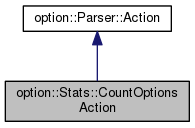
\includegraphics[width=218pt]{classoption_1_1Stats_1_1CountOptionsAction__inherit__graph}
\end{center}
\end{figure}


Collaboration diagram for option\+:\+:Stats\+:\+:Count\+Options\+Action\+:
\nopagebreak
\begin{figure}[H]
\begin{center}
\leavevmode
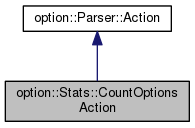
\includegraphics[width=218pt]{classoption_1_1Stats_1_1CountOptionsAction__coll__graph}
\end{center}
\end{figure}
\subsection*{Public Member Functions}
\begin{DoxyCompactItemize}
\item 
\hyperlink{classoption_1_1Stats_1_1CountOptionsAction_a24a38b87ad129b0e12660bd2019ba284}{Count\+Options\+Action} (unsigned $\ast$buffer\+\_\+max\+\_\+)
\item 
bool \hyperlink{classoption_1_1Stats_1_1CountOptionsAction_a29ab8a68d0a30736b99b4d2e5dece489}{perform} (\hyperlink{classoption_1_1Option}{Option} \&)
\begin{DoxyCompactList}\small\item\em Called by Parser\+::workhorse() for each \hyperlink{classoption_1_1Option}{Option} that has been successfully parsed (including unknown options if they have a \hyperlink{structoption_1_1Descriptor}{Descriptor} whose \hyperlink{structoption_1_1Descriptor_aa5d675dba0214a4abd73007ff163cc67}{Descriptor\+::check\+\_\+arg} does not return \hyperlink{namespaceoption_aee8c76a07877335762631491e7a5a1a9a9528e32563b795bd2930b12d0a5e382d}{A\+R\+G\+\_\+\+I\+L\+L\+E\+G\+AL}. \end{DoxyCompactList}\end{DoxyCompactItemize}


\subsection{Constructor \& Destructor Documentation}
\index{option\+::\+Stats\+::\+Count\+Options\+Action@{option\+::\+Stats\+::\+Count\+Options\+Action}!Count\+Options\+Action@{Count\+Options\+Action}}
\index{Count\+Options\+Action@{Count\+Options\+Action}!option\+::\+Stats\+::\+Count\+Options\+Action@{option\+::\+Stats\+::\+Count\+Options\+Action}}
\subsubsection[{\texorpdfstring{Count\+Options\+Action(unsigned $\ast$buffer\+\_\+max\+\_\+)}{CountOptionsAction(unsigned *buffer_max_)}}]{\setlength{\rightskip}{0pt plus 5cm}option\+::\+Stats\+::\+Count\+Options\+Action\+::\+Count\+Options\+Action (
\begin{DoxyParamCaption}
\item[{unsigned $\ast$}]{buffer\+\_\+max\+\_\+}
\end{DoxyParamCaption}
)\hspace{0.3cm}{\ttfamily [inline]}}\hypertarget{classoption_1_1Stats_1_1CountOptionsAction_a24a38b87ad129b0e12660bd2019ba284}{}\label{classoption_1_1Stats_1_1CountOptionsAction_a24a38b87ad129b0e12660bd2019ba284}
Creates a new \hyperlink{classoption_1_1Stats_1_1CountOptionsAction}{Count\+Options\+Action} that will increase {\ttfamily $\ast$buffer\+\_\+max\+\_\+} for each parsed \hyperlink{classoption_1_1Option}{Option}. 

\subsection{Member Function Documentation}
\index{option\+::\+Stats\+::\+Count\+Options\+Action@{option\+::\+Stats\+::\+Count\+Options\+Action}!perform@{perform}}
\index{perform@{perform}!option\+::\+Stats\+::\+Count\+Options\+Action@{option\+::\+Stats\+::\+Count\+Options\+Action}}
\subsubsection[{\texorpdfstring{perform(\+Option \&)}{perform(Option &)}}]{\setlength{\rightskip}{0pt plus 5cm}bool option\+::\+Stats\+::\+Count\+Options\+Action\+::perform (
\begin{DoxyParamCaption}
\item[{{\bf Option} \&}]{}
\end{DoxyParamCaption}
)\hspace{0.3cm}{\ttfamily [inline]}, {\ttfamily [virtual]}}\hypertarget{classoption_1_1Stats_1_1CountOptionsAction_a29ab8a68d0a30736b99b4d2e5dece489}{}\label{classoption_1_1Stats_1_1CountOptionsAction_a29ab8a68d0a30736b99b4d2e5dece489}


Called by Parser\+::workhorse() for each \hyperlink{classoption_1_1Option}{Option} that has been successfully parsed (including unknown options if they have a \hyperlink{structoption_1_1Descriptor}{Descriptor} whose \hyperlink{structoption_1_1Descriptor_aa5d675dba0214a4abd73007ff163cc67}{Descriptor\+::check\+\_\+arg} does not return \hyperlink{namespaceoption_aee8c76a07877335762631491e7a5a1a9a9528e32563b795bd2930b12d0a5e382d}{A\+R\+G\+\_\+\+I\+L\+L\+E\+G\+AL}. 

Returns {\ttfamily false} iff a fatal error has occured and the parse should be aborted. 

Reimplemented from \hyperlink{structoption_1_1Parser_1_1Action_a176b5f783bb35eb015b6d2c09422457d}{option\+::\+Parser\+::\+Action}.



The documentation for this class was generated from the following file\+:\begin{DoxyCompactItemize}
\item 
\hyperlink{optionparser_8h}{optionparser.\+h}\end{DoxyCompactItemize}

\hypertarget{structoption_1_1Descriptor}{}\section{option\+:\+:Descriptor Struct Reference}
\label{structoption_1_1Descriptor}\index{option\+::\+Descriptor@{option\+::\+Descriptor}}


Describes an option, its help text (usage) and how it should be parsed.  




{\ttfamily \#include $<$optionparser.\+h$>$}

\subsection*{Public Attributes}
\begin{DoxyCompactItemize}
\item 
const unsigned \hyperlink{structoption_1_1Descriptor_a1fee8ac44f529c99ac2b1149b4c391b1}{index}
\begin{DoxyCompactList}\small\item\em Index of this option\textquotesingle{}s linked list in the array filled in by the parser. \end{DoxyCompactList}\item 
const int \hyperlink{structoption_1_1Descriptor_a1b220dabd8aad075fa441a80f9b9343c}{type}
\begin{DoxyCompactList}\small\item\em Used to distinguish between options with the same \hyperlink{structoption_1_1Descriptor_a1fee8ac44f529c99ac2b1149b4c391b1}{index}. See \hyperlink{structoption_1_1Descriptor_a1fee8ac44f529c99ac2b1149b4c391b1}{index} for details. \end{DoxyCompactList}\item 
const char $\ast$const \hyperlink{structoption_1_1Descriptor_a0dba4ccca59c19d6ed4081391fca5adb}{shortopt}
\begin{DoxyCompactList}\small\item\em Each char in this string will be accepted as a short option character. \end{DoxyCompactList}\item 
const char $\ast$const \hyperlink{structoption_1_1Descriptor_a470c449dfa894c9bfda2dae026142b4b}{longopt}
\begin{DoxyCompactList}\small\item\em The long option name (without the leading {\ttfamily --} ). \end{DoxyCompactList}\item 
const \hyperlink{namespaceoption_a4cdf403efae65e18bf850e2001b12a2a}{Check\+Arg} \hyperlink{structoption_1_1Descriptor_aa5d675dba0214a4abd73007ff163cc67}{check\+\_\+arg}
\begin{DoxyCompactList}\small\item\em For each option that matches \hyperlink{structoption_1_1Descriptor_a0dba4ccca59c19d6ed4081391fca5adb}{shortopt} or \hyperlink{structoption_1_1Descriptor_a470c449dfa894c9bfda2dae026142b4b}{longopt} this function will be called to check a potential argument to the option. \end{DoxyCompactList}\item 
const char $\ast$ \hyperlink{structoption_1_1Descriptor_a9045b19311533e1b8a08645d57149c79}{help}
\begin{DoxyCompactList}\small\item\em The usage text associated with the options in this \hyperlink{structoption_1_1Descriptor}{Descriptor}. \end{DoxyCompactList}\end{DoxyCompactItemize}


\subsection{Detailed Description}
Describes an option, its help text (usage) and how it should be parsed. 

The main input when constructing an \hyperlink{classoption_1_1Parser}{option\+::\+Parser} is an array of Descriptors.

\begin{DoxyParagraph}{Example\+:}

\begin{DoxyCode}
\textcolor{keyword}{enum} OptionIndex \{CREATE, ...\};
\textcolor{keyword}{enum} OptionType \{DISABLE, ENABLE, OTHER\};

\textcolor{keyword}{const} \hyperlink{structoption_1_1Descriptor}{option::Descriptor} usage[] = \{
  \{ CREATE,                                            \textcolor{comment}{// index}
    OTHER,                                             \textcolor{comment}{// type}
    \textcolor{stringliteral}{"c"},                                               \textcolor{comment}{// shortopt}
    \textcolor{stringliteral}{"create"},                                          \textcolor{comment}{// longopt}
    \hyperlink{structoption_1_1Arg_a7fc01987899c91c6b6a1be5711a46e22}{Arg::None},                                         \textcolor{comment}{// check\_arg}
    \textcolor{stringliteral}{"--create  Tells the program to create something."} \textcolor{comment}{// help}
  \}
  , ...
\};
\end{DoxyCode}
 
\end{DoxyParagraph}


\subsection{Member Data Documentation}
\index{option\+::\+Descriptor@{option\+::\+Descriptor}!check\+\_\+arg@{check\+\_\+arg}}
\index{check\+\_\+arg@{check\+\_\+arg}!option\+::\+Descriptor@{option\+::\+Descriptor}}
\subsubsection[{\texorpdfstring{check\+\_\+arg}{check_arg}}]{\setlength{\rightskip}{0pt plus 5cm}const {\bf Check\+Arg} option\+::\+Descriptor\+::check\+\_\+arg}\hypertarget{structoption_1_1Descriptor_aa5d675dba0214a4abd73007ff163cc67}{}\label{structoption_1_1Descriptor_aa5d675dba0214a4abd73007ff163cc67}


For each option that matches \hyperlink{structoption_1_1Descriptor_a0dba4ccca59c19d6ed4081391fca5adb}{shortopt} or \hyperlink{structoption_1_1Descriptor_a470c449dfa894c9bfda2dae026142b4b}{longopt} this function will be called to check a potential argument to the option. 

This function will be called even if there is no potential argument. In that case it will be passed {\ttfamily N\+U\+LL} as {\ttfamily arg} parameter. Do not confuse this with the empty string.

See \hyperlink{namespaceoption_a4cdf403efae65e18bf850e2001b12a2a}{Check\+Arg} for more information. \index{option\+::\+Descriptor@{option\+::\+Descriptor}!help@{help}}
\index{help@{help}!option\+::\+Descriptor@{option\+::\+Descriptor}}
\subsubsection[{\texorpdfstring{help}{help}}]{\setlength{\rightskip}{0pt plus 5cm}const char$\ast$ option\+::\+Descriptor\+::help}\hypertarget{structoption_1_1Descriptor_a9045b19311533e1b8a08645d57149c79}{}\label{structoption_1_1Descriptor_a9045b19311533e1b8a08645d57149c79}


The usage text associated with the options in this \hyperlink{structoption_1_1Descriptor}{Descriptor}. 

You can use \hyperlink{namespaceoption_afc8bb7e040a98a0b33ff1ce9da1be0d1}{option\+::print\+Usage()} to format your usage message based on the {\ttfamily help} texts. You can use dummy Descriptors where \hyperlink{structoption_1_1Descriptor_a0dba4ccca59c19d6ed4081391fca5adb}{shortopt} and \hyperlink{structoption_1_1Descriptor_a470c449dfa894c9bfda2dae026142b4b}{longopt} are both the empty string to add text to the usage that is not related to a specific option.

See \hyperlink{namespaceoption_afc8bb7e040a98a0b33ff1ce9da1be0d1}{option\+::print\+Usage()} for special formatting characters you can use in {\ttfamily help} to get a column layout.

\begin{DoxyAttention}{Attention}
Must be U\+T\+F-\/8-\/encoded. If your compiler supports C++11 you can use the \char`\"{}u8\char`\"{} prefix to make sure string literals are properly encoded. 
\end{DoxyAttention}
\index{option\+::\+Descriptor@{option\+::\+Descriptor}!index@{index}}
\index{index@{index}!option\+::\+Descriptor@{option\+::\+Descriptor}}
\subsubsection[{\texorpdfstring{index}{index}}]{\setlength{\rightskip}{0pt plus 5cm}const unsigned option\+::\+Descriptor\+::index}\hypertarget{structoption_1_1Descriptor_a1fee8ac44f529c99ac2b1149b4c391b1}{}\label{structoption_1_1Descriptor_a1fee8ac44f529c99ac2b1149b4c391b1}


Index of this option\textquotesingle{}s linked list in the array filled in by the parser. 

Command line options whose Descriptors have the same index will end up in the same linked list in the order in which they appear on the command line. If you have multiple long option aliases that refer to the same option, give their descriptors the same {\ttfamily index}.

If you have options that mean exactly opposite things (e.\+g. {\ttfamily --enable-\/foo} and {\ttfamily --disable-\/foo} ), you should also give them the same {\ttfamily index}, but distinguish them through different values for \hyperlink{structoption_1_1Descriptor_a1b220dabd8aad075fa441a80f9b9343c}{type}. That way they end up in the same list and you can just take the last element of the list and use its type. This way you get the usual behaviour where switches later on the command line override earlier ones without having to code it manually.

\begin{DoxyParagraph}{Tip\+:}
Use an enum rather than plain ints for better readability, as shown in the example at \hyperlink{structoption_1_1Descriptor}{Descriptor}. 
\end{DoxyParagraph}
\index{option\+::\+Descriptor@{option\+::\+Descriptor}!longopt@{longopt}}
\index{longopt@{longopt}!option\+::\+Descriptor@{option\+::\+Descriptor}}
\subsubsection[{\texorpdfstring{longopt}{longopt}}]{\setlength{\rightskip}{0pt plus 5cm}const char$\ast$ const option\+::\+Descriptor\+::longopt}\hypertarget{structoption_1_1Descriptor_a470c449dfa894c9bfda2dae026142b4b}{}\label{structoption_1_1Descriptor_a470c449dfa894c9bfda2dae026142b4b}


The long option name (without the leading {\ttfamily --} ). 

If this \hyperlink{structoption_1_1Descriptor}{Descriptor} should not have a long option name, use the empty string \char`\"{}\char`\"{}. N\+U\+LL is not permitted here!

While \hyperlink{structoption_1_1Descriptor_a0dba4ccca59c19d6ed4081391fca5adb}{shortopt} allows multiple short option characters, each \hyperlink{structoption_1_1Descriptor}{Descriptor} can have only a single long option name. If you have multiple long option names referring to the same option use separate Descriptors that have the same \hyperlink{structoption_1_1Descriptor_a1fee8ac44f529c99ac2b1149b4c391b1}{index} and \hyperlink{structoption_1_1Descriptor_a1b220dabd8aad075fa441a80f9b9343c}{type}. You may repeat short option characters in such an alias \hyperlink{structoption_1_1Descriptor}{Descriptor} but there\textquotesingle{}s no need to.

\begin{DoxyParagraph}{Dummy Descriptors\+:}
You can use dummy Descriptors with an empty string for both \hyperlink{structoption_1_1Descriptor_a0dba4ccca59c19d6ed4081391fca5adb}{shortopt} and \hyperlink{structoption_1_1Descriptor_a470c449dfa894c9bfda2dae026142b4b}{longopt} to add text to the usage that is not related to a specific option. See \hyperlink{structoption_1_1Descriptor_a9045b19311533e1b8a08645d57149c79}{help}. The first dummy \hyperlink{structoption_1_1Descriptor}{Descriptor} will be used for unknown options (see below).
\end{DoxyParagraph}
\begin{DoxyParagraph}{Unknown Option Descriptor\+:}
The first dummy \hyperlink{structoption_1_1Descriptor}{Descriptor} in the list of Descriptors, whose \hyperlink{structoption_1_1Descriptor_a0dba4ccca59c19d6ed4081391fca5adb}{shortopt} and \hyperlink{structoption_1_1Descriptor_a470c449dfa894c9bfda2dae026142b4b}{longopt} are both the empty string, will be used as the \hyperlink{structoption_1_1Descriptor}{Descriptor} for unknown options. An unknown option is a string in the argument vector that is not a lone minus {\ttfamily \textquotesingle{}-\/\textquotesingle{}} but starts with a minus character and does not match any \hyperlink{structoption_1_1Descriptor}{Descriptor}\textquotesingle{}s \hyperlink{structoption_1_1Descriptor_a0dba4ccca59c19d6ed4081391fca5adb}{shortopt} or \hyperlink{structoption_1_1Descriptor_a470c449dfa894c9bfda2dae026142b4b}{longopt}. ~\newline
Note that the dummy descriptor\textquotesingle{}s \hyperlink{structoption_1_1Descriptor_aa5d675dba0214a4abd73007ff163cc67}{check\+\_\+arg} function {\itshape will} be called and its return value will be evaluated as usual. I.\+e. if it returns \hyperlink{namespaceoption_aee8c76a07877335762631491e7a5a1a9a9528e32563b795bd2930b12d0a5e382d}{A\+R\+G\+\_\+\+I\+L\+L\+E\+G\+AL} the parsing will be aborted with {\ttfamily \hyperlink{classoption_1_1Parser_a2caa149140067b4d13e4d7a104bb3090}{Parser\+::error()}==true}. ~\newline
if {\ttfamily check\+\_\+arg} does not return \hyperlink{namespaceoption_aee8c76a07877335762631491e7a5a1a9a9528e32563b795bd2930b12d0a5e382d}{A\+R\+G\+\_\+\+I\+L\+L\+E\+G\+AL} the descriptor\textquotesingle{}s \hyperlink{structoption_1_1Descriptor_a1fee8ac44f529c99ac2b1149b4c391b1}{index} {\itshape will} be used to pick the linked list into which to put the unknown option. ~\newline
If there is no dummy descriptor, unknown options will be dropped silently. 
\end{DoxyParagraph}
\index{option\+::\+Descriptor@{option\+::\+Descriptor}!shortopt@{shortopt}}
\index{shortopt@{shortopt}!option\+::\+Descriptor@{option\+::\+Descriptor}}
\subsubsection[{\texorpdfstring{shortopt}{shortopt}}]{\setlength{\rightskip}{0pt plus 5cm}const char$\ast$ const option\+::\+Descriptor\+::shortopt}\hypertarget{structoption_1_1Descriptor_a0dba4ccca59c19d6ed4081391fca5adb}{}\label{structoption_1_1Descriptor_a0dba4ccca59c19d6ed4081391fca5adb}


Each char in this string will be accepted as a short option character. 

The string must not include the minus character {\ttfamily \textquotesingle{}-\/\textquotesingle{}} or you\textquotesingle{}ll get undefined behaviour.

If this \hyperlink{structoption_1_1Descriptor}{Descriptor} should not have short option characters, use the empty string \char`\"{}\char`\"{}. N\+U\+LL is not permitted here!

See \hyperlink{structoption_1_1Descriptor_a470c449dfa894c9bfda2dae026142b4b}{longopt} for more information. \index{option\+::\+Descriptor@{option\+::\+Descriptor}!type@{type}}
\index{type@{type}!option\+::\+Descriptor@{option\+::\+Descriptor}}
\subsubsection[{\texorpdfstring{type}{type}}]{\setlength{\rightskip}{0pt plus 5cm}const int option\+::\+Descriptor\+::type}\hypertarget{structoption_1_1Descriptor_a1b220dabd8aad075fa441a80f9b9343c}{}\label{structoption_1_1Descriptor_a1b220dabd8aad075fa441a80f9b9343c}


Used to distinguish between options with the same \hyperlink{structoption_1_1Descriptor_a1fee8ac44f529c99ac2b1149b4c391b1}{index}. See \hyperlink{structoption_1_1Descriptor_a1fee8ac44f529c99ac2b1149b4c391b1}{index} for details. 

It is recommended that you use an enum rather than a plain int to make your code more readable. 

The documentation for this struct was generated from the following file\+:\begin{DoxyCompactItemize}
\item 
\hyperlink{optionparser_8h}{optionparser.\+h}\end{DoxyCompactItemize}

\hypertarget{classhebi_1_1Info_1_1EnumField}{}\section{hebi\+:\+:Info\+:\+:Enum\+Field$<$ T $>$ Class Template Reference}
\label{classhebi_1_1Info_1_1EnumField}\index{hebi\+::\+Info\+::\+Enum\+Field$<$ T $>$@{hebi\+::\+Info\+::\+Enum\+Field$<$ T $>$}}


A message field representable by an enum of a given type.  




{\ttfamily \#include $<$info.\+hpp$>$}

\subsection*{Public Member Functions}
\begin{DoxyCompactItemize}
\item 
\mbox{\Hypertarget{classhebi_1_1Info_1_1EnumField_ad4680cb2ff477ed2dfb4ae47f0fd6836}\label{classhebi_1_1Info_1_1EnumField_ad4680cb2ff477ed2dfb4ae47f0fd6836}} 
{\bfseries Enum\+Field} (Hebi\+Info\+Ptr internal, Info\+Enum\+Field field)
\item 
\hyperlink{classhebi_1_1Info_1_1EnumField_ac1690565ae2d937a18f9c39e3b1111ed}{operator bool} () const
\begin{DoxyCompactList}\small\item\em Allows casting to a bool to check if the field has a value without directly calling {\ttfamily \hyperlink{classhebi_1_1Info_1_1EnumField_a1c8fe912ecc7e5d7f8f3d8f0fa346ba9}{has()}}. \end{DoxyCompactList}\item 
\mbox{\Hypertarget{classhebi_1_1Info_1_1EnumField_a1c8fe912ecc7e5d7f8f3d8f0fa346ba9}\label{classhebi_1_1Info_1_1EnumField_a1c8fe912ecc7e5d7f8f3d8f0fa346ba9}} 
bool \hyperlink{classhebi_1_1Info_1_1EnumField_a1c8fe912ecc7e5d7f8f3d8f0fa346ba9}{has} () const
\begin{DoxyCompactList}\small\item\em True if (and only if) the field has a value. \end{DoxyCompactList}\item 
\mbox{\Hypertarget{classhebi_1_1Info_1_1EnumField_adbb07d48e17f3ec031bfc5a24c810cf2}\label{classhebi_1_1Info_1_1EnumField_adbb07d48e17f3ec031bfc5a24c810cf2}} 
T \hyperlink{classhebi_1_1Info_1_1EnumField_adbb07d48e17f3ec031bfc5a24c810cf2}{get} () const
\begin{DoxyCompactList}\small\item\em If the field has a value, returns that value; otherwise, returns a default. \end{DoxyCompactList}\end{DoxyCompactItemize}


\subsection{Detailed Description}
\subsubsection*{template$<$class T$>$\newline
class hebi\+::\+Info\+::\+Enum\+Field$<$ T $>$}

A message field representable by an enum of a given type. 

\subsection{Member Function Documentation}
\mbox{\Hypertarget{classhebi_1_1Info_1_1EnumField_ac1690565ae2d937a18f9c39e3b1111ed}\label{classhebi_1_1Info_1_1EnumField_ac1690565ae2d937a18f9c39e3b1111ed}} 
\index{hebi\+::\+Info\+::\+Enum\+Field@{hebi\+::\+Info\+::\+Enum\+Field}!operator bool@{operator bool}}
\index{operator bool@{operator bool}!hebi\+::\+Info\+::\+Enum\+Field@{hebi\+::\+Info\+::\+Enum\+Field}}
\subsubsection{\texorpdfstring{operator bool()}{operator bool()}}
{\footnotesize\ttfamily template$<$class T$>$ \\
\hyperlink{classhebi_1_1Info_1_1EnumField}{hebi\+::\+Info\+::\+Enum\+Field}$<$ T $>$\+::operator bool (\begin{DoxyParamCaption}{ }\end{DoxyParamCaption}) const\hspace{0.3cm}{\ttfamily [inline]}, {\ttfamily [explicit]}}



Allows casting to a bool to check if the field has a value without directly calling {\ttfamily \hyperlink{classhebi_1_1Info_1_1EnumField_a1c8fe912ecc7e5d7f8f3d8f0fa346ba9}{has()}}. 

This can be used as in the following (assuming \textquotesingle{}parent\textquotesingle{} is a parent message, and this field is called \textquotesingle{}my\+Field\textquotesingle{}) 
\begin{DoxyCode}
Info::EnumField& f = parent.myField();
\textcolor{keywordflow}{if} (f)
  std::cout << \textcolor{stringliteral}{"Field has value: "} << f.get() << std::endl;
\textcolor{keywordflow}{else}
  std::cout << \textcolor{stringliteral}{"Field has no value!"} << std::endl;
\end{DoxyCode}
 

The documentation for this class was generated from the following file\+:\begin{DoxyCompactItemize}
\item 
info.\+hpp\end{DoxyCompactItemize}

\hypertarget{classhebi_1_1Command_1_1EnumField}{}\section{hebi\+:\+:Command\+:\+:Enum\+Field$<$ T $>$ Class Template Reference}
\label{classhebi_1_1Command_1_1EnumField}\index{hebi\+::\+Command\+::\+Enum\+Field$<$ T $>$@{hebi\+::\+Command\+::\+Enum\+Field$<$ T $>$}}


A message field representable by an enum of a given type.  




{\ttfamily \#include $<$command.\+hpp$>$}

\subsection*{Public Member Functions}
\begin{DoxyCompactItemize}
\item 
{\bfseries Enum\+Field} (Hebi\+Command\+Ptr internal, Command\+Enum\+Field field)\hypertarget{classhebi_1_1Command_1_1EnumField_aa2a658eb3d71afcdeb2a47a65414bb89}{}\label{classhebi_1_1Command_1_1EnumField_aa2a658eb3d71afcdeb2a47a65414bb89}

\item 
\hyperlink{classhebi_1_1Command_1_1EnumField_aef3f83474be1d547c835e7c7ea8169ef}{operator bool} () const 
\begin{DoxyCompactList}\small\item\em Allows casting to a bool to check if the field has a value without directly calling {\ttfamily \hyperlink{classhebi_1_1Command_1_1EnumField_a9dde151d6155a016ba0d79b7dca0488a}{has()}}. \end{DoxyCompactList}\item 
bool \hyperlink{classhebi_1_1Command_1_1EnumField_a9dde151d6155a016ba0d79b7dca0488a}{has} () const \hypertarget{classhebi_1_1Command_1_1EnumField_a9dde151d6155a016ba0d79b7dca0488a}{}\label{classhebi_1_1Command_1_1EnumField_a9dde151d6155a016ba0d79b7dca0488a}

\begin{DoxyCompactList}\small\item\em True if (and only if) the field has a value. \end{DoxyCompactList}\item 
T \hyperlink{classhebi_1_1Command_1_1EnumField_a1ee97c72049de10f4cd0541d395d6286}{get} () const \hypertarget{classhebi_1_1Command_1_1EnumField_a1ee97c72049de10f4cd0541d395d6286}{}\label{classhebi_1_1Command_1_1EnumField_a1ee97c72049de10f4cd0541d395d6286}

\begin{DoxyCompactList}\small\item\em If the field has a value, returns that value; otherwise, returns a default. \end{DoxyCompactList}\item 
void \hyperlink{classhebi_1_1Command_1_1EnumField_abdd656f051b4fc58cfc206ceb07a5b17}{set} (T value)\hypertarget{classhebi_1_1Command_1_1EnumField_abdd656f051b4fc58cfc206ceb07a5b17}{}\label{classhebi_1_1Command_1_1EnumField_abdd656f051b4fc58cfc206ceb07a5b17}

\begin{DoxyCompactList}\small\item\em Sets the field to a given value. \end{DoxyCompactList}\item 
void \hyperlink{classhebi_1_1Command_1_1EnumField_aa05f2160dbc34d73877ee308f71130a1}{clear} ()\hypertarget{classhebi_1_1Command_1_1EnumField_aa05f2160dbc34d73877ee308f71130a1}{}\label{classhebi_1_1Command_1_1EnumField_aa05f2160dbc34d73877ee308f71130a1}

\begin{DoxyCompactList}\small\item\em Removes any currently set value for this field. \end{DoxyCompactList}\end{DoxyCompactItemize}


\subsection{Detailed Description}
\subsubsection*{template$<$class T$>$\\*
class hebi\+::\+Command\+::\+Enum\+Field$<$ T $>$}

A message field representable by an enum of a given type. 

\subsection{Member Function Documentation}
\index{hebi\+::\+Command\+::\+Enum\+Field@{hebi\+::\+Command\+::\+Enum\+Field}!operator bool@{operator bool}}
\index{operator bool@{operator bool}!hebi\+::\+Command\+::\+Enum\+Field@{hebi\+::\+Command\+::\+Enum\+Field}}
\subsubsection[{\texorpdfstring{operator bool() const }{operator bool() const }}]{\setlength{\rightskip}{0pt plus 5cm}template$<$class T$>$ {\bf hebi\+::\+Command\+::\+Enum\+Field}$<$ T $>$\+::operator bool (
\begin{DoxyParamCaption}
{}
\end{DoxyParamCaption}
) const\hspace{0.3cm}{\ttfamily [inline]}, {\ttfamily [explicit]}}\hypertarget{classhebi_1_1Command_1_1EnumField_aef3f83474be1d547c835e7c7ea8169ef}{}\label{classhebi_1_1Command_1_1EnumField_aef3f83474be1d547c835e7c7ea8169ef}


Allows casting to a bool to check if the field has a value without directly calling {\ttfamily \hyperlink{classhebi_1_1Command_1_1EnumField_a9dde151d6155a016ba0d79b7dca0488a}{has()}}. 

This can be used as in the following (assuming \textquotesingle{}parent\textquotesingle{} is a parent message, and this field is called \textquotesingle{}my\+Field\textquotesingle{}) 
\begin{DoxyCode}
Command::EnumField& f = parent.myField();
\textcolor{keywordflow}{if} (f)
  std::cout << \textcolor{stringliteral}{"Field has value: "} << f.get() << std::endl;
\textcolor{keywordflow}{else}
  std::cout << \textcolor{stringliteral}{"Field has no value!"} << std::endl;
\end{DoxyCode}
 

The documentation for this class was generated from the following file\+:\begin{DoxyCompactItemize}
\item 
command.\+hpp\end{DoxyCompactItemize}

\hypertarget{classhebi_1_1Feedback}{}\section{hebi\+:\+:Feedback Class Reference}
\label{classhebi_1_1Feedback}\index{hebi\+::\+Feedback@{hebi\+::\+Feedback}}


\hyperlink{classhebi_1_1Feedback}{Feedback} objects have various fields representing feedback from modules; which fields are populated depends on the module type and various other settings.  




{\ttfamily \#include $<$feedback.\+hpp$>$}

\subsection*{Classes}
\begin{DoxyCompactItemize}
\item 
class \hyperlink{classhebi_1_1Feedback_1_1Actuator}{Actuator}
\begin{DoxyCompactList}\small\item\em Actuator-\/specific feedback. \end{DoxyCompactList}\item 
class \hyperlink{classhebi_1_1Feedback_1_1FloatField}{Float\+Field}
\begin{DoxyCompactList}\small\item\em A message field representable by a single-\/precision floating point value. \end{DoxyCompactList}\item 
class \hyperlink{classhebi_1_1Feedback_1_1HighResAngleField}{High\+Res\+Angle\+Field}
\begin{DoxyCompactList}\small\item\em A message field for an angle measurement which does not lose precision at very high angles. \end{DoxyCompactList}\item 
class \hyperlink{classhebi_1_1Feedback_1_1Imu}{Imu}
\begin{DoxyCompactList}\small\item\em Inertial measurement unit feedback (accelerometers and gyros). \end{DoxyCompactList}\item 
class \hyperlink{classhebi_1_1Feedback_1_1LedField}{Led\+Field}
\begin{DoxyCompactList}\small\item\em A message field for interfacing with an L\+ED. \end{DoxyCompactList}\item 
class \hyperlink{classhebi_1_1Feedback_1_1NumberedFloatField}{Numbered\+Float\+Field}
\begin{DoxyCompactList}\small\item\em A message field containing a numbered set of single-\/precision floating point values. \end{DoxyCompactList}\item 
class \hyperlink{classhebi_1_1Feedback_1_1Vector3fField}{Vector3f\+Field}
\begin{DoxyCompactList}\small\item\em A message field representable by a 3-\/D vector of single-\/precision floating point values. \end{DoxyCompactList}\end{DoxyCompactItemize}
\subsection*{Public Member Functions}
\begin{DoxyCompactItemize}
\item 
\hyperlink{classhebi_1_1Feedback_aa24d88a1a9f74231e74d75a09ca3f2d8}{Feedback} ()\hypertarget{classhebi_1_1Feedback_aa24d88a1a9f74231e74d75a09ca3f2d8}{}\label{classhebi_1_1Feedback_aa24d88a1a9f74231e74d75a09ca3f2d8}

\begin{DoxyCompactList}\small\item\em Create a new feedback object for a single module. \end{DoxyCompactList}\item 
\hyperlink{classhebi_1_1Feedback_a172321e2516f2bca57a1e32d0263bd3f}{Feedback} (Hebi\+Feedback\+Ptr feedback)
\begin{DoxyCompactList}\small\item\em Wraps an existing C-\/style feedback object; object lifetime is assumed to be managed by the caller. \end{DoxyCompactList}\item 
\hyperlink{classhebi_1_1Feedback_ab2d48835e8c66094b5f058d52d95417f}{Feedback} (\hyperlink{classhebi_1_1Feedback}{Feedback} \&\&other)\hypertarget{classhebi_1_1Feedback_ab2d48835e8c66094b5f058d52d95417f}{}\label{classhebi_1_1Feedback_ab2d48835e8c66094b5f058d52d95417f}

\begin{DoxyCompactList}\small\item\em Move constructor (necessary for containment in S\+TL template classes) \end{DoxyCompactList}\item 
virtual \hyperlink{classhebi_1_1Feedback_a4d4b06211530ace089ec434f0c742b68}{$\sim$\+Feedback} () noexcept\hypertarget{classhebi_1_1Feedback_a4d4b06211530ace089ec434f0c742b68}{}\label{classhebi_1_1Feedback_a4d4b06211530ace089ec434f0c742b68}

\begin{DoxyCompactList}\small\item\em Destructor cleans up feedback object as necessary. \end{DoxyCompactList}\item 
const \hyperlink{classhebi_1_1Feedback_1_1Actuator}{Actuator} \& \hyperlink{classhebi_1_1Feedback_aba9c2b0fa8c94aeda647dd4ad99db0b1}{actuator} () const \hypertarget{classhebi_1_1Feedback_aba9c2b0fa8c94aeda647dd4ad99db0b1}{}\label{classhebi_1_1Feedback_aba9c2b0fa8c94aeda647dd4ad99db0b1}

\begin{DoxyCompactList}\small\item\em Actuator-\/specific feedback. \end{DoxyCompactList}\item 
const \hyperlink{classhebi_1_1Feedback_1_1Imu}{Imu} \& \hyperlink{classhebi_1_1Feedback_a9907e5aaab3eeaadfee842b0288768d8}{imu} () const \hypertarget{classhebi_1_1Feedback_a9907e5aaab3eeaadfee842b0288768d8}{}\label{classhebi_1_1Feedback_a9907e5aaab3eeaadfee842b0288768d8}

\begin{DoxyCompactList}\small\item\em Inertial measurement unit feedback (accelerometers and gyros). \end{DoxyCompactList}\item 
const \hyperlink{classhebi_1_1Feedback_1_1FloatField}{Float\+Field} \& \hyperlink{classhebi_1_1Feedback_a9e95dacddaa6ca0fa4f3fb0a7a31d9b2}{board\+Temperature} () const \hypertarget{classhebi_1_1Feedback_a9e95dacddaa6ca0fa4f3fb0a7a31d9b2}{}\label{classhebi_1_1Feedback_a9e95dacddaa6ca0fa4f3fb0a7a31d9b2}

\begin{DoxyCompactList}\small\item\em Ambient temperature inside the module (measured at the I\+MU chip), in degrees Celsius. \end{DoxyCompactList}\item 
const \hyperlink{classhebi_1_1Feedback_1_1FloatField}{Float\+Field} \& \hyperlink{classhebi_1_1Feedback_a13cc72584b6d65cad80c90b4ecbb6a72}{processor\+Temperature} () const \hypertarget{classhebi_1_1Feedback_a13cc72584b6d65cad80c90b4ecbb6a72}{}\label{classhebi_1_1Feedback_a13cc72584b6d65cad80c90b4ecbb6a72}

\begin{DoxyCompactList}\small\item\em Temperature of the processor chip, in degrees Celsius. \end{DoxyCompactList}\item 
const \hyperlink{classhebi_1_1Feedback_1_1FloatField}{Float\+Field} \& \hyperlink{classhebi_1_1Feedback_a9aac48c0a099fc2a540280f0e3e30eca}{voltage} () const \hypertarget{classhebi_1_1Feedback_a9aac48c0a099fc2a540280f0e3e30eca}{}\label{classhebi_1_1Feedback_a9aac48c0a099fc2a540280f0e3e30eca}

\begin{DoxyCompactList}\small\item\em Bus voltage that the module is running at (in Volts). \end{DoxyCompactList}\item 
const \hyperlink{classhebi_1_1Feedback_1_1NumberedFloatField}{Numbered\+Float\+Field} \& \hyperlink{classhebi_1_1Feedback_aaeb6f51987d003d4f9168975b8292d9d}{debug} () const \hypertarget{classhebi_1_1Feedback_aaeb6f51987d003d4f9168975b8292d9d}{}\label{classhebi_1_1Feedback_aaeb6f51987d003d4f9168975b8292d9d}

\begin{DoxyCompactList}\small\item\em Values for internal debug functions (channel 1-\/9 available). \end{DoxyCompactList}\item 
const \hyperlink{classhebi_1_1Feedback_1_1LedField}{Led\+Field} \& \hyperlink{classhebi_1_1Feedback_a96a52d85fc278e41e3957ff9c741241b}{led} () const \hypertarget{classhebi_1_1Feedback_a96a52d85fc278e41e3957ff9c741241b}{}\label{classhebi_1_1Feedback_a96a52d85fc278e41e3957ff9c741241b}

\begin{DoxyCompactList}\small\item\em The module\textquotesingle{}s L\+ED. \end{DoxyCompactList}\end{DoxyCompactItemize}
\subsection*{Public Attributes}
\begin{DoxyCompactItemize}
\item 
Hebi\+Feedback\+Ptr const \hyperlink{classhebi_1_1Feedback_ae91da5bbb8a77c135981df418d7515b1}{internal\+\_\+}
\end{DoxyCompactItemize}


\subsection{Detailed Description}
\hyperlink{classhebi_1_1Feedback}{Feedback} objects have various fields representing feedback from modules; which fields are populated depends on the module type and various other settings. 

This object has a hierarchical structure -- there are some direct general-\/purpose fields at the top level, and many more specific fields contained in different nested subobjects.

The subobjects contain references to the parent feedback object, and so should not be used after the parent object has been destroyed.

The fields in the feedback object are typed; generally, these are optional-\/style read-\/only fields (i.\+e., have the concept of has/get), although the return types and exact interface vary slightly between fields. Where appropriate, the explicit bool operator has been overridden so that you can shortcut {\ttfamily if}(field.\+has()) by calling {\ttfamily if(field)}.

Although this header file can be used to look at the hierarchy of the messages, in general the online documentation at apidocs.\+hebi.\+us presents this information. in a more readable form. 

\subsection{Constructor \& Destructor Documentation}
\index{hebi\+::\+Feedback@{hebi\+::\+Feedback}!Feedback@{Feedback}}
\index{Feedback@{Feedback}!hebi\+::\+Feedback@{hebi\+::\+Feedback}}
\subsubsection[{\texorpdfstring{Feedback(\+Hebi\+Feedback\+Ptr feedback)}{Feedback(HebiFeedbackPtr feedback)}}]{\setlength{\rightskip}{0pt plus 5cm}hebi\+::\+Feedback\+::\+Feedback (
\begin{DoxyParamCaption}
\item[{Hebi\+Feedback\+Ptr}]{feedback}
\end{DoxyParamCaption}
)}\hypertarget{classhebi_1_1Feedback_a172321e2516f2bca57a1e32d0263bd3f}{}\label{classhebi_1_1Feedback_a172321e2516f2bca57a1e32d0263bd3f}


Wraps an existing C-\/style feedback object; object lifetime is assumed to be managed by the caller. 

N\+O\+TE\+: this should not be used except by internal library functions! 

\subsection{Member Data Documentation}
\index{hebi\+::\+Feedback@{hebi\+::\+Feedback}!internal\+\_\+@{internal\+\_\+}}
\index{internal\+\_\+@{internal\+\_\+}!hebi\+::\+Feedback@{hebi\+::\+Feedback}}
\subsubsection[{\texorpdfstring{internal\+\_\+}{internal_}}]{\setlength{\rightskip}{0pt plus 5cm}Hebi\+Feedback\+Ptr const hebi\+::\+Feedback\+::internal\+\_\+}\hypertarget{classhebi_1_1Feedback_ae91da5bbb8a77c135981df418d7515b1}{}\label{classhebi_1_1Feedback_ae91da5bbb8a77c135981df418d7515b1}
C-\/style feedback object. N\+O\+TE\+: this should not be used except by internal library functions! 

The documentation for this class was generated from the following files\+:\begin{DoxyCompactItemize}
\item 
feedback.\+hpp\item 
feedback.\+cpp\end{DoxyCompactItemize}

\hypertarget{classhebi_1_1Info_1_1FlagField}{}\section{hebi\+:\+:Info\+:\+:Flag\+Field Class Reference}
\label{classhebi_1_1Info_1_1FlagField}\index{hebi\+::\+Info\+::\+Flag\+Field@{hebi\+::\+Info\+::\+Flag\+Field}}


A two-\/state message field (either set/true or cleared/false).  




{\ttfamily \#include $<$info.\+hpp$>$}

\subsection*{Public Member Functions}
\begin{DoxyCompactItemize}
\item 
{\bfseries Flag\+Field} (Hebi\+Info\+Ptr internal, Info\+Flag\+Field field)\hypertarget{classhebi_1_1Info_1_1FlagField_a2c779f542b33a5ac7dbd020b6a56bccf}{}\label{classhebi_1_1Info_1_1FlagField_a2c779f542b33a5ac7dbd020b6a56bccf}

\item 
\hyperlink{classhebi_1_1Info_1_1FlagField_a14b2e23f77976afe5defcef5c00eb7aa}{operator bool} () const 
\begin{DoxyCompactList}\small\item\em Allows casting to a bool to check if the flag is set without directly calling {\ttfamily \hyperlink{classhebi_1_1Info_1_1FlagField_a497aad19d402401c286eba2db9d86d5e}{has()}}. \end{DoxyCompactList}\item 
bool \hyperlink{classhebi_1_1Info_1_1FlagField_a497aad19d402401c286eba2db9d86d5e}{has} () const \hypertarget{classhebi_1_1Info_1_1FlagField_a497aad19d402401c286eba2db9d86d5e}{}\label{classhebi_1_1Info_1_1FlagField_a497aad19d402401c286eba2db9d86d5e}

\begin{DoxyCompactList}\small\item\em Returns {\ttfamily true} if the flag is set, false if it is cleared. \end{DoxyCompactList}\end{DoxyCompactItemize}


\subsection{Detailed Description}
A two-\/state message field (either set/true or cleared/false). 

\subsection{Member Function Documentation}
\index{hebi\+::\+Info\+::\+Flag\+Field@{hebi\+::\+Info\+::\+Flag\+Field}!operator bool@{operator bool}}
\index{operator bool@{operator bool}!hebi\+::\+Info\+::\+Flag\+Field@{hebi\+::\+Info\+::\+Flag\+Field}}
\subsubsection[{\texorpdfstring{operator bool() const }{operator bool() const }}]{\setlength{\rightskip}{0pt plus 5cm}hebi\+::\+Info\+::\+Flag\+Field\+::operator bool (
\begin{DoxyParamCaption}
{}
\end{DoxyParamCaption}
) const\hspace{0.3cm}{\ttfamily [explicit]}}\hypertarget{classhebi_1_1Info_1_1FlagField_a14b2e23f77976afe5defcef5c00eb7aa}{}\label{classhebi_1_1Info_1_1FlagField_a14b2e23f77976afe5defcef5c00eb7aa}


Allows casting to a bool to check if the flag is set without directly calling {\ttfamily \hyperlink{classhebi_1_1Info_1_1FlagField_a497aad19d402401c286eba2db9d86d5e}{has()}}. 

This can be used as in the following (assuming \textquotesingle{}parent\textquotesingle{} is a parent message, and this field is called \textquotesingle{}my\+Field\textquotesingle{}) 
\begin{DoxyCode}
Info::FlagField& f = parent.myField();
\textcolor{keywordflow}{if} (f)
  std::cout << \textcolor{stringliteral}{"Field has value: "} << f.get() << std::endl;
\textcolor{keywordflow}{else}
  std::cout << \textcolor{stringliteral}{"Field has no value!"} << std::endl;
\end{DoxyCode}
 

The documentation for this class was generated from the following files\+:\begin{DoxyCompactItemize}
\item 
info.\+hpp\item 
info.\+cpp\end{DoxyCompactItemize}

\hypertarget{classhebi_1_1Command_1_1FlagField}{}\section{hebi\+:\+:Command\+:\+:Flag\+Field Class Reference}
\label{classhebi_1_1Command_1_1FlagField}\index{hebi\+::\+Command\+::\+Flag\+Field@{hebi\+::\+Command\+::\+Flag\+Field}}


A two-\/state message field (either set/true or cleared/false).  




{\ttfamily \#include $<$command.\+hpp$>$}

\subsection*{Public Member Functions}
\begin{DoxyCompactItemize}
\item 
\mbox{\Hypertarget{classhebi_1_1Command_1_1FlagField_a4252702a9af7fe9b656d360d8ff7f14e}\label{classhebi_1_1Command_1_1FlagField_a4252702a9af7fe9b656d360d8ff7f14e}} 
{\bfseries Flag\+Field} (Hebi\+Command\+Ptr internal, Command\+Flag\+Field field)
\item 
\hyperlink{classhebi_1_1Command_1_1FlagField_afbe105fefc252d9a0036bc540729287b}{operator bool} () const
\begin{DoxyCompactList}\small\item\em Allows casting to a bool to check if the flag is set without directly calling {\ttfamily \hyperlink{classhebi_1_1Command_1_1FlagField_aa1493ce350be33e099dde81586e9ac3c}{has()}}. \end{DoxyCompactList}\item 
\mbox{\Hypertarget{classhebi_1_1Command_1_1FlagField_aa1493ce350be33e099dde81586e9ac3c}\label{classhebi_1_1Command_1_1FlagField_aa1493ce350be33e099dde81586e9ac3c}} 
bool \hyperlink{classhebi_1_1Command_1_1FlagField_aa1493ce350be33e099dde81586e9ac3c}{has} () const
\begin{DoxyCompactList}\small\item\em Returns {\ttfamily true} if the flag is set, false if it is cleared. \end{DoxyCompactList}\item 
\mbox{\Hypertarget{classhebi_1_1Command_1_1FlagField_a51fa751950973f51359f628b2714b683}\label{classhebi_1_1Command_1_1FlagField_a51fa751950973f51359f628b2714b683}} 
void \hyperlink{classhebi_1_1Command_1_1FlagField_a51fa751950973f51359f628b2714b683}{set} ()
\begin{DoxyCompactList}\small\item\em Sets this flag. \end{DoxyCompactList}\item 
\mbox{\Hypertarget{classhebi_1_1Command_1_1FlagField_aaf1399b14ddc9052ebbca70df5b638d3}\label{classhebi_1_1Command_1_1FlagField_aaf1399b14ddc9052ebbca70df5b638d3}} 
void \hyperlink{classhebi_1_1Command_1_1FlagField_aaf1399b14ddc9052ebbca70df5b638d3}{clear} ()
\begin{DoxyCompactList}\small\item\em Clears this flag (e.\+g., sets it to false/off). \end{DoxyCompactList}\end{DoxyCompactItemize}


\subsection{Detailed Description}
A two-\/state message field (either set/true or cleared/false). 

\subsection{Member Function Documentation}
\mbox{\Hypertarget{classhebi_1_1Command_1_1FlagField_afbe105fefc252d9a0036bc540729287b}\label{classhebi_1_1Command_1_1FlagField_afbe105fefc252d9a0036bc540729287b}} 
\index{hebi\+::\+Command\+::\+Flag\+Field@{hebi\+::\+Command\+::\+Flag\+Field}!operator bool@{operator bool}}
\index{operator bool@{operator bool}!hebi\+::\+Command\+::\+Flag\+Field@{hebi\+::\+Command\+::\+Flag\+Field}}
\subsubsection{\texorpdfstring{operator bool()}{operator bool()}}
{\footnotesize\ttfamily hebi\+::\+Command\+::\+Flag\+Field\+::operator bool (\begin{DoxyParamCaption}{ }\end{DoxyParamCaption}) const\hspace{0.3cm}{\ttfamily [explicit]}}



Allows casting to a bool to check if the flag is set without directly calling {\ttfamily \hyperlink{classhebi_1_1Command_1_1FlagField_aa1493ce350be33e099dde81586e9ac3c}{has()}}. 

This can be used as in the following (assuming \textquotesingle{}parent\textquotesingle{} is a parent message, and this field is called \textquotesingle{}my\+Field\textquotesingle{}) 
\begin{DoxyCode}
Command::FlagField& f = parent.myField();
\textcolor{keywordflow}{if} (f)
  std::cout << \textcolor{stringliteral}{"Field has value: "} << f.get() << std::endl;
\textcolor{keywordflow}{else}
  std::cout << \textcolor{stringliteral}{"Field has no value!"} << std::endl;
\end{DoxyCode}
 

The documentation for this class was generated from the following files\+:\begin{DoxyCompactItemize}
\item 
command.\+hpp\item 
command.\+cpp\end{DoxyCompactItemize}

\hypertarget{classhebi_1_1Command_1_1FloatField}{}\section{hebi\+:\+:Command\+:\+:Float\+Field Class Reference}
\label{classhebi_1_1Command_1_1FloatField}\index{hebi\+::\+Command\+::\+Float\+Field@{hebi\+::\+Command\+::\+Float\+Field}}


A message field representable by a single-\/precision floating point value.  




{\ttfamily \#include $<$command.\+hpp$>$}

\subsection*{Public Member Functions}
\begin{DoxyCompactItemize}
\item 
{\bfseries Float\+Field} (Hebi\+Command\+Ptr internal, Command\+Float\+Field field)\hypertarget{classhebi_1_1Command_1_1FloatField_a4eb2e80bc5c55e9dc87bba49430278c5}{}\label{classhebi_1_1Command_1_1FloatField_a4eb2e80bc5c55e9dc87bba49430278c5}

\item 
\hyperlink{classhebi_1_1Command_1_1FloatField_ae4983503c21f98ec479cc1bb73390754}{operator bool} () const 
\begin{DoxyCompactList}\small\item\em Allows casting to a bool to check if the field has a value without directly calling {\ttfamily \hyperlink{classhebi_1_1Command_1_1FloatField_a7220a798fceba4d3256d677b169359f1}{has()}}. \end{DoxyCompactList}\item 
bool \hyperlink{classhebi_1_1Command_1_1FloatField_a7220a798fceba4d3256d677b169359f1}{has} () const \hypertarget{classhebi_1_1Command_1_1FloatField_a7220a798fceba4d3256d677b169359f1}{}\label{classhebi_1_1Command_1_1FloatField_a7220a798fceba4d3256d677b169359f1}

\begin{DoxyCompactList}\small\item\em True if (and only if) the field has a value. \end{DoxyCompactList}\item 
float \hyperlink{classhebi_1_1Command_1_1FloatField_a5befd8ced9cb015d80ff144c4592d492}{get} () const \hypertarget{classhebi_1_1Command_1_1FloatField_a5befd8ced9cb015d80ff144c4592d492}{}\label{classhebi_1_1Command_1_1FloatField_a5befd8ced9cb015d80ff144c4592d492}

\begin{DoxyCompactList}\small\item\em If the field has a value, returns that value; otherwise, returns a default. \end{DoxyCompactList}\item 
void \hyperlink{classhebi_1_1Command_1_1FloatField_aa69fab0a635374ad6e7408c6bebe9f51}{set} (float value)\hypertarget{classhebi_1_1Command_1_1FloatField_aa69fab0a635374ad6e7408c6bebe9f51}{}\label{classhebi_1_1Command_1_1FloatField_aa69fab0a635374ad6e7408c6bebe9f51}

\begin{DoxyCompactList}\small\item\em Sets the field to a given value. \end{DoxyCompactList}\item 
void \hyperlink{classhebi_1_1Command_1_1FloatField_a2ba855477fe5a19a90da2b88ed716f13}{clear} ()\hypertarget{classhebi_1_1Command_1_1FloatField_a2ba855477fe5a19a90da2b88ed716f13}{}\label{classhebi_1_1Command_1_1FloatField_a2ba855477fe5a19a90da2b88ed716f13}

\begin{DoxyCompactList}\small\item\em Removes any currently set value for this field. \end{DoxyCompactList}\end{DoxyCompactItemize}


\subsection{Detailed Description}
A message field representable by a single-\/precision floating point value. 

\subsection{Member Function Documentation}
\index{hebi\+::\+Command\+::\+Float\+Field@{hebi\+::\+Command\+::\+Float\+Field}!operator bool@{operator bool}}
\index{operator bool@{operator bool}!hebi\+::\+Command\+::\+Float\+Field@{hebi\+::\+Command\+::\+Float\+Field}}
\subsubsection[{\texorpdfstring{operator bool() const }{operator bool() const }}]{\setlength{\rightskip}{0pt plus 5cm}hebi\+::\+Command\+::\+Float\+Field\+::operator bool (
\begin{DoxyParamCaption}
{}
\end{DoxyParamCaption}
) const\hspace{0.3cm}{\ttfamily [explicit]}}\hypertarget{classhebi_1_1Command_1_1FloatField_ae4983503c21f98ec479cc1bb73390754}{}\label{classhebi_1_1Command_1_1FloatField_ae4983503c21f98ec479cc1bb73390754}


Allows casting to a bool to check if the field has a value without directly calling {\ttfamily \hyperlink{classhebi_1_1Command_1_1FloatField_a7220a798fceba4d3256d677b169359f1}{has()}}. 

This can be used as in the following (assuming \textquotesingle{}parent\textquotesingle{} is a parent message, and this field is called \textquotesingle{}my\+Field\textquotesingle{}) 
\begin{DoxyCode}
Command::FloatField& f = parent.myField();
\textcolor{keywordflow}{if} (f)
  std::cout << \textcolor{stringliteral}{"Field has value: "} << f.get() << std::endl;
\textcolor{keywordflow}{else}
  std::cout << \textcolor{stringliteral}{"Field has no value!"} << std::endl;
\end{DoxyCode}
 

The documentation for this class was generated from the following files\+:\begin{DoxyCompactItemize}
\item 
command.\+hpp\item 
command.\+cpp\end{DoxyCompactItemize}

\hypertarget{classhebi_1_1Feedback_1_1FloatField}{}\section{hebi\+:\+:Feedback\+:\+:Float\+Field Class Reference}
\label{classhebi_1_1Feedback_1_1FloatField}\index{hebi\+::\+Feedback\+::\+Float\+Field@{hebi\+::\+Feedback\+::\+Float\+Field}}


A message field representable by a single-\/precision floating point value.  




{\ttfamily \#include $<$feedback.\+hpp$>$}

\subsection*{Public Member Functions}
\begin{DoxyCompactItemize}
\item 
\mbox{\Hypertarget{classhebi_1_1Feedback_1_1FloatField_a7b39ccd80c26e437dcb144db4e4eed26}\label{classhebi_1_1Feedback_1_1FloatField_a7b39ccd80c26e437dcb144db4e4eed26}} 
{\bfseries Float\+Field} (Hebi\+Feedback\+Ptr internal, Feedback\+Float\+Field field)
\item 
\hyperlink{classhebi_1_1Feedback_1_1FloatField_a3321ad9483e45f5871ee8af9c43e4828}{operator bool} () const
\begin{DoxyCompactList}\small\item\em Allows casting to a bool to check if the field has a value without directly calling {\ttfamily \hyperlink{classhebi_1_1Feedback_1_1FloatField_ac9fc1fc4ad1d2902395bf6113ceea93e}{has()}}. \end{DoxyCompactList}\item 
\mbox{\Hypertarget{classhebi_1_1Feedback_1_1FloatField_ac9fc1fc4ad1d2902395bf6113ceea93e}\label{classhebi_1_1Feedback_1_1FloatField_ac9fc1fc4ad1d2902395bf6113ceea93e}} 
bool \hyperlink{classhebi_1_1Feedback_1_1FloatField_ac9fc1fc4ad1d2902395bf6113ceea93e}{has} () const
\begin{DoxyCompactList}\small\item\em True if (and only if) the field has a value. \end{DoxyCompactList}\item 
\mbox{\Hypertarget{classhebi_1_1Feedback_1_1FloatField_a3d4c178c25e02767abbdc4dfc8bc990f}\label{classhebi_1_1Feedback_1_1FloatField_a3d4c178c25e02767abbdc4dfc8bc990f}} 
float \hyperlink{classhebi_1_1Feedback_1_1FloatField_a3d4c178c25e02767abbdc4dfc8bc990f}{get} () const
\begin{DoxyCompactList}\small\item\em If the field has a value, returns that value; otherwise, returns a default. \end{DoxyCompactList}\end{DoxyCompactItemize}


\subsection{Detailed Description}
A message field representable by a single-\/precision floating point value. 

\subsection{Member Function Documentation}
\mbox{\Hypertarget{classhebi_1_1Feedback_1_1FloatField_a3321ad9483e45f5871ee8af9c43e4828}\label{classhebi_1_1Feedback_1_1FloatField_a3321ad9483e45f5871ee8af9c43e4828}} 
\index{hebi\+::\+Feedback\+::\+Float\+Field@{hebi\+::\+Feedback\+::\+Float\+Field}!operator bool@{operator bool}}
\index{operator bool@{operator bool}!hebi\+::\+Feedback\+::\+Float\+Field@{hebi\+::\+Feedback\+::\+Float\+Field}}
\subsubsection{\texorpdfstring{operator bool()}{operator bool()}}
{\footnotesize\ttfamily hebi\+::\+Feedback\+::\+Float\+Field\+::operator bool (\begin{DoxyParamCaption}{ }\end{DoxyParamCaption}) const\hspace{0.3cm}{\ttfamily [explicit]}}



Allows casting to a bool to check if the field has a value without directly calling {\ttfamily \hyperlink{classhebi_1_1Feedback_1_1FloatField_ac9fc1fc4ad1d2902395bf6113ceea93e}{has()}}. 

This can be used as in the following (assuming \textquotesingle{}parent\textquotesingle{} is a parent message, and this field is called \textquotesingle{}my\+Field\textquotesingle{}) 
\begin{DoxyCode}
Feedback::FloatField& f = parent.myField();
\textcolor{keywordflow}{if} (f)
  std::cout << \textcolor{stringliteral}{"Field has value: "} << f.get() << std::endl;
\textcolor{keywordflow}{else}
  std::cout << \textcolor{stringliteral}{"Field has no value!"} << std::endl;
\end{DoxyCode}
 

The documentation for this class was generated from the following files\+:\begin{DoxyCompactItemize}
\item 
feedback.\+hpp\item 
feedback.\+cpp\end{DoxyCompactItemize}

\hypertarget{classhebi_1_1Info_1_1FloatField}{}\section{hebi\+:\+:Info\+:\+:Float\+Field Class Reference}
\label{classhebi_1_1Info_1_1FloatField}\index{hebi\+::\+Info\+::\+Float\+Field@{hebi\+::\+Info\+::\+Float\+Field}}


A message field representable by a single-\/precision floating point value.  




{\ttfamily \#include $<$info.\+hpp$>$}

\subsection*{Public Member Functions}
\begin{DoxyCompactItemize}
\item 
\mbox{\Hypertarget{classhebi_1_1Info_1_1FloatField_ae39eb285e1a2a021b429735d0f30cb4f}\label{classhebi_1_1Info_1_1FloatField_ae39eb285e1a2a021b429735d0f30cb4f}} 
{\bfseries Float\+Field} (Hebi\+Info\+Ptr internal, Info\+Float\+Field field)
\item 
\hyperlink{classhebi_1_1Info_1_1FloatField_addb566585d4c83cc9cf16dc511cc1321}{operator bool} () const
\begin{DoxyCompactList}\small\item\em Allows casting to a bool to check if the field has a value without directly calling {\ttfamily \hyperlink{classhebi_1_1Info_1_1FloatField_a02808f458244bf363e6cdea1f30aaf9d}{has()}}. \end{DoxyCompactList}\item 
\mbox{\Hypertarget{classhebi_1_1Info_1_1FloatField_a02808f458244bf363e6cdea1f30aaf9d}\label{classhebi_1_1Info_1_1FloatField_a02808f458244bf363e6cdea1f30aaf9d}} 
bool \hyperlink{classhebi_1_1Info_1_1FloatField_a02808f458244bf363e6cdea1f30aaf9d}{has} () const
\begin{DoxyCompactList}\small\item\em True if (and only if) the field has a value. \end{DoxyCompactList}\item 
\mbox{\Hypertarget{classhebi_1_1Info_1_1FloatField_a9924f4ae13b87962d885ec09157ed965}\label{classhebi_1_1Info_1_1FloatField_a9924f4ae13b87962d885ec09157ed965}} 
float \hyperlink{classhebi_1_1Info_1_1FloatField_a9924f4ae13b87962d885ec09157ed965}{get} () const
\begin{DoxyCompactList}\small\item\em If the field has a value, returns that value; otherwise, returns a default. \end{DoxyCompactList}\end{DoxyCompactItemize}


\subsection{Detailed Description}
A message field representable by a single-\/precision floating point value. 

\subsection{Member Function Documentation}
\mbox{\Hypertarget{classhebi_1_1Info_1_1FloatField_addb566585d4c83cc9cf16dc511cc1321}\label{classhebi_1_1Info_1_1FloatField_addb566585d4c83cc9cf16dc511cc1321}} 
\index{hebi\+::\+Info\+::\+Float\+Field@{hebi\+::\+Info\+::\+Float\+Field}!operator bool@{operator bool}}
\index{operator bool@{operator bool}!hebi\+::\+Info\+::\+Float\+Field@{hebi\+::\+Info\+::\+Float\+Field}}
\subsubsection{\texorpdfstring{operator bool()}{operator bool()}}
{\footnotesize\ttfamily hebi\+::\+Info\+::\+Float\+Field\+::operator bool (\begin{DoxyParamCaption}{ }\end{DoxyParamCaption}) const\hspace{0.3cm}{\ttfamily [explicit]}}



Allows casting to a bool to check if the field has a value without directly calling {\ttfamily \hyperlink{classhebi_1_1Info_1_1FloatField_a02808f458244bf363e6cdea1f30aaf9d}{has()}}. 

This can be used as in the following (assuming \textquotesingle{}parent\textquotesingle{} is a parent message, and this field is called \textquotesingle{}my\+Field\textquotesingle{}) 
\begin{DoxyCode}
Info::FloatField& f = parent.myField();
\textcolor{keywordflow}{if} (f)
  std::cout << \textcolor{stringliteral}{"Field has value: "} << f.get() << std::endl;
\textcolor{keywordflow}{else}
  std::cout << \textcolor{stringliteral}{"Field has no value!"} << std::endl;
\end{DoxyCode}
 

The documentation for this class was generated from the following files\+:\begin{DoxyCompactItemize}
\item 
info.\+hpp\item 
info.\+cpp\end{DoxyCompactItemize}

\hypertarget{structoption_1_1PrintUsageImplementation_1_1FunctionWriter}{}\section{option\+:\+:Print\+Usage\+Implementation\+:\+:Function\+Writer$<$ Function $>$ Struct Template Reference}
\label{structoption_1_1PrintUsageImplementation_1_1FunctionWriter}\index{option\+::\+Print\+Usage\+Implementation\+::\+Function\+Writer$<$ Function $>$@{option\+::\+Print\+Usage\+Implementation\+::\+Function\+Writer$<$ Function $>$}}


Inheritance diagram for option\+:\+:Print\+Usage\+Implementation\+:\+:Function\+Writer$<$ Function $>$\+:\nopagebreak
\begin{figure}[H]
\begin{center}
\leavevmode
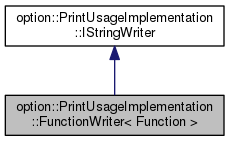
\includegraphics[width=244pt]{structoption_1_1PrintUsageImplementation_1_1FunctionWriter__inherit__graph}
\end{center}
\end{figure}


Collaboration diagram for option\+:\+:Print\+Usage\+Implementation\+:\+:Function\+Writer$<$ Function $>$\+:\nopagebreak
\begin{figure}[H]
\begin{center}
\leavevmode
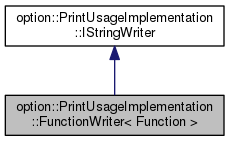
\includegraphics[width=244pt]{structoption_1_1PrintUsageImplementation_1_1FunctionWriter__coll__graph}
\end{center}
\end{figure}
\subsection*{Public Member Functions}
\begin{DoxyCompactItemize}
\item 
\mbox{\Hypertarget{structoption_1_1PrintUsageImplementation_1_1FunctionWriter_aa8e8f237845e210e36ca431d7e503a70}\label{structoption_1_1PrintUsageImplementation_1_1FunctionWriter_aa8e8f237845e210e36ca431d7e503a70}} 
virtual void \hyperlink{structoption_1_1PrintUsageImplementation_1_1FunctionWriter_aa8e8f237845e210e36ca431d7e503a70}{operator()} (const char $\ast$str, int size)
\begin{DoxyCompactList}\small\item\em Writes the given number of chars beginning at the given pointer somewhere. \end{DoxyCompactList}\item 
\mbox{\Hypertarget{structoption_1_1PrintUsageImplementation_1_1FunctionWriter_adc6c3f7ba11b3cad65c018955bab47e5}\label{structoption_1_1PrintUsageImplementation_1_1FunctionWriter_adc6c3f7ba11b3cad65c018955bab47e5}} 
{\bfseries Function\+Writer} (Function $\ast$w)
\end{DoxyCompactItemize}
\subsection*{Public Attributes}
\begin{DoxyCompactItemize}
\item 
\mbox{\Hypertarget{structoption_1_1PrintUsageImplementation_1_1FunctionWriter_a3442e05eb04d2b1ee321193f5b10557b}\label{structoption_1_1PrintUsageImplementation_1_1FunctionWriter_a3442e05eb04d2b1ee321193f5b10557b}} 
Function $\ast$ {\bfseries write}
\end{DoxyCompactItemize}


The documentation for this struct was generated from the following file\+:\begin{DoxyCompactItemize}
\item 
\hyperlink{optionparser_8h}{optionparser.\+h}\end{DoxyCompactItemize}

\hypertarget{classhebi_1_1Group}{}\section{hebi\+:\+:Group Class Reference}
\label{classhebi_1_1Group}\index{hebi\+::\+Group@{hebi\+::\+Group}}


Represents a group of physical H\+E\+BI modules, and allows \hyperlink{classhebi_1_1Command}{Command}, \hyperlink{classhebi_1_1Feedback}{Feedback}, and \hyperlink{classhebi_1_1Info}{Info} objects to be sent to and recieved from the hardware.  




{\ttfamily \#include $<$group.\+hpp$>$}

\subsection*{Public Member Functions}
\begin{DoxyCompactItemize}
\item 
\hyperlink{classhebi_1_1Group_a52041e4d07d6d0767c52bb896d125e84}{Group} (Hebi\+Group\+Ptr group)
\item 
\mbox{\Hypertarget{classhebi_1_1Group_affa9e3421af94d40a670112e53acaa1d}\label{classhebi_1_1Group_affa9e3421af94d40a670112e53acaa1d}} 
virtual \hyperlink{classhebi_1_1Group_affa9e3421af94d40a670112e53acaa1d}{$\sim$\+Group} () noexcept
\begin{DoxyCompactList}\small\item\em Destructor cleans up group. \end{DoxyCompactList}\item 
\mbox{\Hypertarget{classhebi_1_1Group_a3cc170c50e51cfc25bc73ae5680bd115}\label{classhebi_1_1Group_a3cc170c50e51cfc25bc73ae5680bd115}} 
int \hyperlink{classhebi_1_1Group_a3cc170c50e51cfc25bc73ae5680bd115}{size} ()
\begin{DoxyCompactList}\small\item\em Returns the number of modules in the group. \end{DoxyCompactList}\item 
bool \hyperlink{classhebi_1_1Group_a3645f8c1019e6949dc64fbdec7f73442}{send\+Command} (const \hyperlink{classhebi_1_1GroupCommand}{Group\+Command} \&group\+\_\+command)
\begin{DoxyCompactList}\small\item\em Send a command to the given group without requesting an acknowledgement. \end{DoxyCompactList}\item 
bool \hyperlink{classhebi_1_1Group_a992aad2873e2d108c2d4deb3f824a538}{send\+Command\+With\+Acknowledgement} (const \hyperlink{classhebi_1_1GroupCommand}{Group\+Command} \&group\+\_\+command, int timeout\+\_\+ms=\hyperlink{classhebi_1_1Group_a3d01ca6dbd28ec984cda196a77056dd4}{D\+E\+F\+A\+U\+L\+T\+\_\+\+T\+I\+M\+E\+O\+U\+T\+\_\+\+MS})
\begin{DoxyCompactList}\small\item\em Send a command to the given group, requesting an acknowledgement of transmission to be sent back. \end{DoxyCompactList}\item 
bool \hyperlink{classhebi_1_1Group_a191170df8c2b64e039063e89449b4587}{request\+Feedback} (\hyperlink{classhebi_1_1GroupFeedback}{Group\+Feedback} $\ast$feedback, int timeout\+\_\+ms=\hyperlink{classhebi_1_1Group_a3d01ca6dbd28ec984cda196a77056dd4}{D\+E\+F\+A\+U\+L\+T\+\_\+\+T\+I\+M\+E\+O\+U\+T\+\_\+\+MS})
\begin{DoxyCompactList}\small\item\em Request feedback from the group, and store it in the passed-\/in feedback object. \end{DoxyCompactList}\item 
bool \hyperlink{classhebi_1_1Group_a1065ad12a649d135758c1b6a95df650e}{request\+Info} (\hyperlink{classhebi_1_1GroupInfo}{Group\+Info} $\ast$info, int timeout\+\_\+ms=\hyperlink{classhebi_1_1Group_a3d01ca6dbd28ec984cda196a77056dd4}{D\+E\+F\+A\+U\+L\+T\+\_\+\+T\+I\+M\+E\+O\+U\+T\+\_\+\+MS})
\begin{DoxyCompactList}\small\item\em Request info from the group, and store it in the passed-\/in info object. \end{DoxyCompactList}\item 
bool \hyperlink{classhebi_1_1Group_ac3760e72c22a47f365e8c23d9a6dcfb7}{start\+Log} ()
\begin{DoxyCompactList}\small\item\em Starts log (stopping any active log). W\+A\+R\+N\+I\+NG\+: interface not yet stable! \end{DoxyCompactList}\item 
bool \hyperlink{classhebi_1_1Group_adbbbbe95f600cb2843c1b51281a74744}{stop\+Log} ()
\begin{DoxyCompactList}\small\item\em Stops any active log. W\+A\+R\+N\+I\+NG\+: interface not yet stable! \end{DoxyCompactList}\item 
bool \hyperlink{classhebi_1_1Group_a4c2dce41b42dc0d318e220098c4d05e4}{set\+Feedback\+Frequency\+Hz} (float frequency)
\begin{DoxyCompactList}\small\item\em Sets the frequency of the internal feedback request + callback thread. \end{DoxyCompactList}\item 
float \hyperlink{classhebi_1_1Group_a5f8e63952136f4d0fc3b847c838985b9}{get\+Feedback\+Frequency\+Hz} ()
\begin{DoxyCompactList}\small\item\em Gets the frequency of the internal feedback request + callback thread. \end{DoxyCompactList}\item 
\mbox{\Hypertarget{classhebi_1_1Group_a9b428b5d5cf774f0dddc3b50b5daf90e}\label{classhebi_1_1Group_a9b428b5d5cf774f0dddc3b50b5daf90e}} 
void \hyperlink{classhebi_1_1Group_a9b428b5d5cf774f0dddc3b50b5daf90e}{add\+Feedback\+Handler} (Group\+Feedback\+Handler handler)
\begin{DoxyCompactList}\small\item\em Adds a handler function to be called by the internal feedback request thread. \end{DoxyCompactList}\item 
\mbox{\Hypertarget{classhebi_1_1Group_a54c23fbada200539f7f0d84d97b40f9b}\label{classhebi_1_1Group_a54c23fbada200539f7f0d84d97b40f9b}} 
void \hyperlink{classhebi_1_1Group_a54c23fbada200539f7f0d84d97b40f9b}{clear\+Feedback\+Handlers} ()
\begin{DoxyCompactList}\small\item\em Removes all feedback handlers presently added. \end{DoxyCompactList}\end{DoxyCompactItemize}
\subsection*{Static Public Attributes}
\begin{DoxyCompactItemize}
\item 
\mbox{\Hypertarget{classhebi_1_1Group_a3d01ca6dbd28ec984cda196a77056dd4}\label{classhebi_1_1Group_a3d01ca6dbd28ec984cda196a77056dd4}} 
static const int \hyperlink{classhebi_1_1Group_a3d01ca6dbd28ec984cda196a77056dd4}{D\+E\+F\+A\+U\+L\+T\+\_\+\+T\+I\+M\+E\+O\+U\+T\+\_\+\+MS} = 500
\begin{DoxyCompactList}\small\item\em The default timeout for any send-\/with-\/acknowledgement or request operation is 500 ms. \end{DoxyCompactList}\end{DoxyCompactItemize}
\subsection*{Friends}
\begin{DoxyCompactItemize}
\item 
void \hyperlink{classhebi_1_1Group_a895e36298e0e77c27c644c4e3edea356}{callback\+Wrapper} (Hebi\+Group\+Feedback\+Ptr group\+\_\+feedback, void $\ast$user\+\_\+data)
\end{DoxyCompactItemize}


\subsection{Detailed Description}
Represents a group of physical H\+E\+BI modules, and allows \hyperlink{classhebi_1_1Command}{Command}, \hyperlink{classhebi_1_1Feedback}{Feedback}, and \hyperlink{classhebi_1_1Info}{Info} objects to be sent to and recieved from the hardware. 

\subsection{Constructor \& Destructor Documentation}
\mbox{\Hypertarget{classhebi_1_1Group_a52041e4d07d6d0767c52bb896d125e84}\label{classhebi_1_1Group_a52041e4d07d6d0767c52bb896d125e84}} 
\index{hebi\+::\+Group@{hebi\+::\+Group}!Group@{Group}}
\index{Group@{Group}!hebi\+::\+Group@{hebi\+::\+Group}}
\subsubsection{\texorpdfstring{Group()}{Group()}}
{\footnotesize\ttfamily hebi\+::\+Group\+::\+Group (\begin{DoxyParamCaption}\item[{Hebi\+Group\+Ptr}]{group }\end{DoxyParamCaption})}

Creates a group from the underlying C-\/style group object. This should only be called to create groups from the lookup class, not from user code! 

\subsection{Member Function Documentation}
\mbox{\Hypertarget{classhebi_1_1Group_a5f8e63952136f4d0fc3b847c838985b9}\label{classhebi_1_1Group_a5f8e63952136f4d0fc3b847c838985b9}} 
\index{hebi\+::\+Group@{hebi\+::\+Group}!get\+Feedback\+Frequency\+Hz@{get\+Feedback\+Frequency\+Hz}}
\index{get\+Feedback\+Frequency\+Hz@{get\+Feedback\+Frequency\+Hz}!hebi\+::\+Group@{hebi\+::\+Group}}
\subsubsection{\texorpdfstring{get\+Feedback\+Frequency\+Hz()}{getFeedbackFrequencyHz()}}
{\footnotesize\ttfamily float hebi\+::\+Group\+::get\+Feedback\+Frequency\+Hz (\begin{DoxyParamCaption}{ }\end{DoxyParamCaption})}



Gets the frequency of the internal feedback request + callback thread. 

\begin{DoxyReturn}{Returns}
The current feedback request loop frequency (in Hz). 
\end{DoxyReturn}
\mbox{\Hypertarget{classhebi_1_1Group_a191170df8c2b64e039063e89449b4587}\label{classhebi_1_1Group_a191170df8c2b64e039063e89449b4587}} 
\index{hebi\+::\+Group@{hebi\+::\+Group}!request\+Feedback@{request\+Feedback}}
\index{request\+Feedback@{request\+Feedback}!hebi\+::\+Group@{hebi\+::\+Group}}
\subsubsection{\texorpdfstring{request\+Feedback()}{requestFeedback()}}
{\footnotesize\ttfamily bool hebi\+::\+Group\+::request\+Feedback (\begin{DoxyParamCaption}\item[{\hyperlink{classhebi_1_1GroupFeedback}{Group\+Feedback} $\ast$}]{feedback,  }\item[{int}]{timeout\+\_\+ms = {\ttfamily \hyperlink{classhebi_1_1Group_a3d01ca6dbd28ec984cda196a77056dd4}{D\+E\+F\+A\+U\+L\+T\+\_\+\+T\+I\+M\+E\+O\+U\+T\+\_\+\+MS}} }\end{DoxyParamCaption})}



Request feedback from the group, and store it in the passed-\/in feedback object. 

\begin{DoxyReturn}{Returns}
true if the request was successful within the specified timeout; in this case \textquotesingle{}feedback\textquotesingle{} has been updated. Otherwise, returns false and does not update \textquotesingle{}feedback\textquotesingle{}. 
\end{DoxyReturn}
\mbox{\Hypertarget{classhebi_1_1Group_a1065ad12a649d135758c1b6a95df650e}\label{classhebi_1_1Group_a1065ad12a649d135758c1b6a95df650e}} 
\index{hebi\+::\+Group@{hebi\+::\+Group}!request\+Info@{request\+Info}}
\index{request\+Info@{request\+Info}!hebi\+::\+Group@{hebi\+::\+Group}}
\subsubsection{\texorpdfstring{request\+Info()}{requestInfo()}}
{\footnotesize\ttfamily bool hebi\+::\+Group\+::request\+Info (\begin{DoxyParamCaption}\item[{\hyperlink{classhebi_1_1GroupInfo}{Group\+Info} $\ast$}]{info,  }\item[{int}]{timeout\+\_\+ms = {\ttfamily \hyperlink{classhebi_1_1Group_a3d01ca6dbd28ec984cda196a77056dd4}{D\+E\+F\+A\+U\+L\+T\+\_\+\+T\+I\+M\+E\+O\+U\+T\+\_\+\+MS}} }\end{DoxyParamCaption})}



Request info from the group, and store it in the passed-\/in info object. 

\begin{DoxyReturn}{Returns}
true if the request was successful within the specified timeout; in this case \textquotesingle{}info\textquotesingle{} has been updated. Otherwise, returns false and does not update \textquotesingle{}info\textquotesingle{}. 
\end{DoxyReturn}
\mbox{\Hypertarget{classhebi_1_1Group_a3645f8c1019e6949dc64fbdec7f73442}\label{classhebi_1_1Group_a3645f8c1019e6949dc64fbdec7f73442}} 
\index{hebi\+::\+Group@{hebi\+::\+Group}!send\+Command@{send\+Command}}
\index{send\+Command@{send\+Command}!hebi\+::\+Group@{hebi\+::\+Group}}
\subsubsection{\texorpdfstring{send\+Command()}{sendCommand()}}
{\footnotesize\ttfamily bool hebi\+::\+Group\+::send\+Command (\begin{DoxyParamCaption}\item[{const \hyperlink{classhebi_1_1GroupCommand}{Group\+Command} \&}]{group\+\_\+command }\end{DoxyParamCaption})}



Send a command to the given group without requesting an acknowledgement. 

Appropriate for high-\/frequency applications.


\begin{DoxyParams}{Parameters}
{\em command} & The \hyperlink{classhebi_1_1GroupCommand}{Group\+Command} object containing information to be sent to the group.\\
\hline
\end{DoxyParams}
\begin{DoxyReturn}{Returns}
true if the command was successfully sent, false otherwise. 
\end{DoxyReturn}
\mbox{\Hypertarget{classhebi_1_1Group_a992aad2873e2d108c2d4deb3f824a538}\label{classhebi_1_1Group_a992aad2873e2d108c2d4deb3f824a538}} 
\index{hebi\+::\+Group@{hebi\+::\+Group}!send\+Command\+With\+Acknowledgement@{send\+Command\+With\+Acknowledgement}}
\index{send\+Command\+With\+Acknowledgement@{send\+Command\+With\+Acknowledgement}!hebi\+::\+Group@{hebi\+::\+Group}}
\subsubsection{\texorpdfstring{send\+Command\+With\+Acknowledgement()}{sendCommandWithAcknowledgement()}}
{\footnotesize\ttfamily bool hebi\+::\+Group\+::send\+Command\+With\+Acknowledgement (\begin{DoxyParamCaption}\item[{const \hyperlink{classhebi_1_1GroupCommand}{Group\+Command} \&}]{group\+\_\+command,  }\item[{int}]{timeout\+\_\+ms = {\ttfamily \hyperlink{classhebi_1_1Group_a3d01ca6dbd28ec984cda196a77056dd4}{D\+E\+F\+A\+U\+L\+T\+\_\+\+T\+I\+M\+E\+O\+U\+T\+\_\+\+MS}} }\end{DoxyParamCaption})}



Send a command to the given group, requesting an acknowledgement of transmission to be sent back. 


\begin{DoxyParams}{Parameters}
{\em command} & The \hyperlink{classhebi_1_1GroupCommand}{Group\+Command} object containing information to be sent to the group. \\
\hline
{\em timeout\+\_\+ms} & Indicates how many milliseconds to wait for a response after sending a packet. For typical networks, \textquotesingle{}15\textquotesingle{} ms is a value that can be reasonably expected to encompass the time required for a round-\/trip transmission.\\
\hline
\end{DoxyParams}
\begin{DoxyReturn}{Returns}
true if an acknowledgement was successfully received (guaranteeing the group received this command), or a negative number for an error otherwise.
\end{DoxyReturn}
Note\+: A non-\/true return does not indicate a specific failure, and may result from an error while sending or simply a timeout/dropped response packet after a successful transmission. \mbox{\Hypertarget{classhebi_1_1Group_a4c2dce41b42dc0d318e220098c4d05e4}\label{classhebi_1_1Group_a4c2dce41b42dc0d318e220098c4d05e4}} 
\index{hebi\+::\+Group@{hebi\+::\+Group}!set\+Feedback\+Frequency\+Hz@{set\+Feedback\+Frequency\+Hz}}
\index{set\+Feedback\+Frequency\+Hz@{set\+Feedback\+Frequency\+Hz}!hebi\+::\+Group@{hebi\+::\+Group}}
\subsubsection{\texorpdfstring{set\+Feedback\+Frequency\+Hz()}{setFeedbackFrequencyHz()}}
{\footnotesize\ttfamily bool hebi\+::\+Group\+::set\+Feedback\+Frequency\+Hz (\begin{DoxyParamCaption}\item[{float}]{frequency }\end{DoxyParamCaption})}



Sets the frequency of the internal feedback request + callback thread. 

\begin{DoxyReturn}{Returns}
{\ttfamily true} if the frequency successfully was set, or {\ttfamily false} if the parameter was outside the accepted range (less than zero or faster than supported maximum). 
\end{DoxyReturn}
\mbox{\Hypertarget{classhebi_1_1Group_ac3760e72c22a47f365e8c23d9a6dcfb7}\label{classhebi_1_1Group_ac3760e72c22a47f365e8c23d9a6dcfb7}} 
\index{hebi\+::\+Group@{hebi\+::\+Group}!start\+Log@{start\+Log}}
\index{start\+Log@{start\+Log}!hebi\+::\+Group@{hebi\+::\+Group}}
\subsubsection{\texorpdfstring{start\+Log()}{startLog()}}
{\footnotesize\ttfamily bool hebi\+::\+Group\+::start\+Log (\begin{DoxyParamCaption}{ }\end{DoxyParamCaption})}



Starts log (stopping any active log). W\+A\+R\+N\+I\+NG\+: interface not yet stable! 

N\+O\+TE\+: E\+X\+P\+E\+R\+I\+M\+E\+N\+T\+AL U\+SE O\+N\+LY -\/ F\+U\+N\+C\+T\+I\+ON I\+N\+T\+E\+R\+F\+A\+CE S\+U\+B\+J\+E\+CT TO C\+H\+A\+N\+GE.

\begin{DoxyReturn}{Returns}
true on success. 
\end{DoxyReturn}
\mbox{\Hypertarget{classhebi_1_1Group_adbbbbe95f600cb2843c1b51281a74744}\label{classhebi_1_1Group_adbbbbe95f600cb2843c1b51281a74744}} 
\index{hebi\+::\+Group@{hebi\+::\+Group}!stop\+Log@{stop\+Log}}
\index{stop\+Log@{stop\+Log}!hebi\+::\+Group@{hebi\+::\+Group}}
\subsubsection{\texorpdfstring{stop\+Log()}{stopLog()}}
{\footnotesize\ttfamily bool hebi\+::\+Group\+::stop\+Log (\begin{DoxyParamCaption}{ }\end{DoxyParamCaption})}



Stops any active log. W\+A\+R\+N\+I\+NG\+: interface not yet stable! 

N\+O\+TE\+: E\+X\+P\+E\+R\+I\+M\+E\+N\+T\+AL U\+SE O\+N\+LY -\/ F\+U\+N\+C\+T\+I\+ON I\+N\+T\+E\+R\+F\+A\+CE S\+U\+B\+J\+E\+CT TO C\+H\+A\+N\+GE.

\begin{DoxyReturn}{Returns}
true if a log was running and was successfully stopped, false otherwise. 
\end{DoxyReturn}


\subsection{Friends And Related Function Documentation}
\mbox{\Hypertarget{classhebi_1_1Group_a895e36298e0e77c27c644c4e3edea356}\label{classhebi_1_1Group_a895e36298e0e77c27c644c4e3edea356}} 
\index{hebi\+::\+Group@{hebi\+::\+Group}!callback\+Wrapper@{callback\+Wrapper}}
\index{callback\+Wrapper@{callback\+Wrapper}!hebi\+::\+Group@{hebi\+::\+Group}}
\subsubsection{\texorpdfstring{callback\+Wrapper}{callbackWrapper}}
{\footnotesize\ttfamily void callback\+Wrapper (\begin{DoxyParamCaption}\item[{Hebi\+Group\+Feedback\+Ptr}]{group\+\_\+feedback,  }\item[{void $\ast$}]{user\+\_\+data }\end{DoxyParamCaption})\hspace{0.3cm}{\ttfamily [friend]}}

Intermediary to convert C-\/style function callbacks to C++ style, and change callback parameter types. 

The documentation for this class was generated from the following files\+:\begin{DoxyCompactItemize}
\item 
group.\+hpp\item 
group.\+cpp\end{DoxyCompactItemize}

\hypertarget{classhebi_1_1GroupCommand}{}\section{hebi\+:\+:Group\+Command Class Reference}
\label{classhebi_1_1GroupCommand}\index{hebi\+::\+Group\+Command@{hebi\+::\+Group\+Command}}


A list of \hyperlink{classhebi_1_1Command}{Command} objects appropriate for sending to a \hyperlink{classhebi_1_1Group}{Group} of modules; the \hyperlink{classhebi_1_1GroupCommand_a75645b28175dde77de35801909d58213}{size()} must match the number of modules in the group.  




{\ttfamily \#include $<$group\+\_\+command.\+hpp$>$}

\subsection*{Public Member Functions}
\begin{DoxyCompactItemize}
\item 
\hyperlink{classhebi_1_1GroupCommand_a7a41c0aace3d99b0d7e9dcd9b1063a11}{Group\+Command} (int number\+\_\+of\+\_\+modules)\hypertarget{classhebi_1_1GroupCommand_a7a41c0aace3d99b0d7e9dcd9b1063a11}{}\label{classhebi_1_1GroupCommand_a7a41c0aace3d99b0d7e9dcd9b1063a11}

\begin{DoxyCompactList}\small\item\em Create a group command with the specified number of modules. \end{DoxyCompactList}\item 
virtual \hyperlink{classhebi_1_1GroupCommand_a382b2ce9d36ab4892a5191407001455c}{$\sim$\+Group\+Command} () noexcept\hypertarget{classhebi_1_1GroupCommand_a382b2ce9d36ab4892a5191407001455c}{}\label{classhebi_1_1GroupCommand_a382b2ce9d36ab4892a5191407001455c}

\begin{DoxyCompactList}\small\item\em Destructor cleans up group command object as necessary. \end{DoxyCompactList}\item 
int \hyperlink{classhebi_1_1GroupCommand_a75645b28175dde77de35801909d58213}{size} () const \hypertarget{classhebi_1_1GroupCommand_a75645b28175dde77de35801909d58213}{}\label{classhebi_1_1GroupCommand_a75645b28175dde77de35801909d58213}

\begin{DoxyCompactList}\small\item\em Returns the number of module commands in this group command. \end{DoxyCompactList}\item 
\hyperlink{classhebi_1_1Command}{Command} \& \hyperlink{classhebi_1_1GroupCommand_afa9edb2ec0c411b4d9ca701350339a90}{operator\mbox{[}$\,$\mbox{]}} (int index)
\end{DoxyCompactItemize}
\subsection*{Public Attributes}
\begin{DoxyCompactItemize}
\item 
Hebi\+Group\+Command\+Ptr const \hyperlink{classhebi_1_1GroupCommand_aa3380b0b6c64b2d03df3d5d69a884a12}{internal\+\_\+}
\end{DoxyCompactItemize}


\subsection{Detailed Description}
A list of \hyperlink{classhebi_1_1Command}{Command} objects appropriate for sending to a \hyperlink{classhebi_1_1Group}{Group} of modules; the \hyperlink{classhebi_1_1GroupCommand_a75645b28175dde77de35801909d58213}{size()} must match the number of modules in the group. 

\subsection{Member Function Documentation}
\index{hebi\+::\+Group\+Command@{hebi\+::\+Group\+Command}!operator\mbox{[}$\,$\mbox{]}@{operator[]}}
\index{operator\mbox{[}$\,$\mbox{]}@{operator[]}!hebi\+::\+Group\+Command@{hebi\+::\+Group\+Command}}
\subsubsection[{\texorpdfstring{operator[](int index)}{operator[](int index)}}]{\setlength{\rightskip}{0pt plus 5cm}{\bf Command} \& hebi\+::\+Group\+Command\+::operator\mbox{[}$\,$\mbox{]} (
\begin{DoxyParamCaption}
\item[{int}]{index}
\end{DoxyParamCaption}
)}\hypertarget{classhebi_1_1GroupCommand_afa9edb2ec0c411b4d9ca701350339a90}{}\label{classhebi_1_1GroupCommand_afa9edb2ec0c411b4d9ca701350339a90}
brief Access the command for an individual module. 

\subsection{Member Data Documentation}
\index{hebi\+::\+Group\+Command@{hebi\+::\+Group\+Command}!internal\+\_\+@{internal\+\_\+}}
\index{internal\+\_\+@{internal\+\_\+}!hebi\+::\+Group\+Command@{hebi\+::\+Group\+Command}}
\subsubsection[{\texorpdfstring{internal\+\_\+}{internal_}}]{\setlength{\rightskip}{0pt plus 5cm}Hebi\+Group\+Command\+Ptr const hebi\+::\+Group\+Command\+::internal\+\_\+}\hypertarget{classhebi_1_1GroupCommand_aa3380b0b6c64b2d03df3d5d69a884a12}{}\label{classhebi_1_1GroupCommand_aa3380b0b6c64b2d03df3d5d69a884a12}
C-\/style group command object. N\+O\+TE\+: this should not be used except by library functions! 

The documentation for this class was generated from the following files\+:\begin{DoxyCompactItemize}
\item 
group\+\_\+command.\+hpp\item 
group\+\_\+command.\+cpp\end{DoxyCompactItemize}

\hypertarget{classhebi_1_1GroupFeedback}{}\section{hebi\+:\+:Group\+Feedback Class Reference}
\label{classhebi_1_1GroupFeedback}\index{hebi\+::\+Group\+Feedback@{hebi\+::\+Group\+Feedback}}


A list of \hyperlink{classhebi_1_1Feedback}{Feedback} objects that can be received from a \hyperlink{classhebi_1_1Group}{Group} of modules; the \hyperlink{classhebi_1_1GroupFeedback_a7509084e361feaf90d857d77afa4e4c0}{size()} must match the number of modules in the group.  




{\ttfamily \#include $<$group\+\_\+feedback.\+hpp$>$}

\subsection*{Public Member Functions}
\begin{DoxyCompactItemize}
\item 
\mbox{\Hypertarget{classhebi_1_1GroupFeedback_af0a41119c345d68c6ae390ff39be77fc}\label{classhebi_1_1GroupFeedback_af0a41119c345d68c6ae390ff39be77fc}} 
\hyperlink{classhebi_1_1GroupFeedback_af0a41119c345d68c6ae390ff39be77fc}{Group\+Feedback} (int number\+\_\+of\+\_\+modules)
\begin{DoxyCompactList}\small\item\em Create a group feedback with the specified number of modules. \end{DoxyCompactList}\item 
\hyperlink{classhebi_1_1GroupFeedback_ac12b1f1320eb14943d1b2600b0eecb1b}{Group\+Feedback} (Hebi\+Group\+Feedback\+Ptr group\+\_\+feedback)
\item 
\mbox{\Hypertarget{classhebi_1_1GroupFeedback_aef61ac5e6ac95a4c981cb6fc2d461d5f}\label{classhebi_1_1GroupFeedback_aef61ac5e6ac95a4c981cb6fc2d461d5f}} 
virtual \hyperlink{classhebi_1_1GroupFeedback_aef61ac5e6ac95a4c981cb6fc2d461d5f}{$\sim$\+Group\+Feedback} () noexcept
\begin{DoxyCompactList}\small\item\em Destructor cleans up group feedback object as necessary. \end{DoxyCompactList}\item 
\mbox{\Hypertarget{classhebi_1_1GroupFeedback_a7509084e361feaf90d857d77afa4e4c0}\label{classhebi_1_1GroupFeedback_a7509084e361feaf90d857d77afa4e4c0}} 
int \hyperlink{classhebi_1_1GroupFeedback_a7509084e361feaf90d857d77afa4e4c0}{size} () const
\begin{DoxyCompactList}\small\item\em Returns the number of module feedbacks in this group feedback. \end{DoxyCompactList}\item 
\mbox{\Hypertarget{classhebi_1_1GroupFeedback_a4043d1389b921deec5613736c8d36460}\label{classhebi_1_1GroupFeedback_a4043d1389b921deec5613736c8d36460}} 
const \hyperlink{classhebi_1_1Feedback}{Feedback} \& \hyperlink{classhebi_1_1GroupFeedback_a4043d1389b921deec5613736c8d36460}{operator\mbox{[}$\,$\mbox{]}} (int index) const
\begin{DoxyCompactList}\small\item\em Access the feedback for an individual module. \end{DoxyCompactList}\end{DoxyCompactItemize}
\subsection*{Public Attributes}
\begin{DoxyCompactItemize}
\item 
Hebi\+Group\+Feedback\+Ptr const \hyperlink{classhebi_1_1GroupFeedback_ac549a7728905ca72e5a19256afaf9d49}{internal\+\_\+}
\end{DoxyCompactItemize}


\subsection{Detailed Description}
A list of \hyperlink{classhebi_1_1Feedback}{Feedback} objects that can be received from a \hyperlink{classhebi_1_1Group}{Group} of modules; the \hyperlink{classhebi_1_1GroupFeedback_a7509084e361feaf90d857d77afa4e4c0}{size()} must match the number of modules in the group. 

\subsection{Constructor \& Destructor Documentation}
\mbox{\Hypertarget{classhebi_1_1GroupFeedback_ac12b1f1320eb14943d1b2600b0eecb1b}\label{classhebi_1_1GroupFeedback_ac12b1f1320eb14943d1b2600b0eecb1b}} 
\index{hebi\+::\+Group\+Feedback@{hebi\+::\+Group\+Feedback}!Group\+Feedback@{Group\+Feedback}}
\index{Group\+Feedback@{Group\+Feedback}!hebi\+::\+Group\+Feedback@{hebi\+::\+Group\+Feedback}}
\subsubsection{\texorpdfstring{Group\+Feedback()}{GroupFeedback()}}
{\footnotesize\ttfamily hebi\+::\+Group\+Feedback\+::\+Group\+Feedback (\begin{DoxyParamCaption}\item[{Hebi\+Group\+Feedback\+Ptr}]{group\+\_\+feedback }\end{DoxyParamCaption})}

Wraps an existing C-\/style feedback object; object lifetime is assumed to be managed by the caller. N\+O\+TE\+: this should not be used except by internal library functions! 

\subsection{Member Data Documentation}
\mbox{\Hypertarget{classhebi_1_1GroupFeedback_ac549a7728905ca72e5a19256afaf9d49}\label{classhebi_1_1GroupFeedback_ac549a7728905ca72e5a19256afaf9d49}} 
\index{hebi\+::\+Group\+Feedback@{hebi\+::\+Group\+Feedback}!internal\+\_\+@{internal\+\_\+}}
\index{internal\+\_\+@{internal\+\_\+}!hebi\+::\+Group\+Feedback@{hebi\+::\+Group\+Feedback}}
\subsubsection{\texorpdfstring{internal\+\_\+}{internal\_}}
{\footnotesize\ttfamily Hebi\+Group\+Feedback\+Ptr const hebi\+::\+Group\+Feedback\+::internal\+\_\+}

C-\/style group feedback object. N\+O\+TE\+: this should not be used except by library functions! 

The documentation for this class was generated from the following files\+:\begin{DoxyCompactItemize}
\item 
group\+\_\+feedback.\+hpp\item 
group\+\_\+feedback.\+cpp\end{DoxyCompactItemize}

\hypertarget{classhebi_1_1GroupInfo}{}\section{hebi\+:\+:Group\+Info Class Reference}
\label{classhebi_1_1GroupInfo}\index{hebi\+::\+Group\+Info@{hebi\+::\+Group\+Info}}


A list of \hyperlink{classhebi_1_1Info}{Info} objects that can be received from a \hyperlink{classhebi_1_1Group}{Group} of modules; the \hyperlink{classhebi_1_1GroupInfo_a197165d1017e42ebbf4f9c527bb1b706}{size()} must match the number of modules in the group.  




{\ttfamily \#include $<$group\+\_\+info.\+hpp$>$}

\subsection*{Public Member Functions}
\begin{DoxyCompactItemize}
\item 
\hyperlink{classhebi_1_1GroupInfo_adb2618d3baaadb15328d04427e64d9fc}{Group\+Info} (int number\+\_\+of\+\_\+modules)\hypertarget{classhebi_1_1GroupInfo_adb2618d3baaadb15328d04427e64d9fc}{}\label{classhebi_1_1GroupInfo_adb2618d3baaadb15328d04427e64d9fc}

\begin{DoxyCompactList}\small\item\em Create a group info with the specified number of modules. \end{DoxyCompactList}\item 
virtual \hyperlink{classhebi_1_1GroupInfo_a2bdd19dd45afff8c0d6a3e212f0a75e6}{$\sim$\+Group\+Info} () noexcept\hypertarget{classhebi_1_1GroupInfo_a2bdd19dd45afff8c0d6a3e212f0a75e6}{}\label{classhebi_1_1GroupInfo_a2bdd19dd45afff8c0d6a3e212f0a75e6}

\begin{DoxyCompactList}\small\item\em Destructor cleans up group info object as necessary. \end{DoxyCompactList}\item 
int \hyperlink{classhebi_1_1GroupInfo_a197165d1017e42ebbf4f9c527bb1b706}{size} () const \hypertarget{classhebi_1_1GroupInfo_a197165d1017e42ebbf4f9c527bb1b706}{}\label{classhebi_1_1GroupInfo_a197165d1017e42ebbf4f9c527bb1b706}

\begin{DoxyCompactList}\small\item\em Returns the number of module infos in this group info. \end{DoxyCompactList}\item 
const \hyperlink{classhebi_1_1Info}{Info} \& \hyperlink{classhebi_1_1GroupInfo_a3b1fed2ae8cefc7306a07fd39aab3a2f}{operator\mbox{[}$\,$\mbox{]}} (int index) const \hypertarget{classhebi_1_1GroupInfo_a3b1fed2ae8cefc7306a07fd39aab3a2f}{}\label{classhebi_1_1GroupInfo_a3b1fed2ae8cefc7306a07fd39aab3a2f}

\begin{DoxyCompactList}\small\item\em Access the info for an individual module. \end{DoxyCompactList}\end{DoxyCompactItemize}
\subsection*{Public Attributes}
\begin{DoxyCompactItemize}
\item 
Hebi\+Group\+Info\+Ptr const \hyperlink{classhebi_1_1GroupInfo_a35246a60a176870a343eb109e85fcfdf}{internal\+\_\+}
\end{DoxyCompactItemize}


\subsection{Detailed Description}
A list of \hyperlink{classhebi_1_1Info}{Info} objects that can be received from a \hyperlink{classhebi_1_1Group}{Group} of modules; the \hyperlink{classhebi_1_1GroupInfo_a197165d1017e42ebbf4f9c527bb1b706}{size()} must match the number of modules in the group. 

\subsection{Member Data Documentation}
\index{hebi\+::\+Group\+Info@{hebi\+::\+Group\+Info}!internal\+\_\+@{internal\+\_\+}}
\index{internal\+\_\+@{internal\+\_\+}!hebi\+::\+Group\+Info@{hebi\+::\+Group\+Info}}
\subsubsection[{\texorpdfstring{internal\+\_\+}{internal_}}]{\setlength{\rightskip}{0pt plus 5cm}Hebi\+Group\+Info\+Ptr const hebi\+::\+Group\+Info\+::internal\+\_\+}\hypertarget{classhebi_1_1GroupInfo_a35246a60a176870a343eb109e85fcfdf}{}\label{classhebi_1_1GroupInfo_a35246a60a176870a343eb109e85fcfdf}
C-\/style group info object. N\+O\+TE\+: this should not be used except by library functions! 

The documentation for this class was generated from the following files\+:\begin{DoxyCompactItemize}
\item 
group\+\_\+info.\+hpp\item 
group\+\_\+info.\+cpp\end{DoxyCompactItemize}

\hypertarget{classhebiSub}{}\section{hebi\+Sub Class Reference}
\label{classhebiSub}\index{hebi\+Sub@{hebi\+Sub}}
\subsection*{Public Member Functions}
\begin{DoxyCompactItemize}
\item 
\mbox{\Hypertarget{classhebiSub_a4318a55cd9c3d04e707d4f967ce3fa8b}\label{classhebiSub_a4318a55cd9c3d04e707d4f967ce3fa8b}} 
{\bfseries hebi\+Sub} (int)
\item 
\mbox{\Hypertarget{classhebiSub_a138b3fb698f64019f9066b6e22793cc4}\label{classhebiSub_a138b3fb698f64019f9066b6e22793cc4}} 
void {\bfseries hebi\+Callback} (const std\+\_\+msgs\+::\+Float32\+Multi\+Array\+::\+Const\+Ptr \&)
\end{DoxyCompactItemize}
\subsection*{Public Attributes}
\begin{DoxyCompactItemize}
\item 
\mbox{\Hypertarget{classhebiSub_ab121e7d471d3a847d24b319eadca516b}\label{classhebiSub_ab121e7d471d3a847d24b319eadca516b}} 
std\+::vector$<$ std\+\_\+msgs\+::\+Float32 $>$ {\bfseries position\+\_\+cmd}
\item 
\mbox{\Hypertarget{classhebiSub_add86ca7606f19981d627f881103ba6bd}\label{classhebiSub_add86ca7606f19981d627f881103ba6bd}} 
int {\bfseries n\+\_\+mod}
\end{DoxyCompactItemize}


The documentation for this class was generated from the following file\+:\begin{DoxyCompactItemize}
\item 
hebi\+\_\+listener.\+cpp\end{DoxyCompactItemize}

\hypertarget{classhebi_1_1Command_1_1HighResAngleField}{}\section{hebi\+:\+:Command\+:\+:High\+Res\+Angle\+Field Class Reference}
\label{classhebi_1_1Command_1_1HighResAngleField}\index{hebi\+::\+Command\+::\+High\+Res\+Angle\+Field@{hebi\+::\+Command\+::\+High\+Res\+Angle\+Field}}


A message field for an angle measurement which does not lose precision at very high angles.  




{\ttfamily \#include $<$command.\+hpp$>$}

\subsection*{Public Member Functions}
\begin{DoxyCompactItemize}
\item 
{\bfseries High\+Res\+Angle\+Field} (Hebi\+Command\+Ptr internal, Command\+High\+Res\+Angle\+Field field)\hypertarget{classhebi_1_1Command_1_1HighResAngleField_aaf8bed01fb55cacfc0d2e9965469c8f0}{}\label{classhebi_1_1Command_1_1HighResAngleField_aaf8bed01fb55cacfc0d2e9965469c8f0}

\item 
\hyperlink{classhebi_1_1Command_1_1HighResAngleField_a2cc4e740bd11af44140a446164b49d81}{operator bool} () const 
\begin{DoxyCompactList}\small\item\em Allows casting to a bool to check if the field has a value without directly calling {\ttfamily \hyperlink{classhebi_1_1Command_1_1HighResAngleField_aa8015d3d55a4205021f42a354e2b84a9}{has()}}. \end{DoxyCompactList}\item 
bool \hyperlink{classhebi_1_1Command_1_1HighResAngleField_aa8015d3d55a4205021f42a354e2b84a9}{has} () const \hypertarget{classhebi_1_1Command_1_1HighResAngleField_aa8015d3d55a4205021f42a354e2b84a9}{}\label{classhebi_1_1Command_1_1HighResAngleField_aa8015d3d55a4205021f42a354e2b84a9}

\begin{DoxyCompactList}\small\item\em True if (and only if) the field has a value. \end{DoxyCompactList}\item 
double \hyperlink{classhebi_1_1Command_1_1HighResAngleField_aa6be447c47691c4f1d5edb3797a99025}{get} () const 
\begin{DoxyCompactList}\small\item\em If the field has a value, returns that value as a double; otherwise, returns a default. \end{DoxyCompactList}\item 
void \hyperlink{classhebi_1_1Command_1_1HighResAngleField_ac00b4014c5b81ce1e44da92bb5989953}{get} (int64\+\_\+t $\ast$revolutions, float $\ast$radian\+\_\+offset) const 
\begin{DoxyCompactList}\small\item\em If the field has a value, returns that value in the int64 and float parameters passed in; otherwise, returns a default. \end{DoxyCompactList}\item 
void \hyperlink{classhebi_1_1Command_1_1HighResAngleField_aa166a76f8a6ea47b62dd53bee853fe90}{set} (double radians)\hypertarget{classhebi_1_1Command_1_1HighResAngleField_aa166a76f8a6ea47b62dd53bee853fe90}{}\label{classhebi_1_1Command_1_1HighResAngleField_aa166a76f8a6ea47b62dd53bee853fe90}

\begin{DoxyCompactList}\small\item\em Sets the field to a given double value (in radians). Note that double precision floating point numbers cannot represent the same angular resolution at very high magnitudes as they can at lower magnitudes. \end{DoxyCompactList}\item 
void \hyperlink{classhebi_1_1Command_1_1HighResAngleField_ad70b3a6cb991a2096466fb04d3973429}{set} (int64\+\_\+t revolutions, float radian\+\_\+offset)\hypertarget{classhebi_1_1Command_1_1HighResAngleField_ad70b3a6cb991a2096466fb04d3973429}{}\label{classhebi_1_1Command_1_1HighResAngleField_ad70b3a6cb991a2096466fb04d3973429}

\begin{DoxyCompactList}\small\item\em Sets the field to a given integer number of revolutions and a floating point offset from this number of revolutions. The offset does not specifically need to fall within a certain range (i.\+e., can add more than a single revolution to the integer value), but should be kept relatively small (e.\+g., below 10,000) to avoid potential loss of precision. \end{DoxyCompactList}\item 
void \hyperlink{classhebi_1_1Command_1_1HighResAngleField_a2a7485482fbf0311d992c0db4036d5c1}{clear} ()\hypertarget{classhebi_1_1Command_1_1HighResAngleField_a2a7485482fbf0311d992c0db4036d5c1}{}\label{classhebi_1_1Command_1_1HighResAngleField_a2a7485482fbf0311d992c0db4036d5c1}

\begin{DoxyCompactList}\small\item\em Removes any currently set value for this field. \end{DoxyCompactList}\end{DoxyCompactItemize}


\subsection{Detailed Description}
A message field for an angle measurement which does not lose precision at very high angles. 

This field is represented as an int64\+\_\+t for the number of revolutions and a float for the radian offset from that number of revolutions. 

\subsection{Member Function Documentation}
\index{hebi\+::\+Command\+::\+High\+Res\+Angle\+Field@{hebi\+::\+Command\+::\+High\+Res\+Angle\+Field}!get@{get}}
\index{get@{get}!hebi\+::\+Command\+::\+High\+Res\+Angle\+Field@{hebi\+::\+Command\+::\+High\+Res\+Angle\+Field}}
\subsubsection[{\texorpdfstring{get() const }{get() const }}]{\setlength{\rightskip}{0pt plus 5cm}double hebi\+::\+Command\+::\+High\+Res\+Angle\+Field\+::get (
\begin{DoxyParamCaption}
{}
\end{DoxyParamCaption}
) const}\hypertarget{classhebi_1_1Command_1_1HighResAngleField_aa6be447c47691c4f1d5edb3797a99025}{}\label{classhebi_1_1Command_1_1HighResAngleField_aa6be447c47691c4f1d5edb3797a99025}


If the field has a value, returns that value as a double; otherwise, returns a default. 

Note that some precision might be lost converting to a double at very high number of revolutions. \index{hebi\+::\+Command\+::\+High\+Res\+Angle\+Field@{hebi\+::\+Command\+::\+High\+Res\+Angle\+Field}!get@{get}}
\index{get@{get}!hebi\+::\+Command\+::\+High\+Res\+Angle\+Field@{hebi\+::\+Command\+::\+High\+Res\+Angle\+Field}}
\subsubsection[{\texorpdfstring{get(int64\+\_\+t $\ast$revolutions, float $\ast$radian\+\_\+offset) const }{get(int64_t *revolutions, float *radian_offset) const }}]{\setlength{\rightskip}{0pt plus 5cm}void hebi\+::\+Command\+::\+High\+Res\+Angle\+Field\+::get (
\begin{DoxyParamCaption}
\item[{int64\+\_\+t $\ast$}]{revolutions, }
\item[{float $\ast$}]{radian\+\_\+offset}
\end{DoxyParamCaption}
) const}\hypertarget{classhebi_1_1Command_1_1HighResAngleField_ac00b4014c5b81ce1e44da92bb5989953}{}\label{classhebi_1_1Command_1_1HighResAngleField_ac00b4014c5b81ce1e44da92bb5989953}


If the field has a value, returns that value in the int64 and float parameters passed in; otherwise, returns a default. 

Note that this maintains the full precision of the underlying angle measurement, even for very large numbers of revolutions.


\begin{DoxyParams}{Parameters}
{\em revolutions} & The number of full revolutions\\
\hline
{\em radian\+\_\+offset} & The offset from the given number of full revolutions. Note that this is usually between 0 and {\ttfamily 2$\ast$\+M\+\_\+\+PI}, but callers should not assume this. \\
\hline
\end{DoxyParams}
\index{hebi\+::\+Command\+::\+High\+Res\+Angle\+Field@{hebi\+::\+Command\+::\+High\+Res\+Angle\+Field}!operator bool@{operator bool}}
\index{operator bool@{operator bool}!hebi\+::\+Command\+::\+High\+Res\+Angle\+Field@{hebi\+::\+Command\+::\+High\+Res\+Angle\+Field}}
\subsubsection[{\texorpdfstring{operator bool() const }{operator bool() const }}]{\setlength{\rightskip}{0pt plus 5cm}hebi\+::\+Command\+::\+High\+Res\+Angle\+Field\+::operator bool (
\begin{DoxyParamCaption}
{}
\end{DoxyParamCaption}
) const\hspace{0.3cm}{\ttfamily [explicit]}}\hypertarget{classhebi_1_1Command_1_1HighResAngleField_a2cc4e740bd11af44140a446164b49d81}{}\label{classhebi_1_1Command_1_1HighResAngleField_a2cc4e740bd11af44140a446164b49d81}


Allows casting to a bool to check if the field has a value without directly calling {\ttfamily \hyperlink{classhebi_1_1Command_1_1HighResAngleField_aa8015d3d55a4205021f42a354e2b84a9}{has()}}. 

This can be used as in the following (assuming \textquotesingle{}parent\textquotesingle{} is a parent message, and this field is called \textquotesingle{}my\+Field\textquotesingle{}) 
\begin{DoxyCode}
Command::HighResAngleField& f = parent.myField();
\textcolor{keywordflow}{if} (f)
  std::cout << \textcolor{stringliteral}{"Field has value: "} << f.get() << std::endl;
\textcolor{keywordflow}{else}
  std::cout << \textcolor{stringliteral}{"Field has no value!"} << std::endl;
\end{DoxyCode}
 

The documentation for this class was generated from the following files\+:\begin{DoxyCompactItemize}
\item 
command.\+hpp\item 
command.\+cpp\end{DoxyCompactItemize}

\hypertarget{classhebi_1_1Feedback_1_1HighResAngleField}{}\section{hebi\+:\+:Feedback\+:\+:High\+Res\+Angle\+Field Class Reference}
\label{classhebi_1_1Feedback_1_1HighResAngleField}\index{hebi\+::\+Feedback\+::\+High\+Res\+Angle\+Field@{hebi\+::\+Feedback\+::\+High\+Res\+Angle\+Field}}


A message field for an angle measurement which does not lose precision at very high angles.  




{\ttfamily \#include $<$feedback.\+hpp$>$}

\subsection*{Public Member Functions}
\begin{DoxyCompactItemize}
\item 
{\bfseries High\+Res\+Angle\+Field} (Hebi\+Feedback\+Ptr internal, Feedback\+High\+Res\+Angle\+Field field)\hypertarget{classhebi_1_1Feedback_1_1HighResAngleField_a58cd10f4e873eff00070789de04bcaf2}{}\label{classhebi_1_1Feedback_1_1HighResAngleField_a58cd10f4e873eff00070789de04bcaf2}

\item 
\hyperlink{classhebi_1_1Feedback_1_1HighResAngleField_a0e5b3a62cbebf87fab67c6b2472a0c95}{operator bool} () const 
\begin{DoxyCompactList}\small\item\em Allows casting to a bool to check if the field has a value without directly calling {\ttfamily \hyperlink{classhebi_1_1Feedback_1_1HighResAngleField_a770a8c3fd520ed28cdadea60bed7b2d1}{has()}}. \end{DoxyCompactList}\item 
bool \hyperlink{classhebi_1_1Feedback_1_1HighResAngleField_a770a8c3fd520ed28cdadea60bed7b2d1}{has} () const \hypertarget{classhebi_1_1Feedback_1_1HighResAngleField_a770a8c3fd520ed28cdadea60bed7b2d1}{}\label{classhebi_1_1Feedback_1_1HighResAngleField_a770a8c3fd520ed28cdadea60bed7b2d1}

\begin{DoxyCompactList}\small\item\em True if (and only if) the field has a value. \end{DoxyCompactList}\item 
double \hyperlink{classhebi_1_1Feedback_1_1HighResAngleField_a7f3beeb902f88bd3956a5d3548d43eec}{get} () const 
\begin{DoxyCompactList}\small\item\em If the field has a value, returns that value as a double; otherwise, returns a default. \end{DoxyCompactList}\item 
void \hyperlink{classhebi_1_1Feedback_1_1HighResAngleField_a162ca0cfc811c5e073f90acf5782cc35}{get} (int64\+\_\+t $\ast$revolutions, float $\ast$radian\+\_\+offset) const 
\begin{DoxyCompactList}\small\item\em If the field has a value, returns that value in the int64 and float parameters passed in; otherwise, returns a default. \end{DoxyCompactList}\end{DoxyCompactItemize}


\subsection{Detailed Description}
A message field for an angle measurement which does not lose precision at very high angles. 

This field is represented as an int64\+\_\+t for the number of revolutions and a float for the radian offset from that number of revolutions. 

\subsection{Member Function Documentation}
\index{hebi\+::\+Feedback\+::\+High\+Res\+Angle\+Field@{hebi\+::\+Feedback\+::\+High\+Res\+Angle\+Field}!get@{get}}
\index{get@{get}!hebi\+::\+Feedback\+::\+High\+Res\+Angle\+Field@{hebi\+::\+Feedback\+::\+High\+Res\+Angle\+Field}}
\subsubsection[{\texorpdfstring{get() const }{get() const }}]{\setlength{\rightskip}{0pt plus 5cm}double hebi\+::\+Feedback\+::\+High\+Res\+Angle\+Field\+::get (
\begin{DoxyParamCaption}
{}
\end{DoxyParamCaption}
) const}\hypertarget{classhebi_1_1Feedback_1_1HighResAngleField_a7f3beeb902f88bd3956a5d3548d43eec}{}\label{classhebi_1_1Feedback_1_1HighResAngleField_a7f3beeb902f88bd3956a5d3548d43eec}


If the field has a value, returns that value as a double; otherwise, returns a default. 

Note that some precision might be lost converting to a double at very high number of revolutions. \index{hebi\+::\+Feedback\+::\+High\+Res\+Angle\+Field@{hebi\+::\+Feedback\+::\+High\+Res\+Angle\+Field}!get@{get}}
\index{get@{get}!hebi\+::\+Feedback\+::\+High\+Res\+Angle\+Field@{hebi\+::\+Feedback\+::\+High\+Res\+Angle\+Field}}
\subsubsection[{\texorpdfstring{get(int64\+\_\+t $\ast$revolutions, float $\ast$radian\+\_\+offset) const }{get(int64_t *revolutions, float *radian_offset) const }}]{\setlength{\rightskip}{0pt plus 5cm}void hebi\+::\+Feedback\+::\+High\+Res\+Angle\+Field\+::get (
\begin{DoxyParamCaption}
\item[{int64\+\_\+t $\ast$}]{revolutions, }
\item[{float $\ast$}]{radian\+\_\+offset}
\end{DoxyParamCaption}
) const}\hypertarget{classhebi_1_1Feedback_1_1HighResAngleField_a162ca0cfc811c5e073f90acf5782cc35}{}\label{classhebi_1_1Feedback_1_1HighResAngleField_a162ca0cfc811c5e073f90acf5782cc35}


If the field has a value, returns that value in the int64 and float parameters passed in; otherwise, returns a default. 

Note that this maintains the full precision of the underlying angle measurement, even for very large numbers of revolutions.


\begin{DoxyParams}{Parameters}
{\em revolutions} & The number of full revolutions\\
\hline
{\em radian\+\_\+offset} & The offset from the given number of full revolutions. Note that this is usually between 0 and {\ttfamily 2$\ast$\+M\+\_\+\+PI}, but callers should not assume this. \\
\hline
\end{DoxyParams}
\index{hebi\+::\+Feedback\+::\+High\+Res\+Angle\+Field@{hebi\+::\+Feedback\+::\+High\+Res\+Angle\+Field}!operator bool@{operator bool}}
\index{operator bool@{operator bool}!hebi\+::\+Feedback\+::\+High\+Res\+Angle\+Field@{hebi\+::\+Feedback\+::\+High\+Res\+Angle\+Field}}
\subsubsection[{\texorpdfstring{operator bool() const }{operator bool() const }}]{\setlength{\rightskip}{0pt plus 5cm}hebi\+::\+Feedback\+::\+High\+Res\+Angle\+Field\+::operator bool (
\begin{DoxyParamCaption}
{}
\end{DoxyParamCaption}
) const\hspace{0.3cm}{\ttfamily [explicit]}}\hypertarget{classhebi_1_1Feedback_1_1HighResAngleField_a0e5b3a62cbebf87fab67c6b2472a0c95}{}\label{classhebi_1_1Feedback_1_1HighResAngleField_a0e5b3a62cbebf87fab67c6b2472a0c95}


Allows casting to a bool to check if the field has a value without directly calling {\ttfamily \hyperlink{classhebi_1_1Feedback_1_1HighResAngleField_a770a8c3fd520ed28cdadea60bed7b2d1}{has()}}. 

This can be used as in the following (assuming \textquotesingle{}parent\textquotesingle{} is a parent message, and this field is called \textquotesingle{}my\+Field\textquotesingle{}) 
\begin{DoxyCode}
Feedback::HighResAngleField& f = parent.myField();
\textcolor{keywordflow}{if} (f)
  std::cout << \textcolor{stringliteral}{"Field has value: "} << f.get() << std::endl;
\textcolor{keywordflow}{else}
  std::cout << \textcolor{stringliteral}{"Field has no value!"} << std::endl;
\end{DoxyCode}
 

The documentation for this class was generated from the following files\+:\begin{DoxyCompactItemize}
\item 
feedback.\+hpp\item 
feedback.\+cpp\end{DoxyCompactItemize}

\hypertarget{classhebi_1_1Feedback_1_1Imu}{}\section{hebi\+:\+:Feedback\+:\+:Imu Class Reference}
\label{classhebi_1_1Feedback_1_1Imu}\index{hebi\+::\+Feedback\+::\+Imu@{hebi\+::\+Feedback\+::\+Imu}}


Inertial measurement unit feedback (accelerometers and gyros).  




{\ttfamily \#include $<$feedback.\+hpp$>$}

\subsection*{Public Member Functions}
\begin{DoxyCompactItemize}
\item 
\mbox{\Hypertarget{classhebi_1_1Feedback_1_1Imu_ac74ce28691c1e85409d0a41a9d0fd959}\label{classhebi_1_1Feedback_1_1Imu_ac74ce28691c1e85409d0a41a9d0fd959}} 
{\bfseries Imu} (Hebi\+Feedback\+Ptr internal)
\item 
\mbox{\Hypertarget{classhebi_1_1Feedback_1_1Imu_a0af70c575bc639f4c62e290076d7e8de}\label{classhebi_1_1Feedback_1_1Imu_a0af70c575bc639f4c62e290076d7e8de}} 
const \hyperlink{classhebi_1_1Feedback_1_1Vector3fField}{Vector3f\+Field} \& \hyperlink{classhebi_1_1Feedback_1_1Imu_a0af70c575bc639f4c62e290076d7e8de}{accelerometer} () const
\begin{DoxyCompactList}\small\item\em Accelerometer data, in m/s$^\wedge$2. \end{DoxyCompactList}\item 
\mbox{\Hypertarget{classhebi_1_1Feedback_1_1Imu_a1621bd14bd3d38a8a832f4401777c27d}\label{classhebi_1_1Feedback_1_1Imu_a1621bd14bd3d38a8a832f4401777c27d}} 
const \hyperlink{classhebi_1_1Feedback_1_1Vector3fField}{Vector3f\+Field} \& \hyperlink{classhebi_1_1Feedback_1_1Imu_a1621bd14bd3d38a8a832f4401777c27d}{gyro} () const
\begin{DoxyCompactList}\small\item\em Gyro data, in radians/second. \end{DoxyCompactList}\end{DoxyCompactItemize}


\subsection{Detailed Description}
Inertial measurement unit feedback (accelerometers and gyros). 

The documentation for this class was generated from the following file\+:\begin{DoxyCompactItemize}
\item 
feedback.\+hpp\end{DoxyCompactItemize}

\hypertarget{classhebi_1_1Info}{}\section{hebi\+:\+:Info Class Reference}
\label{classhebi_1_1Info}\index{hebi\+::\+Info@{hebi\+::\+Info}}


\hyperlink{classhebi_1_1Info}{Info} objects have various fields representing the module state; which fields are populated depends on the module type and various other settings.  




{\ttfamily \#include $<$info.\+hpp$>$}

\subsection*{Classes}
\begin{DoxyCompactItemize}
\item 
class \hyperlink{classhebi_1_1Info_1_1BoolField}{Bool\+Field}
\begin{DoxyCompactList}\small\item\em A message field representable by a bool value. \end{DoxyCompactList}\item 
class \hyperlink{classhebi_1_1Info_1_1EnumField}{Enum\+Field}
\begin{DoxyCompactList}\small\item\em A message field representable by an enum of a given type. \end{DoxyCompactList}\item 
class \hyperlink{classhebi_1_1Info_1_1FlagField}{Flag\+Field}
\begin{DoxyCompactList}\small\item\em A two-\/state message field (either set/true or cleared/false). \end{DoxyCompactList}\item 
class \hyperlink{classhebi_1_1Info_1_1FloatField}{Float\+Field}
\begin{DoxyCompactList}\small\item\em A message field representable by a single-\/precision floating point value. \end{DoxyCompactList}\item 
class \hyperlink{classhebi_1_1Info_1_1LedField}{Led\+Field}
\begin{DoxyCompactList}\small\item\em A message field for interfacing with an L\+ED. \end{DoxyCompactList}\item 
class \hyperlink{classhebi_1_1Info_1_1Settings}{Settings}
\begin{DoxyCompactList}\small\item\em \hyperlink{classhebi_1_1Module}{Module} settings that are typically changed at a slower rate. \end{DoxyCompactList}\item 
class \hyperlink{classhebi_1_1Info_1_1StringField}{String\+Field}
\begin{DoxyCompactList}\small\item\em A message field representable by a std\+::string. \end{DoxyCompactList}\end{DoxyCompactItemize}
\subsection*{Public Types}
\begin{DoxyCompactItemize}
\item 
enum \hyperlink{classhebi_1_1Info_a154026587295ad17a3e1460f32dab668}{Control\+Strategy} \{ \newline
\hyperlink{classhebi_1_1Info_a154026587295ad17a3e1460f32dab668a4607cb040aed87eba70022ca5536926d}{Off}, 
\hyperlink{classhebi_1_1Info_a154026587295ad17a3e1460f32dab668a386f6578bbd2138c9371becd67b74474}{Direct\+P\+WM}, 
\hyperlink{classhebi_1_1Info_a154026587295ad17a3e1460f32dab668acb70a5226e4d7af6aaf401d24e1cee6b}{Strategy2}, 
\hyperlink{classhebi_1_1Info_a154026587295ad17a3e1460f32dab668afc251da1d79d8d12fa397b2aa59f3b18}{Strategy3}, 
\newline
\hyperlink{classhebi_1_1Info_a154026587295ad17a3e1460f32dab668ada6f37ba6cfbad3850a0e486f42664fd}{Strategy4}
 \}
\end{DoxyCompactItemize}
\subsection*{Public Member Functions}
\begin{DoxyCompactItemize}
\item 
\mbox{\Hypertarget{classhebi_1_1Info_a3d7965dca75a442e1e67c6623df8949e}\label{classhebi_1_1Info_a3d7965dca75a442e1e67c6623df8949e}} 
\hyperlink{classhebi_1_1Info_a3d7965dca75a442e1e67c6623df8949e}{Info} ()
\begin{DoxyCompactList}\small\item\em Create a new info object for a single module. \end{DoxyCompactList}\item 
\hyperlink{classhebi_1_1Info_aa0b53c4d5b50d020197b10265e7d4040}{Info} (Hebi\+Info\+Ptr info)
\begin{DoxyCompactList}\small\item\em Wraps an existing C-\/style info object; object lifetime is assumed to be managed by the caller. \end{DoxyCompactList}\item 
\mbox{\Hypertarget{classhebi_1_1Info_a3e41324a9797031b0b4a5e8303cf5fe3}\label{classhebi_1_1Info_a3e41324a9797031b0b4a5e8303cf5fe3}} 
\hyperlink{classhebi_1_1Info_a3e41324a9797031b0b4a5e8303cf5fe3}{Info} (\hyperlink{classhebi_1_1Info}{Info} \&\&other)
\begin{DoxyCompactList}\small\item\em Move constructor (necessary for containment in S\+TL template classes) \end{DoxyCompactList}\item 
\mbox{\Hypertarget{classhebi_1_1Info_aaee3a5f528ad0a69c2f9fcd42bba47f5}\label{classhebi_1_1Info_aaee3a5f528ad0a69c2f9fcd42bba47f5}} 
virtual \hyperlink{classhebi_1_1Info_aaee3a5f528ad0a69c2f9fcd42bba47f5}{$\sim$\+Info} () noexcept
\begin{DoxyCompactList}\small\item\em Destructor cleans up info object as necessary. \end{DoxyCompactList}\item 
\mbox{\Hypertarget{classhebi_1_1Info_a164840805c9084cccb068af37c740f5e}\label{classhebi_1_1Info_a164840805c9084cccb068af37c740f5e}} 
const \hyperlink{classhebi_1_1Info_1_1Settings}{Settings} \& \hyperlink{classhebi_1_1Info_a164840805c9084cccb068af37c740f5e}{settings} () const
\begin{DoxyCompactList}\small\item\em \hyperlink{classhebi_1_1Module}{Module} settings that are typically changed at a slower rate. \end{DoxyCompactList}\item 
\mbox{\Hypertarget{classhebi_1_1Info_a29e1ba4a000aaca0892de21018bee714}\label{classhebi_1_1Info_a29e1ba4a000aaca0892de21018bee714}} 
const \hyperlink{classhebi_1_1Info_1_1LedField}{Led\+Field} \& \hyperlink{classhebi_1_1Info_a29e1ba4a000aaca0892de21018bee714}{led} () const
\begin{DoxyCompactList}\small\item\em The module\textquotesingle{}s L\+ED. \end{DoxyCompactList}\end{DoxyCompactItemize}
\subsection*{Public Attributes}
\begin{DoxyCompactItemize}
\item 
Hebi\+Info\+Ptr const \hyperlink{classhebi_1_1Info_aedc02a37757c7fcbd53a8069eeffcc73}{internal\+\_\+}
\end{DoxyCompactItemize}


\subsection{Detailed Description}
\hyperlink{classhebi_1_1Info}{Info} objects have various fields representing the module state; which fields are populated depends on the module type and various other settings. 

This object has a hierarchical structure -- there are some direct general-\/purpose fields at the top level, and many more specific fields contained in different nested subobjects.

The subobjects contain references to the parent info object, and so should not be used after the parent object has been destroyed.

The fields in the info object are typed; generally, these are optional-\/style read-\/only fields (i.\+e., have the concept of has/get), although the return types and exact interface vary slightly between fields. Where appropriate, the explicit bool operator has been overridden so that you can shortcut {\ttfamily if}(field.\+has()) by calling {\ttfamily if(field)}.

Although this header file can be used to look at the hierarchy of the messages, in general the online documentation at apidocs.\+hebi.\+us presents this information. in a more readable form. 

\subsection{Member Enumeration Documentation}
\mbox{\Hypertarget{classhebi_1_1Info_a154026587295ad17a3e1460f32dab668}\label{classhebi_1_1Info_a154026587295ad17a3e1460f32dab668}} 
\index{hebi\+::\+Info@{hebi\+::\+Info}!Control\+Strategy@{Control\+Strategy}}
\index{Control\+Strategy@{Control\+Strategy}!hebi\+::\+Info@{hebi\+::\+Info}}
\subsubsection{\texorpdfstring{Control\+Strategy}{ControlStrategy}}
{\footnotesize\ttfamily enum \hyperlink{classhebi_1_1Info_a154026587295ad17a3e1460f32dab668}{hebi\+::\+Info\+::\+Control\+Strategy}}

\begin{DoxyEnumFields}{Enumerator}
\raisebox{\heightof{T}}[0pt][0pt]{\index{Off@{Off}!hebi\+::\+Info@{hebi\+::\+Info}}\index{hebi\+::\+Info@{hebi\+::\+Info}!Off@{Off}}}\mbox{\Hypertarget{classhebi_1_1Info_a154026587295ad17a3e1460f32dab668a4607cb040aed87eba70022ca5536926d}\label{classhebi_1_1Info_a154026587295ad17a3e1460f32dab668a4607cb040aed87eba70022ca5536926d}} 
Off&The motor is not given power (equivalent to a 0 P\+WM value) \\
\hline

\raisebox{\heightof{T}}[0pt][0pt]{\index{Direct\+P\+WM@{Direct\+P\+WM}!hebi\+::\+Info@{hebi\+::\+Info}}\index{hebi\+::\+Info@{hebi\+::\+Info}!Direct\+P\+WM@{Direct\+P\+WM}}}\mbox{\Hypertarget{classhebi_1_1Info_a154026587295ad17a3e1460f32dab668a386f6578bbd2138c9371becd67b74474}\label{classhebi_1_1Info_a154026587295ad17a3e1460f32dab668a386f6578bbd2138c9371becd67b74474}} 
Direct\+P\+WM&A direct P\+WM value (-\/1 to 1) can be sent to the motor (subject to onboard safety limiting). \\
\hline

\raisebox{\heightof{T}}[0pt][0pt]{\index{Strategy2@{Strategy2}!hebi\+::\+Info@{hebi\+::\+Info}}\index{hebi\+::\+Info@{hebi\+::\+Info}!Strategy2@{Strategy2}}}\mbox{\Hypertarget{classhebi_1_1Info_a154026587295ad17a3e1460f32dab668acb70a5226e4d7af6aaf401d24e1cee6b}\label{classhebi_1_1Info_a154026587295ad17a3e1460f32dab668acb70a5226e4d7af6aaf401d24e1cee6b}} 
Strategy2&A combination of the position, velocity, and torque loops with P and V feeding to T; documented on docs.\+hebi.\+us under \char`\"{}\+Control Modes\char`\"{}. \\
\hline

\raisebox{\heightof{T}}[0pt][0pt]{\index{Strategy3@{Strategy3}!hebi\+::\+Info@{hebi\+::\+Info}}\index{hebi\+::\+Info@{hebi\+::\+Info}!Strategy3@{Strategy3}}}\mbox{\Hypertarget{classhebi_1_1Info_a154026587295ad17a3e1460f32dab668afc251da1d79d8d12fa397b2aa59f3b18}\label{classhebi_1_1Info_a154026587295ad17a3e1460f32dab668afc251da1d79d8d12fa397b2aa59f3b18}} 
Strategy3&A combination of the position, velocity, and torque loops with P, V, and T feeding to P\+WM; documented on docs.\+hebi.\+us under \char`\"{}\+Control Modes\char`\"{}. \\
\hline

\raisebox{\heightof{T}}[0pt][0pt]{\index{Strategy4@{Strategy4}!hebi\+::\+Info@{hebi\+::\+Info}}\index{hebi\+::\+Info@{hebi\+::\+Info}!Strategy4@{Strategy4}}}\mbox{\Hypertarget{classhebi_1_1Info_a154026587295ad17a3e1460f32dab668ada6f37ba6cfbad3850a0e486f42664fd}\label{classhebi_1_1Info_a154026587295ad17a3e1460f32dab668ada6f37ba6cfbad3850a0e486f42664fd}} 
Strategy4&A combination of the position, velocity, and torque loops with P feeding to T and V feeding to P\+WM; documented on docs.\+hebi.\+us under \char`\"{}\+Control Modes\char`\"{}. \\
\hline

\end{DoxyEnumFields}


\subsection{Constructor \& Destructor Documentation}
\mbox{\Hypertarget{classhebi_1_1Info_aa0b53c4d5b50d020197b10265e7d4040}\label{classhebi_1_1Info_aa0b53c4d5b50d020197b10265e7d4040}} 
\index{hebi\+::\+Info@{hebi\+::\+Info}!Info@{Info}}
\index{Info@{Info}!hebi\+::\+Info@{hebi\+::\+Info}}
\subsubsection{\texorpdfstring{Info()}{Info()}}
{\footnotesize\ttfamily hebi\+::\+Info\+::\+Info (\begin{DoxyParamCaption}\item[{Hebi\+Info\+Ptr}]{info }\end{DoxyParamCaption})}



Wraps an existing C-\/style info object; object lifetime is assumed to be managed by the caller. 

N\+O\+TE\+: this should not be used except by internal library functions! 

\subsection{Member Data Documentation}
\mbox{\Hypertarget{classhebi_1_1Info_aedc02a37757c7fcbd53a8069eeffcc73}\label{classhebi_1_1Info_aedc02a37757c7fcbd53a8069eeffcc73}} 
\index{hebi\+::\+Info@{hebi\+::\+Info}!internal\+\_\+@{internal\+\_\+}}
\index{internal\+\_\+@{internal\+\_\+}!hebi\+::\+Info@{hebi\+::\+Info}}
\subsubsection{\texorpdfstring{internal\+\_\+}{internal\_}}
{\footnotesize\ttfamily Hebi\+Info\+Ptr const hebi\+::\+Info\+::internal\+\_\+}

C-\/style info object. N\+O\+TE\+: this should not be used except by internal library functions! 

The documentation for this class was generated from the following files\+:\begin{DoxyCompactItemize}
\item 
info.\+hpp\item 
info.\+cpp\end{DoxyCompactItemize}

\hypertarget{structoption_1_1PrintUsageImplementation_1_1IStringWriter}{}\section{option\+:\+:Print\+Usage\+Implementation\+:\+:I\+String\+Writer Struct Reference}
\label{structoption_1_1PrintUsageImplementation_1_1IStringWriter}\index{option\+::\+Print\+Usage\+Implementation\+::\+I\+String\+Writer@{option\+::\+Print\+Usage\+Implementation\+::\+I\+String\+Writer}}


Inheritance diagram for option\+:\+:Print\+Usage\+Implementation\+:\+:I\+String\+Writer\+:\nopagebreak
\begin{figure}[H]
\begin{center}
\leavevmode
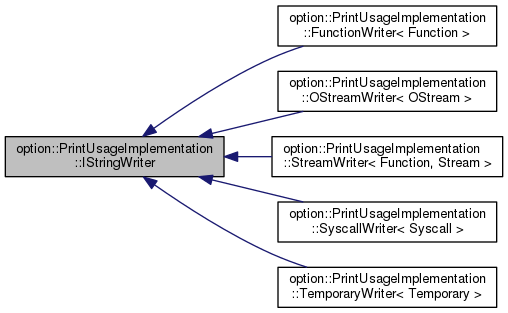
\includegraphics[width=350pt]{structoption_1_1PrintUsageImplementation_1_1IStringWriter__inherit__graph}
\end{center}
\end{figure}
\subsection*{Public Member Functions}
\begin{DoxyCompactItemize}
\item 
virtual void \hyperlink{structoption_1_1PrintUsageImplementation_1_1IStringWriter_a497172d92e09072a16996c127dd3def8}{operator()} (const char $\ast$, int)\hypertarget{structoption_1_1PrintUsageImplementation_1_1IStringWriter_a497172d92e09072a16996c127dd3def8}{}\label{structoption_1_1PrintUsageImplementation_1_1IStringWriter_a497172d92e09072a16996c127dd3def8}

\begin{DoxyCompactList}\small\item\em Writes the given number of chars beginning at the given pointer somewhere. \end{DoxyCompactList}\end{DoxyCompactItemize}


The documentation for this struct was generated from the following file\+:\begin{DoxyCompactItemize}
\item 
\hyperlink{optionparser_8h}{optionparser.\+h}\end{DoxyCompactItemize}

\hypertarget{classhebi_1_1Info_1_1LedField}{}\section{hebi\+:\+:Info\+:\+:Led\+Field Class Reference}
\label{classhebi_1_1Info_1_1LedField}\index{hebi\+::\+Info\+::\+Led\+Field@{hebi\+::\+Info\+::\+Led\+Field}}


A message field for interfacing with an L\+ED.  




{\ttfamily \#include $<$info.\+hpp$>$}

\subsection*{Public Member Functions}
\begin{DoxyCompactItemize}
\item 
\mbox{\Hypertarget{classhebi_1_1Info_1_1LedField_af012c0a7e7b4cbe1d41ad8a19441a157}\label{classhebi_1_1Info_1_1LedField_af012c0a7e7b4cbe1d41ad8a19441a157}} 
{\bfseries Led\+Field} (Hebi\+Info\+Ptr internal, Info\+Led\+Field field)
\item 
\hyperlink{classhebi_1_1Info_1_1LedField_ad01bb0b217fa57dd74e288cc70c0d59f}{operator bool} () const
\begin{DoxyCompactList}\small\item\em Allows casting to a bool to check if the L\+ED color is set without directly calling {\ttfamily \hyperlink{classhebi_1_1Info_1_1LedField_aa78e496273712fe789e5cc70b27831b4}{has\+Color()}}. \end{DoxyCompactList}\item 
\mbox{\Hypertarget{classhebi_1_1Info_1_1LedField_aa78e496273712fe789e5cc70b27831b4}\label{classhebi_1_1Info_1_1LedField_aa78e496273712fe789e5cc70b27831b4}} 
bool \hyperlink{classhebi_1_1Info_1_1LedField_aa78e496273712fe789e5cc70b27831b4}{has\+Color} () const
\begin{DoxyCompactList}\small\item\em Returns true if the L\+ED color is set, and false otherwise. \end{DoxyCompactList}\item 
\mbox{\Hypertarget{classhebi_1_1Info_1_1LedField_ad0e9274b9b4a4144303a04c7faf57c35}\label{classhebi_1_1Info_1_1LedField_ad0e9274b9b4a4144303a04c7faf57c35}} 
\hyperlink{structhebi_1_1Color}{Color} \hyperlink{classhebi_1_1Info_1_1LedField_ad0e9274b9b4a4144303a04c7faf57c35}{get\+Color} () const
\begin{DoxyCompactList}\small\item\em Returns the led color. \end{DoxyCompactList}\end{DoxyCompactItemize}


\subsection{Detailed Description}
A message field for interfacing with an L\+ED. 

\subsection{Member Function Documentation}
\mbox{\Hypertarget{classhebi_1_1Info_1_1LedField_ad01bb0b217fa57dd74e288cc70c0d59f}\label{classhebi_1_1Info_1_1LedField_ad01bb0b217fa57dd74e288cc70c0d59f}} 
\index{hebi\+::\+Info\+::\+Led\+Field@{hebi\+::\+Info\+::\+Led\+Field}!operator bool@{operator bool}}
\index{operator bool@{operator bool}!hebi\+::\+Info\+::\+Led\+Field@{hebi\+::\+Info\+::\+Led\+Field}}
\subsubsection{\texorpdfstring{operator bool()}{operator bool()}}
{\footnotesize\ttfamily hebi\+::\+Info\+::\+Led\+Field\+::operator bool (\begin{DoxyParamCaption}{ }\end{DoxyParamCaption}) const\hspace{0.3cm}{\ttfamily [inline]}, {\ttfamily [explicit]}}



Allows casting to a bool to check if the L\+ED color is set without directly calling {\ttfamily \hyperlink{classhebi_1_1Info_1_1LedField_aa78e496273712fe789e5cc70b27831b4}{has\+Color()}}. 

This can be used as in the following (assuming \textquotesingle{}parent\textquotesingle{} is a parent message, and this field is called \textquotesingle{}my\+Field\textquotesingle{}) 
\begin{DoxyCode}
Info::LedField& f = parent.myField();
\textcolor{keywordflow}{if} (f)
  std::cout << \textcolor{stringliteral}{"Field has color!"} << std::endl;
\textcolor{keywordflow}{else}
  std::cout << \textcolor{stringliteral}{"Field has no value!"} << std::endl;
\end{DoxyCode}
 

The documentation for this class was generated from the following files\+:\begin{DoxyCompactItemize}
\item 
info.\+hpp\item 
info.\+cpp\end{DoxyCompactItemize}

\hypertarget{classhebi_1_1Command_1_1LedField}{}\section{hebi\+:\+:Command\+:\+:Led\+Field Class Reference}
\label{classhebi_1_1Command_1_1LedField}\index{hebi\+::\+Command\+::\+Led\+Field@{hebi\+::\+Command\+::\+Led\+Field}}


A message field for interfacing with an L\+ED.  




{\ttfamily \#include $<$command.\+hpp$>$}

\subsection*{Public Member Functions}
\begin{DoxyCompactItemize}
\item 
{\bfseries Led\+Field} (Hebi\+Command\+Ptr internal, Command\+Led\+Field field)\hypertarget{classhebi_1_1Command_1_1LedField_a51c1a35f4ca0dc607f9627abebaaad5e}{}\label{classhebi_1_1Command_1_1LedField_a51c1a35f4ca0dc607f9627abebaaad5e}

\item 
bool \hyperlink{classhebi_1_1Command_1_1LedField_a28b30332afd8b31555f5fc75e4b1a44e}{has\+Color} () const \hypertarget{classhebi_1_1Command_1_1LedField_a28b30332afd8b31555f5fc75e4b1a44e}{}\label{classhebi_1_1Command_1_1LedField_a28b30332afd8b31555f5fc75e4b1a44e}

\begin{DoxyCompactList}\small\item\em Returns true if the L\+ED color is set, and false otherwise. \end{DoxyCompactList}\item 
bool \hyperlink{classhebi_1_1Command_1_1LedField_aae7b88394b6663c44e7cba94de51a7f3}{has\+Module\+Control} () const 
\begin{DoxyCompactList}\small\item\em Returns true if the message indicates that the module should resume control of the L\+ED. \end{DoxyCompactList}\item 
\hyperlink{structhebi_1_1Color}{Color} \hyperlink{classhebi_1_1Command_1_1LedField_a25c5054826a59ff3b314998d287e8feb}{get\+Color} () const \hypertarget{classhebi_1_1Command_1_1LedField_a25c5054826a59ff3b314998d287e8feb}{}\label{classhebi_1_1Command_1_1LedField_a25c5054826a59ff3b314998d287e8feb}

\begin{DoxyCompactList}\small\item\em Returns the led color. \end{DoxyCompactList}\item 
void \hyperlink{classhebi_1_1Command_1_1LedField_aa1c2fc432de51dba198988b5c285d6a4}{set\+Override\+Color} (const \hyperlink{structhebi_1_1Color}{Color} \&new\+\_\+color)\hypertarget{classhebi_1_1Command_1_1LedField_aa1c2fc432de51dba198988b5c285d6a4}{}\label{classhebi_1_1Command_1_1LedField_aa1c2fc432de51dba198988b5c285d6a4}

\begin{DoxyCompactList}\small\item\em Commands a color that overrides the module\textquotesingle{}s control of the L\+ED. \end{DoxyCompactList}\item 
void \hyperlink{classhebi_1_1Command_1_1LedField_a3f41b8c7cc1d1de4fe3d78683be62ef0}{set\+Module\+Control} ()\hypertarget{classhebi_1_1Command_1_1LedField_a3f41b8c7cc1d1de4fe3d78683be62ef0}{}\label{classhebi_1_1Command_1_1LedField_a3f41b8c7cc1d1de4fe3d78683be62ef0}

\begin{DoxyCompactList}\small\item\em Sets the module to regain control of the L\+ED. \end{DoxyCompactList}\item 
void \hyperlink{classhebi_1_1Command_1_1LedField_aa0e2f2c914e83e8b60ca9da40474dc15}{clear} ()\hypertarget{classhebi_1_1Command_1_1LedField_aa0e2f2c914e83e8b60ca9da40474dc15}{}\label{classhebi_1_1Command_1_1LedField_aa0e2f2c914e83e8b60ca9da40474dc15}

\begin{DoxyCompactList}\small\item\em Removes any currently set value for this field, so that the module maintains its previous state of L\+ED control/color (i.\+e., does not have an override color command or an explicit \textquotesingle{}module control\textquotesingle{} command). \end{DoxyCompactList}\end{DoxyCompactItemize}


\subsection{Detailed Description}
A message field for interfacing with an L\+ED. 

\subsection{Member Function Documentation}
\index{hebi\+::\+Command\+::\+Led\+Field@{hebi\+::\+Command\+::\+Led\+Field}!has\+Module\+Control@{has\+Module\+Control}}
\index{has\+Module\+Control@{has\+Module\+Control}!hebi\+::\+Command\+::\+Led\+Field@{hebi\+::\+Command\+::\+Led\+Field}}
\subsubsection[{\texorpdfstring{has\+Module\+Control() const }{hasModuleControl() const }}]{\setlength{\rightskip}{0pt plus 5cm}bool hebi\+::\+Command\+::\+Led\+Field\+::has\+Module\+Control (
\begin{DoxyParamCaption}
{}
\end{DoxyParamCaption}
) const}\hypertarget{classhebi_1_1Command_1_1LedField_aae7b88394b6663c44e7cba94de51a7f3}{}\label{classhebi_1_1Command_1_1LedField_aae7b88394b6663c44e7cba94de51a7f3}


Returns true if the message indicates that the module should resume control of the L\+ED. 

Note\+: a return value of {\ttfamily false} can indicate either an override command (if and only if {\ttfamily \hyperlink{classhebi_1_1Command_1_1LedField_a28b30332afd8b31555f5fc75e4b1a44e}{has\+Color()}} returns {\ttfamily true}), or no information about the L\+ED (i.\+e., the module should maintain it\textquotesingle{}s current state regarding the L\+ED). 

The documentation for this class was generated from the following files\+:\begin{DoxyCompactItemize}
\item 
command.\+hpp\item 
command.\+cpp\end{DoxyCompactItemize}

\hypertarget{classhebi_1_1Feedback_1_1LedField}{}\section{hebi\+:\+:Feedback\+:\+:Led\+Field Class Reference}
\label{classhebi_1_1Feedback_1_1LedField}\index{hebi\+::\+Feedback\+::\+Led\+Field@{hebi\+::\+Feedback\+::\+Led\+Field}}


A message field for interfacing with an L\+ED.  




{\ttfamily \#include $<$feedback.\+hpp$>$}

\subsection*{Public Member Functions}
\begin{DoxyCompactItemize}
\item 
{\bfseries Led\+Field} (Hebi\+Feedback\+Ptr internal, Feedback\+Led\+Field field)\hypertarget{classhebi_1_1Feedback_1_1LedField_a3bb6871c57c7eb4b00d15ad001ec1fb0}{}\label{classhebi_1_1Feedback_1_1LedField_a3bb6871c57c7eb4b00d15ad001ec1fb0}

\item 
\hyperlink{classhebi_1_1Feedback_1_1LedField_a725454852c3c9f1e71022f7e51ecf6e6}{operator bool} () const 
\begin{DoxyCompactList}\small\item\em Allows casting to a bool to check if the L\+ED color is set without directly calling {\ttfamily \hyperlink{classhebi_1_1Feedback_1_1LedField_a9fb5bd115347991e476e89c7da783f78}{has\+Color()}}. \end{DoxyCompactList}\item 
bool \hyperlink{classhebi_1_1Feedback_1_1LedField_a9fb5bd115347991e476e89c7da783f78}{has\+Color} () const \hypertarget{classhebi_1_1Feedback_1_1LedField_a9fb5bd115347991e476e89c7da783f78}{}\label{classhebi_1_1Feedback_1_1LedField_a9fb5bd115347991e476e89c7da783f78}

\begin{DoxyCompactList}\small\item\em Returns true if the L\+ED color is set, and false otherwise. \end{DoxyCompactList}\item 
\hyperlink{structhebi_1_1Color}{Color} \hyperlink{classhebi_1_1Feedback_1_1LedField_a0040ce588480d51787ddce6f51c15326}{get\+Color} () const \hypertarget{classhebi_1_1Feedback_1_1LedField_a0040ce588480d51787ddce6f51c15326}{}\label{classhebi_1_1Feedback_1_1LedField_a0040ce588480d51787ddce6f51c15326}

\begin{DoxyCompactList}\small\item\em Returns the led color. \end{DoxyCompactList}\end{DoxyCompactItemize}


\subsection{Detailed Description}
A message field for interfacing with an L\+ED. 

\subsection{Member Function Documentation}
\index{hebi\+::\+Feedback\+::\+Led\+Field@{hebi\+::\+Feedback\+::\+Led\+Field}!operator bool@{operator bool}}
\index{operator bool@{operator bool}!hebi\+::\+Feedback\+::\+Led\+Field@{hebi\+::\+Feedback\+::\+Led\+Field}}
\subsubsection[{\texorpdfstring{operator bool() const }{operator bool() const }}]{\setlength{\rightskip}{0pt plus 5cm}hebi\+::\+Feedback\+::\+Led\+Field\+::operator bool (
\begin{DoxyParamCaption}
{}
\end{DoxyParamCaption}
) const\hspace{0.3cm}{\ttfamily [inline]}, {\ttfamily [explicit]}}\hypertarget{classhebi_1_1Feedback_1_1LedField_a725454852c3c9f1e71022f7e51ecf6e6}{}\label{classhebi_1_1Feedback_1_1LedField_a725454852c3c9f1e71022f7e51ecf6e6}


Allows casting to a bool to check if the L\+ED color is set without directly calling {\ttfamily \hyperlink{classhebi_1_1Feedback_1_1LedField_a9fb5bd115347991e476e89c7da783f78}{has\+Color()}}. 

This can be used as in the following (assuming \textquotesingle{}parent\textquotesingle{} is a parent message, and this field is called \textquotesingle{}my\+Field\textquotesingle{}) 
\begin{DoxyCode}
Feedback::LedField& f = parent.myField();
\textcolor{keywordflow}{if} (f)
  std::cout << \textcolor{stringliteral}{"Field has color!"} << std::endl;
\textcolor{keywordflow}{else}
  std::cout << \textcolor{stringliteral}{"Field has no value!"} << std::endl;
\end{DoxyCode}
 

The documentation for this class was generated from the following files\+:\begin{DoxyCompactItemize}
\item 
feedback.\+hpp\item 
feedback.\+cpp\end{DoxyCompactItemize}

\hypertarget{classoption_1_1PrintUsageImplementation_1_1LinePartIterator}{}\section{option\+:\+:Print\+Usage\+Implementation\+:\+:Line\+Part\+Iterator Class Reference}
\label{classoption_1_1PrintUsageImplementation_1_1LinePartIterator}\index{option\+::\+Print\+Usage\+Implementation\+::\+Line\+Part\+Iterator@{option\+::\+Print\+Usage\+Implementation\+::\+Line\+Part\+Iterator}}
\subsection*{Public Member Functions}
\begin{DoxyCompactItemize}
\item 
\hyperlink{classoption_1_1PrintUsageImplementation_1_1LinePartIterator_a8a61fef9ba907fd4e10ff0fd772ee5e7}{Line\+Part\+Iterator} (const \hyperlink{structoption_1_1Descriptor}{Descriptor} usage\mbox{[}$\,$\mbox{]})\hypertarget{classoption_1_1PrintUsageImplementation_1_1LinePartIterator_a8a61fef9ba907fd4e10ff0fd772ee5e7}{}\label{classoption_1_1PrintUsageImplementation_1_1LinePartIterator_a8a61fef9ba907fd4e10ff0fd772ee5e7}

\begin{DoxyCompactList}\small\item\em Creates an iterator for {\ttfamily usage}. \end{DoxyCompactList}\item 
bool \hyperlink{classoption_1_1PrintUsageImplementation_1_1LinePartIterator_afe43ca12d399ed3c871e4dc5bf63356e}{next\+Table} ()
\begin{DoxyCompactList}\small\item\em Moves iteration to the next table (if any). Has to be called once on a new \hyperlink{classoption_1_1PrintUsageImplementation_1_1LinePartIterator}{Line\+Part\+Iterator} to move to the 1st table. \end{DoxyCompactList}\item 
void \hyperlink{classoption_1_1PrintUsageImplementation_1_1LinePartIterator_a0cbe8ed79ab4958a70b957598dd76fa6}{restart\+Table} ()\hypertarget{classoption_1_1PrintUsageImplementation_1_1LinePartIterator_a0cbe8ed79ab4958a70b957598dd76fa6}{}\label{classoption_1_1PrintUsageImplementation_1_1LinePartIterator_a0cbe8ed79ab4958a70b957598dd76fa6}

\begin{DoxyCompactList}\small\item\em Reset iteration to the beginning of the current table. \end{DoxyCompactList}\item 
bool \hyperlink{classoption_1_1PrintUsageImplementation_1_1LinePartIterator_a55d5c3e50f9c1d8cd48f518899a5a48c}{next\+Row} ()
\begin{DoxyCompactList}\small\item\em Moves iteration to the next row (if any). Has to be called once after each call to \hyperlink{classoption_1_1PrintUsageImplementation_1_1LinePartIterator_afe43ca12d399ed3c871e4dc5bf63356e}{next\+Table()} to move to the 1st row of the table. \end{DoxyCompactList}\item 
void \hyperlink{classoption_1_1PrintUsageImplementation_1_1LinePartIterator_a96c448939f33a811174ea7b5addb312e}{restart\+Row} ()\hypertarget{classoption_1_1PrintUsageImplementation_1_1LinePartIterator_a96c448939f33a811174ea7b5addb312e}{}\label{classoption_1_1PrintUsageImplementation_1_1LinePartIterator_a96c448939f33a811174ea7b5addb312e}

\begin{DoxyCompactList}\small\item\em Reset iteration to the beginning of the current row. \end{DoxyCompactList}\item 
bool \hyperlink{classoption_1_1PrintUsageImplementation_1_1LinePartIterator_a58b8743da57de2d108472eee60324df6}{next} ()
\begin{DoxyCompactList}\small\item\em Moves iteration to the next part (if any). Has to be called once after each call to \hyperlink{classoption_1_1PrintUsageImplementation_1_1LinePartIterator_a55d5c3e50f9c1d8cd48f518899a5a48c}{next\+Row()} to move to the 1st part of the row. \end{DoxyCompactList}\item 
int \hyperlink{classoption_1_1PrintUsageImplementation_1_1LinePartIterator_afa41382acabcd37ca70f7e8b9994b8c0}{column} ()\hypertarget{classoption_1_1PrintUsageImplementation_1_1LinePartIterator_afa41382acabcd37ca70f7e8b9994b8c0}{}\label{classoption_1_1PrintUsageImplementation_1_1LinePartIterator_afa41382acabcd37ca70f7e8b9994b8c0}

\begin{DoxyCompactList}\small\item\em Returns the index (counting from 0) of the column in which the part pointed to by \hyperlink{classoption_1_1PrintUsageImplementation_1_1LinePartIterator_ada26229add63bd479c7877f2f8e32908}{data()} is located. \end{DoxyCompactList}\item 
int \hyperlink{classoption_1_1PrintUsageImplementation_1_1LinePartIterator_a8ad1201d95bf0bd9453a731da8c15a10}{line} ()\hypertarget{classoption_1_1PrintUsageImplementation_1_1LinePartIterator_a8ad1201d95bf0bd9453a731da8c15a10}{}\label{classoption_1_1PrintUsageImplementation_1_1LinePartIterator_a8ad1201d95bf0bd9453a731da8c15a10}

\begin{DoxyCompactList}\small\item\em Returns the index (counting from 0) of the line within the current column this part belongs to. \end{DoxyCompactList}\item 
int \hyperlink{classoption_1_1PrintUsageImplementation_1_1LinePartIterator_a557e521cb41e951a34df2737d25f9dce}{length} ()\hypertarget{classoption_1_1PrintUsageImplementation_1_1LinePartIterator_a557e521cb41e951a34df2737d25f9dce}{}\label{classoption_1_1PrintUsageImplementation_1_1LinePartIterator_a557e521cb41e951a34df2737d25f9dce}

\begin{DoxyCompactList}\small\item\em Returns the length of the part pointed to by \hyperlink{classoption_1_1PrintUsageImplementation_1_1LinePartIterator_ada26229add63bd479c7877f2f8e32908}{data()} in raw chars (not U\+T\+F-\/8 characters). \end{DoxyCompactList}\item 
int \hyperlink{classoption_1_1PrintUsageImplementation_1_1LinePartIterator_a03b6fedfe805d7fc73216da5cd33270e}{screen\+Length} ()\hypertarget{classoption_1_1PrintUsageImplementation_1_1LinePartIterator_a03b6fedfe805d7fc73216da5cd33270e}{}\label{classoption_1_1PrintUsageImplementation_1_1LinePartIterator_a03b6fedfe805d7fc73216da5cd33270e}

\begin{DoxyCompactList}\small\item\em Returns the width in screen columns of the part pointed to by \hyperlink{classoption_1_1PrintUsageImplementation_1_1LinePartIterator_ada26229add63bd479c7877f2f8e32908}{data()}. Takes multi-\/byte U\+T\+F-\/8 sequences and wide characters into account. \end{DoxyCompactList}\item 
const char $\ast$ \hyperlink{classoption_1_1PrintUsageImplementation_1_1LinePartIterator_ada26229add63bd479c7877f2f8e32908}{data} ()\hypertarget{classoption_1_1PrintUsageImplementation_1_1LinePartIterator_ada26229add63bd479c7877f2f8e32908}{}\label{classoption_1_1PrintUsageImplementation_1_1LinePartIterator_ada26229add63bd479c7877f2f8e32908}

\begin{DoxyCompactList}\small\item\em Returns the current part of the iteration. \end{DoxyCompactList}\end{DoxyCompactItemize}


\subsection{Member Function Documentation}
\index{option\+::\+Print\+Usage\+Implementation\+::\+Line\+Part\+Iterator@{option\+::\+Print\+Usage\+Implementation\+::\+Line\+Part\+Iterator}!next@{next}}
\index{next@{next}!option\+::\+Print\+Usage\+Implementation\+::\+Line\+Part\+Iterator@{option\+::\+Print\+Usage\+Implementation\+::\+Line\+Part\+Iterator}}
\subsubsection[{\texorpdfstring{next()}{next()}}]{\setlength{\rightskip}{0pt plus 5cm}bool option\+::\+Print\+Usage\+Implementation\+::\+Line\+Part\+Iterator\+::next (
\begin{DoxyParamCaption}
{}
\end{DoxyParamCaption}
)\hspace{0.3cm}{\ttfamily [inline]}}\hypertarget{classoption_1_1PrintUsageImplementation_1_1LinePartIterator_a58b8743da57de2d108472eee60324df6}{}\label{classoption_1_1PrintUsageImplementation_1_1LinePartIterator_a58b8743da57de2d108472eee60324df6}


Moves iteration to the next part (if any). Has to be called once after each call to \hyperlink{classoption_1_1PrintUsageImplementation_1_1LinePartIterator_a55d5c3e50f9c1d8cd48f518899a5a48c}{next\+Row()} to move to the 1st part of the row. 


\begin{DoxyRetVals}{Return values}
{\em false} & if moving to next part failed because no further part exists.\\
\hline
\end{DoxyRetVals}
See \hyperlink{classoption_1_1PrintUsageImplementation_1_1LinePartIterator}{Line\+Part\+Iterator} for details about the iteration. \index{option\+::\+Print\+Usage\+Implementation\+::\+Line\+Part\+Iterator@{option\+::\+Print\+Usage\+Implementation\+::\+Line\+Part\+Iterator}!next\+Row@{next\+Row}}
\index{next\+Row@{next\+Row}!option\+::\+Print\+Usage\+Implementation\+::\+Line\+Part\+Iterator@{option\+::\+Print\+Usage\+Implementation\+::\+Line\+Part\+Iterator}}
\subsubsection[{\texorpdfstring{next\+Row()}{nextRow()}}]{\setlength{\rightskip}{0pt plus 5cm}bool option\+::\+Print\+Usage\+Implementation\+::\+Line\+Part\+Iterator\+::next\+Row (
\begin{DoxyParamCaption}
{}
\end{DoxyParamCaption}
)\hspace{0.3cm}{\ttfamily [inline]}}\hypertarget{classoption_1_1PrintUsageImplementation_1_1LinePartIterator_a55d5c3e50f9c1d8cd48f518899a5a48c}{}\label{classoption_1_1PrintUsageImplementation_1_1LinePartIterator_a55d5c3e50f9c1d8cd48f518899a5a48c}


Moves iteration to the next row (if any). Has to be called once after each call to \hyperlink{classoption_1_1PrintUsageImplementation_1_1LinePartIterator_afe43ca12d399ed3c871e4dc5bf63356e}{next\+Table()} to move to the 1st row of the table. 


\begin{DoxyRetVals}{Return values}
{\em false} & if moving to next row failed because no further row exists. \\
\hline
\end{DoxyRetVals}
\index{option\+::\+Print\+Usage\+Implementation\+::\+Line\+Part\+Iterator@{option\+::\+Print\+Usage\+Implementation\+::\+Line\+Part\+Iterator}!next\+Table@{next\+Table}}
\index{next\+Table@{next\+Table}!option\+::\+Print\+Usage\+Implementation\+::\+Line\+Part\+Iterator@{option\+::\+Print\+Usage\+Implementation\+::\+Line\+Part\+Iterator}}
\subsubsection[{\texorpdfstring{next\+Table()}{nextTable()}}]{\setlength{\rightskip}{0pt plus 5cm}bool option\+::\+Print\+Usage\+Implementation\+::\+Line\+Part\+Iterator\+::next\+Table (
\begin{DoxyParamCaption}
{}
\end{DoxyParamCaption}
)\hspace{0.3cm}{\ttfamily [inline]}}\hypertarget{classoption_1_1PrintUsageImplementation_1_1LinePartIterator_afe43ca12d399ed3c871e4dc5bf63356e}{}\label{classoption_1_1PrintUsageImplementation_1_1LinePartIterator_afe43ca12d399ed3c871e4dc5bf63356e}


Moves iteration to the next table (if any). Has to be called once on a new \hyperlink{classoption_1_1PrintUsageImplementation_1_1LinePartIterator}{Line\+Part\+Iterator} to move to the 1st table. 


\begin{DoxyRetVals}{Return values}
{\em false} & if moving to next table failed because no further table exists. \\
\hline
\end{DoxyRetVals}


The documentation for this class was generated from the following file\+:\begin{DoxyCompactItemize}
\item 
\hyperlink{optionparser_8h}{optionparser.\+h}\end{DoxyCompactItemize}

\hypertarget{classoption_1_1PrintUsageImplementation_1_1LineWrapper}{}\section{option\+:\+:Print\+Usage\+Implementation\+:\+:Line\+Wrapper Class Reference}
\label{classoption_1_1PrintUsageImplementation_1_1LineWrapper}\index{option\+::\+Print\+Usage\+Implementation\+::\+Line\+Wrapper@{option\+::\+Print\+Usage\+Implementation\+::\+Line\+Wrapper}}
\subsection*{Public Member Functions}
\begin{DoxyCompactItemize}
\item 
\mbox{\Hypertarget{classoption_1_1PrintUsageImplementation_1_1LineWrapper_a9383db9fd3fb18ce091db63ce0b149fd}\label{classoption_1_1PrintUsageImplementation_1_1LineWrapper_a9383db9fd3fb18ce091db63ce0b149fd}} 
void \hyperlink{classoption_1_1PrintUsageImplementation_1_1LineWrapper_a9383db9fd3fb18ce091db63ce0b149fd}{flush} (\hyperlink{structoption_1_1PrintUsageImplementation_1_1IStringWriter}{I\+String\+Writer} \&write)
\begin{DoxyCompactList}\small\item\em Writes out all remaining data from the \hyperlink{classoption_1_1PrintUsageImplementation_1_1LineWrapper}{Line\+Wrapper} using {\ttfamily write}. Unlike \hyperlink{classoption_1_1PrintUsageImplementation_1_1LineWrapper_add20eca40865ad892d6c28b412ac14d5}{process()} this method indents all lines including the first and will output a \textbackslash{}n at the end (but only if something has been written). \end{DoxyCompactList}\item 
void \hyperlink{classoption_1_1PrintUsageImplementation_1_1LineWrapper_add20eca40865ad892d6c28b412ac14d5}{process} (\hyperlink{structoption_1_1PrintUsageImplementation_1_1IStringWriter}{I\+String\+Writer} \&write, const char $\ast$data, int len)
\begin{DoxyCompactList}\small\item\em Process, wrap and output the next piece of data. \end{DoxyCompactList}\item 
\hyperlink{classoption_1_1PrintUsageImplementation_1_1LineWrapper_a288f16b6e928e9f54f48e13ff6817e95}{Line\+Wrapper} (int x1, int x2)
\begin{DoxyCompactList}\small\item\em Constructs a \hyperlink{classoption_1_1PrintUsageImplementation_1_1LineWrapper}{Line\+Wrapper} that wraps its output to fit into screen columns {\ttfamily x1} (incl.) to {\ttfamily x2} (excl.). \end{DoxyCompactList}\end{DoxyCompactItemize}


\subsection{Constructor \& Destructor Documentation}
\mbox{\Hypertarget{classoption_1_1PrintUsageImplementation_1_1LineWrapper_a288f16b6e928e9f54f48e13ff6817e95}\label{classoption_1_1PrintUsageImplementation_1_1LineWrapper_a288f16b6e928e9f54f48e13ff6817e95}} 
\index{option\+::\+Print\+Usage\+Implementation\+::\+Line\+Wrapper@{option\+::\+Print\+Usage\+Implementation\+::\+Line\+Wrapper}!Line\+Wrapper@{Line\+Wrapper}}
\index{Line\+Wrapper@{Line\+Wrapper}!option\+::\+Print\+Usage\+Implementation\+::\+Line\+Wrapper@{option\+::\+Print\+Usage\+Implementation\+::\+Line\+Wrapper}}
\subsubsection{\texorpdfstring{Line\+Wrapper()}{LineWrapper()}}
{\footnotesize\ttfamily option\+::\+Print\+Usage\+Implementation\+::\+Line\+Wrapper\+::\+Line\+Wrapper (\begin{DoxyParamCaption}\item[{int}]{x1,  }\item[{int}]{x2 }\end{DoxyParamCaption})\hspace{0.3cm}{\ttfamily [inline]}}



Constructs a \hyperlink{classoption_1_1PrintUsageImplementation_1_1LineWrapper}{Line\+Wrapper} that wraps its output to fit into screen columns {\ttfamily x1} (incl.) to {\ttfamily x2} (excl.). 

{\ttfamily x1} gives the indentation \hyperlink{classoption_1_1PrintUsageImplementation_1_1LineWrapper}{Line\+Wrapper} uses if it needs to indent. 

\subsection{Member Function Documentation}
\mbox{\Hypertarget{classoption_1_1PrintUsageImplementation_1_1LineWrapper_add20eca40865ad892d6c28b412ac14d5}\label{classoption_1_1PrintUsageImplementation_1_1LineWrapper_add20eca40865ad892d6c28b412ac14d5}} 
\index{option\+::\+Print\+Usage\+Implementation\+::\+Line\+Wrapper@{option\+::\+Print\+Usage\+Implementation\+::\+Line\+Wrapper}!process@{process}}
\index{process@{process}!option\+::\+Print\+Usage\+Implementation\+::\+Line\+Wrapper@{option\+::\+Print\+Usage\+Implementation\+::\+Line\+Wrapper}}
\subsubsection{\texorpdfstring{process()}{process()}}
{\footnotesize\ttfamily void option\+::\+Print\+Usage\+Implementation\+::\+Line\+Wrapper\+::process (\begin{DoxyParamCaption}\item[{\hyperlink{structoption_1_1PrintUsageImplementation_1_1IStringWriter}{I\+String\+Writer} \&}]{write,  }\item[{const char $\ast$}]{data,  }\item[{int}]{len }\end{DoxyParamCaption})\hspace{0.3cm}{\ttfamily [inline]}}



Process, wrap and output the next piece of data. 

\hyperlink{classoption_1_1PrintUsageImplementation_1_1LineWrapper_add20eca40865ad892d6c28b412ac14d5}{process()} will output at least one line of output. This is not necessarily the {\ttfamily data} passed in. It may be data queued from a prior call to \hyperlink{classoption_1_1PrintUsageImplementation_1_1LineWrapper_add20eca40865ad892d6c28b412ac14d5}{process()}. If the internal buffer is full, more than 1 line will be output.

\hyperlink{classoption_1_1PrintUsageImplementation_1_1LineWrapper_add20eca40865ad892d6c28b412ac14d5}{process()} assumes that the a proper amount of indentation has already been output. It won\textquotesingle{}t write any further indentation before the 1st line. If more than 1 line is written due to buffer constraints, the lines following the first will be indented by this method, though.

No \textbackslash{}n is written by this method after the last line that is written.


\begin{DoxyParams}{Parameters}
{\em write} & where to write the data. \\
\hline
{\em data} & the new chunk of data to write. \\
\hline
{\em len} & the length of the chunk of data to write. \\
\hline
\end{DoxyParams}


The documentation for this class was generated from the following file\+:\begin{DoxyCompactItemize}
\item 
\hyperlink{optionparser_8h}{optionparser.\+h}\end{DoxyCompactItemize}

\hypertarget{classhebi_1_1Lookup}{}\section{hebi\+:\+:Lookup Class Reference}
\label{classhebi_1_1Lookup}\index{hebi\+::\+Lookup@{hebi\+::\+Lookup}}


Maintains a registry of network-\/connected modules and returns \hyperlink{classhebi_1_1Module}{Module} and \hyperlink{classhebi_1_1Group}{Group} objects to the user.  




{\ttfamily \#include $<$lookup.\+hpp$>$}

\subsection*{Public Member Functions}
\begin{DoxyCompactItemize}
\item 
\hyperlink{classhebi_1_1Lookup_acdfa87d652dd197ff578e5ea0f25128c}{Lookup} ()
\begin{DoxyCompactList}\small\item\em Creates a \hyperlink{classhebi_1_1Lookup}{Lookup} object which can create \hyperlink{classhebi_1_1Module}{Module} and \hyperlink{classhebi_1_1Group}{Group} references. Typically, only one \hyperlink{classhebi_1_1Lookup}{Lookup} object should exist at a time. \end{DoxyCompactList}\item 
\mbox{\Hypertarget{classhebi_1_1Lookup_a7d9e38f258c85bedfd63c71c41d1bd8b}\label{classhebi_1_1Lookup_a7d9e38f258c85bedfd63c71c41d1bd8b}} 
virtual \hyperlink{classhebi_1_1Lookup_a7d9e38f258c85bedfd63c71c41d1bd8b}{$\sim$\+Lookup} () noexcept
\begin{DoxyCompactList}\small\item\em Destructor frees all resources created by \hyperlink{classhebi_1_1Lookup}{Lookup} object, and stops the background query thread. \end{DoxyCompactList}\item 
void \hyperlink{classhebi_1_1Lookup_a52e3d10c45ac8b6c47a7944fee1d7189}{print\+Table} ()
\begin{DoxyCompactList}\small\item\em Displays the current contents of the module registry on stdout -- i.\+e., which modules have been found by the lookup. \end{DoxyCompactList}\item 
std\+::unique\+\_\+ptr$<$ \hyperlink{classhebi_1_1Module}{Module} $>$ \hyperlink{classhebi_1_1Lookup_aaee883fe7e060f0ea0638a09bc49f54b}{get\+Module\+From\+Name} (const std\+::string \&name, const std\+::string \&family, long timeout\+\_\+ms=D\+E\+F\+A\+U\+L\+T\+\_\+\+T\+I\+M\+E\+O\+UT)
\begin{DoxyCompactList}\small\item\em Get a module with the given name and family. \end{DoxyCompactList}\item 
std\+::unique\+\_\+ptr$<$ \hyperlink{classhebi_1_1Module}{Module} $>$ \hyperlink{classhebi_1_1Lookup_ad4078193d720554b57bfd47a46d35231}{get\+Module\+From\+Mac} (const \hyperlink{classhebi_1_1MacAddress}{Mac\+Address} \&address, long timeout\+\_\+ms=D\+E\+F\+A\+U\+L\+T\+\_\+\+T\+I\+M\+E\+O\+UT)
\begin{DoxyCompactList}\small\item\em Get a module with the given mac address. \end{DoxyCompactList}\item 
std\+::unique\+\_\+ptr$<$ \hyperlink{classhebi_1_1Group}{Group} $>$ \hyperlink{classhebi_1_1Lookup_adae9314e23d17ad53e26f146f4c256bf}{get\+Group\+From\+Names} (const std\+::vector$<$ std\+::string $>$ \&names, const std\+::vector$<$ std\+::string $>$ \&families, long timeout\+\_\+ms=D\+E\+F\+A\+U\+L\+T\+\_\+\+T\+I\+M\+E\+O\+UT)
\begin{DoxyCompactList}\small\item\em Get a group from modules with the given names and families. \end{DoxyCompactList}\item 
std\+::unique\+\_\+ptr$<$ \hyperlink{classhebi_1_1Group}{Group} $>$ \hyperlink{classhebi_1_1Lookup_aad6bf0015b82dbce0b4dde06e1b10f52}{get\+Group\+From\+Macs} (const std\+::vector$<$ \hyperlink{classhebi_1_1MacAddress}{Mac\+Address} $>$ \&addresses, long timeout\+\_\+ms=D\+E\+F\+A\+U\+L\+T\+\_\+\+T\+I\+M\+E\+O\+UT)
\begin{DoxyCompactList}\small\item\em Get a group from modules with the given mac addresses. \end{DoxyCompactList}\item 
std\+::unique\+\_\+ptr$<$ \hyperlink{classhebi_1_1Group}{Group} $>$ \hyperlink{classhebi_1_1Lookup_a61243d9e23909ecc5511258452d4396f}{get\+Group\+From\+Family} (const std\+::string \&family, long timeout\+\_\+ms=D\+E\+F\+A\+U\+L\+T\+\_\+\+T\+I\+M\+E\+O\+UT)
\begin{DoxyCompactList}\small\item\em Get a group from all known modules with the given family. \end{DoxyCompactList}\item 
std\+::unique\+\_\+ptr$<$ \hyperlink{classhebi_1_1Group}{Group} $>$ \hyperlink{classhebi_1_1Lookup_afb22de42b4310292bd9a0a5848e3f3e6}{get\+Connected\+Group\+From\+Name} (const std\+::string \&name, const std\+::string \&family, long timeout\+\_\+ms=D\+E\+F\+A\+U\+L\+T\+\_\+\+T\+I\+M\+E\+O\+UT)
\begin{DoxyCompactList}\small\item\em Get a group from all modules known to connect to a module with the given name and family. \end{DoxyCompactList}\item 
std\+::unique\+\_\+ptr$<$ \hyperlink{classhebi_1_1Group}{Group} $>$ \hyperlink{classhebi_1_1Lookup_ad77bc157e336ee526157d5b31eb6bc22}{get\+Connected\+Group\+From\+Mac} (const \hyperlink{classhebi_1_1MacAddress}{Mac\+Address} \&address, long timeout\+\_\+ms=D\+E\+F\+A\+U\+L\+T\+\_\+\+T\+I\+M\+E\+O\+UT)
\begin{DoxyCompactList}\small\item\em Get a group from all modules known to connect to a module with the given mac address. \end{DoxyCompactList}\end{DoxyCompactItemize}


\subsection{Detailed Description}
Maintains a registry of network-\/connected modules and returns \hyperlink{classhebi_1_1Module}{Module} and \hyperlink{classhebi_1_1Group}{Group} objects to the user. 

Only one \hyperlink{classhebi_1_1Lookup}{Lookup} object is needed per application.

\begin{DoxyAuthor}{Author}
Matthew Tesch $<$ matt @ hebirobotics.\+com $>$ 
\end{DoxyAuthor}
\begin{DoxySince}{Since}
18 Feb 2016 
\end{DoxySince}


\subsection{Constructor \& Destructor Documentation}
\mbox{\Hypertarget{classhebi_1_1Lookup_acdfa87d652dd197ff578e5ea0f25128c}\label{classhebi_1_1Lookup_acdfa87d652dd197ff578e5ea0f25128c}} 
\index{hebi\+::\+Lookup@{hebi\+::\+Lookup}!Lookup@{Lookup}}
\index{Lookup@{Lookup}!hebi\+::\+Lookup@{hebi\+::\+Lookup}}
\subsubsection{\texorpdfstring{Lookup()}{Lookup()}}
{\footnotesize\ttfamily hebi\+::\+Lookup\+::\+Lookup (\begin{DoxyParamCaption}{ }\end{DoxyParamCaption})}



Creates a \hyperlink{classhebi_1_1Lookup}{Lookup} object which can create \hyperlink{classhebi_1_1Module}{Module} and \hyperlink{classhebi_1_1Group}{Group} references. Typically, only one \hyperlink{classhebi_1_1Lookup}{Lookup} object should exist at a time. 

Note that this call invokes a background thread to query the network for modules at regular intervals. 

\subsection{Member Function Documentation}
\mbox{\Hypertarget{classhebi_1_1Lookup_ad77bc157e336ee526157d5b31eb6bc22}\label{classhebi_1_1Lookup_ad77bc157e336ee526157d5b31eb6bc22}} 
\index{hebi\+::\+Lookup@{hebi\+::\+Lookup}!get\+Connected\+Group\+From\+Mac@{get\+Connected\+Group\+From\+Mac}}
\index{get\+Connected\+Group\+From\+Mac@{get\+Connected\+Group\+From\+Mac}!hebi\+::\+Lookup@{hebi\+::\+Lookup}}
\subsubsection{\texorpdfstring{get\+Connected\+Group\+From\+Mac()}{getConnectedGroupFromMac()}}
{\footnotesize\ttfamily std\+::unique\+\_\+ptr$<$ \hyperlink{classhebi_1_1Group}{Group} $>$ hebi\+::\+Lookup\+::get\+Connected\+Group\+From\+Mac (\begin{DoxyParamCaption}\item[{const \hyperlink{classhebi_1_1MacAddress}{Mac\+Address} \&}]{address,  }\item[{long}]{timeout\+\_\+ms = {\ttfamily DEFAULT\+\_\+TIMEOUT} }\end{DoxyParamCaption})}



Get a group from all modules known to connect to a module with the given mac address. 

Blocking call which returns a reference to a \hyperlink{classhebi_1_1Group}{Group} object with the given parameters. Times out after timeout\+\_\+msec milliseconds.


\begin{DoxyParams}{Parameters}
{\em address} & Physical mac address of the module to form the group from. \\
\hline
{\em timeout\+\_\+ms} & Timeout in milliseconds. A value of -\/1 blocks until a group is found, and a value of 0 returns immediately if no group with that address is currently known by the \hyperlink{classhebi_1_1Lookup}{Lookup} class. \\
\hline
\end{DoxyParams}
\begin{DoxyReturn}{Returns}
A unique\+\_\+ptr with no reference if no group found in allotted time, or reference to a newly allocated group object corresponding to the given parameters otherwise. 
\end{DoxyReturn}
\mbox{\Hypertarget{classhebi_1_1Lookup_afb22de42b4310292bd9a0a5848e3f3e6}\label{classhebi_1_1Lookup_afb22de42b4310292bd9a0a5848e3f3e6}} 
\index{hebi\+::\+Lookup@{hebi\+::\+Lookup}!get\+Connected\+Group\+From\+Name@{get\+Connected\+Group\+From\+Name}}
\index{get\+Connected\+Group\+From\+Name@{get\+Connected\+Group\+From\+Name}!hebi\+::\+Lookup@{hebi\+::\+Lookup}}
\subsubsection{\texorpdfstring{get\+Connected\+Group\+From\+Name()}{getConnectedGroupFromName()}}
{\footnotesize\ttfamily std\+::unique\+\_\+ptr$<$ \hyperlink{classhebi_1_1Group}{Group} $>$ hebi\+::\+Lookup\+::get\+Connected\+Group\+From\+Name (\begin{DoxyParamCaption}\item[{const std\+::string \&}]{name,  }\item[{const std\+::string \&}]{family,  }\item[{long}]{timeout\+\_\+ms = {\ttfamily DEFAULT\+\_\+TIMEOUT} }\end{DoxyParamCaption})}



Get a group from all modules known to connect to a module with the given name and family. 

Blocking call which returns a reference to a \hyperlink{classhebi_1_1Group}{Group} object with the given parameters. Times out after timeout\+\_\+msec milliseconds.


\begin{DoxyParams}{Parameters}
{\em name} & The given name of the module, as viewable in the H\+E\+BI G\+UI, to form the group from. \\
\hline
{\em family} & The given family of the module, as viewable in the H\+E\+BI G\+UI, to form the group from. \\
\hline
{\em timeout\+\_\+ms} & Timeout in milliseconds. A value of -\/1 blocks until a group is found, and a value of 0 returns immediately if no group with that address is currently known by the \hyperlink{classhebi_1_1Lookup}{Lookup} class. \\
\hline
\end{DoxyParams}
\begin{DoxyReturn}{Returns}
A unique\+\_\+ptr with no reference if no group found in allotted time, or reference to a newly allocated group object corresponding to the given parameters otherwise. 
\end{DoxyReturn}
\mbox{\Hypertarget{classhebi_1_1Lookup_a61243d9e23909ecc5511258452d4396f}\label{classhebi_1_1Lookup_a61243d9e23909ecc5511258452d4396f}} 
\index{hebi\+::\+Lookup@{hebi\+::\+Lookup}!get\+Group\+From\+Family@{get\+Group\+From\+Family}}
\index{get\+Group\+From\+Family@{get\+Group\+From\+Family}!hebi\+::\+Lookup@{hebi\+::\+Lookup}}
\subsubsection{\texorpdfstring{get\+Group\+From\+Family()}{getGroupFromFamily()}}
{\footnotesize\ttfamily std\+::unique\+\_\+ptr$<$ \hyperlink{classhebi_1_1Group}{Group} $>$ hebi\+::\+Lookup\+::get\+Group\+From\+Family (\begin{DoxyParamCaption}\item[{const std\+::string \&}]{family,  }\item[{long}]{timeout\+\_\+ms = {\ttfamily DEFAULT\+\_\+TIMEOUT} }\end{DoxyParamCaption})}



Get a group from all known modules with the given family. 

Blocking call which returns a reference to a \hyperlink{classhebi_1_1Group}{Group} object with the given parameters. Times out after timeout\+\_\+msec milliseconds.


\begin{DoxyParams}{Parameters}
{\em family} & The family of each of the desired group modules. \\
\hline
{\em timeout\+\_\+ms} & Timeout in milliseconds. A value of -\/1 blocks until a group is found, and a value of 0 returns immediately if no group with that address is currently known by the \hyperlink{classhebi_1_1Lookup}{Lookup} class. \\
\hline
\end{DoxyParams}
\begin{DoxyReturn}{Returns}
A unique\+\_\+ptr with no reference if no group found in allotted time, or reference to a newly allocated group object corresponding to the given parameters otherwise. 
\end{DoxyReturn}
\mbox{\Hypertarget{classhebi_1_1Lookup_aad6bf0015b82dbce0b4dde06e1b10f52}\label{classhebi_1_1Lookup_aad6bf0015b82dbce0b4dde06e1b10f52}} 
\index{hebi\+::\+Lookup@{hebi\+::\+Lookup}!get\+Group\+From\+Macs@{get\+Group\+From\+Macs}}
\index{get\+Group\+From\+Macs@{get\+Group\+From\+Macs}!hebi\+::\+Lookup@{hebi\+::\+Lookup}}
\subsubsection{\texorpdfstring{get\+Group\+From\+Macs()}{getGroupFromMacs()}}
{\footnotesize\ttfamily std\+::unique\+\_\+ptr$<$ \hyperlink{classhebi_1_1Group}{Group} $>$ hebi\+::\+Lookup\+::get\+Group\+From\+Macs (\begin{DoxyParamCaption}\item[{const std\+::vector$<$ \hyperlink{classhebi_1_1MacAddress}{Mac\+Address} $>$ \&}]{addresses,  }\item[{long}]{timeout\+\_\+ms = {\ttfamily DEFAULT\+\_\+TIMEOUT} }\end{DoxyParamCaption})}



Get a group from modules with the given mac addresses. 

Blocking call which returns a reference to a \hyperlink{classhebi_1_1Group}{Group} object with the given parameters. Times out after timeout\+\_\+msec milliseconds.


\begin{DoxyParams}{Parameters}
{\em addresses} & List of physical mac addresses for desired group modules. \\
\hline
{\em timeout\+\_\+ms} & Timeout in milliseconds. A value of -\/1 blocks until a group is found, and a value of 0 returns immediately if no group with that address is currently known by the \hyperlink{classhebi_1_1Lookup}{Lookup} class. \\
\hline
\end{DoxyParams}
\begin{DoxyReturn}{Returns}
A unique\+\_\+ptr with no reference if no group found in allotted time, or reference to a newly allocated group object corresponding to the given parameters otherwise. 
\end{DoxyReturn}
\mbox{\Hypertarget{classhebi_1_1Lookup_adae9314e23d17ad53e26f146f4c256bf}\label{classhebi_1_1Lookup_adae9314e23d17ad53e26f146f4c256bf}} 
\index{hebi\+::\+Lookup@{hebi\+::\+Lookup}!get\+Group\+From\+Names@{get\+Group\+From\+Names}}
\index{get\+Group\+From\+Names@{get\+Group\+From\+Names}!hebi\+::\+Lookup@{hebi\+::\+Lookup}}
\subsubsection{\texorpdfstring{get\+Group\+From\+Names()}{getGroupFromNames()}}
{\footnotesize\ttfamily std\+::unique\+\_\+ptr$<$ \hyperlink{classhebi_1_1Group}{Group} $>$ hebi\+::\+Lookup\+::get\+Group\+From\+Names (\begin{DoxyParamCaption}\item[{const std\+::vector$<$ std\+::string $>$ \&}]{names,  }\item[{const std\+::vector$<$ std\+::string $>$ \&}]{families,  }\item[{long}]{timeout\+\_\+ms = {\ttfamily DEFAULT\+\_\+TIMEOUT} }\end{DoxyParamCaption})}



Get a group from modules with the given names and families. 

If one of the input vectors is of length one, then that element is assumed to pair with each item in the other input vector.

Blocking call which returns a reference to a \hyperlink{classhebi_1_1Group}{Group} object with the given parameters. Times out after timeout\+\_\+msec milliseconds.


\begin{DoxyParams}{Parameters}
{\em names} & A list of names of desired group modules, as viewable in the H\+E\+BI G\+UI. If of length one, this name is paired with each given family \\
\hline
{\em families} & A list of families of desired group modules, as viewable in the H\+E\+BI G\+UI. If of length one, this family is paried with each given name. \\
\hline
{\em timeout\+\_\+ms} & Timeout in milliseconds. A value of -\/1 blocks until a group is found, and a value of 0 returns immediately if no group with that address is currently known by the \hyperlink{classhebi_1_1Lookup}{Lookup} class. \\
\hline
\end{DoxyParams}
\begin{DoxyReturn}{Returns}
A unique\+\_\+ptr with no reference if no module found in allotted time, or reference to a newly allocated module object corresponding to the given parameters otherwise. 
\end{DoxyReturn}
\mbox{\Hypertarget{classhebi_1_1Lookup_ad4078193d720554b57bfd47a46d35231}\label{classhebi_1_1Lookup_ad4078193d720554b57bfd47a46d35231}} 
\index{hebi\+::\+Lookup@{hebi\+::\+Lookup}!get\+Module\+From\+Mac@{get\+Module\+From\+Mac}}
\index{get\+Module\+From\+Mac@{get\+Module\+From\+Mac}!hebi\+::\+Lookup@{hebi\+::\+Lookup}}
\subsubsection{\texorpdfstring{get\+Module\+From\+Mac()}{getModuleFromMac()}}
{\footnotesize\ttfamily std\+::unique\+\_\+ptr$<$ \hyperlink{classhebi_1_1Module}{Module} $>$ hebi\+::\+Lookup\+::get\+Module\+From\+Mac (\begin{DoxyParamCaption}\item[{const \hyperlink{classhebi_1_1MacAddress}{Mac\+Address} \&}]{address,  }\item[{long}]{timeout\+\_\+ms = {\ttfamily DEFAULT\+\_\+TIMEOUT} }\end{DoxyParamCaption})}



Get a module with the given mac address. 

Blocking call which returns a reference to a \hyperlink{classhebi_1_1Module}{Module} object with the given parameters. Times out after timeout\+\_\+msec milliseconds. 
\begin{DoxyParams}{Parameters}
{\em address} & Physical mac address of the given module (serves as unique id). \\
\hline
{\em timeout\+\_\+ms} & Timeout in milliseconds. A value of -\/1 blocks until a module is found, and a value of 0 returns immediately if no module with that address is currently known by the \hyperlink{classhebi_1_1Lookup}{Lookup} class. \\
\hline
\end{DoxyParams}
\begin{DoxyReturn}{Returns}
A unique\+\_\+ptr with no reference if no module found in allotted time, or reference to a newly allocated module object corresponding to the given parameters otherwise. 
\end{DoxyReturn}
\mbox{\Hypertarget{classhebi_1_1Lookup_aaee883fe7e060f0ea0638a09bc49f54b}\label{classhebi_1_1Lookup_aaee883fe7e060f0ea0638a09bc49f54b}} 
\index{hebi\+::\+Lookup@{hebi\+::\+Lookup}!get\+Module\+From\+Name@{get\+Module\+From\+Name}}
\index{get\+Module\+From\+Name@{get\+Module\+From\+Name}!hebi\+::\+Lookup@{hebi\+::\+Lookup}}
\subsubsection{\texorpdfstring{get\+Module\+From\+Name()}{getModuleFromName()}}
{\footnotesize\ttfamily std\+::unique\+\_\+ptr$<$ \hyperlink{classhebi_1_1Module}{Module} $>$ hebi\+::\+Lookup\+::get\+Module\+From\+Name (\begin{DoxyParamCaption}\item[{const std\+::string \&}]{name,  }\item[{const std\+::string \&}]{family,  }\item[{long}]{timeout\+\_\+ms = {\ttfamily DEFAULT\+\_\+TIMEOUT} }\end{DoxyParamCaption})}



Get a module with the given name and family. 

Blocking call which returns a reference to a \hyperlink{classhebi_1_1Module}{Module} object with the given parameters. Times out after timeout\+\_\+msec milliseconds.


\begin{DoxyParams}{Parameters}
{\em name} & The given name of the module, as viewable in the H\+E\+BI G\+UI. \\
\hline
{\em family} & The given family of the module, as viewable in the H\+E\+BI G\+UI. \\
\hline
{\em timeout\+\_\+ms} & Timeout in milliseconds. A value of -\/1 blocks until a module is found, and a value of 0 returns immediately if no module with that address is currently known by the \hyperlink{classhebi_1_1Lookup}{Lookup} class. \\
\hline
\end{DoxyParams}
\begin{DoxyReturn}{Returns}
A unique\+\_\+ptr with no reference if no module found in allotted time, or reference to a newly allocated module object corresponding to the given parameters otherwise. 
\end{DoxyReturn}
\mbox{\Hypertarget{classhebi_1_1Lookup_a52e3d10c45ac8b6c47a7944fee1d7189}\label{classhebi_1_1Lookup_a52e3d10c45ac8b6c47a7944fee1d7189}} 
\index{hebi\+::\+Lookup@{hebi\+::\+Lookup}!print\+Table@{print\+Table}}
\index{print\+Table@{print\+Table}!hebi\+::\+Lookup@{hebi\+::\+Lookup}}
\subsubsection{\texorpdfstring{print\+Table()}{printTable()}}
{\footnotesize\ttfamily void hebi\+::\+Lookup\+::print\+Table (\begin{DoxyParamCaption}{ }\end{DoxyParamCaption})}



Displays the current contents of the module registry on stdout -- i.\+e., which modules have been found by the lookup. 

\{This function is not yet part of the stable A\+PI, and is subject to change in future versions.\} 

The documentation for this class was generated from the following files\+:\begin{DoxyCompactItemize}
\item 
lookup.\+hpp\item 
lookup.\+cpp\end{DoxyCompactItemize}

\hypertarget{classhebi_1_1MacAddress}{}\section{hebi\+:\+:Mac\+Address Class Reference}
\label{classhebi_1_1MacAddress}\index{hebi\+::\+Mac\+Address@{hebi\+::\+Mac\+Address}}


A simple wrapper class for internal C-\/\+A\+PI Hebi\+Mac\+Address objects to allow interfacing with A\+PI calls that use M\+AC addresses.  




{\ttfamily \#include $<$mac\+\_\+address.\+hpp$>$}

\subsection*{Public Member Functions}
\begin{DoxyCompactItemize}
\item 
\mbox{\Hypertarget{classhebi_1_1MacAddress_a5d943aac7186bba333a443e84e26aacd}\label{classhebi_1_1MacAddress_a5d943aac7186bba333a443e84e26aacd}} 
\hyperlink{classhebi_1_1MacAddress_a5d943aac7186bba333a443e84e26aacd}{Mac\+Address} ()
\begin{DoxyCompactList}\small\item\em Creates M\+AC address 00\+:00\+:00\+:00\+:00\+:00. \end{DoxyCompactList}\item 
bool \hyperlink{classhebi_1_1MacAddress_a3e661d4efb84ca1743f5fe6acfd8ed8c}{set\+To\+Hex\+String} (std\+::string mac\+\_\+str)
\begin{DoxyCompactList}\small\item\em Sets the value of the current \hyperlink{classhebi_1_1MacAddress}{Mac\+Address} to the value given in \textquotesingle{}mac\+\_\+str\textquotesingle{}. \end{DoxyCompactList}\end{DoxyCompactItemize}
\subsection*{Static Public Member Functions}
\begin{DoxyCompactItemize}
\item 
\mbox{\Hypertarget{classhebi_1_1MacAddress_a478b629e48265e1a77afbc3feec03e35}\label{classhebi_1_1MacAddress_a478b629e48265e1a77afbc3feec03e35}} 
static \hyperlink{classhebi_1_1MacAddress}{Mac\+Address} \hyperlink{classhebi_1_1MacAddress_a478b629e48265e1a77afbc3feec03e35}{from\+Bytes} (uint8\+\_\+t a, uint8\+\_\+t b, uint8\+\_\+t c, uint8\+\_\+t d, uint8\+\_\+t e, uint8\+\_\+t f)
\begin{DoxyCompactList}\small\item\em Creates a \hyperlink{classhebi_1_1MacAddress}{Mac\+Address} from individual bytes. \end{DoxyCompactList}\item 
static bool \hyperlink{classhebi_1_1MacAddress_a3ac1c53a3f850f0228788d93482dcb57}{is\+Hex\+String\+Valid} (std\+::string mac\+\_\+str)
\begin{DoxyCompactList}\small\item\em Is mac\+\_\+str a valid string of format dd\+:dd\+:dd\+:dd\+:dd\+:dd, where \textquotesingle{}d\textquotesingle{} is a hex digit 0-\/F. Lowercase values accepted. 1 if yes, 0 if no. \end{DoxyCompactList}\end{DoxyCompactItemize}
\subsection*{Public Attributes}
\begin{DoxyCompactItemize}
\item 
Hebi\+Mac\+Address \hyperlink{classhebi_1_1MacAddress_ad199d2d2ce7c50825f8d75ade88dd4e7}{internal\+\_\+}
\end{DoxyCompactItemize}


\subsection{Detailed Description}
A simple wrapper class for internal C-\/\+A\+PI Hebi\+Mac\+Address objects to allow interfacing with A\+PI calls that use M\+AC addresses. 

\subsection{Member Function Documentation}
\mbox{\Hypertarget{classhebi_1_1MacAddress_a3ac1c53a3f850f0228788d93482dcb57}\label{classhebi_1_1MacAddress_a3ac1c53a3f850f0228788d93482dcb57}} 
\index{hebi\+::\+Mac\+Address@{hebi\+::\+Mac\+Address}!is\+Hex\+String\+Valid@{is\+Hex\+String\+Valid}}
\index{is\+Hex\+String\+Valid@{is\+Hex\+String\+Valid}!hebi\+::\+Mac\+Address@{hebi\+::\+Mac\+Address}}
\subsubsection{\texorpdfstring{is\+Hex\+String\+Valid()}{isHexStringValid()}}
{\footnotesize\ttfamily bool hebi\+::\+Mac\+Address\+::is\+Hex\+String\+Valid (\begin{DoxyParamCaption}\item[{std\+::string}]{mac\+\_\+str }\end{DoxyParamCaption})\hspace{0.3cm}{\ttfamily [static]}}



Is mac\+\_\+str a valid string of format dd\+:dd\+:dd\+:dd\+:dd\+:dd, where \textquotesingle{}d\textquotesingle{} is a hex digit 0-\/F. Lowercase values accepted. 1 if yes, 0 if no. 

\begin{DoxyReturn}{Returns}
\textquotesingle{}true\textquotesingle{} if mac\+\_\+str is valid, \textquotesingle{}false\textquotesingle{} otherwise. 
\end{DoxyReturn}
\mbox{\Hypertarget{classhebi_1_1MacAddress_a3e661d4efb84ca1743f5fe6acfd8ed8c}\label{classhebi_1_1MacAddress_a3e661d4efb84ca1743f5fe6acfd8ed8c}} 
\index{hebi\+::\+Mac\+Address@{hebi\+::\+Mac\+Address}!set\+To\+Hex\+String@{set\+To\+Hex\+String}}
\index{set\+To\+Hex\+String@{set\+To\+Hex\+String}!hebi\+::\+Mac\+Address@{hebi\+::\+Mac\+Address}}
\subsubsection{\texorpdfstring{set\+To\+Hex\+String()}{setToHexString()}}
{\footnotesize\ttfamily bool hebi\+::\+Mac\+Address\+::set\+To\+Hex\+String (\begin{DoxyParamCaption}\item[{std\+::string}]{mac\+\_\+str }\end{DoxyParamCaption})}



Sets the value of the current \hyperlink{classhebi_1_1MacAddress}{Mac\+Address} to the value given in \textquotesingle{}mac\+\_\+str\textquotesingle{}. 

This value must be a valid string of format dd\+:dd\+:dd\+:dd\+:dd\+:dd, where \textquotesingle{}d\textquotesingle{} is a hex digit (0-\/F, uppercase or lowercase).

\begin{DoxyReturn}{Returns}
\textquotesingle{}true\textquotesingle{} on success (valid mac\+\_\+str), \textquotesingle{}false\textquotesingle{} on failure. 
\end{DoxyReturn}


\subsection{Member Data Documentation}
\mbox{\Hypertarget{classhebi_1_1MacAddress_ad199d2d2ce7c50825f8d75ade88dd4e7}\label{classhebi_1_1MacAddress_ad199d2d2ce7c50825f8d75ade88dd4e7}} 
\index{hebi\+::\+Mac\+Address@{hebi\+::\+Mac\+Address}!internal\+\_\+@{internal\+\_\+}}
\index{internal\+\_\+@{internal\+\_\+}!hebi\+::\+Mac\+Address@{hebi\+::\+Mac\+Address}}
\subsubsection{\texorpdfstring{internal\+\_\+}{internal\_}}
{\footnotesize\ttfamily Hebi\+Mac\+Address hebi\+::\+Mac\+Address\+::internal\+\_\+}

C-\/style mac address object; this is a plain struct, so it is OK to rely on default copy/move constructors. N\+O\+TE\+: this should not be used except by library functions! 

The documentation for this class was generated from the following files\+:\begin{DoxyCompactItemize}
\item 
mac\+\_\+address.\+hpp\item 
mac\+\_\+address.\+cpp\end{DoxyCompactItemize}

\hypertarget{classhebi_1_1Module}{}\section{hebi\+:\+:Module Class Reference}
\label{classhebi_1_1Module}\index{hebi\+::\+Module@{hebi\+::\+Module}}


Represents a single physical H\+E\+BI module, and allows \hyperlink{classhebi_1_1Command}{Command}, \hyperlink{classhebi_1_1Feedback}{Feedback}, and \hyperlink{classhebi_1_1Info}{Info} objects to be sent to and recieved from the hardware.  




{\ttfamily \#include $<$module.\+hpp$>$}

\subsection*{Public Member Functions}
\begin{DoxyCompactItemize}
\item 
\hyperlink{classhebi_1_1Module_af8192ddf0477c4bc59f0dd2bd009b08e}{Module} (Hebi\+Module\+Ptr module)
\item 
\mbox{\Hypertarget{classhebi_1_1Module_a378cb7c5f76bbaa8fa26a084fb8bda5c}\label{classhebi_1_1Module_a378cb7c5f76bbaa8fa26a084fb8bda5c}} 
virtual \hyperlink{classhebi_1_1Module_a378cb7c5f76bbaa8fa26a084fb8bda5c}{$\sim$\+Module} () noexcept
\begin{DoxyCompactList}\small\item\em Destructor cleans up module. \end{DoxyCompactList}\item 
bool \hyperlink{classhebi_1_1Module_a63034ea7310270b62166380aeb10a5cf}{send\+Command} (const \hyperlink{classhebi_1_1Command}{Command} \&command)
\begin{DoxyCompactList}\small\item\em Send a command to the given module without requesting an acknowledgement. \end{DoxyCompactList}\item 
bool \hyperlink{classhebi_1_1Module_a51fb07826384f58697a2e276464d83cb}{send\+Command\+With\+Acknowledgement} (const \hyperlink{classhebi_1_1Command}{Command} \&command, int timeout\+\_\+ms=\hyperlink{classhebi_1_1Module_afba0d28ff83c8ddabd8f6490e412c821}{D\+E\+F\+A\+U\+L\+T\+\_\+\+T\+I\+M\+E\+O\+U\+T\+\_\+\+MS})
\begin{DoxyCompactList}\small\item\em Send a command to the given module, requesting an acknowledgement of transmission to be sent back. \end{DoxyCompactList}\item 
bool \hyperlink{classhebi_1_1Module_a5a7fa02cdcc5baf34f17c0e3badfc1e8}{request\+Feedback} (\hyperlink{classhebi_1_1Feedback}{Feedback} $\ast$feedback, int timeout\+\_\+ms=\hyperlink{classhebi_1_1Module_afba0d28ff83c8ddabd8f6490e412c821}{D\+E\+F\+A\+U\+L\+T\+\_\+\+T\+I\+M\+E\+O\+U\+T\+\_\+\+MS})
\begin{DoxyCompactList}\small\item\em Request feedback from the module, and store it in the passed-\/in feedback object. \end{DoxyCompactList}\item 
bool \hyperlink{classhebi_1_1Module_a90fdca0e2c4d1ebd1cbdd3f1e05adc3c}{request\+Info} (\hyperlink{classhebi_1_1Info}{Info} $\ast$info, int timeout\+\_\+ms=\hyperlink{classhebi_1_1Module_afba0d28ff83c8ddabd8f6490e412c821}{D\+E\+F\+A\+U\+L\+T\+\_\+\+T\+I\+M\+E\+O\+U\+T\+\_\+\+MS})
\begin{DoxyCompactList}\small\item\em Request info from the module, and store it in the passed-\/in info object. \end{DoxyCompactList}\item 
bool \hyperlink{classhebi_1_1Module_a2d37eac7776c910ca5d5de47cadec3e3}{set\+Feedback\+Frequency\+Hz} (float frequency)
\begin{DoxyCompactList}\small\item\em Sets the frequency of the internal feedback request + callback thread. \end{DoxyCompactList}\item 
float \hyperlink{classhebi_1_1Module_a7c15d50b692a5f92ec41e7b88bab8680}{get\+Feedback\+Frequency\+Hz} ()
\begin{DoxyCompactList}\small\item\em Gets the frequency of the internal feedback request + callback thread. \end{DoxyCompactList}\item 
\mbox{\Hypertarget{classhebi_1_1Module_aa2d0cb41bbcf3ffd2ea1d86ef98e10aa}\label{classhebi_1_1Module_aa2d0cb41bbcf3ffd2ea1d86ef98e10aa}} 
void \hyperlink{classhebi_1_1Module_aa2d0cb41bbcf3ffd2ea1d86ef98e10aa}{add\+Feedback\+Handler} (Module\+Feedback\+Handler handler)
\begin{DoxyCompactList}\small\item\em Adds a handler function to be called by the internal feedback request thread. \end{DoxyCompactList}\item 
\mbox{\Hypertarget{classhebi_1_1Module_a4eebac29798f983c8be20498c03b645a}\label{classhebi_1_1Module_a4eebac29798f983c8be20498c03b645a}} 
void \hyperlink{classhebi_1_1Module_a4eebac29798f983c8be20498c03b645a}{clear\+Feedback\+Handlers} ()
\begin{DoxyCompactList}\small\item\em Removes all feedback handlers presently added. \end{DoxyCompactList}\end{DoxyCompactItemize}
\subsection*{Static Public Attributes}
\begin{DoxyCompactItemize}
\item 
static const int \hyperlink{classhebi_1_1Module_afba0d28ff83c8ddabd8f6490e412c821}{D\+E\+F\+A\+U\+L\+T\+\_\+\+T\+I\+M\+E\+O\+U\+T\+\_\+\+MS} = 500
\end{DoxyCompactItemize}
\subsection*{Friends}
\begin{DoxyCompactItemize}
\item 
void \hyperlink{classhebi_1_1Module_ad4fe704ddfe93cfcff2d81388c2693c5}{callback\+Wrapper} (Hebi\+Feedback\+Ptr feedback, void $\ast$user\+\_\+data)
\end{DoxyCompactItemize}


\subsection{Detailed Description}
Represents a single physical H\+E\+BI module, and allows \hyperlink{classhebi_1_1Command}{Command}, \hyperlink{classhebi_1_1Feedback}{Feedback}, and \hyperlink{classhebi_1_1Info}{Info} objects to be sent to and recieved from the hardware. 

\subsection{Constructor \& Destructor Documentation}
\mbox{\Hypertarget{classhebi_1_1Module_af8192ddf0477c4bc59f0dd2bd009b08e}\label{classhebi_1_1Module_af8192ddf0477c4bc59f0dd2bd009b08e}} 
\index{hebi\+::\+Module@{hebi\+::\+Module}!Module@{Module}}
\index{Module@{Module}!hebi\+::\+Module@{hebi\+::\+Module}}
\subsubsection{\texorpdfstring{Module()}{Module()}}
{\footnotesize\ttfamily hebi\+::\+Module\+::\+Module (\begin{DoxyParamCaption}\item[{Hebi\+Module\+Ptr}]{module }\end{DoxyParamCaption})}

Creates a module from the underlying C-\/style module object. This should only be called to create modules from the lookup class, not from user code! 

\subsection{Member Function Documentation}
\mbox{\Hypertarget{classhebi_1_1Module_a7c15d50b692a5f92ec41e7b88bab8680}\label{classhebi_1_1Module_a7c15d50b692a5f92ec41e7b88bab8680}} 
\index{hebi\+::\+Module@{hebi\+::\+Module}!get\+Feedback\+Frequency\+Hz@{get\+Feedback\+Frequency\+Hz}}
\index{get\+Feedback\+Frequency\+Hz@{get\+Feedback\+Frequency\+Hz}!hebi\+::\+Module@{hebi\+::\+Module}}
\subsubsection{\texorpdfstring{get\+Feedback\+Frequency\+Hz()}{getFeedbackFrequencyHz()}}
{\footnotesize\ttfamily float hebi\+::\+Module\+::get\+Feedback\+Frequency\+Hz (\begin{DoxyParamCaption}{ }\end{DoxyParamCaption})}



Gets the frequency of the internal feedback request + callback thread. 

\begin{DoxyReturn}{Returns}
The current feedback request loop frequency (in Hz). 
\end{DoxyReturn}
\mbox{\Hypertarget{classhebi_1_1Module_a5a7fa02cdcc5baf34f17c0e3badfc1e8}\label{classhebi_1_1Module_a5a7fa02cdcc5baf34f17c0e3badfc1e8}} 
\index{hebi\+::\+Module@{hebi\+::\+Module}!request\+Feedback@{request\+Feedback}}
\index{request\+Feedback@{request\+Feedback}!hebi\+::\+Module@{hebi\+::\+Module}}
\subsubsection{\texorpdfstring{request\+Feedback()}{requestFeedback()}}
{\footnotesize\ttfamily bool hebi\+::\+Module\+::request\+Feedback (\begin{DoxyParamCaption}\item[{\hyperlink{classhebi_1_1Feedback}{Feedback} $\ast$}]{feedback,  }\item[{int}]{timeout\+\_\+ms = {\ttfamily \hyperlink{classhebi_1_1Module_afba0d28ff83c8ddabd8f6490e412c821}{D\+E\+F\+A\+U\+L\+T\+\_\+\+T\+I\+M\+E\+O\+U\+T\+\_\+\+MS}} }\end{DoxyParamCaption})}



Request feedback from the module, and store it in the passed-\/in feedback object. 

\begin{DoxyReturn}{Returns}
true if the request was successful within the specified timeout; in this case \textquotesingle{}feedback\textquotesingle{} has been updated. Otherwise, returns false and does not update \textquotesingle{}feedback\textquotesingle{}. 
\end{DoxyReturn}
\mbox{\Hypertarget{classhebi_1_1Module_a90fdca0e2c4d1ebd1cbdd3f1e05adc3c}\label{classhebi_1_1Module_a90fdca0e2c4d1ebd1cbdd3f1e05adc3c}} 
\index{hebi\+::\+Module@{hebi\+::\+Module}!request\+Info@{request\+Info}}
\index{request\+Info@{request\+Info}!hebi\+::\+Module@{hebi\+::\+Module}}
\subsubsection{\texorpdfstring{request\+Info()}{requestInfo()}}
{\footnotesize\ttfamily bool hebi\+::\+Module\+::request\+Info (\begin{DoxyParamCaption}\item[{\hyperlink{classhebi_1_1Info}{Info} $\ast$}]{info,  }\item[{int}]{timeout\+\_\+ms = {\ttfamily \hyperlink{classhebi_1_1Module_afba0d28ff83c8ddabd8f6490e412c821}{D\+E\+F\+A\+U\+L\+T\+\_\+\+T\+I\+M\+E\+O\+U\+T\+\_\+\+MS}} }\end{DoxyParamCaption})}



Request info from the module, and store it in the passed-\/in info object. 

\begin{DoxyReturn}{Returns}
true if the request was successful within the specified timeout; in this case \textquotesingle{}info\textquotesingle{} has been updated. Otherwise, returns false and does not update \textquotesingle{}info\textquotesingle{}. 
\end{DoxyReturn}
\mbox{\Hypertarget{classhebi_1_1Module_a63034ea7310270b62166380aeb10a5cf}\label{classhebi_1_1Module_a63034ea7310270b62166380aeb10a5cf}} 
\index{hebi\+::\+Module@{hebi\+::\+Module}!send\+Command@{send\+Command}}
\index{send\+Command@{send\+Command}!hebi\+::\+Module@{hebi\+::\+Module}}
\subsubsection{\texorpdfstring{send\+Command()}{sendCommand()}}
{\footnotesize\ttfamily bool hebi\+::\+Module\+::send\+Command (\begin{DoxyParamCaption}\item[{const \hyperlink{classhebi_1_1Command}{Command} \&}]{command }\end{DoxyParamCaption})}



Send a command to the given module without requesting an acknowledgement. 

Appropriate for high-\/frequency applications.


\begin{DoxyParams}{Parameters}
{\em command} & The \hyperlink{classhebi_1_1Command}{Command} object containing information to be sent to the module.\\
\hline
\end{DoxyParams}
\begin{DoxyReturn}{Returns}
true if the command was successfully sent, false otherwise. 
\end{DoxyReturn}
\mbox{\Hypertarget{classhebi_1_1Module_a51fb07826384f58697a2e276464d83cb}\label{classhebi_1_1Module_a51fb07826384f58697a2e276464d83cb}} 
\index{hebi\+::\+Module@{hebi\+::\+Module}!send\+Command\+With\+Acknowledgement@{send\+Command\+With\+Acknowledgement}}
\index{send\+Command\+With\+Acknowledgement@{send\+Command\+With\+Acknowledgement}!hebi\+::\+Module@{hebi\+::\+Module}}
\subsubsection{\texorpdfstring{send\+Command\+With\+Acknowledgement()}{sendCommandWithAcknowledgement()}}
{\footnotesize\ttfamily bool hebi\+::\+Module\+::send\+Command\+With\+Acknowledgement (\begin{DoxyParamCaption}\item[{const \hyperlink{classhebi_1_1Command}{Command} \&}]{command,  }\item[{int}]{timeout\+\_\+ms = {\ttfamily \hyperlink{classhebi_1_1Module_afba0d28ff83c8ddabd8f6490e412c821}{D\+E\+F\+A\+U\+L\+T\+\_\+\+T\+I\+M\+E\+O\+U\+T\+\_\+\+MS}} }\end{DoxyParamCaption})}



Send a command to the given module, requesting an acknowledgement of transmission to be sent back. 


\begin{DoxyParams}{Parameters}
{\em command} & The \hyperlink{classhebi_1_1Command}{Command} object containing information to be sent to the module. \\
\hline
{\em timeout\+\_\+ms} & Indicates how many milliseconds to wait for a response after sending a packet. For typical networks, \textquotesingle{}15\textquotesingle{} ms is a value that can be reasonably expected to encompass the time required for a round-\/trip transmission.\\
\hline
\end{DoxyParams}
\begin{DoxyReturn}{Returns}
true if an acknowledgement was successfully received (guaranteeing the module received this command), or a negative number for an error otherwise.
\end{DoxyReturn}
Note\+: A non-\/true return does not indicate a specific failure, and may result from an error while sending or simply a timeout/dropped response packet after a successful transmission. \mbox{\Hypertarget{classhebi_1_1Module_a2d37eac7776c910ca5d5de47cadec3e3}\label{classhebi_1_1Module_a2d37eac7776c910ca5d5de47cadec3e3}} 
\index{hebi\+::\+Module@{hebi\+::\+Module}!set\+Feedback\+Frequency\+Hz@{set\+Feedback\+Frequency\+Hz}}
\index{set\+Feedback\+Frequency\+Hz@{set\+Feedback\+Frequency\+Hz}!hebi\+::\+Module@{hebi\+::\+Module}}
\subsubsection{\texorpdfstring{set\+Feedback\+Frequency\+Hz()}{setFeedbackFrequencyHz()}}
{\footnotesize\ttfamily bool hebi\+::\+Module\+::set\+Feedback\+Frequency\+Hz (\begin{DoxyParamCaption}\item[{float}]{frequency }\end{DoxyParamCaption})}



Sets the frequency of the internal feedback request + callback thread. 

\begin{DoxyReturn}{Returns}
{\ttfamily true} if the frequency successfully was set, or {\ttfamily false} if the parameter was outside the accepted range (less than zero or faster than supported maximum). 
\end{DoxyReturn}


\subsection{Friends And Related Function Documentation}
\mbox{\Hypertarget{classhebi_1_1Module_ad4fe704ddfe93cfcff2d81388c2693c5}\label{classhebi_1_1Module_ad4fe704ddfe93cfcff2d81388c2693c5}} 
\index{hebi\+::\+Module@{hebi\+::\+Module}!callback\+Wrapper@{callback\+Wrapper}}
\index{callback\+Wrapper@{callback\+Wrapper}!hebi\+::\+Module@{hebi\+::\+Module}}
\subsubsection{\texorpdfstring{callback\+Wrapper}{callbackWrapper}}
{\footnotesize\ttfamily void callback\+Wrapper (\begin{DoxyParamCaption}\item[{Hebi\+Feedback\+Ptr}]{feedback,  }\item[{void $\ast$}]{user\+\_\+data }\end{DoxyParamCaption})\hspace{0.3cm}{\ttfamily [friend]}}

Intermediary to convert C-\/style function callbacks to C++ style, and change callback parameter types. 

\subsection{Member Data Documentation}
\mbox{\Hypertarget{classhebi_1_1Module_afba0d28ff83c8ddabd8f6490e412c821}\label{classhebi_1_1Module_afba0d28ff83c8ddabd8f6490e412c821}} 
\index{hebi\+::\+Module@{hebi\+::\+Module}!D\+E\+F\+A\+U\+L\+T\+\_\+\+T\+I\+M\+E\+O\+U\+T\+\_\+\+MS@{D\+E\+F\+A\+U\+L\+T\+\_\+\+T\+I\+M\+E\+O\+U\+T\+\_\+\+MS}}
\index{D\+E\+F\+A\+U\+L\+T\+\_\+\+T\+I\+M\+E\+O\+U\+T\+\_\+\+MS@{D\+E\+F\+A\+U\+L\+T\+\_\+\+T\+I\+M\+E\+O\+U\+T\+\_\+\+MS}!hebi\+::\+Module@{hebi\+::\+Module}}
\subsubsection{\texorpdfstring{D\+E\+F\+A\+U\+L\+T\+\_\+\+T\+I\+M\+E\+O\+U\+T\+\_\+\+MS}{DEFAULT\_TIMEOUT\_MS}}
{\footnotesize\ttfamily const int hebi\+::\+Module\+::\+D\+E\+F\+A\+U\+L\+T\+\_\+\+T\+I\+M\+E\+O\+U\+T\+\_\+\+MS = 500\hspace{0.3cm}{\ttfamily [static]}}

The default timeout for any send-\/with-\/acknowledgement or request operation is 500 ms. 

The documentation for this class was generated from the following files\+:\begin{DoxyCompactItemize}
\item 
module.\+hpp\item 
module.\+cpp\end{DoxyCompactItemize}

\hypertarget{classhebi_1_1Feedback_1_1NumberedFloatField}{}\section{hebi\+:\+:Feedback\+:\+:Numbered\+Float\+Field Class Reference}
\label{classhebi_1_1Feedback_1_1NumberedFloatField}\index{hebi\+::\+Feedback\+::\+Numbered\+Float\+Field@{hebi\+::\+Feedback\+::\+Numbered\+Float\+Field}}


A message field containing a numbered set of single-\/precision floating point values.  




{\ttfamily \#include $<$feedback.\+hpp$>$}

\subsection*{Public Member Functions}
\begin{DoxyCompactItemize}
\item 
{\bfseries Numbered\+Float\+Field} (Hebi\+Feedback\+Ptr internal, Feedback\+Numbered\+Float\+Field field)\hypertarget{classhebi_1_1Feedback_1_1NumberedFloatField_ac9d5422a9e1b1eb5ad2a3de5d835f6a4}{}\label{classhebi_1_1Feedback_1_1NumberedFloatField_ac9d5422a9e1b1eb5ad2a3de5d835f6a4}

\item 
bool \hyperlink{classhebi_1_1Feedback_1_1NumberedFloatField_ae2e53d1949ac7d54fcca94bbad106917}{has} (int field\+Number) const 
\begin{DoxyCompactList}\small\item\em True if (and only if) the particular numbered subvalue of this field has a value. \end{DoxyCompactList}\item 
float \hyperlink{classhebi_1_1Feedback_1_1NumberedFloatField_a32b65ae3bb8106155364b4e3a1fc2a1d}{get} (int field\+Number) const 
\begin{DoxyCompactList}\small\item\em If the particular numbered subvalue of this field has a value, returns that value; otherwise returns a default. \end{DoxyCompactList}\end{DoxyCompactItemize}


\subsection{Detailed Description}
A message field containing a numbered set of single-\/precision floating point values. 

\subsection{Member Function Documentation}
\index{hebi\+::\+Feedback\+::\+Numbered\+Float\+Field@{hebi\+::\+Feedback\+::\+Numbered\+Float\+Field}!get@{get}}
\index{get@{get}!hebi\+::\+Feedback\+::\+Numbered\+Float\+Field@{hebi\+::\+Feedback\+::\+Numbered\+Float\+Field}}
\subsubsection[{\texorpdfstring{get(int field\+Number) const }{get(int fieldNumber) const }}]{\setlength{\rightskip}{0pt plus 5cm}float hebi\+::\+Feedback\+::\+Numbered\+Float\+Field\+::get (
\begin{DoxyParamCaption}
\item[{int}]{field\+Number}
\end{DoxyParamCaption}
) const}\hypertarget{classhebi_1_1Feedback_1_1NumberedFloatField_a32b65ae3bb8106155364b4e3a1fc2a1d}{}\label{classhebi_1_1Feedback_1_1NumberedFloatField_a32b65ae3bb8106155364b4e3a1fc2a1d}


If the particular numbered subvalue of this field has a value, returns that value; otherwise returns a default. 


\begin{DoxyParams}{Parameters}
{\em field\+Number} & Which subvalue to get; valid values for field\+Number depend on the field type. \\
\hline
\end{DoxyParams}
\index{hebi\+::\+Feedback\+::\+Numbered\+Float\+Field@{hebi\+::\+Feedback\+::\+Numbered\+Float\+Field}!has@{has}}
\index{has@{has}!hebi\+::\+Feedback\+::\+Numbered\+Float\+Field@{hebi\+::\+Feedback\+::\+Numbered\+Float\+Field}}
\subsubsection[{\texorpdfstring{has(int field\+Number) const }{has(int fieldNumber) const }}]{\setlength{\rightskip}{0pt plus 5cm}bool hebi\+::\+Feedback\+::\+Numbered\+Float\+Field\+::has (
\begin{DoxyParamCaption}
\item[{int}]{field\+Number}
\end{DoxyParamCaption}
) const}\hypertarget{classhebi_1_1Feedback_1_1NumberedFloatField_ae2e53d1949ac7d54fcca94bbad106917}{}\label{classhebi_1_1Feedback_1_1NumberedFloatField_ae2e53d1949ac7d54fcca94bbad106917}


True if (and only if) the particular numbered subvalue of this field has a value. 


\begin{DoxyParams}{Parameters}
{\em field\+Number} & Which subvalue to check; valid values for field\+Number depend on the field type. \\
\hline
\end{DoxyParams}


The documentation for this class was generated from the following files\+:\begin{DoxyCompactItemize}
\item 
feedback.\+hpp\item 
feedback.\+cpp\end{DoxyCompactItemize}

\hypertarget{classhebi_1_1Command_1_1NumberedFloatField}{}\section{hebi\+:\+:Command\+:\+:Numbered\+Float\+Field Class Reference}
\label{classhebi_1_1Command_1_1NumberedFloatField}\index{hebi\+::\+Command\+::\+Numbered\+Float\+Field@{hebi\+::\+Command\+::\+Numbered\+Float\+Field}}


A message field containing a numbered set of single-\/precision floating point values.  




{\ttfamily \#include $<$command.\+hpp$>$}

\subsection*{Public Member Functions}
\begin{DoxyCompactItemize}
\item 
\mbox{\Hypertarget{classhebi_1_1Command_1_1NumberedFloatField_ae3c9e12a1fd0dfebe8574f5a25c1ddfc}\label{classhebi_1_1Command_1_1NumberedFloatField_ae3c9e12a1fd0dfebe8574f5a25c1ddfc}} 
{\bfseries Numbered\+Float\+Field} (Hebi\+Command\+Ptr internal, Command\+Numbered\+Float\+Field field)
\item 
bool \hyperlink{classhebi_1_1Command_1_1NumberedFloatField_a769d29a5f0f92b73425da276a36b9a8c}{has} (int field\+Number) const
\begin{DoxyCompactList}\small\item\em True if (and only if) the particular numbered subvalue of this field has a value. \end{DoxyCompactList}\item 
float \hyperlink{classhebi_1_1Command_1_1NumberedFloatField_acada541f53f008b7fa577c12029dd955}{get} (int field\+Number) const
\begin{DoxyCompactList}\small\item\em If the particular numbered subvalue of this field has a value, returns that value; otherwise returns a default. \end{DoxyCompactList}\item 
void \hyperlink{classhebi_1_1Command_1_1NumberedFloatField_ad6ad3a44506da1ae4c274d44184c0123}{set} (int field\+Number, float value)
\begin{DoxyCompactList}\small\item\em Sets the particular numbered subvalue of this field to a given value. \end{DoxyCompactList}\item 
void \hyperlink{classhebi_1_1Command_1_1NumberedFloatField_af70c3b41077806589227f0475b06f12f}{clear} (int field\+Number)
\begin{DoxyCompactList}\small\item\em Removes any currently set value for the numbered subvalue of this field. \end{DoxyCompactList}\end{DoxyCompactItemize}


\subsection{Detailed Description}
A message field containing a numbered set of single-\/precision floating point values. 

\subsection{Member Function Documentation}
\mbox{\Hypertarget{classhebi_1_1Command_1_1NumberedFloatField_af70c3b41077806589227f0475b06f12f}\label{classhebi_1_1Command_1_1NumberedFloatField_af70c3b41077806589227f0475b06f12f}} 
\index{hebi\+::\+Command\+::\+Numbered\+Float\+Field@{hebi\+::\+Command\+::\+Numbered\+Float\+Field}!clear@{clear}}
\index{clear@{clear}!hebi\+::\+Command\+::\+Numbered\+Float\+Field@{hebi\+::\+Command\+::\+Numbered\+Float\+Field}}
\subsubsection{\texorpdfstring{clear()}{clear()}}
{\footnotesize\ttfamily void hebi\+::\+Command\+::\+Numbered\+Float\+Field\+::clear (\begin{DoxyParamCaption}\item[{int}]{field\+Number }\end{DoxyParamCaption})}



Removes any currently set value for the numbered subvalue of this field. 


\begin{DoxyParams}{Parameters}
{\em field\+Number} & Which subvalue to clear; valid values for field\+Number depend on the field type. \\
\hline
\end{DoxyParams}
\mbox{\Hypertarget{classhebi_1_1Command_1_1NumberedFloatField_acada541f53f008b7fa577c12029dd955}\label{classhebi_1_1Command_1_1NumberedFloatField_acada541f53f008b7fa577c12029dd955}} 
\index{hebi\+::\+Command\+::\+Numbered\+Float\+Field@{hebi\+::\+Command\+::\+Numbered\+Float\+Field}!get@{get}}
\index{get@{get}!hebi\+::\+Command\+::\+Numbered\+Float\+Field@{hebi\+::\+Command\+::\+Numbered\+Float\+Field}}
\subsubsection{\texorpdfstring{get()}{get()}}
{\footnotesize\ttfamily float hebi\+::\+Command\+::\+Numbered\+Float\+Field\+::get (\begin{DoxyParamCaption}\item[{int}]{field\+Number }\end{DoxyParamCaption}) const}



If the particular numbered subvalue of this field has a value, returns that value; otherwise returns a default. 


\begin{DoxyParams}{Parameters}
{\em field\+Number} & Which subvalue to get; valid values for field\+Number depend on the field type. \\
\hline
\end{DoxyParams}
\mbox{\Hypertarget{classhebi_1_1Command_1_1NumberedFloatField_a769d29a5f0f92b73425da276a36b9a8c}\label{classhebi_1_1Command_1_1NumberedFloatField_a769d29a5f0f92b73425da276a36b9a8c}} 
\index{hebi\+::\+Command\+::\+Numbered\+Float\+Field@{hebi\+::\+Command\+::\+Numbered\+Float\+Field}!has@{has}}
\index{has@{has}!hebi\+::\+Command\+::\+Numbered\+Float\+Field@{hebi\+::\+Command\+::\+Numbered\+Float\+Field}}
\subsubsection{\texorpdfstring{has()}{has()}}
{\footnotesize\ttfamily bool hebi\+::\+Command\+::\+Numbered\+Float\+Field\+::has (\begin{DoxyParamCaption}\item[{int}]{field\+Number }\end{DoxyParamCaption}) const}



True if (and only if) the particular numbered subvalue of this field has a value. 


\begin{DoxyParams}{Parameters}
{\em field\+Number} & Which subvalue to check; valid values for field\+Number depend on the field type. \\
\hline
\end{DoxyParams}
\mbox{\Hypertarget{classhebi_1_1Command_1_1NumberedFloatField_ad6ad3a44506da1ae4c274d44184c0123}\label{classhebi_1_1Command_1_1NumberedFloatField_ad6ad3a44506da1ae4c274d44184c0123}} 
\index{hebi\+::\+Command\+::\+Numbered\+Float\+Field@{hebi\+::\+Command\+::\+Numbered\+Float\+Field}!set@{set}}
\index{set@{set}!hebi\+::\+Command\+::\+Numbered\+Float\+Field@{hebi\+::\+Command\+::\+Numbered\+Float\+Field}}
\subsubsection{\texorpdfstring{set()}{set()}}
{\footnotesize\ttfamily void hebi\+::\+Command\+::\+Numbered\+Float\+Field\+::set (\begin{DoxyParamCaption}\item[{int}]{field\+Number,  }\item[{float}]{value }\end{DoxyParamCaption})}



Sets the particular numbered subvalue of this field to a given value. 


\begin{DoxyParams}{Parameters}
{\em field\+Number} & Which subvalue to set; valid values for field\+Number depend on the field type. \\
\hline
\end{DoxyParams}


The documentation for this class was generated from the following files\+:\begin{DoxyCompactItemize}
\item 
command.\+hpp\item 
command.\+cpp\end{DoxyCompactItemize}

\hypertarget{classoption_1_1Option}{}\section{option\+:\+:Option Class Reference}
\label{classoption_1_1Option}\index{option\+::\+Option@{option\+::\+Option}}


A parsed option from the command line together with its argument if it has one.  




{\ttfamily \#include $<$optionparser.\+h$>$}



Collaboration diagram for option\+:\+:Option\+:\nopagebreak
\begin{figure}[H]
\begin{center}
\leavevmode
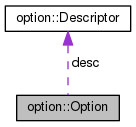
\includegraphics[width=174pt]{classoption_1_1Option__coll__graph}
\end{center}
\end{figure}
\subsection*{Public Member Functions}
\begin{DoxyCompactItemize}
\item 
int \hyperlink{classoption_1_1Option_a5268a69e1a91137186ab772574296da0}{type} () const
\begin{DoxyCompactList}\small\item\em Returns \hyperlink{structoption_1_1Descriptor_a1b220dabd8aad075fa441a80f9b9343c}{Descriptor\+::type} of this \hyperlink{classoption_1_1Option}{Option}\textquotesingle{}s \hyperlink{structoption_1_1Descriptor}{Descriptor}, or 0 if this \hyperlink{classoption_1_1Option}{Option} is invalid (unused). \end{DoxyCompactList}\item 
\mbox{\Hypertarget{classoption_1_1Option_a847d12e8e76add769fbd01c703e48682}\label{classoption_1_1Option_a847d12e8e76add769fbd01c703e48682}} 
int \hyperlink{classoption_1_1Option_a847d12e8e76add769fbd01c703e48682}{index} () const
\begin{DoxyCompactList}\small\item\em Returns \hyperlink{structoption_1_1Descriptor_a1fee8ac44f529c99ac2b1149b4c391b1}{Descriptor\+::index} of this \hyperlink{classoption_1_1Option}{Option}\textquotesingle{}s \hyperlink{structoption_1_1Descriptor}{Descriptor}, or -\/1 if this \hyperlink{classoption_1_1Option}{Option} is invalid (unused). \end{DoxyCompactList}\item 
int \hyperlink{classoption_1_1Option_a8a632dcd89af60fe0806deb756c08f14}{count} ()
\begin{DoxyCompactList}\small\item\em Returns the number of times this \hyperlink{classoption_1_1Option}{Option} (or others with the same \hyperlink{structoption_1_1Descriptor_a1fee8ac44f529c99ac2b1149b4c391b1}{Descriptor\+::index}) occurs in the argument vector. \end{DoxyCompactList}\item 
bool \hyperlink{classoption_1_1Option_af51f53a553ef46110e36008a58466a2e}{is\+First} () const
\begin{DoxyCompactList}\small\item\em Returns true iff this is the first element of the linked list. \end{DoxyCompactList}\item 
bool \hyperlink{classoption_1_1Option_a36fa8fde6fce89462ded79ab56180ff7}{is\+Last} () const
\begin{DoxyCompactList}\small\item\em Returns true iff this is the last element of the linked list. \end{DoxyCompactList}\item 
\hyperlink{classoption_1_1Option}{Option} $\ast$ \hyperlink{classoption_1_1Option_abb4e13cd7c90999c8a6b1f871cece283}{first} ()
\begin{DoxyCompactList}\small\item\em Returns a pointer to the first element of the linked list. \end{DoxyCompactList}\item 
\hyperlink{classoption_1_1Option}{Option} $\ast$ \hyperlink{classoption_1_1Option_afe2aff68191e55b59c53fac3dbbcd7c3}{last} ()
\begin{DoxyCompactList}\small\item\em Returns a pointer to the last element of the linked list. \end{DoxyCompactList}\item 
\hyperlink{classoption_1_1Option}{Option} $\ast$ \hyperlink{classoption_1_1Option_a4d12001a91b0b35cf47437d0c60d2b52}{prev} ()
\begin{DoxyCompactList}\small\item\em Returns a pointer to the previous element of the linked list or N\+U\+LL if called on \hyperlink{classoption_1_1Option_abb4e13cd7c90999c8a6b1f871cece283}{first()}. \end{DoxyCompactList}\item 
\hyperlink{classoption_1_1Option}{Option} $\ast$ \hyperlink{classoption_1_1Option_a1226e45dc2de30f269b2aff1784bbee7}{prevwrap} ()
\begin{DoxyCompactList}\small\item\em Returns a pointer to the previous element of the linked list with wrap-\/around from \hyperlink{classoption_1_1Option_abb4e13cd7c90999c8a6b1f871cece283}{first()} to \hyperlink{classoption_1_1Option_afe2aff68191e55b59c53fac3dbbcd7c3}{last()}. \end{DoxyCompactList}\item 
\hyperlink{classoption_1_1Option}{Option} $\ast$ \hyperlink{classoption_1_1Option_a59ae9aed505f4d410633bb36478a32be}{next} ()
\begin{DoxyCompactList}\small\item\em Returns a pointer to the next element of the linked list or N\+U\+LL if called on \hyperlink{classoption_1_1Option_afe2aff68191e55b59c53fac3dbbcd7c3}{last()}. \end{DoxyCompactList}\item 
\hyperlink{classoption_1_1Option}{Option} $\ast$ \hyperlink{classoption_1_1Option_ae8d8c058af3c781cb1d444998df48fef}{nextwrap} ()
\begin{DoxyCompactList}\small\item\em Returns a pointer to the next element of the linked list with wrap-\/around from \hyperlink{classoption_1_1Option_afe2aff68191e55b59c53fac3dbbcd7c3}{last()} to \hyperlink{classoption_1_1Option_abb4e13cd7c90999c8a6b1f871cece283}{first()}. \end{DoxyCompactList}\item 
void \hyperlink{classoption_1_1Option_a59030822a1ec4e667e6c288d7e5ec961}{append} (\hyperlink{classoption_1_1Option}{Option} $\ast$new\+\_\+last)
\begin{DoxyCompactList}\small\item\em Makes {\ttfamily new\+\_\+last} the new \hyperlink{classoption_1_1Option_afe2aff68191e55b59c53fac3dbbcd7c3}{last()} by chaining it into the list after \hyperlink{classoption_1_1Option_afe2aff68191e55b59c53fac3dbbcd7c3}{last()}. \end{DoxyCompactList}\item 
\hyperlink{classoption_1_1Option_a3c0504baaa809c622d59c2c09f83e25b}{operator const Option $\ast$} () const
\begin{DoxyCompactList}\small\item\em Casts from \hyperlink{classoption_1_1Option}{Option} to const Option$\ast$ but only if this \hyperlink{classoption_1_1Option}{Option} is valid. \end{DoxyCompactList}\item 
\hyperlink{classoption_1_1Option_ac5b9235d79208035d97e41fe17ba04d6}{operator Option $\ast$} ()
\begin{DoxyCompactList}\small\item\em Casts from \hyperlink{classoption_1_1Option}{Option} to Option$\ast$ but only if this \hyperlink{classoption_1_1Option}{Option} is valid. \end{DoxyCompactList}\item 
\mbox{\Hypertarget{classoption_1_1Option_aa2810152fc23b14175b115d1a7d38095}\label{classoption_1_1Option_aa2810152fc23b14175b115d1a7d38095}} 
\hyperlink{classoption_1_1Option_aa2810152fc23b14175b115d1a7d38095}{Option} ()
\begin{DoxyCompactList}\small\item\em Creates a new \hyperlink{classoption_1_1Option}{Option} that is a one-\/element linked list and has N\+U\+LL \hyperlink{classoption_1_1Option_af8d664a7b5de1425008b1812a90a0c23}{desc}, \hyperlink{classoption_1_1Option_a02a76b4896abd22d0ba8514362261de9}{name}, \hyperlink{classoption_1_1Option_a402be734987458364b0f473acae36238}{arg} and \hyperlink{classoption_1_1Option_a3aa2957b19ad5815873441b415d56050}{namelen}. \end{DoxyCompactList}\item 
\hyperlink{classoption_1_1Option_a385221e2a8f37c548f0d5777bfddb216}{Option} (const \hyperlink{structoption_1_1Descriptor}{Descriptor} $\ast$desc\+\_\+, const char $\ast$name\+\_\+, const char $\ast$arg\+\_\+)
\begin{DoxyCompactList}\small\item\em Creates a new \hyperlink{classoption_1_1Option}{Option} that is a one-\/element linked list and has the given values for \hyperlink{classoption_1_1Option_af8d664a7b5de1425008b1812a90a0c23}{desc}, \hyperlink{classoption_1_1Option_a02a76b4896abd22d0ba8514362261de9}{name} and \hyperlink{classoption_1_1Option_a402be734987458364b0f473acae36238}{arg}. \end{DoxyCompactList}\item 
void \hyperlink{classoption_1_1Option_adb4b44f3778df8f28a04c48bd1b4a72b}{operator=} (const \hyperlink{classoption_1_1Option}{Option} \&orig)
\begin{DoxyCompactList}\small\item\em Makes {\ttfamily $\ast$this} a copy of {\ttfamily orig} except for the linked list pointers. \end{DoxyCompactList}\item 
\hyperlink{classoption_1_1Option_a4053240fecad1a3b1d8e4dc06b7aa8c4}{Option} (const \hyperlink{classoption_1_1Option}{Option} \&orig)
\begin{DoxyCompactList}\small\item\em Makes {\ttfamily $\ast$this} a copy of {\ttfamily orig} except for the linked list pointers. \end{DoxyCompactList}\end{DoxyCompactItemize}
\subsection*{Public Attributes}
\begin{DoxyCompactItemize}
\item 
const \hyperlink{structoption_1_1Descriptor}{Descriptor} $\ast$ \hyperlink{classoption_1_1Option_af8d664a7b5de1425008b1812a90a0c23}{desc}
\begin{DoxyCompactList}\small\item\em Pointer to this \hyperlink{classoption_1_1Option}{Option}\textquotesingle{}s \hyperlink{structoption_1_1Descriptor}{Descriptor}. \end{DoxyCompactList}\item 
const char $\ast$ \hyperlink{classoption_1_1Option_a02a76b4896abd22d0ba8514362261de9}{name}
\begin{DoxyCompactList}\small\item\em The name of the option as used on the command line. \end{DoxyCompactList}\item 
const char $\ast$ \hyperlink{classoption_1_1Option_a402be734987458364b0f473acae36238}{arg}
\begin{DoxyCompactList}\small\item\em Pointer to this \hyperlink{classoption_1_1Option}{Option}\textquotesingle{}s argument (if any). \end{DoxyCompactList}\item 
int \hyperlink{classoption_1_1Option_a3aa2957b19ad5815873441b415d56050}{namelen}
\begin{DoxyCompactList}\small\item\em The length of the option \hyperlink{classoption_1_1Option_a02a76b4896abd22d0ba8514362261de9}{name}. \end{DoxyCompactList}\end{DoxyCompactItemize}


\subsection{Detailed Description}
A parsed option from the command line together with its argument if it has one. 

The \hyperlink{classoption_1_1Parser}{Parser} chains all parsed options with the same \hyperlink{structoption_1_1Descriptor_a1fee8ac44f529c99ac2b1149b4c391b1}{Descriptor\+::index} together to form a linked list. This allows you to easily implement all of the common ways of handling repeated options and enable/disable pairs.

\begin{DoxyItemize}
\item Test for presence of a switch in the argument vector\+: 
\begin{DoxyCode}
\textcolor{keywordflow}{if} ( options[QUIET] ) ... 
\end{DoxyCode}
 \item Evaluate --enable-\/foo/--disable-\/foo pair where the last one used wins\+: 
\begin{DoxyCode}
\textcolor{keywordflow}{if} ( options[FOO].\hyperlink{classoption_1_1Option_afe2aff68191e55b59c53fac3dbbcd7c3}{last}()->\hyperlink{classoption_1_1Option_a5268a69e1a91137186ab772574296da0}{type}() == DISABLE ) ... 
\end{DoxyCode}
 \item Cumulative option (-\/v verbose, -\/vv more verbose, -\/vvv even more verbose)\+: 
\begin{DoxyCode}
\textcolor{keywordtype}{int} verbosity = options[VERBOSE].\hyperlink{classoption_1_1Option_a8a632dcd89af60fe0806deb756c08f14}{count}(); 
\end{DoxyCode}
 \item Iterate over all --file=$<$fname$>$ arguments\+: 
\begin{DoxyCode}
\textcolor{keywordflow}{for} (\hyperlink{classoption_1_1Option_aa2810152fc23b14175b115d1a7d38095}{Option}* opt = options[FILE]; opt; opt = opt->\hyperlink{classoption_1_1Option_a59ae9aed505f4d410633bb36478a32be}{next}())
 fname = opt->arg; ... 
\end{DoxyCode}
 \end{DoxyItemize}


\subsection{Constructor \& Destructor Documentation}
\mbox{\Hypertarget{classoption_1_1Option_a385221e2a8f37c548f0d5777bfddb216}\label{classoption_1_1Option_a385221e2a8f37c548f0d5777bfddb216}} 
\index{option\+::\+Option@{option\+::\+Option}!Option@{Option}}
\index{Option@{Option}!option\+::\+Option@{option\+::\+Option}}
\subsubsection{\texorpdfstring{Option()}{Option()}\hspace{0.1cm}{\footnotesize\ttfamily [1/2]}}
{\footnotesize\ttfamily option\+::\+Option\+::\+Option (\begin{DoxyParamCaption}\item[{const \hyperlink{structoption_1_1Descriptor}{Descriptor} $\ast$}]{desc\+\_\+,  }\item[{const char $\ast$}]{name\+\_\+,  }\item[{const char $\ast$}]{arg\+\_\+ }\end{DoxyParamCaption})\hspace{0.3cm}{\ttfamily [inline]}}



Creates a new \hyperlink{classoption_1_1Option}{Option} that is a one-\/element linked list and has the given values for \hyperlink{classoption_1_1Option_af8d664a7b5de1425008b1812a90a0c23}{desc}, \hyperlink{classoption_1_1Option_a02a76b4896abd22d0ba8514362261de9}{name} and \hyperlink{classoption_1_1Option_a402be734987458364b0f473acae36238}{arg}. 

If {\ttfamily name\+\_\+} points at a character other than \textquotesingle{}-\/\textquotesingle{} it will be assumed to refer to a short option and \hyperlink{classoption_1_1Option_a3aa2957b19ad5815873441b415d56050}{namelen} will be set to 1. Otherwise the length will extend to the first \textquotesingle{}=\textquotesingle{} character or the string\textquotesingle{}s 0-\/terminator. \mbox{\Hypertarget{classoption_1_1Option_a4053240fecad1a3b1d8e4dc06b7aa8c4}\label{classoption_1_1Option_a4053240fecad1a3b1d8e4dc06b7aa8c4}} 
\index{option\+::\+Option@{option\+::\+Option}!Option@{Option}}
\index{Option@{Option}!option\+::\+Option@{option\+::\+Option}}
\subsubsection{\texorpdfstring{Option()}{Option()}\hspace{0.1cm}{\footnotesize\ttfamily [2/2]}}
{\footnotesize\ttfamily option\+::\+Option\+::\+Option (\begin{DoxyParamCaption}\item[{const \hyperlink{classoption_1_1Option}{Option} \&}]{orig }\end{DoxyParamCaption})\hspace{0.3cm}{\ttfamily [inline]}}



Makes {\ttfamily $\ast$this} a copy of {\ttfamily orig} except for the linked list pointers. 

After this operation {\ttfamily $\ast$this} will be a one-\/element linked list. 

\subsection{Member Function Documentation}
\mbox{\Hypertarget{classoption_1_1Option_a59030822a1ec4e667e6c288d7e5ec961}\label{classoption_1_1Option_a59030822a1ec4e667e6c288d7e5ec961}} 
\index{option\+::\+Option@{option\+::\+Option}!append@{append}}
\index{append@{append}!option\+::\+Option@{option\+::\+Option}}
\subsubsection{\texorpdfstring{append()}{append()}}
{\footnotesize\ttfamily void option\+::\+Option\+::append (\begin{DoxyParamCaption}\item[{\hyperlink{classoption_1_1Option}{Option} $\ast$}]{new\+\_\+last }\end{DoxyParamCaption})\hspace{0.3cm}{\ttfamily [inline]}}



Makes {\ttfamily new\+\_\+last} the new \hyperlink{classoption_1_1Option_afe2aff68191e55b59c53fac3dbbcd7c3}{last()} by chaining it into the list after \hyperlink{classoption_1_1Option_afe2aff68191e55b59c53fac3dbbcd7c3}{last()}. 

It doesn\textquotesingle{}t matter which element you call \hyperlink{classoption_1_1Option_a59030822a1ec4e667e6c288d7e5ec961}{append()} on. The new element will always be appended to \hyperlink{classoption_1_1Option_afe2aff68191e55b59c53fac3dbbcd7c3}{last()}.

\begin{DoxyAttention}{Attention}
{\ttfamily new\+\_\+last} must not yet be part of a list, or that list will become corrupted, because this method does not unchain {\ttfamily new\+\_\+last} from an existing list. 
\end{DoxyAttention}
\mbox{\Hypertarget{classoption_1_1Option_a8a632dcd89af60fe0806deb756c08f14}\label{classoption_1_1Option_a8a632dcd89af60fe0806deb756c08f14}} 
\index{option\+::\+Option@{option\+::\+Option}!count@{count}}
\index{count@{count}!option\+::\+Option@{option\+::\+Option}}
\subsubsection{\texorpdfstring{count()}{count()}}
{\footnotesize\ttfamily int option\+::\+Option\+::count (\begin{DoxyParamCaption}{ }\end{DoxyParamCaption})\hspace{0.3cm}{\ttfamily [inline]}}



Returns the number of times this \hyperlink{classoption_1_1Option}{Option} (or others with the same \hyperlink{structoption_1_1Descriptor_a1fee8ac44f529c99ac2b1149b4c391b1}{Descriptor\+::index}) occurs in the argument vector. 

This corresponds to the number of elements in the linked list this \hyperlink{classoption_1_1Option}{Option} is part of. It doesn\textquotesingle{}t matter on which element you call \hyperlink{classoption_1_1Option_a8a632dcd89af60fe0806deb756c08f14}{count()}. The return value is always the same.

Use this to implement cumulative options, such as -\/v, -\/vv, -\/vvv for different verbosity levels.

Returns 0 when called for an unused/invalid option. \mbox{\Hypertarget{classoption_1_1Option_abb4e13cd7c90999c8a6b1f871cece283}\label{classoption_1_1Option_abb4e13cd7c90999c8a6b1f871cece283}} 
\index{option\+::\+Option@{option\+::\+Option}!first@{first}}
\index{first@{first}!option\+::\+Option@{option\+::\+Option}}
\subsubsection{\texorpdfstring{first()}{first()}}
{\footnotesize\ttfamily \hyperlink{classoption_1_1Option}{Option}$\ast$ option\+::\+Option\+::first (\begin{DoxyParamCaption}{ }\end{DoxyParamCaption})\hspace{0.3cm}{\ttfamily [inline]}}



Returns a pointer to the first element of the linked list. 

Use this when you want the first occurrence of an option on the command line to take precedence. Note that this is not the way most programs handle options. You should probably be using \hyperlink{classoption_1_1Option_afe2aff68191e55b59c53fac3dbbcd7c3}{last()} instead.

\begin{DoxyNote}{Note}
This method may be called on an unused/invalid option and will return a pointer to the option itself. 
\end{DoxyNote}
\mbox{\Hypertarget{classoption_1_1Option_af51f53a553ef46110e36008a58466a2e}\label{classoption_1_1Option_af51f53a553ef46110e36008a58466a2e}} 
\index{option\+::\+Option@{option\+::\+Option}!is\+First@{is\+First}}
\index{is\+First@{is\+First}!option\+::\+Option@{option\+::\+Option}}
\subsubsection{\texorpdfstring{is\+First()}{isFirst()}}
{\footnotesize\ttfamily bool option\+::\+Option\+::is\+First (\begin{DoxyParamCaption}{ }\end{DoxyParamCaption}) const\hspace{0.3cm}{\ttfamily [inline]}}



Returns true iff this is the first element of the linked list. 

The first element in the linked list is the first option on the command line that has the respective \hyperlink{structoption_1_1Descriptor_a1fee8ac44f529c99ac2b1149b4c391b1}{Descriptor\+::index} value.

Returns true for an unused/invalid option. \mbox{\Hypertarget{classoption_1_1Option_a36fa8fde6fce89462ded79ab56180ff7}\label{classoption_1_1Option_a36fa8fde6fce89462ded79ab56180ff7}} 
\index{option\+::\+Option@{option\+::\+Option}!is\+Last@{is\+Last}}
\index{is\+Last@{is\+Last}!option\+::\+Option@{option\+::\+Option}}
\subsubsection{\texorpdfstring{is\+Last()}{isLast()}}
{\footnotesize\ttfamily bool option\+::\+Option\+::is\+Last (\begin{DoxyParamCaption}{ }\end{DoxyParamCaption}) const\hspace{0.3cm}{\ttfamily [inline]}}



Returns true iff this is the last element of the linked list. 

The last element in the linked list is the last option on the command line that has the respective \hyperlink{structoption_1_1Descriptor_a1fee8ac44f529c99ac2b1149b4c391b1}{Descriptor\+::index} value.

Returns true for an unused/invalid option. \mbox{\Hypertarget{classoption_1_1Option_afe2aff68191e55b59c53fac3dbbcd7c3}\label{classoption_1_1Option_afe2aff68191e55b59c53fac3dbbcd7c3}} 
\index{option\+::\+Option@{option\+::\+Option}!last@{last}}
\index{last@{last}!option\+::\+Option@{option\+::\+Option}}
\subsubsection{\texorpdfstring{last()}{last()}}
{\footnotesize\ttfamily \hyperlink{classoption_1_1Option}{Option}$\ast$ option\+::\+Option\+::last (\begin{DoxyParamCaption}{ }\end{DoxyParamCaption})\hspace{0.3cm}{\ttfamily [inline]}}



Returns a pointer to the last element of the linked list. 

Use this when you want the last occurrence of an option on the command line to take precedence. This is the most common way of handling conflicting options.

\begin{DoxyNote}{Note}
This method may be called on an unused/invalid option and will return a pointer to the option itself.
\end{DoxyNote}
\begin{DoxyParagraph}{Tip\+:}
If you have options with opposite meanings (e.\+g. {\ttfamily --enable-\/foo} and {\ttfamily --disable-\/foo}), you can assign them the same \hyperlink{structoption_1_1Descriptor_a1fee8ac44f529c99ac2b1149b4c391b1}{Descriptor\+::index} to get them into the same list. Distinguish them by \hyperlink{structoption_1_1Descriptor_a1b220dabd8aad075fa441a80f9b9343c}{Descriptor\+::type} and all you have to do is check {\ttfamily  \hyperlink{classoption_1_1Option_afe2aff68191e55b59c53fac3dbbcd7c3}{last()}-\/$>$\hyperlink{classoption_1_1Option_a5268a69e1a91137186ab772574296da0}{type()} } to get the state listed last on the command line. 
\end{DoxyParagraph}
\mbox{\Hypertarget{classoption_1_1Option_a59ae9aed505f4d410633bb36478a32be}\label{classoption_1_1Option_a59ae9aed505f4d410633bb36478a32be}} 
\index{option\+::\+Option@{option\+::\+Option}!next@{next}}
\index{next@{next}!option\+::\+Option@{option\+::\+Option}}
\subsubsection{\texorpdfstring{next()}{next()}}
{\footnotesize\ttfamily \hyperlink{classoption_1_1Option}{Option}$\ast$ option\+::\+Option\+::next (\begin{DoxyParamCaption}{ }\end{DoxyParamCaption})\hspace{0.3cm}{\ttfamily [inline]}}



Returns a pointer to the next element of the linked list or N\+U\+LL if called on \hyperlink{classoption_1_1Option_afe2aff68191e55b59c53fac3dbbcd7c3}{last()}. 

If called on \hyperlink{classoption_1_1Option_afe2aff68191e55b59c53fac3dbbcd7c3}{last()} this method returns N\+U\+LL. Otherwise it will return the option with the same \hyperlink{structoption_1_1Descriptor_a1fee8ac44f529c99ac2b1149b4c391b1}{Descriptor\+::index} that follows this option on the command line. \mbox{\Hypertarget{classoption_1_1Option_ae8d8c058af3c781cb1d444998df48fef}\label{classoption_1_1Option_ae8d8c058af3c781cb1d444998df48fef}} 
\index{option\+::\+Option@{option\+::\+Option}!nextwrap@{nextwrap}}
\index{nextwrap@{nextwrap}!option\+::\+Option@{option\+::\+Option}}
\subsubsection{\texorpdfstring{nextwrap()}{nextwrap()}}
{\footnotesize\ttfamily \hyperlink{classoption_1_1Option}{Option}$\ast$ option\+::\+Option\+::nextwrap (\begin{DoxyParamCaption}{ }\end{DoxyParamCaption})\hspace{0.3cm}{\ttfamily [inline]}}



Returns a pointer to the next element of the linked list with wrap-\/around from \hyperlink{classoption_1_1Option_afe2aff68191e55b59c53fac3dbbcd7c3}{last()} to \hyperlink{classoption_1_1Option_abb4e13cd7c90999c8a6b1f871cece283}{first()}. 

If called on \hyperlink{classoption_1_1Option_afe2aff68191e55b59c53fac3dbbcd7c3}{last()} this method returns \hyperlink{classoption_1_1Option_abb4e13cd7c90999c8a6b1f871cece283}{first()}. Otherwise it will return the option with the same \hyperlink{structoption_1_1Descriptor_a1fee8ac44f529c99ac2b1149b4c391b1}{Descriptor\+::index} that follows this option on the command line. \mbox{\Hypertarget{classoption_1_1Option_a3c0504baaa809c622d59c2c09f83e25b}\label{classoption_1_1Option_a3c0504baaa809c622d59c2c09f83e25b}} 
\index{option\+::\+Option@{option\+::\+Option}!operator const Option $\ast$@{operator const Option $\ast$}}
\index{operator const Option $\ast$@{operator const Option $\ast$}!option\+::\+Option@{option\+::\+Option}}
\subsubsection{\texorpdfstring{operator const Option $\ast$()}{operator const Option *()}}
{\footnotesize\ttfamily option\+::\+Option\+::operator const \hyperlink{classoption_1_1Option}{Option} $\ast$ (\begin{DoxyParamCaption}{ }\end{DoxyParamCaption}) const\hspace{0.3cm}{\ttfamily [inline]}}



Casts from \hyperlink{classoption_1_1Option}{Option} to const Option$\ast$ but only if this \hyperlink{classoption_1_1Option}{Option} is valid. 

If this \hyperlink{classoption_1_1Option}{Option} is valid (i.\+e. {\ttfamily desc!=N\+U\+LL}), returns this. Otherwise returns N\+U\+LL. This allows testing an \hyperlink{classoption_1_1Option}{Option} directly in an if-\/clause to see if it is used\+: 
\begin{DoxyCode}
\textcolor{keywordflow}{if} (options[CREATE])
\{
  ...
\}
\end{DoxyCode}
 It also allows you to write loops like this\+: 
\begin{DoxyCode}
\textcolor{keywordflow}{for} (\hyperlink{classoption_1_1Option_aa2810152fc23b14175b115d1a7d38095}{Option}* opt = options[FILE]; opt; opt = opt->\hyperlink{classoption_1_1Option_a59ae9aed505f4d410633bb36478a32be}{next}())
 fname = opt->arg; ... 
\end{DoxyCode}
 \mbox{\Hypertarget{classoption_1_1Option_ac5b9235d79208035d97e41fe17ba04d6}\label{classoption_1_1Option_ac5b9235d79208035d97e41fe17ba04d6}} 
\index{option\+::\+Option@{option\+::\+Option}!operator Option $\ast$@{operator Option $\ast$}}
\index{operator Option $\ast$@{operator Option $\ast$}!option\+::\+Option@{option\+::\+Option}}
\subsubsection{\texorpdfstring{operator Option $\ast$()}{operator Option *()}}
{\footnotesize\ttfamily option\+::\+Option\+::operator \hyperlink{classoption_1_1Option}{Option} $\ast$ (\begin{DoxyParamCaption}{ }\end{DoxyParamCaption})\hspace{0.3cm}{\ttfamily [inline]}}



Casts from \hyperlink{classoption_1_1Option}{Option} to Option$\ast$ but only if this \hyperlink{classoption_1_1Option}{Option} is valid. 

If this \hyperlink{classoption_1_1Option}{Option} is valid (i.\+e. {\ttfamily desc!=N\+U\+LL}), returns this. Otherwise returns N\+U\+LL. This allows testing an \hyperlink{classoption_1_1Option}{Option} directly in an if-\/clause to see if it is used\+: 
\begin{DoxyCode}
\textcolor{keywordflow}{if} (options[CREATE])
\{
  ...
\}
\end{DoxyCode}
 It also allows you to write loops like this\+: 
\begin{DoxyCode}
\textcolor{keywordflow}{for} (\hyperlink{classoption_1_1Option_aa2810152fc23b14175b115d1a7d38095}{Option}* opt = options[FILE]; opt; opt = opt->\hyperlink{classoption_1_1Option_a59ae9aed505f4d410633bb36478a32be}{next}())
 fname = opt->arg; ... 
\end{DoxyCode}
 \mbox{\Hypertarget{classoption_1_1Option_adb4b44f3778df8f28a04c48bd1b4a72b}\label{classoption_1_1Option_adb4b44f3778df8f28a04c48bd1b4a72b}} 
\index{option\+::\+Option@{option\+::\+Option}!operator=@{operator=}}
\index{operator=@{operator=}!option\+::\+Option@{option\+::\+Option}}
\subsubsection{\texorpdfstring{operator=()}{operator=()}}
{\footnotesize\ttfamily void option\+::\+Option\+::operator= (\begin{DoxyParamCaption}\item[{const \hyperlink{classoption_1_1Option}{Option} \&}]{orig }\end{DoxyParamCaption})\hspace{0.3cm}{\ttfamily [inline]}}



Makes {\ttfamily $\ast$this} a copy of {\ttfamily orig} except for the linked list pointers. 

After this operation {\ttfamily $\ast$this} will be a one-\/element linked list. \mbox{\Hypertarget{classoption_1_1Option_a4d12001a91b0b35cf47437d0c60d2b52}\label{classoption_1_1Option_a4d12001a91b0b35cf47437d0c60d2b52}} 
\index{option\+::\+Option@{option\+::\+Option}!prev@{prev}}
\index{prev@{prev}!option\+::\+Option@{option\+::\+Option}}
\subsubsection{\texorpdfstring{prev()}{prev()}}
{\footnotesize\ttfamily \hyperlink{classoption_1_1Option}{Option}$\ast$ option\+::\+Option\+::prev (\begin{DoxyParamCaption}{ }\end{DoxyParamCaption})\hspace{0.3cm}{\ttfamily [inline]}}



Returns a pointer to the previous element of the linked list or N\+U\+LL if called on \hyperlink{classoption_1_1Option_abb4e13cd7c90999c8a6b1f871cece283}{first()}. 

If called on \hyperlink{classoption_1_1Option_abb4e13cd7c90999c8a6b1f871cece283}{first()} this method returns N\+U\+LL. Otherwise it will return the option with the same \hyperlink{structoption_1_1Descriptor_a1fee8ac44f529c99ac2b1149b4c391b1}{Descriptor\+::index} that precedes this option on the command line. \mbox{\Hypertarget{classoption_1_1Option_a1226e45dc2de30f269b2aff1784bbee7}\label{classoption_1_1Option_a1226e45dc2de30f269b2aff1784bbee7}} 
\index{option\+::\+Option@{option\+::\+Option}!prevwrap@{prevwrap}}
\index{prevwrap@{prevwrap}!option\+::\+Option@{option\+::\+Option}}
\subsubsection{\texorpdfstring{prevwrap()}{prevwrap()}}
{\footnotesize\ttfamily \hyperlink{classoption_1_1Option}{Option}$\ast$ option\+::\+Option\+::prevwrap (\begin{DoxyParamCaption}{ }\end{DoxyParamCaption})\hspace{0.3cm}{\ttfamily [inline]}}



Returns a pointer to the previous element of the linked list with wrap-\/around from \hyperlink{classoption_1_1Option_abb4e13cd7c90999c8a6b1f871cece283}{first()} to \hyperlink{classoption_1_1Option_afe2aff68191e55b59c53fac3dbbcd7c3}{last()}. 

If called on \hyperlink{classoption_1_1Option_abb4e13cd7c90999c8a6b1f871cece283}{first()} this method returns \hyperlink{classoption_1_1Option_afe2aff68191e55b59c53fac3dbbcd7c3}{last()}. Otherwise it will return the option with the same \hyperlink{structoption_1_1Descriptor_a1fee8ac44f529c99ac2b1149b4c391b1}{Descriptor\+::index} that precedes this option on the command line. \mbox{\Hypertarget{classoption_1_1Option_a5268a69e1a91137186ab772574296da0}\label{classoption_1_1Option_a5268a69e1a91137186ab772574296da0}} 
\index{option\+::\+Option@{option\+::\+Option}!type@{type}}
\index{type@{type}!option\+::\+Option@{option\+::\+Option}}
\subsubsection{\texorpdfstring{type()}{type()}}
{\footnotesize\ttfamily int option\+::\+Option\+::type (\begin{DoxyParamCaption}{ }\end{DoxyParamCaption}) const\hspace{0.3cm}{\ttfamily [inline]}}



Returns \hyperlink{structoption_1_1Descriptor_a1b220dabd8aad075fa441a80f9b9343c}{Descriptor\+::type} of this \hyperlink{classoption_1_1Option}{Option}\textquotesingle{}s \hyperlink{structoption_1_1Descriptor}{Descriptor}, or 0 if this \hyperlink{classoption_1_1Option}{Option} is invalid (unused). 

Because this method (and \hyperlink{classoption_1_1Option_afe2aff68191e55b59c53fac3dbbcd7c3}{last()}, too) can be used even on unused Options with desc==0, you can (provided you arrange your types properly) switch on \hyperlink{classoption_1_1Option_a5268a69e1a91137186ab772574296da0}{type()} without testing validity first. 
\begin{DoxyCode}
\textcolor{keyword}{enum} OptionType \{ UNUSED=0, DISABLED=0, ENABLED=1 \};
\textcolor{keyword}{enum} OptionIndex \{ FOO \};
\textcolor{keyword}{const} Descriptor usage[] = \{
  \{ FOO, ENABLED,  \textcolor{stringliteral}{""}, \textcolor{stringliteral}{"enable-foo"},  \hyperlink{structoption_1_1Arg_a7fc01987899c91c6b6a1be5711a46e22}{Arg::None}, 0 \},
  \{ FOO, DISABLED, \textcolor{stringliteral}{""}, \textcolor{stringliteral}{"disable-foo"}, \hyperlink{structoption_1_1Arg_a7fc01987899c91c6b6a1be5711a46e22}{Arg::None}, 0 \},
  \{ 0, 0, 0, 0, 0, 0 \} \};
...
switch(options[FOO].\hyperlink{classoption_1_1Option_afe2aff68191e55b59c53fac3dbbcd7c3}{last}()->\hyperlink{classoption_1_1Option_a5268a69e1a91137186ab772574296da0}{type}()) \textcolor{comment}{// no validity check required!}
\{
  \textcolor{keywordflow}{case} ENABLED: ...
  \textcolor{keywordflow}{case} DISABLED: ...  \textcolor{comment}{// UNUSED==DISABLED !}
\}
\end{DoxyCode}
 

\subsection{Member Data Documentation}
\mbox{\Hypertarget{classoption_1_1Option_a402be734987458364b0f473acae36238}\label{classoption_1_1Option_a402be734987458364b0f473acae36238}} 
\index{option\+::\+Option@{option\+::\+Option}!arg@{arg}}
\index{arg@{arg}!option\+::\+Option@{option\+::\+Option}}
\subsubsection{\texorpdfstring{arg}{arg}}
{\footnotesize\ttfamily const char$\ast$ option\+::\+Option\+::arg}



Pointer to this \hyperlink{classoption_1_1Option}{Option}\textquotesingle{}s argument (if any). 

N\+U\+LL if this option has no argument. Do not confuse this with the empty string which is a valid argument. \mbox{\Hypertarget{classoption_1_1Option_af8d664a7b5de1425008b1812a90a0c23}\label{classoption_1_1Option_af8d664a7b5de1425008b1812a90a0c23}} 
\index{option\+::\+Option@{option\+::\+Option}!desc@{desc}}
\index{desc@{desc}!option\+::\+Option@{option\+::\+Option}}
\subsubsection{\texorpdfstring{desc}{desc}}
{\footnotesize\ttfamily const \hyperlink{structoption_1_1Descriptor}{Descriptor}$\ast$ option\+::\+Option\+::desc}



Pointer to this \hyperlink{classoption_1_1Option}{Option}\textquotesingle{}s \hyperlink{structoption_1_1Descriptor}{Descriptor}. 

Remember that the first dummy descriptor (see \hyperlink{structoption_1_1Descriptor_a470c449dfa894c9bfda2dae026142b4b}{Descriptor\+::longopt}) is used for unknown options.

\begin{DoxyAttention}{Attention}
{\ttfamily desc==N\+U\+LL} signals that this \hyperlink{classoption_1_1Option}{Option} is unused. This is the default state of elements in the result array. You don\textquotesingle{}t need to test {\ttfamily desc} explicitly. You can simply write something like this\+: 
\begin{DoxyCode}
\textcolor{keywordflow}{if} (options[CREATE])
\{
  ...
\}
\end{DoxyCode}
 This works because of {\ttfamily  operator const Option$\ast$() }. 
\end{DoxyAttention}
\mbox{\Hypertarget{classoption_1_1Option_a02a76b4896abd22d0ba8514362261de9}\label{classoption_1_1Option_a02a76b4896abd22d0ba8514362261de9}} 
\index{option\+::\+Option@{option\+::\+Option}!name@{name}}
\index{name@{name}!option\+::\+Option@{option\+::\+Option}}
\subsubsection{\texorpdfstring{name}{name}}
{\footnotesize\ttfamily const char$\ast$ option\+::\+Option\+::name}



The name of the option as used on the command line. 

The main purpose of this string is to be presented to the user in messages.

In the case of a long option, this is the actual {\ttfamily argv} pointer, i.\+e. the first character is a \textquotesingle{}-\/\textquotesingle{}. In the case of a short option this points to the option character within the {\ttfamily argv} string.

Note that in the case of a short option group or an attached option argument, this string will contain additional characters following the actual name. Use \hyperlink{classoption_1_1Option_a3aa2957b19ad5815873441b415d56050}{namelen} to filter out the actual option name only. \mbox{\Hypertarget{classoption_1_1Option_a3aa2957b19ad5815873441b415d56050}\label{classoption_1_1Option_a3aa2957b19ad5815873441b415d56050}} 
\index{option\+::\+Option@{option\+::\+Option}!namelen@{namelen}}
\index{namelen@{namelen}!option\+::\+Option@{option\+::\+Option}}
\subsubsection{\texorpdfstring{namelen}{namelen}}
{\footnotesize\ttfamily int option\+::\+Option\+::namelen}



The length of the option \hyperlink{classoption_1_1Option_a02a76b4896abd22d0ba8514362261de9}{name}. 

Because \hyperlink{classoption_1_1Option_a02a76b4896abd22d0ba8514362261de9}{name} points into the actual {\ttfamily argv} string, the option name may be followed by more characters (e.\+g. other short options in the same short option group). This value is the number of bytes (not characters!) that are part of the actual name.

For a short option, this length is always 1. For a long option this length is always at least 2 if single minus long options are permitted and at least 3 if they are disabled.

\begin{DoxyNote}{Note}
In the pathological case of a minus within a short option group (e.\+g. {\ttfamily -\/xf-\/z}), this length is incorrect, because this case will be misinterpreted as a long option and the name will therefore extend to the string\textquotesingle{}s 0-\/terminator or a following \textquotesingle{}=" character if there is one. This is irrelevant for most uses of \hyperlink{classoption_1_1Option_a02a76b4896abd22d0ba8514362261de9}{name} and {\ttfamily namelen}. If you really need to distinguish the case of a long and a short option, compare \hyperlink{classoption_1_1Option_a02a76b4896abd22d0ba8514362261de9}{name} to the {\ttfamily argv} pointers. A long option\textquotesingle{}s {\ttfamily name} is always identical to one of them, whereas a short option\textquotesingle{}s is never. 
\end{DoxyNote}


The documentation for this class was generated from the following file\+:\begin{DoxyCompactItemize}
\item 
\hyperlink{optionparser_8h}{optionparser.\+h}\end{DoxyCompactItemize}

\hypertarget{structoption_1_1PrintUsageImplementation_1_1OStreamWriter}{}\section{option\+:\+:Print\+Usage\+Implementation\+:\+:O\+Stream\+Writer$<$ O\+Stream $>$ Struct Template Reference}
\label{structoption_1_1PrintUsageImplementation_1_1OStreamWriter}\index{option\+::\+Print\+Usage\+Implementation\+::\+O\+Stream\+Writer$<$ O\+Stream $>$@{option\+::\+Print\+Usage\+Implementation\+::\+O\+Stream\+Writer$<$ O\+Stream $>$}}


Inheritance diagram for option\+:\+:Print\+Usage\+Implementation\+:\+:O\+Stream\+Writer$<$ O\+Stream $>$\+:
\nopagebreak
\begin{figure}[H]
\begin{center}
\leavevmode
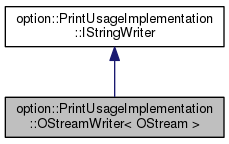
\includegraphics[width=244pt]{structoption_1_1PrintUsageImplementation_1_1OStreamWriter__inherit__graph}
\end{center}
\end{figure}


Collaboration diagram for option\+:\+:Print\+Usage\+Implementation\+:\+:O\+Stream\+Writer$<$ O\+Stream $>$\+:
\nopagebreak
\begin{figure}[H]
\begin{center}
\leavevmode
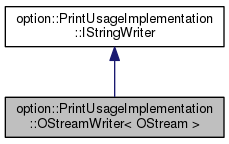
\includegraphics[width=244pt]{structoption_1_1PrintUsageImplementation_1_1OStreamWriter__coll__graph}
\end{center}
\end{figure}
\subsection*{Public Member Functions}
\begin{DoxyCompactItemize}
\item 
virtual void \hyperlink{structoption_1_1PrintUsageImplementation_1_1OStreamWriter_a323890fba123ad476fa2471029fc7b23}{operator()} (const char $\ast$str, int size)\hypertarget{structoption_1_1PrintUsageImplementation_1_1OStreamWriter_a323890fba123ad476fa2471029fc7b23}{}\label{structoption_1_1PrintUsageImplementation_1_1OStreamWriter_a323890fba123ad476fa2471029fc7b23}

\begin{DoxyCompactList}\small\item\em Writes the given number of chars beginning at the given pointer somewhere. \end{DoxyCompactList}\item 
{\bfseries O\+Stream\+Writer} (O\+Stream \&o)\hypertarget{structoption_1_1PrintUsageImplementation_1_1OStreamWriter_abf38eb181267e96d86de1ea09ad22c3f}{}\label{structoption_1_1PrintUsageImplementation_1_1OStreamWriter_abf38eb181267e96d86de1ea09ad22c3f}

\end{DoxyCompactItemize}
\subsection*{Public Attributes}
\begin{DoxyCompactItemize}
\item 
O\+Stream \& {\bfseries ostream}\hypertarget{structoption_1_1PrintUsageImplementation_1_1OStreamWriter_a9b808696e204a834acd4362c62b9f4c1}{}\label{structoption_1_1PrintUsageImplementation_1_1OStreamWriter_a9b808696e204a834acd4362c62b9f4c1}

\end{DoxyCompactItemize}


The documentation for this struct was generated from the following file\+:\begin{DoxyCompactItemize}
\item 
\hyperlink{optionparser_8h}{optionparser.\+h}\end{DoxyCompactItemize}

\hypertarget{classoption_1_1Parser}{}\section{option\+:\+:Parser Class Reference}
\label{classoption_1_1Parser}\index{option\+::\+Parser@{option\+::\+Parser}}


Checks argument vectors for validity and parses them into data structures that are easier to work with.  




{\ttfamily \#include $<$optionparser.\+h$>$}

\subsection*{Classes}
\begin{DoxyCompactItemize}
\item 
struct \hyperlink{structoption_1_1Parser_1_1Action}{Action}
\item 
class \hyperlink{classoption_1_1Parser_1_1StoreOptionAction}{Store\+Option\+Action}
\end{DoxyCompactItemize}
\subsection*{Public Member Functions}
\begin{DoxyCompactItemize}
\item 
\mbox{\Hypertarget{classoption_1_1Parser_a895e9a1db19f1a026ee6a7412de17d04}\label{classoption_1_1Parser_a895e9a1db19f1a026ee6a7412de17d04}} 
\hyperlink{classoption_1_1Parser_a895e9a1db19f1a026ee6a7412de17d04}{Parser} ()
\begin{DoxyCompactList}\small\item\em Creates a new \hyperlink{classoption_1_1Parser}{Parser}. \end{DoxyCompactList}\item 
\hyperlink{classoption_1_1Parser_aa747e9792c9c08ede32b6c323438db71}{Parser} (bool gnu, const \hyperlink{structoption_1_1Descriptor}{Descriptor} usage\mbox{[}$\,$\mbox{]}, int argc, const char $\ast$$\ast$argv, \hyperlink{classoption_1_1Option}{Option} options\mbox{[}$\,$\mbox{]}, \hyperlink{classoption_1_1Option}{Option} buffer\mbox{[}$\,$\mbox{]}, int min\+\_\+abbr\+\_\+len=0, bool single\+\_\+minus\+\_\+longopt=false, int bufmax=-\/1)
\begin{DoxyCompactList}\small\item\em Creates a new \hyperlink{classoption_1_1Parser}{Parser} and immediately parses the given argument vector. \end{DoxyCompactList}\item 
\mbox{\Hypertarget{classoption_1_1Parser_a78b4c7d73fff17204dd908b1b167dec9}\label{classoption_1_1Parser_a78b4c7d73fff17204dd908b1b167dec9}} 
\hyperlink{classoption_1_1Parser_a78b4c7d73fff17204dd908b1b167dec9}{Parser} (bool gnu, const \hyperlink{structoption_1_1Descriptor}{Descriptor} usage\mbox{[}$\,$\mbox{]}, int argc, char $\ast$$\ast$argv, \hyperlink{classoption_1_1Option}{Option} options\mbox{[}$\,$\mbox{]}, \hyperlink{classoption_1_1Option}{Option} buffer\mbox{[}$\,$\mbox{]}, int min\+\_\+abbr\+\_\+len=0, bool single\+\_\+minus\+\_\+longopt=false, int bufmax=-\/1)
\begin{DoxyCompactList}\small\item\em \hyperlink{classoption_1_1Parser}{Parser}(...) with non-\/const argv. \end{DoxyCompactList}\item 
\mbox{\Hypertarget{classoption_1_1Parser_ae4100da4b662937ead22484e6cfc7cec}\label{classoption_1_1Parser_ae4100da4b662937ead22484e6cfc7cec}} 
\hyperlink{classoption_1_1Parser_ae4100da4b662937ead22484e6cfc7cec}{Parser} (const \hyperlink{structoption_1_1Descriptor}{Descriptor} usage\mbox{[}$\,$\mbox{]}, int argc, const char $\ast$$\ast$argv, \hyperlink{classoption_1_1Option}{Option} options\mbox{[}$\,$\mbox{]}, \hyperlink{classoption_1_1Option}{Option} buffer\mbox{[}$\,$\mbox{]}, int min\+\_\+abbr\+\_\+len=0, bool single\+\_\+minus\+\_\+longopt=false, int bufmax=-\/1)
\begin{DoxyCompactList}\small\item\em P\+O\+S\+IX \hyperlink{classoption_1_1Parser}{Parser}(...) (gnu==false). \end{DoxyCompactList}\item 
\mbox{\Hypertarget{classoption_1_1Parser_a23ee244634a38d05f6c4cb1e3692a8a9}\label{classoption_1_1Parser_a23ee244634a38d05f6c4cb1e3692a8a9}} 
\hyperlink{classoption_1_1Parser_a23ee244634a38d05f6c4cb1e3692a8a9}{Parser} (const \hyperlink{structoption_1_1Descriptor}{Descriptor} usage\mbox{[}$\,$\mbox{]}, int argc, char $\ast$$\ast$argv, \hyperlink{classoption_1_1Option}{Option} options\mbox{[}$\,$\mbox{]}, \hyperlink{classoption_1_1Option}{Option} buffer\mbox{[}$\,$\mbox{]}, int min\+\_\+abbr\+\_\+len=0, bool single\+\_\+minus\+\_\+longopt=false, int bufmax=-\/1)
\begin{DoxyCompactList}\small\item\em P\+O\+S\+IX \hyperlink{classoption_1_1Parser}{Parser}(...) (gnu==false) with non-\/const argv. \end{DoxyCompactList}\item 
void \hyperlink{classoption_1_1Parser_a6e0b5778d1cfbd6cd51240e74d01e138}{parse} (bool gnu, const \hyperlink{structoption_1_1Descriptor}{Descriptor} usage\mbox{[}$\,$\mbox{]}, int argc, const char $\ast$$\ast$argv, \hyperlink{classoption_1_1Option}{Option} options\mbox{[}$\,$\mbox{]}, \hyperlink{classoption_1_1Option}{Option} buffer\mbox{[}$\,$\mbox{]}, int min\+\_\+abbr\+\_\+len=0, bool single\+\_\+minus\+\_\+longopt=false, int bufmax=-\/1)
\begin{DoxyCompactList}\small\item\em Parses the given argument vector. \end{DoxyCompactList}\item 
\mbox{\Hypertarget{classoption_1_1Parser_ab26280e3b2ebc2f2fc4ed8b3b1e2a39c}\label{classoption_1_1Parser_ab26280e3b2ebc2f2fc4ed8b3b1e2a39c}} 
void \hyperlink{classoption_1_1Parser_ab26280e3b2ebc2f2fc4ed8b3b1e2a39c}{parse} (bool gnu, const \hyperlink{structoption_1_1Descriptor}{Descriptor} usage\mbox{[}$\,$\mbox{]}, int argc, char $\ast$$\ast$argv, \hyperlink{classoption_1_1Option}{Option} options\mbox{[}$\,$\mbox{]}, \hyperlink{classoption_1_1Option}{Option} buffer\mbox{[}$\,$\mbox{]}, int min\+\_\+abbr\+\_\+len=0, bool single\+\_\+minus\+\_\+longopt=false, int bufmax=-\/1)
\begin{DoxyCompactList}\small\item\em \hyperlink{classoption_1_1Parser_a6e0b5778d1cfbd6cd51240e74d01e138}{parse()} with non-\/const argv. \end{DoxyCompactList}\item 
\mbox{\Hypertarget{classoption_1_1Parser_a41885a7308249c8532714e15b36106bd}\label{classoption_1_1Parser_a41885a7308249c8532714e15b36106bd}} 
void \hyperlink{classoption_1_1Parser_a41885a7308249c8532714e15b36106bd}{parse} (const \hyperlink{structoption_1_1Descriptor}{Descriptor} usage\mbox{[}$\,$\mbox{]}, int argc, const char $\ast$$\ast$argv, \hyperlink{classoption_1_1Option}{Option} options\mbox{[}$\,$\mbox{]}, \hyperlink{classoption_1_1Option}{Option} buffer\mbox{[}$\,$\mbox{]}, int min\+\_\+abbr\+\_\+len=0, bool single\+\_\+minus\+\_\+longopt=false, int bufmax=-\/1)
\begin{DoxyCompactList}\small\item\em P\+O\+S\+IX \hyperlink{classoption_1_1Parser_a6e0b5778d1cfbd6cd51240e74d01e138}{parse()} (gnu==false). \end{DoxyCompactList}\item 
\mbox{\Hypertarget{classoption_1_1Parser_ad40585faa23a97a186cf9a45b8c2b42b}\label{classoption_1_1Parser_ad40585faa23a97a186cf9a45b8c2b42b}} 
void \hyperlink{classoption_1_1Parser_ad40585faa23a97a186cf9a45b8c2b42b}{parse} (const \hyperlink{structoption_1_1Descriptor}{Descriptor} usage\mbox{[}$\,$\mbox{]}, int argc, char $\ast$$\ast$argv, \hyperlink{classoption_1_1Option}{Option} options\mbox{[}$\,$\mbox{]}, \hyperlink{classoption_1_1Option}{Option} buffer\mbox{[}$\,$\mbox{]}, int min\+\_\+abbr\+\_\+len=0, bool single\+\_\+minus\+\_\+longopt=false, int bufmax=-\/1)
\begin{DoxyCompactList}\small\item\em P\+O\+S\+IX \hyperlink{classoption_1_1Parser_a6e0b5778d1cfbd6cd51240e74d01e138}{parse()} (gnu==false) with non-\/const argv. \end{DoxyCompactList}\item 
int \hyperlink{classoption_1_1Parser_aee62badd2a19a5b88cbc4a9b11813b82}{options\+Count} ()
\begin{DoxyCompactList}\small\item\em Returns the number of valid \hyperlink{classoption_1_1Option}{Option} objects in {\ttfamily buffer}\mbox{[}\mbox{]}. \end{DoxyCompactList}\item 
int \hyperlink{classoption_1_1Parser_aa64a6a7c196993a1b20d48e8ddd12a34}{non\+Options\+Count} ()
\begin{DoxyCompactList}\small\item\em Returns the number of non-\/option arguments that remained at the end of the most recent \hyperlink{classoption_1_1Parser_a6e0b5778d1cfbd6cd51240e74d01e138}{parse()} that actually encountered non-\/option arguments. \end{DoxyCompactList}\item 
const char $\ast$$\ast$ \hyperlink{classoption_1_1Parser_a2c11b050f4248d71758dda52c5f9154d}{non\+Options} ()
\begin{DoxyCompactList}\small\item\em Returns a pointer to an array of non-\/option arguments (only valid if {\ttfamily \hyperlink{classoption_1_1Parser_aa64a6a7c196993a1b20d48e8ddd12a34}{non\+Options\+Count()} $>$0 }). \end{DoxyCompactList}\item 
\mbox{\Hypertarget{classoption_1_1Parser_aeeafbf2892a5aca90b89803b2b1cb031}\label{classoption_1_1Parser_aeeafbf2892a5aca90b89803b2b1cb031}} 
const char $\ast$ \hyperlink{classoption_1_1Parser_aeeafbf2892a5aca90b89803b2b1cb031}{non\+Option} (int i)
\begin{DoxyCompactList}\small\item\em Returns {\bfseries {\ttfamily \hyperlink{classoption_1_1Parser_a2c11b050f4248d71758dda52c5f9154d}{non\+Options()}\mbox{[}i\mbox{]}}} ({\itshape without} checking if i is in range!). \end{DoxyCompactList}\item 
bool \hyperlink{classoption_1_1Parser_a2caa149140067b4d13e4d7a104bb3090}{error} ()
\begin{DoxyCompactList}\small\item\em Returns {\ttfamily true} if an unrecoverable error occurred while parsing options. \end{DoxyCompactList}\end{DoxyCompactItemize}
\subsection*{Friends}
\begin{DoxyCompactItemize}
\item 
\mbox{\Hypertarget{classoption_1_1Parser_a7183dc3501d1c87153f9c0d41f869460}\label{classoption_1_1Parser_a7183dc3501d1c87153f9c0d41f869460}} 
struct {\bfseries Stats}
\end{DoxyCompactItemize}


\subsection{Detailed Description}
Checks argument vectors for validity and parses them into data structures that are easier to work with. 

\begin{DoxyParagraph}{Example\+:}

\begin{DoxyCode}
\textcolor{keywordtype}{int} main(\textcolor{keywordtype}{int} argc, \textcolor{keywordtype}{char}* argv[])
\{
  argc-=(argc>0); argv+=(argc>0); \textcolor{comment}{// skip program name argv[0] if present}
  \hyperlink{structoption_1_1Stats}{option::Stats}  stats(usage, argc, argv);
  \hyperlink{classoption_1_1Option}{option::Option} options[stats.options\_max], buffer[stats.buffer\_max];
  \hyperlink{classoption_1_1Parser}{option::Parser} \hyperlink{classoption_1_1Parser_a6e0b5778d1cfbd6cd51240e74d01e138}{parse}(usage, argc, argv, options, buffer);

  \textcolor{keywordflow}{if} (\hyperlink{classoption_1_1Parser_a6e0b5778d1cfbd6cd51240e74d01e138}{parse}.error())
    \textcolor{keywordflow}{return} 1;

  \textcolor{keywordflow}{if} (options[HELP])
  ...
\end{DoxyCode}
 
\end{DoxyParagraph}


\subsection{Constructor \& Destructor Documentation}
\mbox{\Hypertarget{classoption_1_1Parser_aa747e9792c9c08ede32b6c323438db71}\label{classoption_1_1Parser_aa747e9792c9c08ede32b6c323438db71}} 
\index{option\+::\+Parser@{option\+::\+Parser}!Parser@{Parser}}
\index{Parser@{Parser}!option\+::\+Parser@{option\+::\+Parser}}
\subsubsection{\texorpdfstring{Parser()}{Parser()}}
{\footnotesize\ttfamily option\+::\+Parser\+::\+Parser (\begin{DoxyParamCaption}\item[{bool}]{gnu,  }\item[{const \hyperlink{structoption_1_1Descriptor}{Descriptor}}]{usage\mbox{[}$\,$\mbox{]},  }\item[{int}]{argc,  }\item[{const char $\ast$$\ast$}]{argv,  }\item[{\hyperlink{classoption_1_1Option}{Option}}]{options\mbox{[}$\,$\mbox{]},  }\item[{\hyperlink{classoption_1_1Option}{Option}}]{buffer\mbox{[}$\,$\mbox{]},  }\item[{int}]{min\+\_\+abbr\+\_\+len = {\ttfamily 0},  }\item[{bool}]{single\+\_\+minus\+\_\+longopt = {\ttfamily false},  }\item[{int}]{bufmax = {\ttfamily -\/1} }\end{DoxyParamCaption})\hspace{0.3cm}{\ttfamily [inline]}}



Creates a new \hyperlink{classoption_1_1Parser}{Parser} and immediately parses the given argument vector. 


\begin{DoxyParams}{Parameters}
{\em gnu} & if true, \hyperlink{classoption_1_1Parser_a6e0b5778d1cfbd6cd51240e74d01e138}{parse()} will not stop at the first non-\/option argument. Instead it will reorder arguments so that all non-\/options are at the end. This is the default behaviour of G\+NU getopt() but is not conforming to P\+O\+S\+IX. ~\newline
 Note, that once the argument vector has been reordered, the {\ttfamily gnu} flag will have no further effect on this argument vector. So it is enough to pass {\ttfamily gnu==true} when creating \hyperlink{structoption_1_1Stats}{Stats}. \\
\hline
{\em usage} & Array of \hyperlink{structoption_1_1Descriptor}{Descriptor} objects that describe the options to support. The last entry of this array must have 0 in all fields. \\
\hline
{\em argc} & The number of elements from {\ttfamily argv} that are to be parsed. If you pass -\/1, the number will be determined automatically. In that case the {\ttfamily argv} list must end with a N\+U\+LL pointer. \\
\hline
{\em argv} & The arguments to be parsed. If you pass -\/1 as {\ttfamily argc} the last pointer in the {\ttfamily argv} list must be N\+U\+LL to mark the end. \\
\hline
{\em options} & Each entry is the first element of a linked list of Options. Each new option that is parsed will be appended to the list specified by that \hyperlink{classoption_1_1Option}{Option}\textquotesingle{}s \hyperlink{structoption_1_1Descriptor_a1fee8ac44f529c99ac2b1149b4c391b1}{Descriptor\+::index}. If an entry is not yet used (i.\+e. the \hyperlink{classoption_1_1Option}{Option} is invalid), it will be replaced rather than appended to. ~\newline
 The minimum length of this array is the greatest \hyperlink{structoption_1_1Descriptor_a1fee8ac44f529c99ac2b1149b4c391b1}{Descriptor\+::index} value that occurs in {\ttfamily usage} {\itshape P\+L\+US} O\+NE. \\
\hline
{\em buffer} & Each argument that is successfully parsed (including unknown arguments, if they have a \hyperlink{structoption_1_1Descriptor}{Descriptor} whose Check\+Arg does not return \hyperlink{namespaceoption_aee8c76a07877335762631491e7a5a1a9a9528e32563b795bd2930b12d0a5e382d}{A\+R\+G\+\_\+\+I\+L\+L\+E\+G\+AL}) will be stored in this array. \hyperlink{classoption_1_1Parser_a6e0b5778d1cfbd6cd51240e74d01e138}{parse()} scans the array for the first invalid entry and begins writing at that index. You can pass {\ttfamily bufmax} to limit the number of options stored. \\
\hline
{\em min\+\_\+abbr\+\_\+len} & Passing a value {\ttfamily  min\+\_\+abbr\+\_\+len $>$ 0 } enables abbreviated long options. The parser will match a prefix of a long option as if it was the full long option (e.\+g. {\ttfamily --foob=10} will be interpreted as if it was {\ttfamily --foobar=10} ), as long as the prefix has at least {\ttfamily min\+\_\+abbr\+\_\+len} characters (not counting the {\ttfamily --} ) and is unambiguous. ~\newline
 Be careful if combining {\ttfamily min\+\_\+abbr\+\_\+len=1} with {\ttfamily single\+\_\+minus\+\_\+longopt=true} because the ambiguity check does not consider short options and abbreviated single minus long options will take precedence over short options. \\
\hline
{\em single\+\_\+minus\+\_\+longopt} & Passing {\ttfamily true} for this option allows long options to begin with a single minus. The double minus form will still be recognized. Note that single minus long options take precedence over short options and short option groups. E.\+g. {\ttfamily -\/file} would be interpreted as {\ttfamily --file} and not as {\ttfamily  -\/f -\/i -\/l -\/e } (assuming a long option named {\ttfamily \char`\"{}file\char`\"{}} exists). \\
\hline
{\em bufmax} & The greatest index in the {\ttfamily buffer}\mbox{[}\mbox{]} array that \hyperlink{classoption_1_1Parser_a6e0b5778d1cfbd6cd51240e74d01e138}{parse()} will write to is {\ttfamily bufmax-\/1}. If there are more options, they will be processed (in particular their Check\+Arg will be called) but not stored. ~\newline
 If you used \hyperlink{structoption_1_1Stats_a2c9a7b4174f91ba8bcadaa9ad6f0db06}{Stats\+::buffer\+\_\+max} to dimension this array, you can pass -\/1 (or not pass {\ttfamily bufmax} at all) which tells \hyperlink{classoption_1_1Parser_a6e0b5778d1cfbd6cd51240e74d01e138}{parse()} that the buffer is \char`\"{}large enough\char`\"{}. \\
\hline
\end{DoxyParams}
\begin{DoxyAttention}{Attention}
Remember that {\ttfamily options} and {\ttfamily buffer} store \hyperlink{classoption_1_1Option}{Option} {\itshape objects}, not pointers. Therefore it is not possible for the same object to be in both arrays. For those options that are found in both {\ttfamily buffer}\mbox{[}\mbox{]} and {\ttfamily options}\mbox{[}\mbox{]} the respective objects are independent copies. And only the objects in {\ttfamily options}\mbox{[}\mbox{]} are properly linked via \hyperlink{classoption_1_1Option_a59ae9aed505f4d410633bb36478a32be}{Option\+::next()} and \hyperlink{classoption_1_1Option_a4d12001a91b0b35cf47437d0c60d2b52}{Option\+::prev()}. You can iterate over {\ttfamily buffer}\mbox{[}\mbox{]} to process all options in the order they appear in the argument vector, but if you want access to the other Options with the same \hyperlink{structoption_1_1Descriptor_a1fee8ac44f529c99ac2b1149b4c391b1}{Descriptor\+::index}, then you {\itshape must} access the linked list via {\ttfamily options}\mbox{[}\mbox{]}. You can get the linked list in options from a buffer object via something like {\ttfamily options}\mbox{[}buffer\mbox{[}i\mbox{]}.index()\mbox{]}. 
\end{DoxyAttention}


\subsection{Member Function Documentation}
\mbox{\Hypertarget{classoption_1_1Parser_a2caa149140067b4d13e4d7a104bb3090}\label{classoption_1_1Parser_a2caa149140067b4d13e4d7a104bb3090}} 
\index{option\+::\+Parser@{option\+::\+Parser}!error@{error}}
\index{error@{error}!option\+::\+Parser@{option\+::\+Parser}}
\subsubsection{\texorpdfstring{error()}{error()}}
{\footnotesize\ttfamily bool option\+::\+Parser\+::error (\begin{DoxyParamCaption}{ }\end{DoxyParamCaption})\hspace{0.3cm}{\ttfamily [inline]}}



Returns {\ttfamily true} if an unrecoverable error occurred while parsing options. 

An illegal argument to an option (i.\+e. Check\+Arg returns \hyperlink{namespaceoption_aee8c76a07877335762631491e7a5a1a9a9528e32563b795bd2930b12d0a5e382d}{A\+R\+G\+\_\+\+I\+L\+L\+E\+G\+AL}) is an unrecoverable error that aborts the parse. Unknown options are only an error if their Check\+Arg function returns \hyperlink{namespaceoption_aee8c76a07877335762631491e7a5a1a9a9528e32563b795bd2930b12d0a5e382d}{A\+R\+G\+\_\+\+I\+L\+L\+E\+G\+AL}. Otherwise they are collected. In that case if you want to exit the program if either an illegal argument or an unknown option has been passed, use code like this


\begin{DoxyCode}
\textcolor{keywordflow}{if} (parser.error() || options[UNKNOWN])
  exit(1);
\end{DoxyCode}
 \mbox{\Hypertarget{classoption_1_1Parser_a2c11b050f4248d71758dda52c5f9154d}\label{classoption_1_1Parser_a2c11b050f4248d71758dda52c5f9154d}} 
\index{option\+::\+Parser@{option\+::\+Parser}!non\+Options@{non\+Options}}
\index{non\+Options@{non\+Options}!option\+::\+Parser@{option\+::\+Parser}}
\subsubsection{\texorpdfstring{non\+Options()}{nonOptions()}}
{\footnotesize\ttfamily const char$\ast$$\ast$ option\+::\+Parser\+::non\+Options (\begin{DoxyParamCaption}{ }\end{DoxyParamCaption})\hspace{0.3cm}{\ttfamily [inline]}}



Returns a pointer to an array of non-\/option arguments (only valid if {\ttfamily \hyperlink{classoption_1_1Parser_aa64a6a7c196993a1b20d48e8ddd12a34}{non\+Options\+Count()} $>$0 }). 

\begin{DoxyNote}{Note}
\begin{DoxyItemize}
\item \hyperlink{classoption_1_1Parser_a6e0b5778d1cfbd6cd51240e74d01e138}{parse()} does not copy arguments, so this pointer points into the actual argument vector as passed to \hyperlink{classoption_1_1Parser_a6e0b5778d1cfbd6cd51240e74d01e138}{parse()}. \item As explained at \hyperlink{classoption_1_1Parser_aa64a6a7c196993a1b20d48e8ddd12a34}{non\+Options\+Count()} this pointer is only changed by \hyperlink{classoption_1_1Parser_a6e0b5778d1cfbd6cd51240e74d01e138}{parse()} calls that actually encounter non-\/option arguments. A \hyperlink{classoption_1_1Parser_a6e0b5778d1cfbd6cd51240e74d01e138}{parse()} call that encounters only options, will not change \hyperlink{classoption_1_1Parser_a2c11b050f4248d71758dda52c5f9154d}{non\+Options()}. \end{DoxyItemize}

\end{DoxyNote}
\mbox{\Hypertarget{classoption_1_1Parser_aa64a6a7c196993a1b20d48e8ddd12a34}\label{classoption_1_1Parser_aa64a6a7c196993a1b20d48e8ddd12a34}} 
\index{option\+::\+Parser@{option\+::\+Parser}!non\+Options\+Count@{non\+Options\+Count}}
\index{non\+Options\+Count@{non\+Options\+Count}!option\+::\+Parser@{option\+::\+Parser}}
\subsubsection{\texorpdfstring{non\+Options\+Count()}{nonOptionsCount()}}
{\footnotesize\ttfamily int option\+::\+Parser\+::non\+Options\+Count (\begin{DoxyParamCaption}{ }\end{DoxyParamCaption})\hspace{0.3cm}{\ttfamily [inline]}}



Returns the number of non-\/option arguments that remained at the end of the most recent \hyperlink{classoption_1_1Parser_a6e0b5778d1cfbd6cd51240e74d01e138}{parse()} that actually encountered non-\/option arguments. 

\begin{DoxyNote}{Note}
A \hyperlink{classoption_1_1Parser_a6e0b5778d1cfbd6cd51240e74d01e138}{parse()} that does not encounter non-\/option arguments will leave this value as well as \hyperlink{classoption_1_1Parser_a2c11b050f4248d71758dda52c5f9154d}{non\+Options()} undisturbed. This means you can feed the \hyperlink{classoption_1_1Parser}{Parser} a default argument vector that contains non-\/option arguments (e.\+g. a default filename). Then you feed it the actual arguments from the user. If the user has supplied at least one non-\/option argument, all of the non-\/option arguments from the default disappear and are replaced by the user\textquotesingle{}s non-\/option arguments. However, if the user does not supply any non-\/option arguments the defaults will still be in effect. 
\end{DoxyNote}
\mbox{\Hypertarget{classoption_1_1Parser_aee62badd2a19a5b88cbc4a9b11813b82}\label{classoption_1_1Parser_aee62badd2a19a5b88cbc4a9b11813b82}} 
\index{option\+::\+Parser@{option\+::\+Parser}!options\+Count@{options\+Count}}
\index{options\+Count@{options\+Count}!option\+::\+Parser@{option\+::\+Parser}}
\subsubsection{\texorpdfstring{options\+Count()}{optionsCount()}}
{\footnotesize\ttfamily int option\+::\+Parser\+::options\+Count (\begin{DoxyParamCaption}{ }\end{DoxyParamCaption})\hspace{0.3cm}{\ttfamily [inline]}}



Returns the number of valid \hyperlink{classoption_1_1Option}{Option} objects in {\ttfamily buffer}\mbox{[}\mbox{]}. 

\begin{DoxyNote}{Note}
\begin{DoxyItemize}
\item The returned value always reflects the number of Options in the buffer\mbox{[}\mbox{]} array used for the most recent call to \hyperlink{classoption_1_1Parser_a6e0b5778d1cfbd6cd51240e74d01e138}{parse()}. \item The count (and the buffer\mbox{[}\mbox{]}) includes unknown options if they are collected (see \hyperlink{structoption_1_1Descriptor_a470c449dfa894c9bfda2dae026142b4b}{Descriptor\+::longopt}). \end{DoxyItemize}

\end{DoxyNote}
\mbox{\Hypertarget{classoption_1_1Parser_a6e0b5778d1cfbd6cd51240e74d01e138}\label{classoption_1_1Parser_a6e0b5778d1cfbd6cd51240e74d01e138}} 
\index{option\+::\+Parser@{option\+::\+Parser}!parse@{parse}}
\index{parse@{parse}!option\+::\+Parser@{option\+::\+Parser}}
\subsubsection{\texorpdfstring{parse()}{parse()}}
{\footnotesize\ttfamily void option\+::\+Parser\+::parse (\begin{DoxyParamCaption}\item[{bool}]{gnu,  }\item[{const \hyperlink{structoption_1_1Descriptor}{Descriptor}}]{usage\mbox{[}$\,$\mbox{]},  }\item[{int}]{argc,  }\item[{const char $\ast$$\ast$}]{argv,  }\item[{\hyperlink{classoption_1_1Option}{Option}}]{options\mbox{[}$\,$\mbox{]},  }\item[{\hyperlink{classoption_1_1Option}{Option}}]{buffer\mbox{[}$\,$\mbox{]},  }\item[{int}]{min\+\_\+abbr\+\_\+len = {\ttfamily 0},  }\item[{bool}]{single\+\_\+minus\+\_\+longopt = {\ttfamily false},  }\item[{int}]{bufmax = {\ttfamily -\/1} }\end{DoxyParamCaption})\hspace{0.3cm}{\ttfamily [inline]}}



Parses the given argument vector. 


\begin{DoxyParams}{Parameters}
{\em gnu} & if true, \hyperlink{classoption_1_1Parser_a6e0b5778d1cfbd6cd51240e74d01e138}{parse()} will not stop at the first non-\/option argument. Instead it will reorder arguments so that all non-\/options are at the end. This is the default behaviour of G\+NU getopt() but is not conforming to P\+O\+S\+IX. ~\newline
 Note, that once the argument vector has been reordered, the {\ttfamily gnu} flag will have no further effect on this argument vector. So it is enough to pass {\ttfamily gnu==true} when creating \hyperlink{structoption_1_1Stats}{Stats}. \\
\hline
{\em usage} & Array of \hyperlink{structoption_1_1Descriptor}{Descriptor} objects that describe the options to support. The last entry of this array must have 0 in all fields. \\
\hline
{\em argc} & The number of elements from {\ttfamily argv} that are to be parsed. If you pass -\/1, the number will be determined automatically. In that case the {\ttfamily argv} list must end with a N\+U\+LL pointer. \\
\hline
{\em argv} & The arguments to be parsed. If you pass -\/1 as {\ttfamily argc} the last pointer in the {\ttfamily argv} list must be N\+U\+LL to mark the end. \\
\hline
{\em options} & Each entry is the first element of a linked list of Options. Each new option that is parsed will be appended to the list specified by that \hyperlink{classoption_1_1Option}{Option}\textquotesingle{}s \hyperlink{structoption_1_1Descriptor_a1fee8ac44f529c99ac2b1149b4c391b1}{Descriptor\+::index}. If an entry is not yet used (i.\+e. the \hyperlink{classoption_1_1Option}{Option} is invalid), it will be replaced rather than appended to. ~\newline
 The minimum length of this array is the greatest \hyperlink{structoption_1_1Descriptor_a1fee8ac44f529c99ac2b1149b4c391b1}{Descriptor\+::index} value that occurs in {\ttfamily usage} {\itshape P\+L\+US} O\+NE. \\
\hline
{\em buffer} & Each argument that is successfully parsed (including unknown arguments, if they have a \hyperlink{structoption_1_1Descriptor}{Descriptor} whose Check\+Arg does not return \hyperlink{namespaceoption_aee8c76a07877335762631491e7a5a1a9a9528e32563b795bd2930b12d0a5e382d}{A\+R\+G\+\_\+\+I\+L\+L\+E\+G\+AL}) will be stored in this array. \hyperlink{classoption_1_1Parser_a6e0b5778d1cfbd6cd51240e74d01e138}{parse()} scans the array for the first invalid entry and begins writing at that index. You can pass {\ttfamily bufmax} to limit the number of options stored. \\
\hline
{\em min\+\_\+abbr\+\_\+len} & Passing a value {\ttfamily  min\+\_\+abbr\+\_\+len $>$ 0 } enables abbreviated long options. The parser will match a prefix of a long option as if it was the full long option (e.\+g. {\ttfamily --foob=10} will be interpreted as if it was {\ttfamily --foobar=10} ), as long as the prefix has at least {\ttfamily min\+\_\+abbr\+\_\+len} characters (not counting the {\ttfamily --} ) and is unambiguous. ~\newline
 Be careful if combining {\ttfamily min\+\_\+abbr\+\_\+len=1} with {\ttfamily single\+\_\+minus\+\_\+longopt=true} because the ambiguity check does not consider short options and abbreviated single minus long options will take precedence over short options. \\
\hline
{\em single\+\_\+minus\+\_\+longopt} & Passing {\ttfamily true} for this option allows long options to begin with a single minus. The double minus form will still be recognized. Note that single minus long options take precedence over short options and short option groups. E.\+g. {\ttfamily -\/file} would be interpreted as {\ttfamily --file} and not as {\ttfamily  -\/f -\/i -\/l -\/e } (assuming a long option named {\ttfamily \char`\"{}file\char`\"{}} exists). \\
\hline
{\em bufmax} & The greatest index in the {\ttfamily buffer}\mbox{[}\mbox{]} array that \hyperlink{classoption_1_1Parser_a6e0b5778d1cfbd6cd51240e74d01e138}{parse()} will write to is {\ttfamily bufmax-\/1}. If there are more options, they will be processed (in particular their Check\+Arg will be called) but not stored. ~\newline
 If you used \hyperlink{structoption_1_1Stats_a2c9a7b4174f91ba8bcadaa9ad6f0db06}{Stats\+::buffer\+\_\+max} to dimension this array, you can pass -\/1 (or not pass {\ttfamily bufmax} at all) which tells \hyperlink{classoption_1_1Parser_a6e0b5778d1cfbd6cd51240e74d01e138}{parse()} that the buffer is \char`\"{}large enough\char`\"{}. \\
\hline
\end{DoxyParams}
\begin{DoxyAttention}{Attention}
Remember that {\ttfamily options} and {\ttfamily buffer} store \hyperlink{classoption_1_1Option}{Option} {\itshape objects}, not pointers. Therefore it is not possible for the same object to be in both arrays. For those options that are found in both {\ttfamily buffer}\mbox{[}\mbox{]} and {\ttfamily options}\mbox{[}\mbox{]} the respective objects are independent copies. And only the objects in {\ttfamily options}\mbox{[}\mbox{]} are properly linked via \hyperlink{classoption_1_1Option_a59ae9aed505f4d410633bb36478a32be}{Option\+::next()} and \hyperlink{classoption_1_1Option_a4d12001a91b0b35cf47437d0c60d2b52}{Option\+::prev()}. You can iterate over {\ttfamily buffer}\mbox{[}\mbox{]} to process all options in the order they appear in the argument vector, but if you want access to the other Options with the same \hyperlink{structoption_1_1Descriptor_a1fee8ac44f529c99ac2b1149b4c391b1}{Descriptor\+::index}, then you {\itshape must} access the linked list via {\ttfamily options}\mbox{[}\mbox{]}. You can get the linked list in options from a buffer object via something like {\ttfamily options}\mbox{[}buffer\mbox{[}i\mbox{]}.index()\mbox{]}. 
\end{DoxyAttention}


The documentation for this class was generated from the following file\+:\begin{DoxyCompactItemize}
\item 
\hyperlink{optionparser_8h}{optionparser.\+h}\end{DoxyCompactItemize}

\hypertarget{classhebi_1_1Command_1_1Settings_1_1Actuator_1_1PositionGains}{}\section{hebi\+:\+:Command\+:\+:Settings\+:\+:Actuator\+:\+:Position\+Gains Class Reference}
\label{classhebi_1_1Command_1_1Settings_1_1Actuator_1_1PositionGains}\index{hebi\+::\+Command\+::\+Settings\+::\+Actuator\+::\+Position\+Gains@{hebi\+::\+Command\+::\+Settings\+::\+Actuator\+::\+Position\+Gains}}


Controller gains for the position P\+ID loop.  




{\ttfamily \#include $<$command.\+hpp$>$}

\subsection*{Public Member Functions}
\begin{DoxyCompactItemize}
\item 
{\bfseries Position\+Gains} (Hebi\+Command\+Ptr internal)\hypertarget{classhebi_1_1Command_1_1Settings_1_1Actuator_1_1PositionGains_ac66fc147e71f4d18cdac463840e44295}{}\label{classhebi_1_1Command_1_1Settings_1_1Actuator_1_1PositionGains_ac66fc147e71f4d18cdac463840e44295}

\item 
\hyperlink{classhebi_1_1Command_1_1FloatField}{Float\+Field} \& \hyperlink{classhebi_1_1Command_1_1Settings_1_1Actuator_1_1PositionGains_afc58420b51b0c93de097094233d9ee50}{position\+Kp} ()\hypertarget{classhebi_1_1Command_1_1Settings_1_1Actuator_1_1PositionGains_afc58420b51b0c93de097094233d9ee50}{}\label{classhebi_1_1Command_1_1Settings_1_1Actuator_1_1PositionGains_afc58420b51b0c93de097094233d9ee50}

\begin{DoxyCompactList}\small\item\em Proportional P\+ID gain for position. \end{DoxyCompactList}\item 
\hyperlink{classhebi_1_1Command_1_1FloatField}{Float\+Field} \& \hyperlink{classhebi_1_1Command_1_1Settings_1_1Actuator_1_1PositionGains_a7e25056d8b5f07ac9327d144efaa0f8c}{position\+Ki} ()\hypertarget{classhebi_1_1Command_1_1Settings_1_1Actuator_1_1PositionGains_a7e25056d8b5f07ac9327d144efaa0f8c}{}\label{classhebi_1_1Command_1_1Settings_1_1Actuator_1_1PositionGains_a7e25056d8b5f07ac9327d144efaa0f8c}

\begin{DoxyCompactList}\small\item\em Integral P\+ID gain for position. \end{DoxyCompactList}\item 
\hyperlink{classhebi_1_1Command_1_1FloatField}{Float\+Field} \& \hyperlink{classhebi_1_1Command_1_1Settings_1_1Actuator_1_1PositionGains_a374dffd110adae7a05d2ddabc4d4f21d}{position\+Kd} ()\hypertarget{classhebi_1_1Command_1_1Settings_1_1Actuator_1_1PositionGains_a374dffd110adae7a05d2ddabc4d4f21d}{}\label{classhebi_1_1Command_1_1Settings_1_1Actuator_1_1PositionGains_a374dffd110adae7a05d2ddabc4d4f21d}

\begin{DoxyCompactList}\small\item\em Derivative P\+ID gain for position. \end{DoxyCompactList}\item 
\hyperlink{classhebi_1_1Command_1_1FloatField}{Float\+Field} \& \hyperlink{classhebi_1_1Command_1_1Settings_1_1Actuator_1_1PositionGains_ab8e771ec96b728d1fda38f8d1ecba7dd}{position\+Feed\+Forward} ()\hypertarget{classhebi_1_1Command_1_1Settings_1_1Actuator_1_1PositionGains_ab8e771ec96b728d1fda38f8d1ecba7dd}{}\label{classhebi_1_1Command_1_1Settings_1_1Actuator_1_1PositionGains_ab8e771ec96b728d1fda38f8d1ecba7dd}

\begin{DoxyCompactList}\small\item\em Feed forward term for position (this term is multiplied by the target and added to the output). \end{DoxyCompactList}\item 
\hyperlink{classhebi_1_1Command_1_1FloatField}{Float\+Field} \& \hyperlink{classhebi_1_1Command_1_1Settings_1_1Actuator_1_1PositionGains_a074cdcff244cca024fd52d3b2d748e9c}{position\+Dead\+Zone} ()\hypertarget{classhebi_1_1Command_1_1Settings_1_1Actuator_1_1PositionGains_a074cdcff244cca024fd52d3b2d748e9c}{}\label{classhebi_1_1Command_1_1Settings_1_1Actuator_1_1PositionGains_a074cdcff244cca024fd52d3b2d748e9c}

\begin{DoxyCompactList}\small\item\em Error values within +/-\/ this value from zero are treated as zero (in terms of computed proportional output, input to numerical derivative, and accumulated integral error). \end{DoxyCompactList}\item 
\hyperlink{classhebi_1_1Command_1_1FloatField}{Float\+Field} \& \hyperlink{classhebi_1_1Command_1_1Settings_1_1Actuator_1_1PositionGains_a27a970858bd6ca1c4d8b7b99d49c6558}{position\+I\+Clamp} ()\hypertarget{classhebi_1_1Command_1_1Settings_1_1Actuator_1_1PositionGains_a27a970858bd6ca1c4d8b7b99d49c6558}{}\label{classhebi_1_1Command_1_1Settings_1_1Actuator_1_1PositionGains_a27a970858bd6ca1c4d8b7b99d49c6558}

\begin{DoxyCompactList}\small\item\em Maximum allowed value for the output of the integral component of the P\+ID loop; the integrated error is not allowed to exceed value that will generate this number. \end{DoxyCompactList}\item 
\hyperlink{classhebi_1_1Command_1_1FloatField}{Float\+Field} \& \hyperlink{classhebi_1_1Command_1_1Settings_1_1Actuator_1_1PositionGains_ab2a896cf7246703211ae6c5bef75b1c6}{position\+Punch} ()\hypertarget{classhebi_1_1Command_1_1Settings_1_1Actuator_1_1PositionGains_ab2a896cf7246703211ae6c5bef75b1c6}{}\label{classhebi_1_1Command_1_1Settings_1_1Actuator_1_1PositionGains_ab2a896cf7246703211ae6c5bef75b1c6}

\begin{DoxyCompactList}\small\item\em Constant offset to the position P\+ID output outside of the deadzone; it is added when the error is positive and subtracted when it is negative. \end{DoxyCompactList}\item 
\hyperlink{classhebi_1_1Command_1_1FloatField}{Float\+Field} \& \hyperlink{classhebi_1_1Command_1_1Settings_1_1Actuator_1_1PositionGains_aeaa99efab55ec3de8cf97ccdee6e0a53}{position\+Min\+Target} ()\hypertarget{classhebi_1_1Command_1_1Settings_1_1Actuator_1_1PositionGains_aeaa99efab55ec3de8cf97ccdee6e0a53}{}\label{classhebi_1_1Command_1_1Settings_1_1Actuator_1_1PositionGains_aeaa99efab55ec3de8cf97ccdee6e0a53}

\begin{DoxyCompactList}\small\item\em Minimum allowed value for input to the P\+ID controller. \end{DoxyCompactList}\item 
\hyperlink{classhebi_1_1Command_1_1FloatField}{Float\+Field} \& \hyperlink{classhebi_1_1Command_1_1Settings_1_1Actuator_1_1PositionGains_a8e1399e09db0a7b43c4539012d2ac1cb}{position\+Max\+Target} ()\hypertarget{classhebi_1_1Command_1_1Settings_1_1Actuator_1_1PositionGains_a8e1399e09db0a7b43c4539012d2ac1cb}{}\label{classhebi_1_1Command_1_1Settings_1_1Actuator_1_1PositionGains_a8e1399e09db0a7b43c4539012d2ac1cb}

\begin{DoxyCompactList}\small\item\em Maximum allowed value for input to the P\+ID controller. \end{DoxyCompactList}\item 
\hyperlink{classhebi_1_1Command_1_1FloatField}{Float\+Field} \& \hyperlink{classhebi_1_1Command_1_1Settings_1_1Actuator_1_1PositionGains_a5e5481f01ae7c708260fac42cdbea5f8}{position\+Target\+Lowpass} ()\hypertarget{classhebi_1_1Command_1_1Settings_1_1Actuator_1_1PositionGains_a5e5481f01ae7c708260fac42cdbea5f8}{}\label{classhebi_1_1Command_1_1Settings_1_1Actuator_1_1PositionGains_a5e5481f01ae7c708260fac42cdbea5f8}

\begin{DoxyCompactList}\small\item\em A simple lowpass filter applied to the target set point; needs to be between 0 and 1. At each timestep\+: x\+\_\+t = x\+\_\+t $\ast$ a + x\+\_\+\{t-\/1\} $\ast$ (1 -\/ a). \end{DoxyCompactList}\item 
\hyperlink{classhebi_1_1Command_1_1FloatField}{Float\+Field} \& \hyperlink{classhebi_1_1Command_1_1Settings_1_1Actuator_1_1PositionGains_a2e0e7d2968222f3274043a315e0eca09}{position\+Min\+Output} ()\hypertarget{classhebi_1_1Command_1_1Settings_1_1Actuator_1_1PositionGains_a2e0e7d2968222f3274043a315e0eca09}{}\label{classhebi_1_1Command_1_1Settings_1_1Actuator_1_1PositionGains_a2e0e7d2968222f3274043a315e0eca09}

\begin{DoxyCompactList}\small\item\em Output from the P\+ID controller is limited to a minimum of this value. \end{DoxyCompactList}\item 
\hyperlink{classhebi_1_1Command_1_1FloatField}{Float\+Field} \& \hyperlink{classhebi_1_1Command_1_1Settings_1_1Actuator_1_1PositionGains_aa828cf2cab9c16748ccbbdb201de1719}{position\+Max\+Output} ()\hypertarget{classhebi_1_1Command_1_1Settings_1_1Actuator_1_1PositionGains_aa828cf2cab9c16748ccbbdb201de1719}{}\label{classhebi_1_1Command_1_1Settings_1_1Actuator_1_1PositionGains_aa828cf2cab9c16748ccbbdb201de1719}

\begin{DoxyCompactList}\small\item\em Output from the P\+ID controller is limited to a maximum of this value. \end{DoxyCompactList}\item 
\hyperlink{classhebi_1_1Command_1_1FloatField}{Float\+Field} \& \hyperlink{classhebi_1_1Command_1_1Settings_1_1Actuator_1_1PositionGains_a55a7aa7799b23c147d2ac1be01d27a18}{position\+Output\+Lowpass} ()\hypertarget{classhebi_1_1Command_1_1Settings_1_1Actuator_1_1PositionGains_a55a7aa7799b23c147d2ac1be01d27a18}{}\label{classhebi_1_1Command_1_1Settings_1_1Actuator_1_1PositionGains_a55a7aa7799b23c147d2ac1be01d27a18}

\begin{DoxyCompactList}\small\item\em A simple lowpass filter applied to the controller output; needs to be between 0 and 1. At each timestep\+: x\+\_\+t = x\+\_\+t $\ast$ a + x\+\_\+\{t-\/1\} $\ast$ (1 -\/ a). \end{DoxyCompactList}\item 
\hyperlink{classhebi_1_1Command_1_1BoolField}{Bool\+Field} \& \hyperlink{classhebi_1_1Command_1_1Settings_1_1Actuator_1_1PositionGains_af2e5fc61e4d8556424f1e6c87c737c91}{position\+D\+On\+Error} ()\hypertarget{classhebi_1_1Command_1_1Settings_1_1Actuator_1_1PositionGains_af2e5fc61e4d8556424f1e6c87c737c91}{}\label{classhebi_1_1Command_1_1Settings_1_1Actuator_1_1PositionGains_af2e5fc61e4d8556424f1e6c87c737c91}

\begin{DoxyCompactList}\small\item\em Controls whether the Kd term uses the \char`\"{}derivative of error\char`\"{} or \char`\"{}derivative of measurement.\char`\"{} When the setpoints have step inputs or are noisy, setting this to {\ttfamily false} can eliminate corresponding spikes or noise in the output. \end{DoxyCompactList}\end{DoxyCompactItemize}


\subsection{Detailed Description}
Controller gains for the position P\+ID loop. 

The documentation for this class was generated from the following file\+:\begin{DoxyCompactItemize}
\item 
command.\+hpp\end{DoxyCompactItemize}

\hypertarget{classhebi_1_1Info_1_1Settings_1_1Actuator_1_1PositionGains}{}\section{hebi\+:\+:Info\+:\+:Settings\+:\+:Actuator\+:\+:Position\+Gains Class Reference}
\label{classhebi_1_1Info_1_1Settings_1_1Actuator_1_1PositionGains}\index{hebi\+::\+Info\+::\+Settings\+::\+Actuator\+::\+Position\+Gains@{hebi\+::\+Info\+::\+Settings\+::\+Actuator\+::\+Position\+Gains}}


Controller gains for the position P\+ID loop.  




{\ttfamily \#include $<$info.\+hpp$>$}

\subsection*{Public Member Functions}
\begin{DoxyCompactItemize}
\item 
\mbox{\Hypertarget{classhebi_1_1Info_1_1Settings_1_1Actuator_1_1PositionGains_ad89aff7451734b89c7b4df6a9485668b}\label{classhebi_1_1Info_1_1Settings_1_1Actuator_1_1PositionGains_ad89aff7451734b89c7b4df6a9485668b}} 
{\bfseries Position\+Gains} (Hebi\+Info\+Ptr internal)
\item 
\mbox{\Hypertarget{classhebi_1_1Info_1_1Settings_1_1Actuator_1_1PositionGains_a5a58e31bc44793ade7cc63762b6dc49d}\label{classhebi_1_1Info_1_1Settings_1_1Actuator_1_1PositionGains_a5a58e31bc44793ade7cc63762b6dc49d}} 
const \hyperlink{classhebi_1_1Info_1_1FloatField}{Float\+Field} \& \hyperlink{classhebi_1_1Info_1_1Settings_1_1Actuator_1_1PositionGains_a5a58e31bc44793ade7cc63762b6dc49d}{position\+Kp} () const
\begin{DoxyCompactList}\small\item\em Proportional P\+ID gain for position. \end{DoxyCompactList}\item 
\mbox{\Hypertarget{classhebi_1_1Info_1_1Settings_1_1Actuator_1_1PositionGains_a97248c9210f26e3cd725547b852c0ac3}\label{classhebi_1_1Info_1_1Settings_1_1Actuator_1_1PositionGains_a97248c9210f26e3cd725547b852c0ac3}} 
const \hyperlink{classhebi_1_1Info_1_1FloatField}{Float\+Field} \& \hyperlink{classhebi_1_1Info_1_1Settings_1_1Actuator_1_1PositionGains_a97248c9210f26e3cd725547b852c0ac3}{position\+Ki} () const
\begin{DoxyCompactList}\small\item\em Integral P\+ID gain for position. \end{DoxyCompactList}\item 
\mbox{\Hypertarget{classhebi_1_1Info_1_1Settings_1_1Actuator_1_1PositionGains_abbe058ee91e18296a935c22d025a6a94}\label{classhebi_1_1Info_1_1Settings_1_1Actuator_1_1PositionGains_abbe058ee91e18296a935c22d025a6a94}} 
const \hyperlink{classhebi_1_1Info_1_1FloatField}{Float\+Field} \& \hyperlink{classhebi_1_1Info_1_1Settings_1_1Actuator_1_1PositionGains_abbe058ee91e18296a935c22d025a6a94}{position\+Kd} () const
\begin{DoxyCompactList}\small\item\em Derivative P\+ID gain for position. \end{DoxyCompactList}\item 
\mbox{\Hypertarget{classhebi_1_1Info_1_1Settings_1_1Actuator_1_1PositionGains_a9a7c5ccc37def3ed46f552744aa51c75}\label{classhebi_1_1Info_1_1Settings_1_1Actuator_1_1PositionGains_a9a7c5ccc37def3ed46f552744aa51c75}} 
const \hyperlink{classhebi_1_1Info_1_1FloatField}{Float\+Field} \& \hyperlink{classhebi_1_1Info_1_1Settings_1_1Actuator_1_1PositionGains_a9a7c5ccc37def3ed46f552744aa51c75}{position\+Feed\+Forward} () const
\begin{DoxyCompactList}\small\item\em Feed forward term for position (this term is multiplied by the target and added to the output). \end{DoxyCompactList}\item 
\mbox{\Hypertarget{classhebi_1_1Info_1_1Settings_1_1Actuator_1_1PositionGains_ad322f7af0a7d6599a05b84dcf7d0e23a}\label{classhebi_1_1Info_1_1Settings_1_1Actuator_1_1PositionGains_ad322f7af0a7d6599a05b84dcf7d0e23a}} 
const \hyperlink{classhebi_1_1Info_1_1FloatField}{Float\+Field} \& \hyperlink{classhebi_1_1Info_1_1Settings_1_1Actuator_1_1PositionGains_ad322f7af0a7d6599a05b84dcf7d0e23a}{position\+Dead\+Zone} () const
\begin{DoxyCompactList}\small\item\em Error values within +/-\/ this value from zero are treated as zero (in terms of computed proportional output, input to numerical derivative, and accumulated integral error). \end{DoxyCompactList}\item 
\mbox{\Hypertarget{classhebi_1_1Info_1_1Settings_1_1Actuator_1_1PositionGains_ab9f489e39ac100bc7531eef55ff6f017}\label{classhebi_1_1Info_1_1Settings_1_1Actuator_1_1PositionGains_ab9f489e39ac100bc7531eef55ff6f017}} 
const \hyperlink{classhebi_1_1Info_1_1FloatField}{Float\+Field} \& \hyperlink{classhebi_1_1Info_1_1Settings_1_1Actuator_1_1PositionGains_ab9f489e39ac100bc7531eef55ff6f017}{position\+I\+Clamp} () const
\begin{DoxyCompactList}\small\item\em Maximum allowed value for the output of the integral component of the P\+ID loop; the integrated error is not allowed to exceed value that will generate this number. \end{DoxyCompactList}\item 
\mbox{\Hypertarget{classhebi_1_1Info_1_1Settings_1_1Actuator_1_1PositionGains_aade6d56182fd89f8ebe5b65da2780e09}\label{classhebi_1_1Info_1_1Settings_1_1Actuator_1_1PositionGains_aade6d56182fd89f8ebe5b65da2780e09}} 
const \hyperlink{classhebi_1_1Info_1_1FloatField}{Float\+Field} \& \hyperlink{classhebi_1_1Info_1_1Settings_1_1Actuator_1_1PositionGains_aade6d56182fd89f8ebe5b65da2780e09}{position\+Punch} () const
\begin{DoxyCompactList}\small\item\em Constant offset to the position P\+ID output outside of the deadzone; it is added when the error is positive and subtracted when it is negative. \end{DoxyCompactList}\item 
\mbox{\Hypertarget{classhebi_1_1Info_1_1Settings_1_1Actuator_1_1PositionGains_a88bbe5ad0be323aa3232ba61a13f5bf3}\label{classhebi_1_1Info_1_1Settings_1_1Actuator_1_1PositionGains_a88bbe5ad0be323aa3232ba61a13f5bf3}} 
const \hyperlink{classhebi_1_1Info_1_1FloatField}{Float\+Field} \& \hyperlink{classhebi_1_1Info_1_1Settings_1_1Actuator_1_1PositionGains_a88bbe5ad0be323aa3232ba61a13f5bf3}{position\+Min\+Target} () const
\begin{DoxyCompactList}\small\item\em Minimum allowed value for input to the P\+ID controller. \end{DoxyCompactList}\item 
\mbox{\Hypertarget{classhebi_1_1Info_1_1Settings_1_1Actuator_1_1PositionGains_a8b875211de6d41aaf5b6e806e7602b24}\label{classhebi_1_1Info_1_1Settings_1_1Actuator_1_1PositionGains_a8b875211de6d41aaf5b6e806e7602b24}} 
const \hyperlink{classhebi_1_1Info_1_1FloatField}{Float\+Field} \& \hyperlink{classhebi_1_1Info_1_1Settings_1_1Actuator_1_1PositionGains_a8b875211de6d41aaf5b6e806e7602b24}{position\+Max\+Target} () const
\begin{DoxyCompactList}\small\item\em Maximum allowed value for input to the P\+ID controller. \end{DoxyCompactList}\item 
\mbox{\Hypertarget{classhebi_1_1Info_1_1Settings_1_1Actuator_1_1PositionGains_a820fd89205be03187ca0bac2674ff597}\label{classhebi_1_1Info_1_1Settings_1_1Actuator_1_1PositionGains_a820fd89205be03187ca0bac2674ff597}} 
const \hyperlink{classhebi_1_1Info_1_1FloatField}{Float\+Field} \& \hyperlink{classhebi_1_1Info_1_1Settings_1_1Actuator_1_1PositionGains_a820fd89205be03187ca0bac2674ff597}{position\+Target\+Lowpass} () const
\begin{DoxyCompactList}\small\item\em A simple lowpass filter applied to the target set point; needs to be between 0 and 1. At each timestep\+: x\+\_\+t = x\+\_\+t $\ast$ a + x\+\_\+\{t-\/1\} $\ast$ (1 -\/ a). \end{DoxyCompactList}\item 
\mbox{\Hypertarget{classhebi_1_1Info_1_1Settings_1_1Actuator_1_1PositionGains_a65db479fa946847e84fcf7658c1eadb8}\label{classhebi_1_1Info_1_1Settings_1_1Actuator_1_1PositionGains_a65db479fa946847e84fcf7658c1eadb8}} 
const \hyperlink{classhebi_1_1Info_1_1FloatField}{Float\+Field} \& \hyperlink{classhebi_1_1Info_1_1Settings_1_1Actuator_1_1PositionGains_a65db479fa946847e84fcf7658c1eadb8}{position\+Min\+Output} () const
\begin{DoxyCompactList}\small\item\em Output from the P\+ID controller is limited to a minimum of this value. \end{DoxyCompactList}\item 
\mbox{\Hypertarget{classhebi_1_1Info_1_1Settings_1_1Actuator_1_1PositionGains_aaea3887c73d4aac676724a16c2709e96}\label{classhebi_1_1Info_1_1Settings_1_1Actuator_1_1PositionGains_aaea3887c73d4aac676724a16c2709e96}} 
const \hyperlink{classhebi_1_1Info_1_1FloatField}{Float\+Field} \& \hyperlink{classhebi_1_1Info_1_1Settings_1_1Actuator_1_1PositionGains_aaea3887c73d4aac676724a16c2709e96}{position\+Max\+Output} () const
\begin{DoxyCompactList}\small\item\em Output from the P\+ID controller is limited to a maximum of this value. \end{DoxyCompactList}\item 
\mbox{\Hypertarget{classhebi_1_1Info_1_1Settings_1_1Actuator_1_1PositionGains_a3ac86279e498baa3f4fdceda696e83b6}\label{classhebi_1_1Info_1_1Settings_1_1Actuator_1_1PositionGains_a3ac86279e498baa3f4fdceda696e83b6}} 
const \hyperlink{classhebi_1_1Info_1_1FloatField}{Float\+Field} \& \hyperlink{classhebi_1_1Info_1_1Settings_1_1Actuator_1_1PositionGains_a3ac86279e498baa3f4fdceda696e83b6}{position\+Output\+Lowpass} () const
\begin{DoxyCompactList}\small\item\em A simple lowpass filter applied to the controller output; needs to be between 0 and 1. At each timestep\+: x\+\_\+t = x\+\_\+t $\ast$ a + x\+\_\+\{t-\/1\} $\ast$ (1 -\/ a). \end{DoxyCompactList}\item 
\mbox{\Hypertarget{classhebi_1_1Info_1_1Settings_1_1Actuator_1_1PositionGains_a293b8beb9ca4bf91705b59ab0b8434eb}\label{classhebi_1_1Info_1_1Settings_1_1Actuator_1_1PositionGains_a293b8beb9ca4bf91705b59ab0b8434eb}} 
const \hyperlink{classhebi_1_1Info_1_1BoolField}{Bool\+Field} \& \hyperlink{classhebi_1_1Info_1_1Settings_1_1Actuator_1_1PositionGains_a293b8beb9ca4bf91705b59ab0b8434eb}{position\+D\+On\+Error} () const
\begin{DoxyCompactList}\small\item\em Controls whether the Kd term uses the \char`\"{}derivative of error\char`\"{} or \char`\"{}derivative of measurement.\char`\"{} When the setpoints have step inputs or are noisy, setting this to {\ttfamily false} can eliminate corresponding spikes or noise in the output. \end{DoxyCompactList}\end{DoxyCompactItemize}


\subsection{Detailed Description}
Controller gains for the position P\+ID loop. 

The documentation for this class was generated from the following file\+:\begin{DoxyCompactItemize}
\item 
info.\+hpp\end{DoxyCompactItemize}

\hypertarget{structoption_1_1PrintUsageImplementation}{}\section{option\+:\+:Print\+Usage\+Implementation Struct Reference}
\label{structoption_1_1PrintUsageImplementation}\index{option\+::\+Print\+Usage\+Implementation@{option\+::\+Print\+Usage\+Implementation}}
\subsection*{Classes}
\begin{DoxyCompactItemize}
\item 
struct \hyperlink{structoption_1_1PrintUsageImplementation_1_1FunctionWriter}{Function\+Writer}
\item 
struct \hyperlink{structoption_1_1PrintUsageImplementation_1_1IStringWriter}{I\+String\+Writer}
\item 
class \hyperlink{classoption_1_1PrintUsageImplementation_1_1LinePartIterator}{Line\+Part\+Iterator}
\item 
class \hyperlink{classoption_1_1PrintUsageImplementation_1_1LineWrapper}{Line\+Wrapper}
\item 
struct \hyperlink{structoption_1_1PrintUsageImplementation_1_1OStreamWriter}{O\+Stream\+Writer}
\item 
struct \hyperlink{structoption_1_1PrintUsageImplementation_1_1StreamWriter}{Stream\+Writer}
\item 
struct \hyperlink{structoption_1_1PrintUsageImplementation_1_1SyscallWriter}{Syscall\+Writer}
\item 
struct \hyperlink{structoption_1_1PrintUsageImplementation_1_1TemporaryWriter}{Temporary\+Writer}
\end{DoxyCompactItemize}
\subsection*{Static Public Member Functions}
\begin{DoxyCompactItemize}
\item 
static void {\bfseries upmax} (int \&i1, int i2)\hypertarget{structoption_1_1PrintUsageImplementation_a0680dd84366df82398e30e4ccbd27ac0}{}\label{structoption_1_1PrintUsageImplementation_a0680dd84366df82398e30e4ccbd27ac0}

\item 
static void {\bfseries indent} (\hyperlink{structoption_1_1PrintUsageImplementation_1_1IStringWriter}{I\+String\+Writer} \&write, int \&x, int want\+\_\+x)\hypertarget{structoption_1_1PrintUsageImplementation_a4136c574bba35ea1f478e0b6d7022367}{}\label{structoption_1_1PrintUsageImplementation_a4136c574bba35ea1f478e0b6d7022367}

\item 
static bool \hyperlink{structoption_1_1PrintUsageImplementation_a41bfaabdf21e68877f3030d36acc0798}{is\+Wide\+Char} (unsigned ch)
\begin{DoxyCompactList}\small\item\em Returns true if ch is the unicode code point of a wide character. \end{DoxyCompactList}\item 
static void {\bfseries print\+Usage} (\hyperlink{structoption_1_1PrintUsageImplementation_1_1IStringWriter}{I\+String\+Writer} \&write, const \hyperlink{structoption_1_1Descriptor}{Descriptor} usage\mbox{[}$\,$\mbox{]}, int width=80, int last\+\_\+column\+\_\+min\+\_\+percent=50, int last\+\_\+column\+\_\+own\+\_\+line\+\_\+max\+\_\+percent=75)\hypertarget{structoption_1_1PrintUsageImplementation_ab38c4198c5cccea2ccd992c8e014df70}{}\label{structoption_1_1PrintUsageImplementation_ab38c4198c5cccea2ccd992c8e014df70}

\end{DoxyCompactItemize}


\subsection{Member Function Documentation}
\index{option\+::\+Print\+Usage\+Implementation@{option\+::\+Print\+Usage\+Implementation}!is\+Wide\+Char@{is\+Wide\+Char}}
\index{is\+Wide\+Char@{is\+Wide\+Char}!option\+::\+Print\+Usage\+Implementation@{option\+::\+Print\+Usage\+Implementation}}
\subsubsection[{\texorpdfstring{is\+Wide\+Char(unsigned ch)}{isWideChar(unsigned ch)}}]{\setlength{\rightskip}{0pt plus 5cm}static bool option\+::\+Print\+Usage\+Implementation\+::is\+Wide\+Char (
\begin{DoxyParamCaption}
\item[{unsigned}]{ch}
\end{DoxyParamCaption}
)\hspace{0.3cm}{\ttfamily [inline]}, {\ttfamily [static]}}\hypertarget{structoption_1_1PrintUsageImplementation_a41bfaabdf21e68877f3030d36acc0798}{}\label{structoption_1_1PrintUsageImplementation_a41bfaabdf21e68877f3030d36acc0798}


Returns true if ch is the unicode code point of a wide character. 

\begin{DoxyNote}{Note}
The following character ranges are treated as wide 
\begin{DoxyCode}
1100..115F
2329..232A  (just 2 characters!)
2E80..A4C6  except \textcolor{keywordflow}{for} 303F
A960..A97C
AC00..D7FB
F900..FAFF
FE10..FE6B
FF01..FF60
FFE0..FFE6
1B000......
\end{DoxyCode}
 
\end{DoxyNote}


The documentation for this struct was generated from the following file\+:\begin{DoxyCompactItemize}
\item 
\hyperlink{optionparser_8h}{optionparser.\+h}\end{DoxyCompactItemize}

\hypertarget{classhebi_1_1Command_1_1Settings}{}\section{hebi\+:\+:Command\+:\+:Settings Class Reference}
\label{classhebi_1_1Command_1_1Settings}\index{hebi\+::\+Command\+::\+Settings@{hebi\+::\+Command\+::\+Settings}}


\hyperlink{classhebi_1_1Module}{Module} settings that are typically changed at a slower rate.  




{\ttfamily \#include $<$command.\+hpp$>$}

\subsection*{Classes}
\begin{DoxyCompactItemize}
\item 
class \hyperlink{classhebi_1_1Command_1_1Settings_1_1Actuator}{Actuator}
\begin{DoxyCompactList}\small\item\em Actuator-\/specific settings, such as controller gains. \end{DoxyCompactList}\end{DoxyCompactItemize}
\subsection*{Public Member Functions}
\begin{DoxyCompactItemize}
\item 
{\bfseries Settings} (Hebi\+Command\+Ptr internal)\hypertarget{classhebi_1_1Command_1_1Settings_a06498b4c88f3cb5567779ab350c312d9}{}\label{classhebi_1_1Command_1_1Settings_a06498b4c88f3cb5567779ab350c312d9}

\item 
\hyperlink{classhebi_1_1Command_1_1Settings_1_1Actuator}{Actuator} \& \hyperlink{classhebi_1_1Command_1_1Settings_a1514712e585fd0c00389fa82c214be33}{actuator} ()\hypertarget{classhebi_1_1Command_1_1Settings_a1514712e585fd0c00389fa82c214be33}{}\label{classhebi_1_1Command_1_1Settings_a1514712e585fd0c00389fa82c214be33}

\begin{DoxyCompactList}\small\item\em Actuator-\/specific settings, such as controller gains. \end{DoxyCompactList}\item 
\hyperlink{classhebi_1_1Command_1_1StringField}{String\+Field} \& \hyperlink{classhebi_1_1Command_1_1Settings_a86561f33ef1ceaa4e0e50e125433a4f7}{name} ()\hypertarget{classhebi_1_1Command_1_1Settings_a86561f33ef1ceaa4e0e50e125433a4f7}{}\label{classhebi_1_1Command_1_1Settings_a86561f33ef1ceaa4e0e50e125433a4f7}

\begin{DoxyCompactList}\small\item\em Sets the name for this module. Name must be null-\/terminated character string for the name; must be $<$= 20 characters. \end{DoxyCompactList}\item 
\hyperlink{classhebi_1_1Command_1_1StringField}{String\+Field} \& \hyperlink{classhebi_1_1Command_1_1Settings_a50847ab47e72c2edb25fdd88766eb18d}{family} ()\hypertarget{classhebi_1_1Command_1_1Settings_a50847ab47e72c2edb25fdd88766eb18d}{}\label{classhebi_1_1Command_1_1Settings_a50847ab47e72c2edb25fdd88766eb18d}

\begin{DoxyCompactList}\small\item\em Sets the family for this module. Name must be null-\/terminated character string for the family; must be $<$= 20 characters. \end{DoxyCompactList}\item 
\hyperlink{classhebi_1_1Command_1_1FlagField}{Flag\+Field} \& \hyperlink{classhebi_1_1Command_1_1Settings_aeaa64ec02978581bcf4d3d55ad4c3781}{save\+Current\+Settings} ()\hypertarget{classhebi_1_1Command_1_1Settings_aeaa64ec02978581bcf4d3d55ad4c3781}{}\label{classhebi_1_1Command_1_1Settings_aeaa64ec02978581bcf4d3d55ad4c3781}

\begin{DoxyCompactList}\small\item\em Indicates if the module should save the current values of all of its settings. \end{DoxyCompactList}\end{DoxyCompactItemize}


\subsection{Detailed Description}
\hyperlink{classhebi_1_1Module}{Module} settings that are typically changed at a slower rate. 

The documentation for this class was generated from the following file\+:\begin{DoxyCompactItemize}
\item 
command.\+hpp\end{DoxyCompactItemize}

\hypertarget{classhebi_1_1Info_1_1Settings}{}\section{hebi\+:\+:Info\+:\+:Settings Class Reference}
\label{classhebi_1_1Info_1_1Settings}\index{hebi\+::\+Info\+::\+Settings@{hebi\+::\+Info\+::\+Settings}}


\hyperlink{classhebi_1_1Module}{Module} settings that are typically changed at a slower rate.  




{\ttfamily \#include $<$info.\+hpp$>$}

\subsection*{Classes}
\begin{DoxyCompactItemize}
\item 
class \hyperlink{classhebi_1_1Info_1_1Settings_1_1Actuator}{Actuator}
\begin{DoxyCompactList}\small\item\em Actuator-\/specific settings, such as controller gains. \end{DoxyCompactList}\end{DoxyCompactItemize}
\subsection*{Public Member Functions}
\begin{DoxyCompactItemize}
\item 
{\bfseries Settings} (Hebi\+Info\+Ptr internal)\hypertarget{classhebi_1_1Info_1_1Settings_ac69626b8a3efd4533b01ab75042471b9}{}\label{classhebi_1_1Info_1_1Settings_ac69626b8a3efd4533b01ab75042471b9}

\item 
const \hyperlink{classhebi_1_1Info_1_1Settings_1_1Actuator}{Actuator} \& \hyperlink{classhebi_1_1Info_1_1Settings_a5b58464bf08d437ceb339268fe1323bf}{actuator} () const \hypertarget{classhebi_1_1Info_1_1Settings_a5b58464bf08d437ceb339268fe1323bf}{}\label{classhebi_1_1Info_1_1Settings_a5b58464bf08d437ceb339268fe1323bf}

\begin{DoxyCompactList}\small\item\em Actuator-\/specific settings, such as controller gains. \end{DoxyCompactList}\item 
const \hyperlink{classhebi_1_1Info_1_1StringField}{String\+Field} \& \hyperlink{classhebi_1_1Info_1_1Settings_ac69041bf666cb7746936efe9da3a2d48}{name} () const \hypertarget{classhebi_1_1Info_1_1Settings_ac69041bf666cb7746936efe9da3a2d48}{}\label{classhebi_1_1Info_1_1Settings_ac69041bf666cb7746936efe9da3a2d48}

\begin{DoxyCompactList}\small\item\em Sets the name for this module. Name must be null-\/terminated character string for the name; must be $<$= 20 characters. \end{DoxyCompactList}\item 
const \hyperlink{classhebi_1_1Info_1_1StringField}{String\+Field} \& \hyperlink{classhebi_1_1Info_1_1Settings_a84dde1fcaf18972c24c8bed7f585b5eb}{family} () const \hypertarget{classhebi_1_1Info_1_1Settings_a84dde1fcaf18972c24c8bed7f585b5eb}{}\label{classhebi_1_1Info_1_1Settings_a84dde1fcaf18972c24c8bed7f585b5eb}

\begin{DoxyCompactList}\small\item\em Sets the family for this module. Name must be null-\/terminated character string for the family; must be $<$= 20 characters. \end{DoxyCompactList}\item 
const \hyperlink{classhebi_1_1Info_1_1FlagField}{Flag\+Field} \& \hyperlink{classhebi_1_1Info_1_1Settings_a19bfaed3afce11ed592b9fdf7a8b6ef5}{save\+Current\+Settings} () const \hypertarget{classhebi_1_1Info_1_1Settings_a19bfaed3afce11ed592b9fdf7a8b6ef5}{}\label{classhebi_1_1Info_1_1Settings_a19bfaed3afce11ed592b9fdf7a8b6ef5}

\begin{DoxyCompactList}\small\item\em Indicates if the module should save the current values of all of its settings. \end{DoxyCompactList}\end{DoxyCompactItemize}


\subsection{Detailed Description}
\hyperlink{classhebi_1_1Module}{Module} settings that are typically changed at a slower rate. 

The documentation for this class was generated from the following file\+:\begin{DoxyCompactItemize}
\item 
info.\+hpp\end{DoxyCompactItemize}

\hypertarget{classSideWind}{}\section{Side\+Wind Class Reference}
\label{classSideWind}\index{Side\+Wind@{Side\+Wind}}
\subsection*{Public Member Functions}
\begin{DoxyCompactItemize}
\item 
{\bfseries Side\+Wind} (std\+::unique\+\_\+ptr$<$ \hyperlink{classhebi_1_1Group}{hebi\+::\+Group} $>$ input\+\_\+gp, std\+::unique\+\_\+ptr$<$ \hyperlink{classhebi_1_1Module}{hebi\+::\+Module} $>$ input\+\_\+module)\hypertarget{classSideWind_aa32584d09d0ce6f7c8db56a7fddcfba0}{}\label{classSideWind_aa32584d09d0ce6f7c8db56a7fddcfba0}

\item 
void {\bfseries Sidewinding} (const std\+\_\+msgs\+::\+Bool\+::\+Const\+Ptr \&mis\+\_\+init)\hypertarget{classSideWind_addb592f9e571ab41f00dee606377119f}{}\label{classSideWind_addb592f9e571ab41f00dee606377119f}

\item 
void {\bfseries Read\+Feedback} ()\hypertarget{classSideWind_a5b28d72a4fb9cedb1418e52b895e58c7}{}\label{classSideWind_a5b28d72a4fb9cedb1418e52b895e58c7}

\end{DoxyCompactItemize}


The documentation for this class was generated from the following file\+:\begin{DoxyCompactItemize}
\item 
trytry.\+cpp\end{DoxyCompactItemize}

\hypertarget{structoption_1_1Stats}{}\section{option\+:\+:Stats Struct Reference}
\label{structoption_1_1Stats}\index{option\+::\+Stats@{option\+::\+Stats}}


Determines the minimum lengths of the buffer and options arrays used for \hyperlink{classoption_1_1Parser}{Parser}.  




{\ttfamily \#include $<$optionparser.\+h$>$}

\subsection*{Classes}
\begin{DoxyCompactItemize}
\item 
class \hyperlink{classoption_1_1Stats_1_1CountOptionsAction}{Count\+Options\+Action}
\end{DoxyCompactItemize}
\subsection*{Public Member Functions}
\begin{DoxyCompactItemize}
\item 
\hyperlink{structoption_1_1Stats_a8660722c76e65d9328313fb360bdd282}{Stats} ()\hypertarget{structoption_1_1Stats_a8660722c76e65d9328313fb360bdd282}{}\label{structoption_1_1Stats_a8660722c76e65d9328313fb360bdd282}

\begin{DoxyCompactList}\small\item\em Creates a \hyperlink{structoption_1_1Stats}{Stats} object with counts set to 1 (for the sentinel element). \end{DoxyCompactList}\item 
\hyperlink{structoption_1_1Stats_a71373ec2b28842f45593e4405f7bc8ec}{Stats} (bool gnu, const \hyperlink{structoption_1_1Descriptor}{Descriptor} usage\mbox{[}$\,$\mbox{]}, int argc, const char $\ast$$\ast$argv, int min\+\_\+abbr\+\_\+len=0, bool single\+\_\+minus\+\_\+longopt=false)
\begin{DoxyCompactList}\small\item\em Creates a new \hyperlink{structoption_1_1Stats}{Stats} object and immediately updates it for the given {\ttfamily usage} and argument vector. You may pass 0 for {\ttfamily argc} and/or {\ttfamily argv}, if you just want to update \hyperlink{structoption_1_1Stats_a8121787feb1c7db84fca3ccb012b0473}{options\+\_\+max}. \end{DoxyCompactList}\item 
\hyperlink{structoption_1_1Stats_a43ec104fdb0b8ae6148d04f3ad3d3a75}{Stats} (bool gnu, const \hyperlink{structoption_1_1Descriptor}{Descriptor} usage\mbox{[}$\,$\mbox{]}, int argc, char $\ast$$\ast$argv, int min\+\_\+abbr\+\_\+len=0, bool single\+\_\+minus\+\_\+longopt=false)\hypertarget{structoption_1_1Stats_a43ec104fdb0b8ae6148d04f3ad3d3a75}{}\label{structoption_1_1Stats_a43ec104fdb0b8ae6148d04f3ad3d3a75}

\begin{DoxyCompactList}\small\item\em \hyperlink{structoption_1_1Stats}{Stats}(...) with non-\/const argv. \end{DoxyCompactList}\item 
\hyperlink{structoption_1_1Stats_ab5cafb7127099ef60cfb4cea205ad617}{Stats} (const \hyperlink{structoption_1_1Descriptor}{Descriptor} usage\mbox{[}$\,$\mbox{]}, int argc, const char $\ast$$\ast$argv, int min\+\_\+abbr\+\_\+len=0, bool single\+\_\+minus\+\_\+longopt=false)\hypertarget{structoption_1_1Stats_ab5cafb7127099ef60cfb4cea205ad617}{}\label{structoption_1_1Stats_ab5cafb7127099ef60cfb4cea205ad617}

\begin{DoxyCompactList}\small\item\em P\+O\+S\+IX \hyperlink{structoption_1_1Stats}{Stats}(...) (gnu==false). \end{DoxyCompactList}\item 
\hyperlink{structoption_1_1Stats_a9b8b4f275efaac6a509df75179929c70}{Stats} (const \hyperlink{structoption_1_1Descriptor}{Descriptor} usage\mbox{[}$\,$\mbox{]}, int argc, char $\ast$$\ast$argv, int min\+\_\+abbr\+\_\+len=0, bool single\+\_\+minus\+\_\+longopt=false)\hypertarget{structoption_1_1Stats_a9b8b4f275efaac6a509df75179929c70}{}\label{structoption_1_1Stats_a9b8b4f275efaac6a509df75179929c70}

\begin{DoxyCompactList}\small\item\em P\+O\+S\+IX \hyperlink{structoption_1_1Stats}{Stats}(...) (gnu==false) with non-\/const argv. \end{DoxyCompactList}\item 
void \hyperlink{structoption_1_1Stats_aa77e2a8b1704527d2d087820f4456143}{add} (bool gnu, const \hyperlink{structoption_1_1Descriptor}{Descriptor} usage\mbox{[}$\,$\mbox{]}, int argc, const char $\ast$$\ast$argv, int min\+\_\+abbr\+\_\+len=0, bool single\+\_\+minus\+\_\+longopt=false)
\begin{DoxyCompactList}\small\item\em Updates this \hyperlink{structoption_1_1Stats}{Stats} object for the given {\ttfamily usage} and argument vector. You may pass 0 for {\ttfamily argc} and/or {\ttfamily argv}, if you just want to update \hyperlink{structoption_1_1Stats_a8121787feb1c7db84fca3ccb012b0473}{options\+\_\+max}. \end{DoxyCompactList}\item 
void \hyperlink{structoption_1_1Stats_a2aa7bc64a85dcd9c59576f6a11c2b747}{add} (bool gnu, const \hyperlink{structoption_1_1Descriptor}{Descriptor} usage\mbox{[}$\,$\mbox{]}, int argc, char $\ast$$\ast$argv, int min\+\_\+abbr\+\_\+len=0, bool single\+\_\+minus\+\_\+longopt=false)\hypertarget{structoption_1_1Stats_a2aa7bc64a85dcd9c59576f6a11c2b747}{}\label{structoption_1_1Stats_a2aa7bc64a85dcd9c59576f6a11c2b747}

\begin{DoxyCompactList}\small\item\em \hyperlink{structoption_1_1Stats_aa77e2a8b1704527d2d087820f4456143}{add()} with non-\/const argv. \end{DoxyCompactList}\item 
void \hyperlink{structoption_1_1Stats_a4fc47be5db7f52016e3142a9b9dd0d1e}{add} (const \hyperlink{structoption_1_1Descriptor}{Descriptor} usage\mbox{[}$\,$\mbox{]}, int argc, const char $\ast$$\ast$argv, int min\+\_\+abbr\+\_\+len=0, bool single\+\_\+minus\+\_\+longopt=false)\hypertarget{structoption_1_1Stats_a4fc47be5db7f52016e3142a9b9dd0d1e}{}\label{structoption_1_1Stats_a4fc47be5db7f52016e3142a9b9dd0d1e}

\begin{DoxyCompactList}\small\item\em P\+O\+S\+IX \hyperlink{structoption_1_1Stats_aa77e2a8b1704527d2d087820f4456143}{add()} (gnu==false). \end{DoxyCompactList}\item 
void \hyperlink{structoption_1_1Stats_ad659604438f79c79f5bc009f2a16ca92}{add} (const \hyperlink{structoption_1_1Descriptor}{Descriptor} usage\mbox{[}$\,$\mbox{]}, int argc, char $\ast$$\ast$argv, int min\+\_\+abbr\+\_\+len=0, bool single\+\_\+minus\+\_\+longopt=false)\hypertarget{structoption_1_1Stats_ad659604438f79c79f5bc009f2a16ca92}{}\label{structoption_1_1Stats_ad659604438f79c79f5bc009f2a16ca92}

\begin{DoxyCompactList}\small\item\em P\+O\+S\+IX \hyperlink{structoption_1_1Stats_aa77e2a8b1704527d2d087820f4456143}{add()} (gnu==false) with non-\/const argv. \end{DoxyCompactList}\end{DoxyCompactItemize}
\subsection*{Public Attributes}
\begin{DoxyCompactItemize}
\item 
unsigned \hyperlink{structoption_1_1Stats_a2c9a7b4174f91ba8bcadaa9ad6f0db06}{buffer\+\_\+max}
\begin{DoxyCompactList}\small\item\em Number of elements needed for a {\ttfamily buffer}\mbox{[}\mbox{]} array to be used for \hyperlink{classoption_1_1Parser_a6e0b5778d1cfbd6cd51240e74d01e138}{parsing} the same argument vectors that were fed into this \hyperlink{structoption_1_1Stats}{Stats} object. \end{DoxyCompactList}\item 
unsigned \hyperlink{structoption_1_1Stats_a8121787feb1c7db84fca3ccb012b0473}{options\+\_\+max}
\begin{DoxyCompactList}\small\item\em Number of elements needed for an {\ttfamily options}\mbox{[}\mbox{]} array to be used for \hyperlink{classoption_1_1Parser_a6e0b5778d1cfbd6cd51240e74d01e138}{parsing} the same argument vectors that were fed into this \hyperlink{structoption_1_1Stats}{Stats} object. \end{DoxyCompactList}\end{DoxyCompactItemize}


\subsection{Detailed Description}
Determines the minimum lengths of the buffer and options arrays used for \hyperlink{classoption_1_1Parser}{Parser}. 

Because \hyperlink{classoption_1_1Parser}{Parser} doesn\textquotesingle{}t use dynamic memory its output arrays have to be pre-\/allocated. If you don\textquotesingle{}t want to use fixed size arrays (which may turn out too small, causing command line arguments to be dropped), you can use \hyperlink{structoption_1_1Stats}{Stats} to determine the correct sizes. \hyperlink{structoption_1_1Stats}{Stats} work cumulative. You can first pass in your default options and then the real options and afterwards the counts will reflect the union. 

\subsection{Constructor \& Destructor Documentation}
\index{option\+::\+Stats@{option\+::\+Stats}!Stats@{Stats}}
\index{Stats@{Stats}!option\+::\+Stats@{option\+::\+Stats}}
\subsubsection[{\texorpdfstring{Stats(bool gnu, const Descriptor usage[], int argc, const char $\ast$$\ast$argv, int min\+\_\+abbr\+\_\+len=0, bool single\+\_\+minus\+\_\+longopt=false)}{Stats(bool gnu, const Descriptor usage[], int argc, const char **argv, int min_abbr_len=0, bool single_minus_longopt=false)}}]{\setlength{\rightskip}{0pt plus 5cm}option\+::\+Stats\+::\+Stats (
\begin{DoxyParamCaption}
\item[{bool}]{gnu, }
\item[{const {\bf Descriptor}}]{usage\mbox{[}$\,$\mbox{]}, }
\item[{int}]{argc, }
\item[{const char $\ast$$\ast$}]{argv, }
\item[{int}]{min\+\_\+abbr\+\_\+len = {\ttfamily 0}, }
\item[{bool}]{single\+\_\+minus\+\_\+longopt = {\ttfamily false}}
\end{DoxyParamCaption}
)\hspace{0.3cm}{\ttfamily [inline]}}\hypertarget{structoption_1_1Stats_a71373ec2b28842f45593e4405f7bc8ec}{}\label{structoption_1_1Stats_a71373ec2b28842f45593e4405f7bc8ec}


Creates a new \hyperlink{structoption_1_1Stats}{Stats} object and immediately updates it for the given {\ttfamily usage} and argument vector. You may pass 0 for {\ttfamily argc} and/or {\ttfamily argv}, if you just want to update \hyperlink{structoption_1_1Stats_a8121787feb1c7db84fca3ccb012b0473}{options\+\_\+max}. 

\begin{DoxyNote}{Note}
The calls to \hyperlink{structoption_1_1Stats}{Stats} methods must match the later calls to \hyperlink{classoption_1_1Parser}{Parser} methods. See \hyperlink{classoption_1_1Parser_a6e0b5778d1cfbd6cd51240e74d01e138}{Parser\+::parse()} for the meaning of the arguments. 
\end{DoxyNote}


\subsection{Member Function Documentation}
\index{option\+::\+Stats@{option\+::\+Stats}!add@{add}}
\index{add@{add}!option\+::\+Stats@{option\+::\+Stats}}
\subsubsection[{\texorpdfstring{add(bool gnu, const Descriptor usage[], int argc, const char $\ast$$\ast$argv, int min\+\_\+abbr\+\_\+len=0, bool single\+\_\+minus\+\_\+longopt=false)}{add(bool gnu, const Descriptor usage[], int argc, const char **argv, int min_abbr_len=0, bool single_minus_longopt=false)}}]{\setlength{\rightskip}{0pt plus 5cm}void option\+::\+Stats\+::add (
\begin{DoxyParamCaption}
\item[{bool}]{gnu, }
\item[{const {\bf Descriptor}}]{usage\mbox{[}$\,$\mbox{]}, }
\item[{int}]{argc, }
\item[{const char $\ast$$\ast$}]{argv, }
\item[{int}]{min\+\_\+abbr\+\_\+len = {\ttfamily 0}, }
\item[{bool}]{single\+\_\+minus\+\_\+longopt = {\ttfamily false}}
\end{DoxyParamCaption}
)\hspace{0.3cm}{\ttfamily [inline]}}\hypertarget{structoption_1_1Stats_aa77e2a8b1704527d2d087820f4456143}{}\label{structoption_1_1Stats_aa77e2a8b1704527d2d087820f4456143}


Updates this \hyperlink{structoption_1_1Stats}{Stats} object for the given {\ttfamily usage} and argument vector. You may pass 0 for {\ttfamily argc} and/or {\ttfamily argv}, if you just want to update \hyperlink{structoption_1_1Stats_a8121787feb1c7db84fca3ccb012b0473}{options\+\_\+max}. 

\begin{DoxyNote}{Note}
The calls to \hyperlink{structoption_1_1Stats}{Stats} methods must match the later calls to \hyperlink{classoption_1_1Parser}{Parser} methods. See \hyperlink{classoption_1_1Parser_a6e0b5778d1cfbd6cd51240e74d01e138}{Parser\+::parse()} for the meaning of the arguments. 
\end{DoxyNote}


\subsection{Member Data Documentation}
\index{option\+::\+Stats@{option\+::\+Stats}!buffer\+\_\+max@{buffer\+\_\+max}}
\index{buffer\+\_\+max@{buffer\+\_\+max}!option\+::\+Stats@{option\+::\+Stats}}
\subsubsection[{\texorpdfstring{buffer\+\_\+max}{buffer_max}}]{\setlength{\rightskip}{0pt plus 5cm}unsigned option\+::\+Stats\+::buffer\+\_\+max}\hypertarget{structoption_1_1Stats_a2c9a7b4174f91ba8bcadaa9ad6f0db06}{}\label{structoption_1_1Stats_a2c9a7b4174f91ba8bcadaa9ad6f0db06}


Number of elements needed for a {\ttfamily buffer}\mbox{[}\mbox{]} array to be used for \hyperlink{classoption_1_1Parser_a6e0b5778d1cfbd6cd51240e74d01e138}{parsing} the same argument vectors that were fed into this \hyperlink{structoption_1_1Stats}{Stats} object. 

\begin{DoxyNote}{Note}
This number is always 1 greater than the actual number needed, to give you a sentinel element. 
\end{DoxyNote}
\index{option\+::\+Stats@{option\+::\+Stats}!options\+\_\+max@{options\+\_\+max}}
\index{options\+\_\+max@{options\+\_\+max}!option\+::\+Stats@{option\+::\+Stats}}
\subsubsection[{\texorpdfstring{options\+\_\+max}{options_max}}]{\setlength{\rightskip}{0pt plus 5cm}unsigned option\+::\+Stats\+::options\+\_\+max}\hypertarget{structoption_1_1Stats_a8121787feb1c7db84fca3ccb012b0473}{}\label{structoption_1_1Stats_a8121787feb1c7db84fca3ccb012b0473}


Number of elements needed for an {\ttfamily options}\mbox{[}\mbox{]} array to be used for \hyperlink{classoption_1_1Parser_a6e0b5778d1cfbd6cd51240e74d01e138}{parsing} the same argument vectors that were fed into this \hyperlink{structoption_1_1Stats}{Stats} object. 

\begin{DoxyNote}{Note}
\begin{DoxyItemize}
\item This number is always 1 greater than the actual number needed, to give you a sentinel element. \item This number depends only on the {\ttfamily usage}, not the argument vectors, because the {\ttfamily options} array needs exactly one slot for each possible \hyperlink{structoption_1_1Descriptor_a1fee8ac44f529c99ac2b1149b4c391b1}{Descriptor\+::index}. \end{DoxyItemize}

\end{DoxyNote}


The documentation for this struct was generated from the following file\+:\begin{DoxyCompactItemize}
\item 
\hyperlink{optionparser_8h}{optionparser.\+h}\end{DoxyCompactItemize}

\hypertarget{classoption_1_1Parser_1_1StoreOptionAction}{}\section{option\+:\+:Parser\+:\+:Store\+Option\+Action Class Reference}
\label{classoption_1_1Parser_1_1StoreOptionAction}\index{option\+::\+Parser\+::\+Store\+Option\+Action@{option\+::\+Parser\+::\+Store\+Option\+Action}}


Inheritance diagram for option\+:\+:Parser\+:\+:Store\+Option\+Action\+:
\nopagebreak
\begin{figure}[H]
\begin{center}
\leavevmode
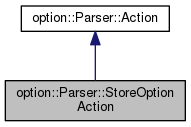
\includegraphics[width=215pt]{classoption_1_1Parser_1_1StoreOptionAction__inherit__graph}
\end{center}
\end{figure}


Collaboration diagram for option\+:\+:Parser\+:\+:Store\+Option\+Action\+:
\nopagebreak
\begin{figure}[H]
\begin{center}
\leavevmode
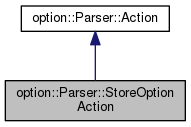
\includegraphics[width=215pt]{classoption_1_1Parser_1_1StoreOptionAction__coll__graph}
\end{center}
\end{figure}
\subsection*{Public Member Functions}
\begin{DoxyCompactItemize}
\item 
\hyperlink{classoption_1_1Parser_1_1StoreOptionAction_aaa638cdd712202e3e10471d4299f7f9d}{Store\+Option\+Action} (\hyperlink{classoption_1_1Parser}{Parser} \&parser\+\_\+, \hyperlink{classoption_1_1Option}{Option} options\+\_\+\mbox{[}$\,$\mbox{]}, \hyperlink{classoption_1_1Option}{Option} buffer\+\_\+\mbox{[}$\,$\mbox{]}, int bufmax\+\_\+)
\begin{DoxyCompactList}\small\item\em Number of slots in {\ttfamily buffer}. {\ttfamily -\/1} means \char`\"{}large enough\char`\"{}. \end{DoxyCompactList}\item 
bool \hyperlink{classoption_1_1Parser_1_1StoreOptionAction_a8931919fba5516377c202920db2b2f84}{perform} (\hyperlink{classoption_1_1Option}{Option} \&option)
\begin{DoxyCompactList}\small\item\em Called by Parser\+::workhorse() for each \hyperlink{classoption_1_1Option}{Option} that has been successfully parsed (including unknown options if they have a \hyperlink{structoption_1_1Descriptor}{Descriptor} whose \hyperlink{structoption_1_1Descriptor_aa5d675dba0214a4abd73007ff163cc67}{Descriptor\+::check\+\_\+arg} does not return \hyperlink{namespaceoption_aee8c76a07877335762631491e7a5a1a9a9528e32563b795bd2930b12d0a5e382d}{A\+R\+G\+\_\+\+I\+L\+L\+E\+G\+AL}. \end{DoxyCompactList}\item 
bool \hyperlink{classoption_1_1Parser_1_1StoreOptionAction_a617f675ef50a72ae36ce91f065bc8441}{finished} (int numargs, const char $\ast$$\ast$args)
\begin{DoxyCompactList}\small\item\em Called by Parser\+::workhorse() after finishing the parse. \end{DoxyCompactList}\end{DoxyCompactItemize}


\subsection{Constructor \& Destructor Documentation}
\index{option\+::\+Parser\+::\+Store\+Option\+Action@{option\+::\+Parser\+::\+Store\+Option\+Action}!Store\+Option\+Action@{Store\+Option\+Action}}
\index{Store\+Option\+Action@{Store\+Option\+Action}!option\+::\+Parser\+::\+Store\+Option\+Action@{option\+::\+Parser\+::\+Store\+Option\+Action}}
\subsubsection[{\texorpdfstring{Store\+Option\+Action(\+Parser \&parser\+\_\+, Option options\+\_\+[], Option buffer\+\_\+[], int bufmax\+\_\+)}{StoreOptionAction(Parser &parser_, Option options_[], Option buffer_[], int bufmax_)}}]{\setlength{\rightskip}{0pt plus 5cm}option\+::\+Parser\+::\+Store\+Option\+Action\+::\+Store\+Option\+Action (
\begin{DoxyParamCaption}
\item[{{\bf Parser} \&}]{parser\+\_\+, }
\item[{{\bf Option}}]{options\+\_\+\mbox{[}$\,$\mbox{]}, }
\item[{{\bf Option}}]{buffer\+\_\+\mbox{[}$\,$\mbox{]}, }
\item[{int}]{bufmax\+\_\+}
\end{DoxyParamCaption}
)\hspace{0.3cm}{\ttfamily [inline]}}\hypertarget{classoption_1_1Parser_1_1StoreOptionAction_aaa638cdd712202e3e10471d4299f7f9d}{}\label{classoption_1_1Parser_1_1StoreOptionAction_aaa638cdd712202e3e10471d4299f7f9d}


Number of slots in {\ttfamily buffer}. {\ttfamily -\/1} means \char`\"{}large enough\char`\"{}. 

Creates a new Store\+Option action. 
\begin{DoxyParams}{Parameters}
{\em parser\+\_\+} & the parser whose op\+\_\+count should be updated. \\
\hline
{\em options\+\_\+} & each \hyperlink{classoption_1_1Option}{Option} {\ttfamily o} is chained into the linked list {\ttfamily options\+\_\+}\mbox{[}o.\+desc-\/$>$index\mbox{]} \\
\hline
{\em buffer\+\_\+} & each \hyperlink{classoption_1_1Option}{Option} is appended to this array as long as there\textquotesingle{}s a free slot. \\
\hline
{\em bufmax\+\_\+} & number of slots in {\ttfamily buffer\+\_\+}. {\ttfamily -\/1} means \char`\"{}large enough\char`\"{}. \\
\hline
\end{DoxyParams}


\subsection{Member Function Documentation}
\index{option\+::\+Parser\+::\+Store\+Option\+Action@{option\+::\+Parser\+::\+Store\+Option\+Action}!finished@{finished}}
\index{finished@{finished}!option\+::\+Parser\+::\+Store\+Option\+Action@{option\+::\+Parser\+::\+Store\+Option\+Action}}
\subsubsection[{\texorpdfstring{finished(int numargs, const char $\ast$$\ast$args)}{finished(int numargs, const char **args)}}]{\setlength{\rightskip}{0pt plus 5cm}bool option\+::\+Parser\+::\+Store\+Option\+Action\+::finished (
\begin{DoxyParamCaption}
\item[{int}]{numargs, }
\item[{const char $\ast$$\ast$}]{args}
\end{DoxyParamCaption}
)\hspace{0.3cm}{\ttfamily [inline]}, {\ttfamily [virtual]}}\hypertarget{classoption_1_1Parser_1_1StoreOptionAction_a617f675ef50a72ae36ce91f065bc8441}{}\label{classoption_1_1Parser_1_1StoreOptionAction_a617f675ef50a72ae36ce91f065bc8441}


Called by Parser\+::workhorse() after finishing the parse. 


\begin{DoxyParams}{Parameters}
{\em numargs} & the number of non-\/option arguments remaining \\
\hline
{\em args} & pointer to the first remaining non-\/option argument (if numargs $>$ 0).\\
\hline
\end{DoxyParams}
\begin{DoxyReturn}{Returns}
{\ttfamily false} iff a fatal error has occurred. 
\end{DoxyReturn}


Reimplemented from \hyperlink{structoption_1_1Parser_1_1Action_a3ec558b51e34d33d116f14587289e032}{option\+::\+Parser\+::\+Action}.

\index{option\+::\+Parser\+::\+Store\+Option\+Action@{option\+::\+Parser\+::\+Store\+Option\+Action}!perform@{perform}}
\index{perform@{perform}!option\+::\+Parser\+::\+Store\+Option\+Action@{option\+::\+Parser\+::\+Store\+Option\+Action}}
\subsubsection[{\texorpdfstring{perform(\+Option \&option)}{perform(Option &option)}}]{\setlength{\rightskip}{0pt plus 5cm}bool option\+::\+Parser\+::\+Store\+Option\+Action\+::perform (
\begin{DoxyParamCaption}
\item[{{\bf Option} \&}]{}
\end{DoxyParamCaption}
)\hspace{0.3cm}{\ttfamily [inline]}, {\ttfamily [virtual]}}\hypertarget{classoption_1_1Parser_1_1StoreOptionAction_a8931919fba5516377c202920db2b2f84}{}\label{classoption_1_1Parser_1_1StoreOptionAction_a8931919fba5516377c202920db2b2f84}


Called by Parser\+::workhorse() for each \hyperlink{classoption_1_1Option}{Option} that has been successfully parsed (including unknown options if they have a \hyperlink{structoption_1_1Descriptor}{Descriptor} whose \hyperlink{structoption_1_1Descriptor_aa5d675dba0214a4abd73007ff163cc67}{Descriptor\+::check\+\_\+arg} does not return \hyperlink{namespaceoption_aee8c76a07877335762631491e7a5a1a9a9528e32563b795bd2930b12d0a5e382d}{A\+R\+G\+\_\+\+I\+L\+L\+E\+G\+AL}. 

Returns {\ttfamily false} iff a fatal error has occured and the parse should be aborted. 

Reimplemented from \hyperlink{structoption_1_1Parser_1_1Action_a176b5f783bb35eb015b6d2c09422457d}{option\+::\+Parser\+::\+Action}.



The documentation for this class was generated from the following file\+:\begin{DoxyCompactItemize}
\item 
\hyperlink{optionparser_8h}{optionparser.\+h}\end{DoxyCompactItemize}

\hypertarget{structoption_1_1PrintUsageImplementation_1_1StreamWriter}{}\section{option\+:\+:Print\+Usage\+Implementation\+:\+:Stream\+Writer$<$ Function, Stream $>$ Struct Template Reference}
\label{structoption_1_1PrintUsageImplementation_1_1StreamWriter}\index{option\+::\+Print\+Usage\+Implementation\+::\+Stream\+Writer$<$ Function, Stream $>$@{option\+::\+Print\+Usage\+Implementation\+::\+Stream\+Writer$<$ Function, Stream $>$}}


Inheritance diagram for option\+:\+:Print\+Usage\+Implementation\+:\+:Stream\+Writer$<$ Function, Stream $>$\+:
\nopagebreak
\begin{figure}[H]
\begin{center}
\leavevmode
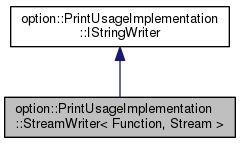
\includegraphics[width=253pt]{structoption_1_1PrintUsageImplementation_1_1StreamWriter__inherit__graph}
\end{center}
\end{figure}


Collaboration diagram for option\+:\+:Print\+Usage\+Implementation\+:\+:Stream\+Writer$<$ Function, Stream $>$\+:
\nopagebreak
\begin{figure}[H]
\begin{center}
\leavevmode
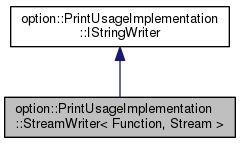
\includegraphics[width=253pt]{structoption_1_1PrintUsageImplementation_1_1StreamWriter__coll__graph}
\end{center}
\end{figure}
\subsection*{Public Member Functions}
\begin{DoxyCompactItemize}
\item 
virtual void \hyperlink{structoption_1_1PrintUsageImplementation_1_1StreamWriter_ae39bc6378c22d24a490104b7764c37b7}{operator()} (const char $\ast$str, int size)\hypertarget{structoption_1_1PrintUsageImplementation_1_1StreamWriter_ae39bc6378c22d24a490104b7764c37b7}{}\label{structoption_1_1PrintUsageImplementation_1_1StreamWriter_ae39bc6378c22d24a490104b7764c37b7}

\begin{DoxyCompactList}\small\item\em Writes the given number of chars beginning at the given pointer somewhere. \end{DoxyCompactList}\item 
{\bfseries Stream\+Writer} (Function $\ast$w, Stream $\ast$s)\hypertarget{structoption_1_1PrintUsageImplementation_1_1StreamWriter_aa6ab48848dcbeb9e2cbde5d05ec35005}{}\label{structoption_1_1PrintUsageImplementation_1_1StreamWriter_aa6ab48848dcbeb9e2cbde5d05ec35005}

\end{DoxyCompactItemize}
\subsection*{Public Attributes}
\begin{DoxyCompactItemize}
\item 
Function $\ast$ {\bfseries fwrite}\hypertarget{structoption_1_1PrintUsageImplementation_1_1StreamWriter_a6f54abc9a3f7f00206d87a3619713954}{}\label{structoption_1_1PrintUsageImplementation_1_1StreamWriter_a6f54abc9a3f7f00206d87a3619713954}

\item 
Stream $\ast$ {\bfseries stream}\hypertarget{structoption_1_1PrintUsageImplementation_1_1StreamWriter_ab4bfd31b1c37376505ccd4230f7f7ad9}{}\label{structoption_1_1PrintUsageImplementation_1_1StreamWriter_ab4bfd31b1c37376505ccd4230f7f7ad9}

\end{DoxyCompactItemize}


The documentation for this struct was generated from the following file\+:\begin{DoxyCompactItemize}
\item 
\hyperlink{optionparser_8h}{optionparser.\+h}\end{DoxyCompactItemize}

\hypertarget{classhebi_1_1Info_1_1StringField}{}\section{hebi\+:\+:Info\+:\+:String\+Field Class Reference}
\label{classhebi_1_1Info_1_1StringField}\index{hebi\+::\+Info\+::\+String\+Field@{hebi\+::\+Info\+::\+String\+Field}}


A message field representable by a std\+::string.  




{\ttfamily \#include $<$info.\+hpp$>$}

\subsection*{Public Member Functions}
\begin{DoxyCompactItemize}
\item 
{\bfseries String\+Field} (Hebi\+Info\+Ptr internal, Info\+String\+Field field)\hypertarget{classhebi_1_1Info_1_1StringField_a4a864517189aed3d613b6c55d92b6572}{}\label{classhebi_1_1Info_1_1StringField_a4a864517189aed3d613b6c55d92b6572}

\item 
\hyperlink{classhebi_1_1Info_1_1StringField_a04db0b8f4a982f083fd0ff4f5b49a6de}{operator bool} () const 
\begin{DoxyCompactList}\small\item\em Allows casting to a bool to check if the field has a value without directly calling {\ttfamily \hyperlink{classhebi_1_1Info_1_1StringField_aeb87dc356ac5284f12f461410151881f}{has()}}. \end{DoxyCompactList}\item 
bool \hyperlink{classhebi_1_1Info_1_1StringField_aeb87dc356ac5284f12f461410151881f}{has} () const \hypertarget{classhebi_1_1Info_1_1StringField_aeb87dc356ac5284f12f461410151881f}{}\label{classhebi_1_1Info_1_1StringField_aeb87dc356ac5284f12f461410151881f}

\begin{DoxyCompactList}\small\item\em True if (and only if) the field has a value. \end{DoxyCompactList}\item 
std\+::string \hyperlink{classhebi_1_1Info_1_1StringField_a6727fa4c435be34e94021ab87513e66a}{get} () const \hypertarget{classhebi_1_1Info_1_1StringField_a6727fa4c435be34e94021ab87513e66a}{}\label{classhebi_1_1Info_1_1StringField_a6727fa4c435be34e94021ab87513e66a}

\begin{DoxyCompactList}\small\item\em If the field has a value, returns a copy of that value; otherwise, returns a default. \end{DoxyCompactList}\end{DoxyCompactItemize}


\subsection{Detailed Description}
A message field representable by a std\+::string. 

\subsection{Member Function Documentation}
\index{hebi\+::\+Info\+::\+String\+Field@{hebi\+::\+Info\+::\+String\+Field}!operator bool@{operator bool}}
\index{operator bool@{operator bool}!hebi\+::\+Info\+::\+String\+Field@{hebi\+::\+Info\+::\+String\+Field}}
\subsubsection[{\texorpdfstring{operator bool() const }{operator bool() const }}]{\setlength{\rightskip}{0pt plus 5cm}hebi\+::\+Info\+::\+String\+Field\+::operator bool (
\begin{DoxyParamCaption}
{}
\end{DoxyParamCaption}
) const\hspace{0.3cm}{\ttfamily [explicit]}}\hypertarget{classhebi_1_1Info_1_1StringField_a04db0b8f4a982f083fd0ff4f5b49a6de}{}\label{classhebi_1_1Info_1_1StringField_a04db0b8f4a982f083fd0ff4f5b49a6de}


Allows casting to a bool to check if the field has a value without directly calling {\ttfamily \hyperlink{classhebi_1_1Info_1_1StringField_aeb87dc356ac5284f12f461410151881f}{has()}}. 

This can be used as in the following (assuming \textquotesingle{}parent\textquotesingle{} is a parent message, and this field is called \textquotesingle{}my\+Field\textquotesingle{}) 
\begin{DoxyCode}
Info::StringField& f = parent.myField();
\textcolor{keywordflow}{if} (f)
  std::cout << \textcolor{stringliteral}{"Field has value: "} << f.get() << std::endl;
\textcolor{keywordflow}{else}
  std::cout << \textcolor{stringliteral}{"Field has no value!"} << std::endl;
\end{DoxyCode}
 

The documentation for this class was generated from the following files\+:\begin{DoxyCompactItemize}
\item 
info.\+hpp\item 
info.\+cpp\end{DoxyCompactItemize}

\hypertarget{classhebi_1_1Command_1_1StringField}{}\section{hebi\+:\+:Command\+:\+:String\+Field Class Reference}
\label{classhebi_1_1Command_1_1StringField}\index{hebi\+::\+Command\+::\+String\+Field@{hebi\+::\+Command\+::\+String\+Field}}


A message field representable by a std\+::string.  




{\ttfamily \#include $<$command.\+hpp$>$}

\subsection*{Public Member Functions}
\begin{DoxyCompactItemize}
\item 
\mbox{\Hypertarget{classhebi_1_1Command_1_1StringField_ae7b2fffca27317a938a0915f1c184832}\label{classhebi_1_1Command_1_1StringField_ae7b2fffca27317a938a0915f1c184832}} 
{\bfseries String\+Field} (Hebi\+Command\+Ptr internal, Command\+String\+Field field)
\item 
\hyperlink{classhebi_1_1Command_1_1StringField_a6cb2fc39a5f13097c50dc89baf81aa61}{operator bool} () const
\begin{DoxyCompactList}\small\item\em Allows casting to a bool to check if the field has a value without directly calling {\ttfamily \hyperlink{classhebi_1_1Command_1_1StringField_ae05e05ab9e984b07f8ccc186b1d80833}{has()}}. \end{DoxyCompactList}\item 
\mbox{\Hypertarget{classhebi_1_1Command_1_1StringField_ae05e05ab9e984b07f8ccc186b1d80833}\label{classhebi_1_1Command_1_1StringField_ae05e05ab9e984b07f8ccc186b1d80833}} 
bool \hyperlink{classhebi_1_1Command_1_1StringField_ae05e05ab9e984b07f8ccc186b1d80833}{has} () const
\begin{DoxyCompactList}\small\item\em True if (and only if) the field has a value. \end{DoxyCompactList}\item 
\mbox{\Hypertarget{classhebi_1_1Command_1_1StringField_a0255f5ad404f37b46915941f98c5c8cd}\label{classhebi_1_1Command_1_1StringField_a0255f5ad404f37b46915941f98c5c8cd}} 
std\+::string \hyperlink{classhebi_1_1Command_1_1StringField_a0255f5ad404f37b46915941f98c5c8cd}{get} () const
\begin{DoxyCompactList}\small\item\em If the field has a value, returns a copy of that value; otherwise, returns a default. \end{DoxyCompactList}\item 
\mbox{\Hypertarget{classhebi_1_1Command_1_1StringField_aa5eb648c4d8d97fd8036abdaec0ec9e5}\label{classhebi_1_1Command_1_1StringField_aa5eb648c4d8d97fd8036abdaec0ec9e5}} 
void \hyperlink{classhebi_1_1Command_1_1StringField_aa5eb648c4d8d97fd8036abdaec0ec9e5}{set} (const std\+::string \&value)
\begin{DoxyCompactList}\small\item\em Sets the field to a given value. \end{DoxyCompactList}\item 
\mbox{\Hypertarget{classhebi_1_1Command_1_1StringField_aaae237fbd2d8a87b101f2687f91ccd0d}\label{classhebi_1_1Command_1_1StringField_aaae237fbd2d8a87b101f2687f91ccd0d}} 
void \hyperlink{classhebi_1_1Command_1_1StringField_aaae237fbd2d8a87b101f2687f91ccd0d}{clear} ()
\begin{DoxyCompactList}\small\item\em Removes any currently set value for this field. \end{DoxyCompactList}\end{DoxyCompactItemize}


\subsection{Detailed Description}
A message field representable by a std\+::string. 

\subsection{Member Function Documentation}
\mbox{\Hypertarget{classhebi_1_1Command_1_1StringField_a6cb2fc39a5f13097c50dc89baf81aa61}\label{classhebi_1_1Command_1_1StringField_a6cb2fc39a5f13097c50dc89baf81aa61}} 
\index{hebi\+::\+Command\+::\+String\+Field@{hebi\+::\+Command\+::\+String\+Field}!operator bool@{operator bool}}
\index{operator bool@{operator bool}!hebi\+::\+Command\+::\+String\+Field@{hebi\+::\+Command\+::\+String\+Field}}
\subsubsection{\texorpdfstring{operator bool()}{operator bool()}}
{\footnotesize\ttfamily hebi\+::\+Command\+::\+String\+Field\+::operator bool (\begin{DoxyParamCaption}{ }\end{DoxyParamCaption}) const\hspace{0.3cm}{\ttfamily [explicit]}}



Allows casting to a bool to check if the field has a value without directly calling {\ttfamily \hyperlink{classhebi_1_1Command_1_1StringField_ae05e05ab9e984b07f8ccc186b1d80833}{has()}}. 

This can be used as in the following (assuming \textquotesingle{}parent\textquotesingle{} is a parent message, and this field is called \textquotesingle{}my\+Field\textquotesingle{}) 
\begin{DoxyCode}
Command::StringField& f = parent.myField();
\textcolor{keywordflow}{if} (f)
  std::cout << \textcolor{stringliteral}{"Field has value: "} << f.get() << std::endl;
\textcolor{keywordflow}{else}
  std::cout << \textcolor{stringliteral}{"Field has no value!"} << std::endl;
\end{DoxyCode}
 

The documentation for this class was generated from the following files\+:\begin{DoxyCompactItemize}
\item 
command.\+hpp\item 
command.\+cpp\end{DoxyCompactItemize}

\hypertarget{structoption_1_1PrintUsageImplementation_1_1SyscallWriter}{}\section{option\+:\+:Print\+Usage\+Implementation\+:\+:Syscall\+Writer$<$ Syscall $>$ Struct Template Reference}
\label{structoption_1_1PrintUsageImplementation_1_1SyscallWriter}\index{option\+::\+Print\+Usage\+Implementation\+::\+Syscall\+Writer$<$ Syscall $>$@{option\+::\+Print\+Usage\+Implementation\+::\+Syscall\+Writer$<$ Syscall $>$}}


Inheritance diagram for option\+:\+:Print\+Usage\+Implementation\+:\+:Syscall\+Writer$<$ Syscall $>$\+:
\nopagebreak
\begin{figure}[H]
\begin{center}
\leavevmode
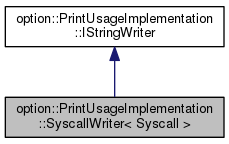
\includegraphics[width=244pt]{structoption_1_1PrintUsageImplementation_1_1SyscallWriter__inherit__graph}
\end{center}
\end{figure}


Collaboration diagram for option\+:\+:Print\+Usage\+Implementation\+:\+:Syscall\+Writer$<$ Syscall $>$\+:
\nopagebreak
\begin{figure}[H]
\begin{center}
\leavevmode
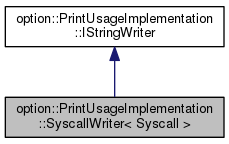
\includegraphics[width=244pt]{structoption_1_1PrintUsageImplementation_1_1SyscallWriter__coll__graph}
\end{center}
\end{figure}
\subsection*{Public Member Functions}
\begin{DoxyCompactItemize}
\item 
virtual void \hyperlink{structoption_1_1PrintUsageImplementation_1_1SyscallWriter_a61c1c010d9b67affd5f1208f0a3e9cf0}{operator()} (const char $\ast$str, int size)\hypertarget{structoption_1_1PrintUsageImplementation_1_1SyscallWriter_a61c1c010d9b67affd5f1208f0a3e9cf0}{}\label{structoption_1_1PrintUsageImplementation_1_1SyscallWriter_a61c1c010d9b67affd5f1208f0a3e9cf0}

\begin{DoxyCompactList}\small\item\em Writes the given number of chars beginning at the given pointer somewhere. \end{DoxyCompactList}\item 
{\bfseries Syscall\+Writer} (Syscall $\ast$w, int f)\hypertarget{structoption_1_1PrintUsageImplementation_1_1SyscallWriter_ae4f8677dbd79b0a9238368e28014701a}{}\label{structoption_1_1PrintUsageImplementation_1_1SyscallWriter_ae4f8677dbd79b0a9238368e28014701a}

\end{DoxyCompactItemize}
\subsection*{Public Attributes}
\begin{DoxyCompactItemize}
\item 
Syscall $\ast$ {\bfseries write}\hypertarget{structoption_1_1PrintUsageImplementation_1_1SyscallWriter_adc72b04cd74c69d0219b8b26589b8e5e}{}\label{structoption_1_1PrintUsageImplementation_1_1SyscallWriter_adc72b04cd74c69d0219b8b26589b8e5e}

\item 
int {\bfseries fd}\hypertarget{structoption_1_1PrintUsageImplementation_1_1SyscallWriter_ae79409e3f85f8dbaa7ef87bb8d7fcf8a}{}\label{structoption_1_1PrintUsageImplementation_1_1SyscallWriter_ae79409e3f85f8dbaa7ef87bb8d7fcf8a}

\end{DoxyCompactItemize}


The documentation for this struct was generated from the following file\+:\begin{DoxyCompactItemize}
\item 
\hyperlink{optionparser_8h}{optionparser.\+h}\end{DoxyCompactItemize}

\hypertarget{structoption_1_1PrintUsageImplementation_1_1TemporaryWriter}{}\section{option\+:\+:Print\+Usage\+Implementation\+:\+:Temporary\+Writer$<$ Temporary $>$ Struct Template Reference}
\label{structoption_1_1PrintUsageImplementation_1_1TemporaryWriter}\index{option\+::\+Print\+Usage\+Implementation\+::\+Temporary\+Writer$<$ Temporary $>$@{option\+::\+Print\+Usage\+Implementation\+::\+Temporary\+Writer$<$ Temporary $>$}}


Inheritance diagram for option\+:\+:Print\+Usage\+Implementation\+:\+:Temporary\+Writer$<$ Temporary $>$\+:\nopagebreak
\begin{figure}[H]
\begin{center}
\leavevmode
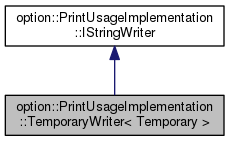
\includegraphics[width=244pt]{structoption_1_1PrintUsageImplementation_1_1TemporaryWriter__inherit__graph}
\end{center}
\end{figure}


Collaboration diagram for option\+:\+:Print\+Usage\+Implementation\+:\+:Temporary\+Writer$<$ Temporary $>$\+:\nopagebreak
\begin{figure}[H]
\begin{center}
\leavevmode
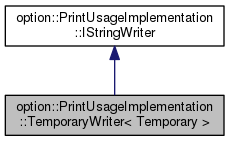
\includegraphics[width=244pt]{structoption_1_1PrintUsageImplementation_1_1TemporaryWriter__coll__graph}
\end{center}
\end{figure}
\subsection*{Public Member Functions}
\begin{DoxyCompactItemize}
\item 
virtual void \hyperlink{structoption_1_1PrintUsageImplementation_1_1TemporaryWriter_a674751ddfff63852b36c754878276b02}{operator()} (const char $\ast$str, int size)\hypertarget{structoption_1_1PrintUsageImplementation_1_1TemporaryWriter_a674751ddfff63852b36c754878276b02}{}\label{structoption_1_1PrintUsageImplementation_1_1TemporaryWriter_a674751ddfff63852b36c754878276b02}

\begin{DoxyCompactList}\small\item\em Writes the given number of chars beginning at the given pointer somewhere. \end{DoxyCompactList}\item 
{\bfseries Temporary\+Writer} (const Temporary \&u)\hypertarget{structoption_1_1PrintUsageImplementation_1_1TemporaryWriter_a0c65740b5a897ca2a2465d1c112882a8}{}\label{structoption_1_1PrintUsageImplementation_1_1TemporaryWriter_a0c65740b5a897ca2a2465d1c112882a8}

\end{DoxyCompactItemize}
\subsection*{Public Attributes}
\begin{DoxyCompactItemize}
\item 
const Temporary \& {\bfseries userstream}\hypertarget{structoption_1_1PrintUsageImplementation_1_1TemporaryWriter_a91d54cfcea7bb4072072506d46cc2cc8}{}\label{structoption_1_1PrintUsageImplementation_1_1TemporaryWriter_a91d54cfcea7bb4072072506d46cc2cc8}

\end{DoxyCompactItemize}


The documentation for this struct was generated from the following file\+:\begin{DoxyCompactItemize}
\item 
\hyperlink{optionparser_8h}{optionparser.\+h}\end{DoxyCompactItemize}

\hypertarget{classhebi_1_1Command_1_1Settings_1_1Actuator_1_1TorqueGains}{}\section{hebi\+:\+:Command\+:\+:Settings\+:\+:Actuator\+:\+:Torque\+Gains Class Reference}
\label{classhebi_1_1Command_1_1Settings_1_1Actuator_1_1TorqueGains}\index{hebi\+::\+Command\+::\+Settings\+::\+Actuator\+::\+Torque\+Gains@{hebi\+::\+Command\+::\+Settings\+::\+Actuator\+::\+Torque\+Gains}}


Controller gains for the torque P\+ID loop.  




{\ttfamily \#include $<$command.\+hpp$>$}

\subsection*{Public Member Functions}
\begin{DoxyCompactItemize}
\item 
\mbox{\Hypertarget{classhebi_1_1Command_1_1Settings_1_1Actuator_1_1TorqueGains_afa42dd5a96c691f833ad759c259bf114}\label{classhebi_1_1Command_1_1Settings_1_1Actuator_1_1TorqueGains_afa42dd5a96c691f833ad759c259bf114}} 
{\bfseries Torque\+Gains} (Hebi\+Command\+Ptr internal)
\item 
\mbox{\Hypertarget{classhebi_1_1Command_1_1Settings_1_1Actuator_1_1TorqueGains_a6c8edc2fb75a24ff07c2aba1b3dfd1d9}\label{classhebi_1_1Command_1_1Settings_1_1Actuator_1_1TorqueGains_a6c8edc2fb75a24ff07c2aba1b3dfd1d9}} 
\hyperlink{classhebi_1_1Command_1_1FloatField}{Float\+Field} \& \hyperlink{classhebi_1_1Command_1_1Settings_1_1Actuator_1_1TorqueGains_a6c8edc2fb75a24ff07c2aba1b3dfd1d9}{torque\+Kp} ()
\begin{DoxyCompactList}\small\item\em Proportional P\+ID gain for torque. \end{DoxyCompactList}\item 
\mbox{\Hypertarget{classhebi_1_1Command_1_1Settings_1_1Actuator_1_1TorqueGains_ab9318024d1c8de93282d62d1effb7d3f}\label{classhebi_1_1Command_1_1Settings_1_1Actuator_1_1TorqueGains_ab9318024d1c8de93282d62d1effb7d3f}} 
\hyperlink{classhebi_1_1Command_1_1FloatField}{Float\+Field} \& \hyperlink{classhebi_1_1Command_1_1Settings_1_1Actuator_1_1TorqueGains_ab9318024d1c8de93282d62d1effb7d3f}{torque\+Ki} ()
\begin{DoxyCompactList}\small\item\em Integral P\+ID gain for torque. \end{DoxyCompactList}\item 
\mbox{\Hypertarget{classhebi_1_1Command_1_1Settings_1_1Actuator_1_1TorqueGains_aa2dac4866009a37b306dd38d7c59c695}\label{classhebi_1_1Command_1_1Settings_1_1Actuator_1_1TorqueGains_aa2dac4866009a37b306dd38d7c59c695}} 
\hyperlink{classhebi_1_1Command_1_1FloatField}{Float\+Field} \& \hyperlink{classhebi_1_1Command_1_1Settings_1_1Actuator_1_1TorqueGains_aa2dac4866009a37b306dd38d7c59c695}{torque\+Kd} ()
\begin{DoxyCompactList}\small\item\em Derivative P\+ID gain for torque. \end{DoxyCompactList}\item 
\mbox{\Hypertarget{classhebi_1_1Command_1_1Settings_1_1Actuator_1_1TorqueGains_ab0e19d5a048f0190d73a1fb9fe9708da}\label{classhebi_1_1Command_1_1Settings_1_1Actuator_1_1TorqueGains_ab0e19d5a048f0190d73a1fb9fe9708da}} 
\hyperlink{classhebi_1_1Command_1_1FloatField}{Float\+Field} \& \hyperlink{classhebi_1_1Command_1_1Settings_1_1Actuator_1_1TorqueGains_ab0e19d5a048f0190d73a1fb9fe9708da}{torque\+Feed\+Forward} ()
\begin{DoxyCompactList}\small\item\em Feed forward term for torque (this term is multiplied by the target and added to the output). \end{DoxyCompactList}\item 
\mbox{\Hypertarget{classhebi_1_1Command_1_1Settings_1_1Actuator_1_1TorqueGains_af6a046c9f2382ecd14a175bda59e6dae}\label{classhebi_1_1Command_1_1Settings_1_1Actuator_1_1TorqueGains_af6a046c9f2382ecd14a175bda59e6dae}} 
\hyperlink{classhebi_1_1Command_1_1FloatField}{Float\+Field} \& \hyperlink{classhebi_1_1Command_1_1Settings_1_1Actuator_1_1TorqueGains_af6a046c9f2382ecd14a175bda59e6dae}{torque\+Dead\+Zone} ()
\begin{DoxyCompactList}\small\item\em Error values within +/-\/ this value from zero are treated as zero (in terms of computed proportional output, input to numerical derivative, and accumulated integral error). \end{DoxyCompactList}\item 
\mbox{\Hypertarget{classhebi_1_1Command_1_1Settings_1_1Actuator_1_1TorqueGains_ab9988770fc6d3d5132d6ee91671868a5}\label{classhebi_1_1Command_1_1Settings_1_1Actuator_1_1TorqueGains_ab9988770fc6d3d5132d6ee91671868a5}} 
\hyperlink{classhebi_1_1Command_1_1FloatField}{Float\+Field} \& \hyperlink{classhebi_1_1Command_1_1Settings_1_1Actuator_1_1TorqueGains_ab9988770fc6d3d5132d6ee91671868a5}{torque\+I\+Clamp} ()
\begin{DoxyCompactList}\small\item\em Maximum allowed value for the output of the integral component of the P\+ID loop; the integrated error is not allowed to exceed value that will generate this number. \end{DoxyCompactList}\item 
\mbox{\Hypertarget{classhebi_1_1Command_1_1Settings_1_1Actuator_1_1TorqueGains_a0a2c421d618aef63622cab0fc46d27e7}\label{classhebi_1_1Command_1_1Settings_1_1Actuator_1_1TorqueGains_a0a2c421d618aef63622cab0fc46d27e7}} 
\hyperlink{classhebi_1_1Command_1_1FloatField}{Float\+Field} \& \hyperlink{classhebi_1_1Command_1_1Settings_1_1Actuator_1_1TorqueGains_a0a2c421d618aef63622cab0fc46d27e7}{torque\+Punch} ()
\begin{DoxyCompactList}\small\item\em Constant offset to the torque P\+ID output outside of the deadzone; it is added when the error is positive and subtracted when it is negative. \end{DoxyCompactList}\item 
\mbox{\Hypertarget{classhebi_1_1Command_1_1Settings_1_1Actuator_1_1TorqueGains_a3de5880860ddd81711b241d62efa76f4}\label{classhebi_1_1Command_1_1Settings_1_1Actuator_1_1TorqueGains_a3de5880860ddd81711b241d62efa76f4}} 
\hyperlink{classhebi_1_1Command_1_1FloatField}{Float\+Field} \& \hyperlink{classhebi_1_1Command_1_1Settings_1_1Actuator_1_1TorqueGains_a3de5880860ddd81711b241d62efa76f4}{torque\+Min\+Target} ()
\begin{DoxyCompactList}\small\item\em Minimum allowed value for input to the P\+ID controller. \end{DoxyCompactList}\item 
\mbox{\Hypertarget{classhebi_1_1Command_1_1Settings_1_1Actuator_1_1TorqueGains_a28cffcd43a7f66008553806e9e15fbd2}\label{classhebi_1_1Command_1_1Settings_1_1Actuator_1_1TorqueGains_a28cffcd43a7f66008553806e9e15fbd2}} 
\hyperlink{classhebi_1_1Command_1_1FloatField}{Float\+Field} \& \hyperlink{classhebi_1_1Command_1_1Settings_1_1Actuator_1_1TorqueGains_a28cffcd43a7f66008553806e9e15fbd2}{torque\+Max\+Target} ()
\begin{DoxyCompactList}\small\item\em Maximum allowed value for input to the P\+ID controller. \end{DoxyCompactList}\item 
\mbox{\Hypertarget{classhebi_1_1Command_1_1Settings_1_1Actuator_1_1TorqueGains_aa6e4bb44277c15e41db428125c785de9}\label{classhebi_1_1Command_1_1Settings_1_1Actuator_1_1TorqueGains_aa6e4bb44277c15e41db428125c785de9}} 
\hyperlink{classhebi_1_1Command_1_1FloatField}{Float\+Field} \& \hyperlink{classhebi_1_1Command_1_1Settings_1_1Actuator_1_1TorqueGains_aa6e4bb44277c15e41db428125c785de9}{torque\+Target\+Lowpass} ()
\begin{DoxyCompactList}\small\item\em A simple lowpass filter applied to the target set point; needs to be between 0 and 1. At each timestep\+: x\+\_\+t = x\+\_\+t $\ast$ a + x\+\_\+\{t-\/1\} $\ast$ (1 -\/ a). \end{DoxyCompactList}\item 
\mbox{\Hypertarget{classhebi_1_1Command_1_1Settings_1_1Actuator_1_1TorqueGains_a22891ff90383ef13298ce8e059d7188a}\label{classhebi_1_1Command_1_1Settings_1_1Actuator_1_1TorqueGains_a22891ff90383ef13298ce8e059d7188a}} 
\hyperlink{classhebi_1_1Command_1_1FloatField}{Float\+Field} \& \hyperlink{classhebi_1_1Command_1_1Settings_1_1Actuator_1_1TorqueGains_a22891ff90383ef13298ce8e059d7188a}{torque\+Min\+Output} ()
\begin{DoxyCompactList}\small\item\em Output from the P\+ID controller is limited to a minimum of this value. \end{DoxyCompactList}\item 
\mbox{\Hypertarget{classhebi_1_1Command_1_1Settings_1_1Actuator_1_1TorqueGains_a590d35a63babac36bad9f6ab40572952}\label{classhebi_1_1Command_1_1Settings_1_1Actuator_1_1TorqueGains_a590d35a63babac36bad9f6ab40572952}} 
\hyperlink{classhebi_1_1Command_1_1FloatField}{Float\+Field} \& \hyperlink{classhebi_1_1Command_1_1Settings_1_1Actuator_1_1TorqueGains_a590d35a63babac36bad9f6ab40572952}{torque\+Max\+Output} ()
\begin{DoxyCompactList}\small\item\em Output from the P\+ID controller is limited to a maximum of this value. \end{DoxyCompactList}\item 
\mbox{\Hypertarget{classhebi_1_1Command_1_1Settings_1_1Actuator_1_1TorqueGains_a0920834b05619085b8fbd8b6b022333b}\label{classhebi_1_1Command_1_1Settings_1_1Actuator_1_1TorqueGains_a0920834b05619085b8fbd8b6b022333b}} 
\hyperlink{classhebi_1_1Command_1_1FloatField}{Float\+Field} \& \hyperlink{classhebi_1_1Command_1_1Settings_1_1Actuator_1_1TorqueGains_a0920834b05619085b8fbd8b6b022333b}{torque\+Output\+Lowpass} ()
\begin{DoxyCompactList}\small\item\em A simple lowpass filter applied to the controller output; needs to be between 0 and 1. At each timestep\+: x\+\_\+t = x\+\_\+t $\ast$ a + x\+\_\+\{t-\/1\} $\ast$ (1 -\/ a). \end{DoxyCompactList}\item 
\mbox{\Hypertarget{classhebi_1_1Command_1_1Settings_1_1Actuator_1_1TorqueGains_aeb0818f49f62f020c401a47930151b8c}\label{classhebi_1_1Command_1_1Settings_1_1Actuator_1_1TorqueGains_aeb0818f49f62f020c401a47930151b8c}} 
\hyperlink{classhebi_1_1Command_1_1BoolField}{Bool\+Field} \& \hyperlink{classhebi_1_1Command_1_1Settings_1_1Actuator_1_1TorqueGains_aeb0818f49f62f020c401a47930151b8c}{torque\+D\+On\+Error} ()
\begin{DoxyCompactList}\small\item\em Controls whether the Kd term uses the \char`\"{}derivative of error\char`\"{} or \char`\"{}derivative of measurement.\char`\"{} When the setpoints have step inputs or are noisy, setting this to {\ttfamily false} can eliminate corresponding spikes or noise in the output. \end{DoxyCompactList}\end{DoxyCompactItemize}


\subsection{Detailed Description}
Controller gains for the torque P\+ID loop. 

The documentation for this class was generated from the following file\+:\begin{DoxyCompactItemize}
\item 
command.\+hpp\end{DoxyCompactItemize}

\hypertarget{classhebi_1_1Info_1_1Settings_1_1Actuator_1_1TorqueGains}{}\section{hebi\+:\+:Info\+:\+:Settings\+:\+:Actuator\+:\+:Torque\+Gains Class Reference}
\label{classhebi_1_1Info_1_1Settings_1_1Actuator_1_1TorqueGains}\index{hebi\+::\+Info\+::\+Settings\+::\+Actuator\+::\+Torque\+Gains@{hebi\+::\+Info\+::\+Settings\+::\+Actuator\+::\+Torque\+Gains}}


Controller gains for the torque P\+ID loop.  




{\ttfamily \#include $<$info.\+hpp$>$}

\subsection*{Public Member Functions}
\begin{DoxyCompactItemize}
\item 
{\bfseries Torque\+Gains} (Hebi\+Info\+Ptr internal)\hypertarget{classhebi_1_1Info_1_1Settings_1_1Actuator_1_1TorqueGains_ad5639c348effdc06c2b03bd6bfd63023}{}\label{classhebi_1_1Info_1_1Settings_1_1Actuator_1_1TorqueGains_ad5639c348effdc06c2b03bd6bfd63023}

\item 
const \hyperlink{classhebi_1_1Info_1_1FloatField}{Float\+Field} \& \hyperlink{classhebi_1_1Info_1_1Settings_1_1Actuator_1_1TorqueGains_a3e308f454c57f98a0f9a2237adda20b3}{torque\+Kp} () const \hypertarget{classhebi_1_1Info_1_1Settings_1_1Actuator_1_1TorqueGains_a3e308f454c57f98a0f9a2237adda20b3}{}\label{classhebi_1_1Info_1_1Settings_1_1Actuator_1_1TorqueGains_a3e308f454c57f98a0f9a2237adda20b3}

\begin{DoxyCompactList}\small\item\em Proportional P\+ID gain for torque. \end{DoxyCompactList}\item 
const \hyperlink{classhebi_1_1Info_1_1FloatField}{Float\+Field} \& \hyperlink{classhebi_1_1Info_1_1Settings_1_1Actuator_1_1TorqueGains_a2a4ea1ab91ea376511e20c4923d76c89}{torque\+Ki} () const \hypertarget{classhebi_1_1Info_1_1Settings_1_1Actuator_1_1TorqueGains_a2a4ea1ab91ea376511e20c4923d76c89}{}\label{classhebi_1_1Info_1_1Settings_1_1Actuator_1_1TorqueGains_a2a4ea1ab91ea376511e20c4923d76c89}

\begin{DoxyCompactList}\small\item\em Integral P\+ID gain for torque. \end{DoxyCompactList}\item 
const \hyperlink{classhebi_1_1Info_1_1FloatField}{Float\+Field} \& \hyperlink{classhebi_1_1Info_1_1Settings_1_1Actuator_1_1TorqueGains_a8e782734a1835e93fb50e95be4d7fb97}{torque\+Kd} () const \hypertarget{classhebi_1_1Info_1_1Settings_1_1Actuator_1_1TorqueGains_a8e782734a1835e93fb50e95be4d7fb97}{}\label{classhebi_1_1Info_1_1Settings_1_1Actuator_1_1TorqueGains_a8e782734a1835e93fb50e95be4d7fb97}

\begin{DoxyCompactList}\small\item\em Derivative P\+ID gain for torque. \end{DoxyCompactList}\item 
const \hyperlink{classhebi_1_1Info_1_1FloatField}{Float\+Field} \& \hyperlink{classhebi_1_1Info_1_1Settings_1_1Actuator_1_1TorqueGains_a35f87e8b0513376a6584d6b2dcde631e}{torque\+Feed\+Forward} () const \hypertarget{classhebi_1_1Info_1_1Settings_1_1Actuator_1_1TorqueGains_a35f87e8b0513376a6584d6b2dcde631e}{}\label{classhebi_1_1Info_1_1Settings_1_1Actuator_1_1TorqueGains_a35f87e8b0513376a6584d6b2dcde631e}

\begin{DoxyCompactList}\small\item\em Feed forward term for torque (this term is multiplied by the target and added to the output). \end{DoxyCompactList}\item 
const \hyperlink{classhebi_1_1Info_1_1FloatField}{Float\+Field} \& \hyperlink{classhebi_1_1Info_1_1Settings_1_1Actuator_1_1TorqueGains_a2626b79437a08ccd5c1c5ac2aa8c3142}{torque\+Dead\+Zone} () const \hypertarget{classhebi_1_1Info_1_1Settings_1_1Actuator_1_1TorqueGains_a2626b79437a08ccd5c1c5ac2aa8c3142}{}\label{classhebi_1_1Info_1_1Settings_1_1Actuator_1_1TorqueGains_a2626b79437a08ccd5c1c5ac2aa8c3142}

\begin{DoxyCompactList}\small\item\em Error values within +/-\/ this value from zero are treated as zero (in terms of computed proportional output, input to numerical derivative, and accumulated integral error). \end{DoxyCompactList}\item 
const \hyperlink{classhebi_1_1Info_1_1FloatField}{Float\+Field} \& \hyperlink{classhebi_1_1Info_1_1Settings_1_1Actuator_1_1TorqueGains_ad7891144d29f8f64be2e34aa76c775b6}{torque\+I\+Clamp} () const \hypertarget{classhebi_1_1Info_1_1Settings_1_1Actuator_1_1TorqueGains_ad7891144d29f8f64be2e34aa76c775b6}{}\label{classhebi_1_1Info_1_1Settings_1_1Actuator_1_1TorqueGains_ad7891144d29f8f64be2e34aa76c775b6}

\begin{DoxyCompactList}\small\item\em Maximum allowed value for the output of the integral component of the P\+ID loop; the integrated error is not allowed to exceed value that will generate this number. \end{DoxyCompactList}\item 
const \hyperlink{classhebi_1_1Info_1_1FloatField}{Float\+Field} \& \hyperlink{classhebi_1_1Info_1_1Settings_1_1Actuator_1_1TorqueGains_a9fbb7aa71e799e48e4d2e1785309ef07}{torque\+Punch} () const \hypertarget{classhebi_1_1Info_1_1Settings_1_1Actuator_1_1TorqueGains_a9fbb7aa71e799e48e4d2e1785309ef07}{}\label{classhebi_1_1Info_1_1Settings_1_1Actuator_1_1TorqueGains_a9fbb7aa71e799e48e4d2e1785309ef07}

\begin{DoxyCompactList}\small\item\em Constant offset to the torque P\+ID output outside of the deadzone; it is added when the error is positive and subtracted when it is negative. \end{DoxyCompactList}\item 
const \hyperlink{classhebi_1_1Info_1_1FloatField}{Float\+Field} \& \hyperlink{classhebi_1_1Info_1_1Settings_1_1Actuator_1_1TorqueGains_a2b6f09420626f19f38e5ef9fc65788b6}{torque\+Min\+Target} () const \hypertarget{classhebi_1_1Info_1_1Settings_1_1Actuator_1_1TorqueGains_a2b6f09420626f19f38e5ef9fc65788b6}{}\label{classhebi_1_1Info_1_1Settings_1_1Actuator_1_1TorqueGains_a2b6f09420626f19f38e5ef9fc65788b6}

\begin{DoxyCompactList}\small\item\em Minimum allowed value for input to the P\+ID controller. \end{DoxyCompactList}\item 
const \hyperlink{classhebi_1_1Info_1_1FloatField}{Float\+Field} \& \hyperlink{classhebi_1_1Info_1_1Settings_1_1Actuator_1_1TorqueGains_acd6396cbd3f392d5fdde00f2de5c0d34}{torque\+Max\+Target} () const \hypertarget{classhebi_1_1Info_1_1Settings_1_1Actuator_1_1TorqueGains_acd6396cbd3f392d5fdde00f2de5c0d34}{}\label{classhebi_1_1Info_1_1Settings_1_1Actuator_1_1TorqueGains_acd6396cbd3f392d5fdde00f2de5c0d34}

\begin{DoxyCompactList}\small\item\em Maximum allowed value for input to the P\+ID controller. \end{DoxyCompactList}\item 
const \hyperlink{classhebi_1_1Info_1_1FloatField}{Float\+Field} \& \hyperlink{classhebi_1_1Info_1_1Settings_1_1Actuator_1_1TorqueGains_a9e8e121d824bd76280bad12affe62790}{torque\+Target\+Lowpass} () const \hypertarget{classhebi_1_1Info_1_1Settings_1_1Actuator_1_1TorqueGains_a9e8e121d824bd76280bad12affe62790}{}\label{classhebi_1_1Info_1_1Settings_1_1Actuator_1_1TorqueGains_a9e8e121d824bd76280bad12affe62790}

\begin{DoxyCompactList}\small\item\em A simple lowpass filter applied to the target set point; needs to be between 0 and 1. At each timestep\+: x\+\_\+t = x\+\_\+t $\ast$ a + x\+\_\+\{t-\/1\} $\ast$ (1 -\/ a). \end{DoxyCompactList}\item 
const \hyperlink{classhebi_1_1Info_1_1FloatField}{Float\+Field} \& \hyperlink{classhebi_1_1Info_1_1Settings_1_1Actuator_1_1TorqueGains_ace8cc45399ca1a56cd721816feee109b}{torque\+Min\+Output} () const \hypertarget{classhebi_1_1Info_1_1Settings_1_1Actuator_1_1TorqueGains_ace8cc45399ca1a56cd721816feee109b}{}\label{classhebi_1_1Info_1_1Settings_1_1Actuator_1_1TorqueGains_ace8cc45399ca1a56cd721816feee109b}

\begin{DoxyCompactList}\small\item\em Output from the P\+ID controller is limited to a minimum of this value. \end{DoxyCompactList}\item 
const \hyperlink{classhebi_1_1Info_1_1FloatField}{Float\+Field} \& \hyperlink{classhebi_1_1Info_1_1Settings_1_1Actuator_1_1TorqueGains_ab2decfb4905670824ecb423e1fcd89ea}{torque\+Max\+Output} () const \hypertarget{classhebi_1_1Info_1_1Settings_1_1Actuator_1_1TorqueGains_ab2decfb4905670824ecb423e1fcd89ea}{}\label{classhebi_1_1Info_1_1Settings_1_1Actuator_1_1TorqueGains_ab2decfb4905670824ecb423e1fcd89ea}

\begin{DoxyCompactList}\small\item\em Output from the P\+ID controller is limited to a maximum of this value. \end{DoxyCompactList}\item 
const \hyperlink{classhebi_1_1Info_1_1FloatField}{Float\+Field} \& \hyperlink{classhebi_1_1Info_1_1Settings_1_1Actuator_1_1TorqueGains_ad1d43336c922f567cbb8f1d2f5e1b159}{torque\+Output\+Lowpass} () const \hypertarget{classhebi_1_1Info_1_1Settings_1_1Actuator_1_1TorqueGains_ad1d43336c922f567cbb8f1d2f5e1b159}{}\label{classhebi_1_1Info_1_1Settings_1_1Actuator_1_1TorqueGains_ad1d43336c922f567cbb8f1d2f5e1b159}

\begin{DoxyCompactList}\small\item\em A simple lowpass filter applied to the controller output; needs to be between 0 and 1. At each timestep\+: x\+\_\+t = x\+\_\+t $\ast$ a + x\+\_\+\{t-\/1\} $\ast$ (1 -\/ a). \end{DoxyCompactList}\item 
const \hyperlink{classhebi_1_1Info_1_1BoolField}{Bool\+Field} \& \hyperlink{classhebi_1_1Info_1_1Settings_1_1Actuator_1_1TorqueGains_ac07e4b48f29d33e6b48590c482013d3a}{torque\+D\+On\+Error} () const \hypertarget{classhebi_1_1Info_1_1Settings_1_1Actuator_1_1TorqueGains_ac07e4b48f29d33e6b48590c482013d3a}{}\label{classhebi_1_1Info_1_1Settings_1_1Actuator_1_1TorqueGains_ac07e4b48f29d33e6b48590c482013d3a}

\begin{DoxyCompactList}\small\item\em Controls whether the Kd term uses the \char`\"{}derivative of error\char`\"{} or \char`\"{}derivative of measurement.\char`\"{} When the setpoints have step inputs or are noisy, setting this to {\ttfamily false} can eliminate corresponding spikes or noise in the output. \end{DoxyCompactList}\end{DoxyCompactItemize}


\subsection{Detailed Description}
Controller gains for the torque P\+ID loop. 

The documentation for this class was generated from the following file\+:\begin{DoxyCompactItemize}
\item 
info.\+hpp\end{DoxyCompactItemize}

\hypertarget{structhebi_1_1Vector3f}{}\section{hebi\+:\+:Vector3f Struct Reference}
\label{structhebi_1_1Vector3f}\index{hebi\+::\+Vector3f@{hebi\+::\+Vector3f}}


Structure to hold a 3-\/D floating point vector (i.\+e., x/y/z components)  




{\ttfamily \#include $<$vector\+\_\+3\+\_\+f.\+hpp$>$}

\subsection*{Public Member Functions}
\begin{DoxyCompactItemize}
\item 
\hyperlink{structhebi_1_1Vector3f_acde62a94c708091af51e133b76423505}{Vector3f} (float x, float y, float z)\hypertarget{structhebi_1_1Vector3f_acde62a94c708091af51e133b76423505}{}\label{structhebi_1_1Vector3f_acde62a94c708091af51e133b76423505}

\begin{DoxyCompactList}\small\item\em Create a 3-\/D floating point vector from three floating point components. \end{DoxyCompactList}\item 
\hyperlink{structhebi_1_1Vector3f_a7edaecafef5df6250ce2d72c3a9830d8}{Vector3f} (const Hebi\+Vector3f \&src)\hypertarget{structhebi_1_1Vector3f_a7edaecafef5df6250ce2d72c3a9830d8}{}\label{structhebi_1_1Vector3f_a7edaecafef5df6250ce2d72c3a9830d8}

\begin{DoxyCompactList}\small\item\em Method to create a C++ scoped \hyperlink{structhebi_1_1Vector3f}{hebi\+::\+Vector3f} object from an internal H\+E\+BI C A\+PI pointer. Internal use only. \end{DoxyCompactList}\item 
float \hyperlink{structhebi_1_1Vector3f_addc31da9b56506c51bd56e7f6db5deda}{getX} () const \hypertarget{structhebi_1_1Vector3f_addc31da9b56506c51bd56e7f6db5deda}{}\label{structhebi_1_1Vector3f_addc31da9b56506c51bd56e7f6db5deda}

\begin{DoxyCompactList}\small\item\em Returns the X component of the vector. \end{DoxyCompactList}\item 
float \hyperlink{structhebi_1_1Vector3f_a8564aa2ab2f815fa077a61d2705b1693}{getY} () const \hypertarget{structhebi_1_1Vector3f_a8564aa2ab2f815fa077a61d2705b1693}{}\label{structhebi_1_1Vector3f_a8564aa2ab2f815fa077a61d2705b1693}

\begin{DoxyCompactList}\small\item\em Returns the Y component of the vector. \end{DoxyCompactList}\item 
float \hyperlink{structhebi_1_1Vector3f_a1e507447c4b55d14b137aa50c8f0bbf3}{getZ} () const \hypertarget{structhebi_1_1Vector3f_a1e507447c4b55d14b137aa50c8f0bbf3}{}\label{structhebi_1_1Vector3f_a1e507447c4b55d14b137aa50c8f0bbf3}

\begin{DoxyCompactList}\small\item\em Returns the Z component of the vector. \end{DoxyCompactList}\end{DoxyCompactItemize}


\subsection{Detailed Description}
Structure to hold a 3-\/D floating point vector (i.\+e., x/y/z components) 

The documentation for this struct was generated from the following file\+:\begin{DoxyCompactItemize}
\item 
vector\+\_\+3\+\_\+f.\+hpp\end{DoxyCompactItemize}

\hypertarget{classhebi_1_1Feedback_1_1Vector3fField}{}\section{hebi\+:\+:Feedback\+:\+:Vector3f\+Field Class Reference}
\label{classhebi_1_1Feedback_1_1Vector3fField}\index{hebi\+::\+Feedback\+::\+Vector3f\+Field@{hebi\+::\+Feedback\+::\+Vector3f\+Field}}


A message field representable by a 3-\/D vector of single-\/precision floating point values.  




{\ttfamily \#include $<$feedback.\+hpp$>$}

\subsection*{Public Member Functions}
\begin{DoxyCompactItemize}
\item 
\mbox{\Hypertarget{classhebi_1_1Feedback_1_1Vector3fField_ab8f283eb2c0b88ddc08df740233a7d50}\label{classhebi_1_1Feedback_1_1Vector3fField_ab8f283eb2c0b88ddc08df740233a7d50}} 
{\bfseries Vector3f\+Field} (Hebi\+Feedback\+Ptr internal, Feedback\+Vector3f\+Field field)
\item 
\hyperlink{classhebi_1_1Feedback_1_1Vector3fField_a236d1c0aee3fea79769c9da36f1e1fbb}{operator bool} () const
\begin{DoxyCompactList}\small\item\em Allows casting to a bool to check if the field has a value without directly calling {\ttfamily \hyperlink{classhebi_1_1Feedback_1_1Vector3fField_a0484daa9aba07fe04f80467bf6501b0e}{has()}}. \end{DoxyCompactList}\item 
\mbox{\Hypertarget{classhebi_1_1Feedback_1_1Vector3fField_a0484daa9aba07fe04f80467bf6501b0e}\label{classhebi_1_1Feedback_1_1Vector3fField_a0484daa9aba07fe04f80467bf6501b0e}} 
bool \hyperlink{classhebi_1_1Feedback_1_1Vector3fField_a0484daa9aba07fe04f80467bf6501b0e}{has} () const
\begin{DoxyCompactList}\small\item\em True if (and only if) the field has a value. \end{DoxyCompactList}\item 
\mbox{\Hypertarget{classhebi_1_1Feedback_1_1Vector3fField_aca87a6c29cb168011bb81e18b30aa83e}\label{classhebi_1_1Feedback_1_1Vector3fField_aca87a6c29cb168011bb81e18b30aa83e}} 
\hyperlink{structhebi_1_1Vector3f}{Vector3f} \hyperlink{classhebi_1_1Feedback_1_1Vector3fField_aca87a6c29cb168011bb81e18b30aa83e}{get} () const
\begin{DoxyCompactList}\small\item\em If the field has a value, returns that value; otherwise, returns a default. \end{DoxyCompactList}\end{DoxyCompactItemize}


\subsection{Detailed Description}
A message field representable by a 3-\/D vector of single-\/precision floating point values. 

\subsection{Member Function Documentation}
\mbox{\Hypertarget{classhebi_1_1Feedback_1_1Vector3fField_a236d1c0aee3fea79769c9da36f1e1fbb}\label{classhebi_1_1Feedback_1_1Vector3fField_a236d1c0aee3fea79769c9da36f1e1fbb}} 
\index{hebi\+::\+Feedback\+::\+Vector3f\+Field@{hebi\+::\+Feedback\+::\+Vector3f\+Field}!operator bool@{operator bool}}
\index{operator bool@{operator bool}!hebi\+::\+Feedback\+::\+Vector3f\+Field@{hebi\+::\+Feedback\+::\+Vector3f\+Field}}
\subsubsection{\texorpdfstring{operator bool()}{operator bool()}}
{\footnotesize\ttfamily hebi\+::\+Feedback\+::\+Vector3f\+Field\+::operator bool (\begin{DoxyParamCaption}{ }\end{DoxyParamCaption}) const\hspace{0.3cm}{\ttfamily [explicit]}}



Allows casting to a bool to check if the field has a value without directly calling {\ttfamily \hyperlink{classhebi_1_1Feedback_1_1Vector3fField_a0484daa9aba07fe04f80467bf6501b0e}{has()}}. 

This can be used as in the following (assuming \textquotesingle{}parent\textquotesingle{} is a parent message, and this field is called \textquotesingle{}my\+Field\textquotesingle{}) 
\begin{DoxyCode}
Feedback::Vector3fField& f = parent.myField();
\textcolor{keywordflow}{if} (f)
  std::cout << \textcolor{stringliteral}{"Field has value!"} << std::endl;
\textcolor{keywordflow}{else}
  std::cout << \textcolor{stringliteral}{"Field has no value!"} << std::endl;
\end{DoxyCode}
 

The documentation for this class was generated from the following files\+:\begin{DoxyCompactItemize}
\item 
feedback.\+hpp\item 
feedback.\+cpp\end{DoxyCompactItemize}

\hypertarget{classhebi_1_1Info_1_1Settings_1_1Actuator_1_1VelocityGains}{}\section{hebi\+:\+:Info\+:\+:Settings\+:\+:Actuator\+:\+:Velocity\+Gains Class Reference}
\label{classhebi_1_1Info_1_1Settings_1_1Actuator_1_1VelocityGains}\index{hebi\+::\+Info\+::\+Settings\+::\+Actuator\+::\+Velocity\+Gains@{hebi\+::\+Info\+::\+Settings\+::\+Actuator\+::\+Velocity\+Gains}}


Controller gains for the velocity P\+ID loop.  




{\ttfamily \#include $<$info.\+hpp$>$}

\subsection*{Public Member Functions}
\begin{DoxyCompactItemize}
\item 
\mbox{\Hypertarget{classhebi_1_1Info_1_1Settings_1_1Actuator_1_1VelocityGains_a68d9acec8debedef74a338a6fd777911}\label{classhebi_1_1Info_1_1Settings_1_1Actuator_1_1VelocityGains_a68d9acec8debedef74a338a6fd777911}} 
{\bfseries Velocity\+Gains} (Hebi\+Info\+Ptr internal)
\item 
\mbox{\Hypertarget{classhebi_1_1Info_1_1Settings_1_1Actuator_1_1VelocityGains_a5cfe1ade10d5cfb147b854e6f885f61f}\label{classhebi_1_1Info_1_1Settings_1_1Actuator_1_1VelocityGains_a5cfe1ade10d5cfb147b854e6f885f61f}} 
const \hyperlink{classhebi_1_1Info_1_1FloatField}{Float\+Field} \& \hyperlink{classhebi_1_1Info_1_1Settings_1_1Actuator_1_1VelocityGains_a5cfe1ade10d5cfb147b854e6f885f61f}{velocity\+Kp} () const
\begin{DoxyCompactList}\small\item\em Proportional P\+ID gain for velocity. \end{DoxyCompactList}\item 
\mbox{\Hypertarget{classhebi_1_1Info_1_1Settings_1_1Actuator_1_1VelocityGains_a4f299a83826f1c6e0220034b735c8d5e}\label{classhebi_1_1Info_1_1Settings_1_1Actuator_1_1VelocityGains_a4f299a83826f1c6e0220034b735c8d5e}} 
const \hyperlink{classhebi_1_1Info_1_1FloatField}{Float\+Field} \& \hyperlink{classhebi_1_1Info_1_1Settings_1_1Actuator_1_1VelocityGains_a4f299a83826f1c6e0220034b735c8d5e}{velocity\+Ki} () const
\begin{DoxyCompactList}\small\item\em Integral P\+ID gain for velocity. \end{DoxyCompactList}\item 
\mbox{\Hypertarget{classhebi_1_1Info_1_1Settings_1_1Actuator_1_1VelocityGains_aa00887404607d040615e79d7e70c6676}\label{classhebi_1_1Info_1_1Settings_1_1Actuator_1_1VelocityGains_aa00887404607d040615e79d7e70c6676}} 
const \hyperlink{classhebi_1_1Info_1_1FloatField}{Float\+Field} \& \hyperlink{classhebi_1_1Info_1_1Settings_1_1Actuator_1_1VelocityGains_aa00887404607d040615e79d7e70c6676}{velocity\+Kd} () const
\begin{DoxyCompactList}\small\item\em Derivative P\+ID gain for velocity. \end{DoxyCompactList}\item 
\mbox{\Hypertarget{classhebi_1_1Info_1_1Settings_1_1Actuator_1_1VelocityGains_a3ab00f019709084fd6e79012c2f8fc54}\label{classhebi_1_1Info_1_1Settings_1_1Actuator_1_1VelocityGains_a3ab00f019709084fd6e79012c2f8fc54}} 
const \hyperlink{classhebi_1_1Info_1_1FloatField}{Float\+Field} \& \hyperlink{classhebi_1_1Info_1_1Settings_1_1Actuator_1_1VelocityGains_a3ab00f019709084fd6e79012c2f8fc54}{velocity\+Feed\+Forward} () const
\begin{DoxyCompactList}\small\item\em Feed forward term for velocity (this term is multiplied by the target and added to the output). \end{DoxyCompactList}\item 
\mbox{\Hypertarget{classhebi_1_1Info_1_1Settings_1_1Actuator_1_1VelocityGains_aadb1ec1ee69b354976d76b9bf232cfa2}\label{classhebi_1_1Info_1_1Settings_1_1Actuator_1_1VelocityGains_aadb1ec1ee69b354976d76b9bf232cfa2}} 
const \hyperlink{classhebi_1_1Info_1_1FloatField}{Float\+Field} \& \hyperlink{classhebi_1_1Info_1_1Settings_1_1Actuator_1_1VelocityGains_aadb1ec1ee69b354976d76b9bf232cfa2}{velocity\+Dead\+Zone} () const
\begin{DoxyCompactList}\small\item\em Error values within +/-\/ this value from zero are treated as zero (in terms of computed proportional output, input to numerical derivative, and accumulated integral error). \end{DoxyCompactList}\item 
\mbox{\Hypertarget{classhebi_1_1Info_1_1Settings_1_1Actuator_1_1VelocityGains_a88a73fe56df5290454cc930b9b348e6d}\label{classhebi_1_1Info_1_1Settings_1_1Actuator_1_1VelocityGains_a88a73fe56df5290454cc930b9b348e6d}} 
const \hyperlink{classhebi_1_1Info_1_1FloatField}{Float\+Field} \& \hyperlink{classhebi_1_1Info_1_1Settings_1_1Actuator_1_1VelocityGains_a88a73fe56df5290454cc930b9b348e6d}{velocity\+I\+Clamp} () const
\begin{DoxyCompactList}\small\item\em Maximum allowed value for the output of the integral component of the P\+ID loop; the integrated error is not allowed to exceed value that will generate this number. \end{DoxyCompactList}\item 
\mbox{\Hypertarget{classhebi_1_1Info_1_1Settings_1_1Actuator_1_1VelocityGains_a49be042463becdc3d166ad8c7c3a7194}\label{classhebi_1_1Info_1_1Settings_1_1Actuator_1_1VelocityGains_a49be042463becdc3d166ad8c7c3a7194}} 
const \hyperlink{classhebi_1_1Info_1_1FloatField}{Float\+Field} \& \hyperlink{classhebi_1_1Info_1_1Settings_1_1Actuator_1_1VelocityGains_a49be042463becdc3d166ad8c7c3a7194}{velocity\+Punch} () const
\begin{DoxyCompactList}\small\item\em Constant offset to the velocity P\+ID output outside of the deadzone; it is added when the error is positive and subtracted when it is negative. \end{DoxyCompactList}\item 
\mbox{\Hypertarget{classhebi_1_1Info_1_1Settings_1_1Actuator_1_1VelocityGains_a6901343fed9430b1874ce444fd415f2f}\label{classhebi_1_1Info_1_1Settings_1_1Actuator_1_1VelocityGains_a6901343fed9430b1874ce444fd415f2f}} 
const \hyperlink{classhebi_1_1Info_1_1FloatField}{Float\+Field} \& \hyperlink{classhebi_1_1Info_1_1Settings_1_1Actuator_1_1VelocityGains_a6901343fed9430b1874ce444fd415f2f}{velocity\+Min\+Target} () const
\begin{DoxyCompactList}\small\item\em Minimum allowed value for input to the P\+ID controller. \end{DoxyCompactList}\item 
\mbox{\Hypertarget{classhebi_1_1Info_1_1Settings_1_1Actuator_1_1VelocityGains_ab5aa7d4af03b7d995617d56e71c10369}\label{classhebi_1_1Info_1_1Settings_1_1Actuator_1_1VelocityGains_ab5aa7d4af03b7d995617d56e71c10369}} 
const \hyperlink{classhebi_1_1Info_1_1FloatField}{Float\+Field} \& \hyperlink{classhebi_1_1Info_1_1Settings_1_1Actuator_1_1VelocityGains_ab5aa7d4af03b7d995617d56e71c10369}{velocity\+Max\+Target} () const
\begin{DoxyCompactList}\small\item\em Maximum allowed value for input to the P\+ID controller. \end{DoxyCompactList}\item 
\mbox{\Hypertarget{classhebi_1_1Info_1_1Settings_1_1Actuator_1_1VelocityGains_aa5099bb7409c2f6e4d1cef72ca4275b2}\label{classhebi_1_1Info_1_1Settings_1_1Actuator_1_1VelocityGains_aa5099bb7409c2f6e4d1cef72ca4275b2}} 
const \hyperlink{classhebi_1_1Info_1_1FloatField}{Float\+Field} \& \hyperlink{classhebi_1_1Info_1_1Settings_1_1Actuator_1_1VelocityGains_aa5099bb7409c2f6e4d1cef72ca4275b2}{velocity\+Target\+Lowpass} () const
\begin{DoxyCompactList}\small\item\em A simple lowpass filter applied to the target set point; needs to be between 0 and 1. At each timestep\+: x\+\_\+t = x\+\_\+t $\ast$ a + x\+\_\+\{t-\/1\} $\ast$ (1 -\/ a). \end{DoxyCompactList}\item 
\mbox{\Hypertarget{classhebi_1_1Info_1_1Settings_1_1Actuator_1_1VelocityGains_a80501ce67ca67de1c8941827d315ab4d}\label{classhebi_1_1Info_1_1Settings_1_1Actuator_1_1VelocityGains_a80501ce67ca67de1c8941827d315ab4d}} 
const \hyperlink{classhebi_1_1Info_1_1FloatField}{Float\+Field} \& \hyperlink{classhebi_1_1Info_1_1Settings_1_1Actuator_1_1VelocityGains_a80501ce67ca67de1c8941827d315ab4d}{velocity\+Min\+Output} () const
\begin{DoxyCompactList}\small\item\em Output from the P\+ID controller is limited to a minimum of this value. \end{DoxyCompactList}\item 
\mbox{\Hypertarget{classhebi_1_1Info_1_1Settings_1_1Actuator_1_1VelocityGains_a7a3bc7815e6ca29d9ef6bce47383d44a}\label{classhebi_1_1Info_1_1Settings_1_1Actuator_1_1VelocityGains_a7a3bc7815e6ca29d9ef6bce47383d44a}} 
const \hyperlink{classhebi_1_1Info_1_1FloatField}{Float\+Field} \& \hyperlink{classhebi_1_1Info_1_1Settings_1_1Actuator_1_1VelocityGains_a7a3bc7815e6ca29d9ef6bce47383d44a}{velocity\+Max\+Output} () const
\begin{DoxyCompactList}\small\item\em Output from the P\+ID controller is limited to a maximum of this value. \end{DoxyCompactList}\item 
\mbox{\Hypertarget{classhebi_1_1Info_1_1Settings_1_1Actuator_1_1VelocityGains_a263735df9a41e39f820c5b88112e8427}\label{classhebi_1_1Info_1_1Settings_1_1Actuator_1_1VelocityGains_a263735df9a41e39f820c5b88112e8427}} 
const \hyperlink{classhebi_1_1Info_1_1FloatField}{Float\+Field} \& \hyperlink{classhebi_1_1Info_1_1Settings_1_1Actuator_1_1VelocityGains_a263735df9a41e39f820c5b88112e8427}{velocity\+Output\+Lowpass} () const
\begin{DoxyCompactList}\small\item\em A simple lowpass filter applied to the controller output; needs to be between 0 and 1. At each timestep\+: x\+\_\+t = x\+\_\+t $\ast$ a + x\+\_\+\{t-\/1\} $\ast$ (1 -\/ a). \end{DoxyCompactList}\item 
\mbox{\Hypertarget{classhebi_1_1Info_1_1Settings_1_1Actuator_1_1VelocityGains_ab448146439d8a6df5b55087495667b25}\label{classhebi_1_1Info_1_1Settings_1_1Actuator_1_1VelocityGains_ab448146439d8a6df5b55087495667b25}} 
const \hyperlink{classhebi_1_1Info_1_1BoolField}{Bool\+Field} \& \hyperlink{classhebi_1_1Info_1_1Settings_1_1Actuator_1_1VelocityGains_ab448146439d8a6df5b55087495667b25}{velocity\+D\+On\+Error} () const
\begin{DoxyCompactList}\small\item\em Controls whether the Kd term uses the \char`\"{}derivative of error\char`\"{} or \char`\"{}derivative of measurement.\char`\"{} When the setpoints have step inputs or are noisy, setting this to {\ttfamily false} can eliminate corresponding spikes or noise in the output. \end{DoxyCompactList}\end{DoxyCompactItemize}


\subsection{Detailed Description}
Controller gains for the velocity P\+ID loop. 

The documentation for this class was generated from the following file\+:\begin{DoxyCompactItemize}
\item 
info.\+hpp\end{DoxyCompactItemize}

\hypertarget{classhebi_1_1Command_1_1Settings_1_1Actuator_1_1VelocityGains}{}\section{hebi\+:\+:Command\+:\+:Settings\+:\+:Actuator\+:\+:Velocity\+Gains Class Reference}
\label{classhebi_1_1Command_1_1Settings_1_1Actuator_1_1VelocityGains}\index{hebi\+::\+Command\+::\+Settings\+::\+Actuator\+::\+Velocity\+Gains@{hebi\+::\+Command\+::\+Settings\+::\+Actuator\+::\+Velocity\+Gains}}


Controller gains for the velocity P\+ID loop.  




{\ttfamily \#include $<$command.\+hpp$>$}

\subsection*{Public Member Functions}
\begin{DoxyCompactItemize}
\item 
\mbox{\Hypertarget{classhebi_1_1Command_1_1Settings_1_1Actuator_1_1VelocityGains_afd7c86151a9c321ec1fb1f9c61bbae13}\label{classhebi_1_1Command_1_1Settings_1_1Actuator_1_1VelocityGains_afd7c86151a9c321ec1fb1f9c61bbae13}} 
{\bfseries Velocity\+Gains} (Hebi\+Command\+Ptr internal)
\item 
\mbox{\Hypertarget{classhebi_1_1Command_1_1Settings_1_1Actuator_1_1VelocityGains_a06f786482259f72e1c04928b831dc8f8}\label{classhebi_1_1Command_1_1Settings_1_1Actuator_1_1VelocityGains_a06f786482259f72e1c04928b831dc8f8}} 
\hyperlink{classhebi_1_1Command_1_1FloatField}{Float\+Field} \& \hyperlink{classhebi_1_1Command_1_1Settings_1_1Actuator_1_1VelocityGains_a06f786482259f72e1c04928b831dc8f8}{velocity\+Kp} ()
\begin{DoxyCompactList}\small\item\em Proportional P\+ID gain for velocity. \end{DoxyCompactList}\item 
\mbox{\Hypertarget{classhebi_1_1Command_1_1Settings_1_1Actuator_1_1VelocityGains_ab6d68b88b59e2bede320f3521fe4baa7}\label{classhebi_1_1Command_1_1Settings_1_1Actuator_1_1VelocityGains_ab6d68b88b59e2bede320f3521fe4baa7}} 
\hyperlink{classhebi_1_1Command_1_1FloatField}{Float\+Field} \& \hyperlink{classhebi_1_1Command_1_1Settings_1_1Actuator_1_1VelocityGains_ab6d68b88b59e2bede320f3521fe4baa7}{velocity\+Ki} ()
\begin{DoxyCompactList}\small\item\em Integral P\+ID gain for velocity. \end{DoxyCompactList}\item 
\mbox{\Hypertarget{classhebi_1_1Command_1_1Settings_1_1Actuator_1_1VelocityGains_aaa3e91ea679d6fb61b240b647e0b54d5}\label{classhebi_1_1Command_1_1Settings_1_1Actuator_1_1VelocityGains_aaa3e91ea679d6fb61b240b647e0b54d5}} 
\hyperlink{classhebi_1_1Command_1_1FloatField}{Float\+Field} \& \hyperlink{classhebi_1_1Command_1_1Settings_1_1Actuator_1_1VelocityGains_aaa3e91ea679d6fb61b240b647e0b54d5}{velocity\+Kd} ()
\begin{DoxyCompactList}\small\item\em Derivative P\+ID gain for velocity. \end{DoxyCompactList}\item 
\mbox{\Hypertarget{classhebi_1_1Command_1_1Settings_1_1Actuator_1_1VelocityGains_a4de848b17ddf892b1d474bac487dee3a}\label{classhebi_1_1Command_1_1Settings_1_1Actuator_1_1VelocityGains_a4de848b17ddf892b1d474bac487dee3a}} 
\hyperlink{classhebi_1_1Command_1_1FloatField}{Float\+Field} \& \hyperlink{classhebi_1_1Command_1_1Settings_1_1Actuator_1_1VelocityGains_a4de848b17ddf892b1d474bac487dee3a}{velocity\+Feed\+Forward} ()
\begin{DoxyCompactList}\small\item\em Feed forward term for velocity (this term is multiplied by the target and added to the output). \end{DoxyCompactList}\item 
\mbox{\Hypertarget{classhebi_1_1Command_1_1Settings_1_1Actuator_1_1VelocityGains_a2ea73387738ea5cbb084d8e50f077a7b}\label{classhebi_1_1Command_1_1Settings_1_1Actuator_1_1VelocityGains_a2ea73387738ea5cbb084d8e50f077a7b}} 
\hyperlink{classhebi_1_1Command_1_1FloatField}{Float\+Field} \& \hyperlink{classhebi_1_1Command_1_1Settings_1_1Actuator_1_1VelocityGains_a2ea73387738ea5cbb084d8e50f077a7b}{velocity\+Dead\+Zone} ()
\begin{DoxyCompactList}\small\item\em Error values within +/-\/ this value from zero are treated as zero (in terms of computed proportional output, input to numerical derivative, and accumulated integral error). \end{DoxyCompactList}\item 
\mbox{\Hypertarget{classhebi_1_1Command_1_1Settings_1_1Actuator_1_1VelocityGains_a2a5006c5ea06bfb46696c5afe1ebea03}\label{classhebi_1_1Command_1_1Settings_1_1Actuator_1_1VelocityGains_a2a5006c5ea06bfb46696c5afe1ebea03}} 
\hyperlink{classhebi_1_1Command_1_1FloatField}{Float\+Field} \& \hyperlink{classhebi_1_1Command_1_1Settings_1_1Actuator_1_1VelocityGains_a2a5006c5ea06bfb46696c5afe1ebea03}{velocity\+I\+Clamp} ()
\begin{DoxyCompactList}\small\item\em Maximum allowed value for the output of the integral component of the P\+ID loop; the integrated error is not allowed to exceed value that will generate this number. \end{DoxyCompactList}\item 
\mbox{\Hypertarget{classhebi_1_1Command_1_1Settings_1_1Actuator_1_1VelocityGains_a60aac6765a0d1679a57fd4c14ae96ed9}\label{classhebi_1_1Command_1_1Settings_1_1Actuator_1_1VelocityGains_a60aac6765a0d1679a57fd4c14ae96ed9}} 
\hyperlink{classhebi_1_1Command_1_1FloatField}{Float\+Field} \& \hyperlink{classhebi_1_1Command_1_1Settings_1_1Actuator_1_1VelocityGains_a60aac6765a0d1679a57fd4c14ae96ed9}{velocity\+Punch} ()
\begin{DoxyCompactList}\small\item\em Constant offset to the velocity P\+ID output outside of the deadzone; it is added when the error is positive and subtracted when it is negative. \end{DoxyCompactList}\item 
\mbox{\Hypertarget{classhebi_1_1Command_1_1Settings_1_1Actuator_1_1VelocityGains_a8e08b9592e6a33c54e35267b8fb1e2a2}\label{classhebi_1_1Command_1_1Settings_1_1Actuator_1_1VelocityGains_a8e08b9592e6a33c54e35267b8fb1e2a2}} 
\hyperlink{classhebi_1_1Command_1_1FloatField}{Float\+Field} \& \hyperlink{classhebi_1_1Command_1_1Settings_1_1Actuator_1_1VelocityGains_a8e08b9592e6a33c54e35267b8fb1e2a2}{velocity\+Min\+Target} ()
\begin{DoxyCompactList}\small\item\em Minimum allowed value for input to the P\+ID controller. \end{DoxyCompactList}\item 
\mbox{\Hypertarget{classhebi_1_1Command_1_1Settings_1_1Actuator_1_1VelocityGains_a96dc827b032b71be332c02499e0d334d}\label{classhebi_1_1Command_1_1Settings_1_1Actuator_1_1VelocityGains_a96dc827b032b71be332c02499e0d334d}} 
\hyperlink{classhebi_1_1Command_1_1FloatField}{Float\+Field} \& \hyperlink{classhebi_1_1Command_1_1Settings_1_1Actuator_1_1VelocityGains_a96dc827b032b71be332c02499e0d334d}{velocity\+Max\+Target} ()
\begin{DoxyCompactList}\small\item\em Maximum allowed value for input to the P\+ID controller. \end{DoxyCompactList}\item 
\mbox{\Hypertarget{classhebi_1_1Command_1_1Settings_1_1Actuator_1_1VelocityGains_a32c98ce7977d7e0751aa272691552dae}\label{classhebi_1_1Command_1_1Settings_1_1Actuator_1_1VelocityGains_a32c98ce7977d7e0751aa272691552dae}} 
\hyperlink{classhebi_1_1Command_1_1FloatField}{Float\+Field} \& \hyperlink{classhebi_1_1Command_1_1Settings_1_1Actuator_1_1VelocityGains_a32c98ce7977d7e0751aa272691552dae}{velocity\+Target\+Lowpass} ()
\begin{DoxyCompactList}\small\item\em A simple lowpass filter applied to the target set point; needs to be between 0 and 1. At each timestep\+: x\+\_\+t = x\+\_\+t $\ast$ a + x\+\_\+\{t-\/1\} $\ast$ (1 -\/ a). \end{DoxyCompactList}\item 
\mbox{\Hypertarget{classhebi_1_1Command_1_1Settings_1_1Actuator_1_1VelocityGains_aebc8db25cd3cb2756415953cf0d0a507}\label{classhebi_1_1Command_1_1Settings_1_1Actuator_1_1VelocityGains_aebc8db25cd3cb2756415953cf0d0a507}} 
\hyperlink{classhebi_1_1Command_1_1FloatField}{Float\+Field} \& \hyperlink{classhebi_1_1Command_1_1Settings_1_1Actuator_1_1VelocityGains_aebc8db25cd3cb2756415953cf0d0a507}{velocity\+Min\+Output} ()
\begin{DoxyCompactList}\small\item\em Output from the P\+ID controller is limited to a minimum of this value. \end{DoxyCompactList}\item 
\mbox{\Hypertarget{classhebi_1_1Command_1_1Settings_1_1Actuator_1_1VelocityGains_a98c49a0a9f30665f3853ba5fb40ab0e3}\label{classhebi_1_1Command_1_1Settings_1_1Actuator_1_1VelocityGains_a98c49a0a9f30665f3853ba5fb40ab0e3}} 
\hyperlink{classhebi_1_1Command_1_1FloatField}{Float\+Field} \& \hyperlink{classhebi_1_1Command_1_1Settings_1_1Actuator_1_1VelocityGains_a98c49a0a9f30665f3853ba5fb40ab0e3}{velocity\+Max\+Output} ()
\begin{DoxyCompactList}\small\item\em Output from the P\+ID controller is limited to a maximum of this value. \end{DoxyCompactList}\item 
\mbox{\Hypertarget{classhebi_1_1Command_1_1Settings_1_1Actuator_1_1VelocityGains_af9258452e76fad7bbd0249b5f8567d02}\label{classhebi_1_1Command_1_1Settings_1_1Actuator_1_1VelocityGains_af9258452e76fad7bbd0249b5f8567d02}} 
\hyperlink{classhebi_1_1Command_1_1FloatField}{Float\+Field} \& \hyperlink{classhebi_1_1Command_1_1Settings_1_1Actuator_1_1VelocityGains_af9258452e76fad7bbd0249b5f8567d02}{velocity\+Output\+Lowpass} ()
\begin{DoxyCompactList}\small\item\em A simple lowpass filter applied to the controller output; needs to be between 0 and 1. At each timestep\+: x\+\_\+t = x\+\_\+t $\ast$ a + x\+\_\+\{t-\/1\} $\ast$ (1 -\/ a). \end{DoxyCompactList}\item 
\mbox{\Hypertarget{classhebi_1_1Command_1_1Settings_1_1Actuator_1_1VelocityGains_a986a2c7629468de54443dfb4a77a6fb2}\label{classhebi_1_1Command_1_1Settings_1_1Actuator_1_1VelocityGains_a986a2c7629468de54443dfb4a77a6fb2}} 
\hyperlink{classhebi_1_1Command_1_1BoolField}{Bool\+Field} \& \hyperlink{classhebi_1_1Command_1_1Settings_1_1Actuator_1_1VelocityGains_a986a2c7629468de54443dfb4a77a6fb2}{velocity\+D\+On\+Error} ()
\begin{DoxyCompactList}\small\item\em Controls whether the Kd term uses the \char`\"{}derivative of error\char`\"{} or \char`\"{}derivative of measurement.\char`\"{} When the setpoints have step inputs or are noisy, setting this to {\ttfamily false} can eliminate corresponding spikes or noise in the output. \end{DoxyCompactList}\end{DoxyCompactItemize}


\subsection{Detailed Description}
Controller gains for the velocity P\+ID loop. 

The documentation for this class was generated from the following file\+:\begin{DoxyCompactItemize}
\item 
command.\+hpp\end{DoxyCompactItemize}

\chapter{File Documentation}
\hypertarget{lookup__helpers_8cpp}{}\section{lookup\+\_\+helpers.\+cpp File Reference}
\label{lookup__helpers_8cpp}\index{lookup\+\_\+helpers.\+cpp@{lookup\+\_\+helpers.\+cpp}}
{\ttfamily \#include \char`\"{}lookup.\+hpp\char`\"{}}\\*
{\ttfamily \#include \char`\"{}module.\+hpp\char`\"{}}\\*
{\ttfamily \#include \char`\"{}group.\+hpp\char`\"{}}\\*
{\ttfamily \#include \char`\"{}mac\+\_\+address.\+hpp\char`\"{}}\\*
{\ttfamily \#include \char`\"{}optionparser.\+h\char`\"{}}\\*
{\ttfamily \#include $<$iostream$>$}\\*
Include dependency graph for lookup\+\_\+helpers.\+cpp\+:\nopagebreak
\begin{figure}[H]
\begin{center}
\leavevmode
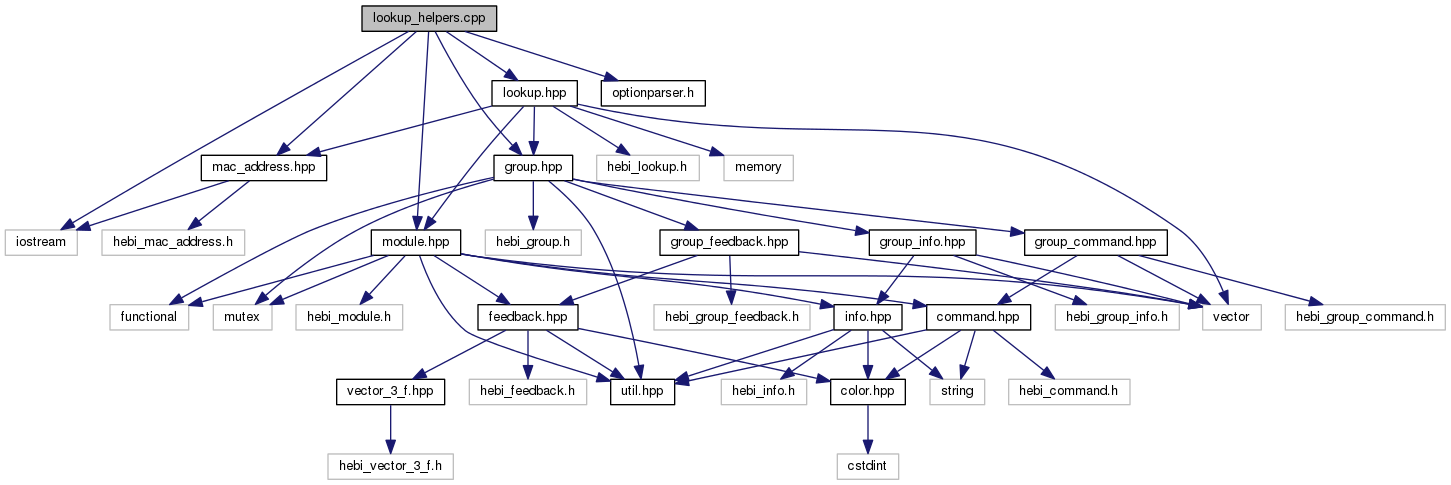
\includegraphics[width=350pt]{lookup__helpers_8cpp__incl}
\end{center}
\end{figure}
\subsection*{Classes}
\begin{DoxyCompactItemize}
\item 
struct \hyperlink{structArg}{Arg}
\end{DoxyCompactItemize}
\subsection*{Enumerations}
\begin{DoxyCompactItemize}
\item 
enum {\bfseries option\+Index} \{ \\*
{\bfseries U\+N\+K\+N\+O\+WN}, 
{\bfseries H\+E\+LP}, 
{\bfseries V\+E\+R\+B\+O\+SE}, 
{\bfseries N\+A\+ME}, 
\\*
{\bfseries F\+A\+M\+I\+LY}, 
{\bfseries P\+A\+IR}, 
{\bfseries M\+AC}, 
{\bfseries N\+A\+M\+ES}, 
\\*
{\bfseries F\+A\+M\+I\+L\+I\+ES}, 
{\bfseries P\+A\+I\+RS}, 
{\bfseries M\+A\+CS}
 \}\hypertarget{lookup__helpers_8cpp_a0ba79095c558cb72ea2e8b277be1da39}{}\label{lookup__helpers_8cpp_a0ba79095c558cb72ea2e8b277be1da39}

\end{DoxyCompactItemize}
\subsection*{Functions}
\begin{DoxyCompactItemize}
\item 
std\+::unique\+\_\+ptr$<$ \hyperlink{classhebi_1_1Module}{hebi\+::\+Module} $>$ \hyperlink{lookup__helpers_8cpp_a4eaf3947ef42501a94b2c32913176f57}{get\+Module\+From\+Args} (int argc, char $\ast$argv\mbox{[}$\,$\mbox{]})
\item 
std\+::unique\+\_\+ptr$<$ \hyperlink{classhebi_1_1Group}{hebi\+::\+Group} $>$ \hyperlink{lookup__helpers_8cpp_a6db32406bd0d0eac1eebcf2fd261af8e}{get\+Group\+From\+Args} (int argc, char $\ast$argv\mbox{[}$\,$\mbox{]})
\end{DoxyCompactItemize}
\subsection*{Variables}
\begin{DoxyCompactItemize}
\item 
const \hyperlink{structoption_1_1Descriptor}{option\+::\+Descriptor} {\bfseries module\+Usage} \mbox{[}$\,$\mbox{]}
\item 
const \hyperlink{structoption_1_1Descriptor}{option\+::\+Descriptor} {\bfseries group\+Usage} \mbox{[}$\,$\mbox{]}
\end{DoxyCompactItemize}


\subsection{Detailed Description}
common helper functions used by various examples.

\begin{DoxyAuthor}{Author}
Matthew Tesch $<$ matt @ hebirobotics.\+com $>$ 
\end{DoxyAuthor}
\begin{DoxySince}{Since}
22 Jan 2016 
\end{DoxySince}


\subsection{Function Documentation}
\index{lookup\+\_\+helpers.\+cpp@{lookup\+\_\+helpers.\+cpp}!get\+Group\+From\+Args@{get\+Group\+From\+Args}}
\index{get\+Group\+From\+Args@{get\+Group\+From\+Args}!lookup\+\_\+helpers.\+cpp@{lookup\+\_\+helpers.\+cpp}}
\subsubsection[{\texorpdfstring{get\+Group\+From\+Args(int argc, char $\ast$argv[])}{getGroupFromArgs(int argc, char *argv[])}}]{\setlength{\rightskip}{0pt plus 5cm}std\+::unique\+\_\+ptr$<${\bf hebi\+::\+Group}$>$ get\+Group\+From\+Args (
\begin{DoxyParamCaption}
\item[{int}]{argc, }
\item[{char $\ast$}]{argv\mbox{[}$\,$\mbox{]}}
\end{DoxyParamCaption}
)}\hypertarget{lookup__helpers_8cpp_a6db32406bd0d0eac1eebcf2fd261af8e}{}\label{lookup__helpers_8cpp_a6db32406bd0d0eac1eebcf2fd261af8e}
Parse the given arguments, and look up group based on the given arguments.

\begin{DoxyAuthor}{Author}
Matthew Tesch $<$ matt @ hebirobotics.\+com $>$ 
\end{DoxyAuthor}
\begin{DoxySince}{Since}
22 Jan 2016 
\end{DoxySince}
\index{lookup\+\_\+helpers.\+cpp@{lookup\+\_\+helpers.\+cpp}!get\+Module\+From\+Args@{get\+Module\+From\+Args}}
\index{get\+Module\+From\+Args@{get\+Module\+From\+Args}!lookup\+\_\+helpers.\+cpp@{lookup\+\_\+helpers.\+cpp}}
\subsubsection[{\texorpdfstring{get\+Module\+From\+Args(int argc, char $\ast$argv[])}{getModuleFromArgs(int argc, char *argv[])}}]{\setlength{\rightskip}{0pt plus 5cm}std\+::unique\+\_\+ptr$<${\bf hebi\+::\+Module}$>$ get\+Module\+From\+Args (
\begin{DoxyParamCaption}
\item[{int}]{argc, }
\item[{char $\ast$}]{argv\mbox{[}$\,$\mbox{]}}
\end{DoxyParamCaption}
)}\hypertarget{lookup__helpers_8cpp_a4eaf3947ef42501a94b2c32913176f57}{}\label{lookup__helpers_8cpp_a4eaf3947ef42501a94b2c32913176f57}
Parse the given arguments, and look up module based on the given arguments.

\begin{DoxyAuthor}{Author}
Matthew Tesch $<$ matt @ hebirobotics.\+com $>$ 
\end{DoxyAuthor}
\begin{DoxySince}{Since}
22 May 2016 
\end{DoxySince}


\subsection{Variable Documentation}
\index{lookup\+\_\+helpers.\+cpp@{lookup\+\_\+helpers.\+cpp}!group\+Usage@{group\+Usage}}
\index{group\+Usage@{group\+Usage}!lookup\+\_\+helpers.\+cpp@{lookup\+\_\+helpers.\+cpp}}
\subsubsection[{\texorpdfstring{group\+Usage}{groupUsage}}]{\setlength{\rightskip}{0pt plus 5cm}const {\bf option\+::\+Descriptor} group\+Usage\mbox{[}$\,$\mbox{]}}\hypertarget{lookup__helpers_8cpp_a801705ccfc80f1cad2bc748bc7367755}{}\label{lookup__helpers_8cpp_a801705ccfc80f1cad2bc748bc7367755}
{\bfseries Initial value\+:}
\begin{DoxyCode}
=
\{
  \{ UNKNOWN, 0, \textcolor{stringliteral}{""}, \textcolor{stringliteral}{""},            Arg::Unknown, \textcolor{stringliteral}{"USAGE: program\_name [options]\(\backslash\)n\(\backslash\)n"}
    \textcolor{stringliteral}{"Options are parsed to determine search terms for group. User can either provide:\(\backslash\)n"}
    \textcolor{stringliteral}{" 1) single module specification to form connected group (-p, -n/-f, or -m)\(\backslash\)n"}
    \textcolor{stringliteral}{" 2) list of families and list of names independently (-F and -N)\(\backslash\)n"}
    \textcolor{stringliteral}{" 3) list of family/name pairs (-P)\(\backslash\)n"}
    \textcolor{stringliteral}{" 4) list of mac addresses (-M)\(\backslash\)n\(\backslash\)n"}
    \textcolor{stringliteral}{"Options:"} \},
  \{ HELP,    0, \textcolor{stringliteral}{"h"}, \textcolor{stringliteral}{"help"},       \hyperlink{structoption_1_1Arg_a7fc01987899c91c6b6a1be5711a46e22}{option::Arg::None}, \textcolor{stringliteral}{"  -h, \(\backslash\)t--help  \(\backslash\)tPrint this help
       and exit."} \},
  \{ VERBOSE, 0, \textcolor{stringliteral}{"v"}, \textcolor{stringliteral}{"verbose"},    \hyperlink{structoption_1_1Arg_a7fc01987899c91c6b6a1be5711a46e22}{option::Arg::None}, \textcolor{stringliteral}{"  -v, \(\backslash\)t--verbose  \(\backslash\)tVerbose output
       is enabled to help diagnose lookup issues."} \},
  \{ NAME,    0, \textcolor{stringliteral}{"n"}, \textcolor{stringliteral}{"name"},       Arg::NonEmpty, \textcolor{stringliteral}{"  -n <name>, \(\backslash\)t--name=<name> \(\backslash\)tName of the module; only
       for use in combination with '-f'. Used to create a group from all connected modules."} \},
  \{ FAMILY,  0, \textcolor{stringliteral}{"f"}, \textcolor{stringliteral}{"family"},     Arg::NonEmpty, \textcolor{stringliteral}{"  -f <family\_name>, \(\backslash\)t--family=<family\_name> \(\backslash\)tName of
       the family; only for use in combination with '-n'. Used to create a group from all connected modules."} \},
  \{ PAIR,    0, \textcolor{stringliteral}{"p"}, \textcolor{stringliteral}{"pair"},       Arg::Pair, \textcolor{stringliteral}{"  -p <name pair>, \(\backslash\)t--pair=<name pair> \(\backslash\)tFamily + name pair;
       must write as family\_name|name, with '|' symbol between family and name.  (Note: may need to escape the '|'
       character in some shells). Creates a group from all connected modules."} \},
  \{ MAC,     0, \textcolor{stringliteral}{"m"}, \textcolor{stringliteral}{"mac"},        Arg::Mac, \textcolor{stringliteral}{"  -m <mac>, \(\backslash\)t--mac=<mac> \(\backslash\)tMAC address of the module; must
       be given in following format: 01:23:45:ab:cd:ef.  Creates a group from all connected modules."} \},
  \{ NAMES,    0, \textcolor{stringliteral}{"N"}, \textcolor{stringliteral}{"names"},       Arg::NonEmpty, \textcolor{stringliteral}{"  -N <name> \(\backslash\)t--names=<name> \(\backslash\)tUsed to define a set of
       module names; each '-N' or '--names' argument is another module.  Only for use in combination with '-F'."} \}
      ,
  \{ FAMILIES,  0, \textcolor{stringliteral}{"F"}, \textcolor{stringliteral}{"families"},     Arg::NonEmpty, \textcolor{stringliteral}{"  -F <family\_name>, \(\backslash\)t--families=<family\_name> \(\backslash\)t
      Used to define a set of family names; each '-F' or '--families' argument is another family. Only for use in
       combination with '-N'. Each -F/--families argument is combined pairwise with each -N/--names argument.  If only
       one '-F' is given for a list of '-N' arguments, it applies to each '-N'."} \},
  \{ PAIRS,    0, \textcolor{stringliteral}{"P"}, \textcolor{stringliteral}{"pairs"},       Arg::Pair, \textcolor{stringliteral}{"  -P <name pair>, \(\backslash\)t--pairs=<name pair> \(\backslash\)tUsed to define a
       set of family + name pairs; each '-P' or '--pairs' argument is another pair. Matches format of '-p'
       argument."} \},
  \{ MACS,     0, \textcolor{stringliteral}{"M"}, \textcolor{stringliteral}{"macs"},        Arg::Mac, \textcolor{stringliteral}{"  -M <mac>, \(\backslash\)t--macs=<mac> \(\backslash\)tUsed to define a set of MAC
       addresses; each '-M' argument is another mac address. Matches format of '-m' argument."} \},
  \{ UNKNOWN, 0, \textcolor{stringliteral}{""}, \textcolor{stringliteral}{""}, \hyperlink{structoption_1_1Arg_a7fc01987899c91c6b6a1be5711a46e22}{option::Arg::None},
 \textcolor{stringliteral}{"\(\backslash\)nExamples:\(\backslash\)n"}
 \textcolor{stringliteral}{"  ./script -nModule05 -fArm \(\backslash\)n"}
 \textcolor{stringliteral}{"  ./script -pArm|Module05 \(\backslash\)n"}
 \textcolor{stringliteral}{"  ./script -ma1:2f:45:a3:c9:ef \(\backslash\)n"}
 \textcolor{stringliteral}{"  ./script -NModule05 -NModule07 -NModule02 -FArm -FArm -FArm \(\backslash\)n"}
 \textcolor{stringliteral}{"  ./script -N Module05 -N Module07 -N Module02 -F Arm \(\backslash\)n"}
 \textcolor{stringliteral}{"  ./script -P Arm|Module05 -P Arm|Module06 \(\backslash\)n"}
 \textcolor{stringliteral}{"  ./script -M 01:ab:23:4b:cd:4f --macs 0f:a4:25:a4:fe:3d \(\backslash\)n"} \},
\{ 0, 0, 0, 0, 0, 0 \} \}
\end{DoxyCode}
\index{lookup\+\_\+helpers.\+cpp@{lookup\+\_\+helpers.\+cpp}!module\+Usage@{module\+Usage}}
\index{module\+Usage@{module\+Usage}!lookup\+\_\+helpers.\+cpp@{lookup\+\_\+helpers.\+cpp}}
\subsubsection[{\texorpdfstring{module\+Usage}{moduleUsage}}]{\setlength{\rightskip}{0pt plus 5cm}const {\bf option\+::\+Descriptor} module\+Usage\mbox{[}$\,$\mbox{]}}\hypertarget{lookup__helpers_8cpp_ad9cfe639d447c892c4c31e186c0cd2e7}{}\label{lookup__helpers_8cpp_ad9cfe639d447c892c4c31e186c0cd2e7}
{\bfseries Initial value\+:}
\begin{DoxyCode}
=
\{
  \{ UNKNOWN, 0, \textcolor{stringliteral}{""}, \textcolor{stringliteral}{""},            Arg::Unknown, \textcolor{stringliteral}{"USAGE: ./program\_name [options]\(\backslash\)n\(\backslash\)n"}
                                                      \textcolor{stringliteral}{"Options are parsed to determine search terms for
       module.\(\backslash\)n\(\backslash\)n"}
                                                      \textcolor{stringliteral}{"Options:"} \},
  \{ HELP,    0, \textcolor{stringliteral}{"h"}, \textcolor{stringliteral}{"help"},       \hyperlink{structoption_1_1Arg_a7fc01987899c91c6b6a1be5711a46e22}{option::Arg::None}, \textcolor{stringliteral}{"  -h, \(\backslash\)t--help  \(\backslash\)tPrint this help
       and exit."} \},
  \{ VERBOSE, 0, \textcolor{stringliteral}{"v"}, \textcolor{stringliteral}{"verbose"},    \hyperlink{structoption_1_1Arg_a7fc01987899c91c6b6a1be5711a46e22}{option::Arg::None}, \textcolor{stringliteral}{"  -v, \(\backslash\)t--verbose  \(\backslash\)tVerbose output
       is enabled to help diagnose lookup issues."} \},
  \{ NAME,    0, \textcolor{stringliteral}{"n"}, \textcolor{stringliteral}{"name"},       Arg::NonEmpty, \textcolor{stringliteral}{"  -n <name>, \(\backslash\)t--name=<name> \(\backslash\)tName of the module; only
       for use in combination with '-f'. First given value is used."} \},
  \{ FAMILY,  0, \textcolor{stringliteral}{"f"}, \textcolor{stringliteral}{"family"},     Arg::NonEmpty, \textcolor{stringliteral}{"  -f <family\_name>, \(\backslash\)t--family=<family\_name> \(\backslash\)tName of
       the family; only for use in combination with '-n'. First given value is used."} \},
  \{ PAIR,    0, \textcolor{stringliteral}{"p"}, \textcolor{stringliteral}{"pair"},       Arg::Pair, \textcolor{stringliteral}{"  -p <name pair>, \(\backslash\)t--pair=<name pair> \(\backslash\)tFamily + name pair;
       must write as family\_name|name, with '|' symbol between family and name.  (Note: may need to escape the '|'
       character in some shells)"} \},
  \{ MAC,     0, \textcolor{stringliteral}{"m"}, \textcolor{stringliteral}{"mac"},        Arg::Mac, \textcolor{stringliteral}{"  -m <mac>, \(\backslash\)t--mac=<mac> \(\backslash\)tMAC address of the module; must
       be given in following format: 01:23:45:ab:cd:ef"} \},
  \{ UNKNOWN, 0, \textcolor{stringliteral}{""}, \textcolor{stringliteral}{""}, \hyperlink{structoption_1_1Arg_a7fc01987899c91c6b6a1be5711a46e22}{option::Arg::None},
 \textcolor{stringliteral}{"\(\backslash\)nExamples:\(\backslash\)n"}
 \textcolor{stringliteral}{"  ./script -nModule05 -fArm \(\backslash\)n"}
 \textcolor{stringliteral}{"  ./script -v -pArm|Module05 \(\backslash\)n"}
 \textcolor{stringliteral}{"  ./script --mac 01:23:45:ab:cd:ef \(\backslash\)n"} \},
\{ 0, 0, 0, 0, 0, 0 \} \}
\end{DoxyCode}

\hypertarget{optionparser_8h}{}\section{optionparser.\+h File Reference}
\label{optionparser_8h}\index{optionparser.\+h@{optionparser.\+h}}


This is the only file required to use The Lean Mean C++ Option Parser. Just \#include it and you\textquotesingle{}re set.  


This graph shows which files directly or indirectly include this file\+:
\nopagebreak
\begin{figure}[H]
\begin{center}
\leavevmode
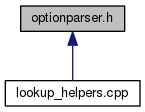
\includegraphics[width=181pt]{optionparser_8h__dep__incl}
\end{center}
\end{figure}
\subsection*{Classes}
\begin{DoxyCompactItemize}
\item 
struct \hyperlink{structoption_1_1Descriptor}{option\+::\+Descriptor}
\begin{DoxyCompactList}\small\item\em Describes an option, its help text (usage) and how it should be parsed. \end{DoxyCompactList}\item 
class \hyperlink{classoption_1_1Option}{option\+::\+Option}
\begin{DoxyCompactList}\small\item\em A parsed option from the command line together with its argument if it has one. \end{DoxyCompactList}\item 
struct \hyperlink{structoption_1_1Arg}{option\+::\+Arg}
\begin{DoxyCompactList}\small\item\em Functions for checking the validity of option arguments. \end{DoxyCompactList}\item 
struct \hyperlink{structoption_1_1Stats}{option\+::\+Stats}
\begin{DoxyCompactList}\small\item\em Determines the minimum lengths of the buffer and options arrays used for \hyperlink{classoption_1_1Parser}{Parser}. \end{DoxyCompactList}\item 
class \hyperlink{classoption_1_1Parser}{option\+::\+Parser}
\begin{DoxyCompactList}\small\item\em Checks argument vectors for validity and parses them into data structures that are easier to work with. \end{DoxyCompactList}\item 
struct \hyperlink{structoption_1_1Parser_1_1Action}{option\+::\+Parser\+::\+Action}
\item 
class \hyperlink{classoption_1_1Stats_1_1CountOptionsAction}{option\+::\+Stats\+::\+Count\+Options\+Action}
\item 
class \hyperlink{classoption_1_1Parser_1_1StoreOptionAction}{option\+::\+Parser\+::\+Store\+Option\+Action}
\item 
struct \hyperlink{structoption_1_1PrintUsageImplementation}{option\+::\+Print\+Usage\+Implementation}
\item 
struct \hyperlink{structoption_1_1PrintUsageImplementation_1_1IStringWriter}{option\+::\+Print\+Usage\+Implementation\+::\+I\+String\+Writer}
\item 
struct \hyperlink{structoption_1_1PrintUsageImplementation_1_1FunctionWriter}{option\+::\+Print\+Usage\+Implementation\+::\+Function\+Writer$<$ Function $>$}
\item 
struct \hyperlink{structoption_1_1PrintUsageImplementation_1_1OStreamWriter}{option\+::\+Print\+Usage\+Implementation\+::\+O\+Stream\+Writer$<$ O\+Stream $>$}
\item 
struct \hyperlink{structoption_1_1PrintUsageImplementation_1_1TemporaryWriter}{option\+::\+Print\+Usage\+Implementation\+::\+Temporary\+Writer$<$ Temporary $>$}
\item 
struct \hyperlink{structoption_1_1PrintUsageImplementation_1_1SyscallWriter}{option\+::\+Print\+Usage\+Implementation\+::\+Syscall\+Writer$<$ Syscall $>$}
\item 
struct \hyperlink{structoption_1_1PrintUsageImplementation_1_1StreamWriter}{option\+::\+Print\+Usage\+Implementation\+::\+Stream\+Writer$<$ Function, Stream $>$}
\item 
class \hyperlink{classoption_1_1PrintUsageImplementation_1_1LinePartIterator}{option\+::\+Print\+Usage\+Implementation\+::\+Line\+Part\+Iterator}
\item 
class \hyperlink{classoption_1_1PrintUsageImplementation_1_1LineWrapper}{option\+::\+Print\+Usage\+Implementation\+::\+Line\+Wrapper}
\end{DoxyCompactItemize}
\subsection*{Namespaces}
\begin{DoxyCompactItemize}
\item 
 \hyperlink{namespaceoption}{option}
\begin{DoxyCompactList}\small\item\em The namespace of The Lean Mean C++ \hyperlink{classoption_1_1Option}{Option} \hyperlink{classoption_1_1Parser}{Parser}. \end{DoxyCompactList}\end{DoxyCompactItemize}
\subsection*{Typedefs}
\begin{DoxyCompactItemize}
\item 
typedef Arg\+Status($\ast$ \hyperlink{namespaceoption_a4cdf403efae65e18bf850e2001b12a2a}{option\+::\+Check\+Arg}) (const Option \&option, bool msg)
\begin{DoxyCompactList}\small\item\em Signature of functions that check if an argument is valid for a certain type of option. \end{DoxyCompactList}\end{DoxyCompactItemize}
\subsection*{Enumerations}
\begin{DoxyCompactItemize}
\item 
enum \hyperlink{namespaceoption_aee8c76a07877335762631491e7a5a1a9}{option\+::\+Arg\+Status} \{ \hyperlink{namespaceoption_aee8c76a07877335762631491e7a5a1a9a353903b042e8eb0aa2f60c0043a58a7e}{option\+::\+A\+R\+G\+\_\+\+N\+O\+NE}, 
\hyperlink{namespaceoption_aee8c76a07877335762631491e7a5a1a9a445e08cb1747e5a22929e7ef2da43b55}{option\+::\+A\+R\+G\+\_\+\+OK}, 
\hyperlink{namespaceoption_aee8c76a07877335762631491e7a5a1a9a83e0837c79c957525918111d33cab3a9}{option\+::\+A\+R\+G\+\_\+\+I\+G\+N\+O\+RE}, 
\hyperlink{namespaceoption_aee8c76a07877335762631491e7a5a1a9a9528e32563b795bd2930b12d0a5e382d}{option\+::\+A\+R\+G\+\_\+\+I\+L\+L\+E\+G\+AL}
 \}\begin{DoxyCompactList}\small\item\em Possible results when checking if an argument is valid for a certain option. \end{DoxyCompactList}
\end{DoxyCompactItemize}
\subsection*{Functions}
\begin{DoxyCompactItemize}
\item 
{\footnotesize template$<$typename O\+Stream $>$ }\\void \hyperlink{namespaceoption_afc8bb7e040a98a0b33ff1ce9da1be0d1}{option\+::print\+Usage} (O\+Stream \&prn, const Descriptor usage\mbox{[}$\,$\mbox{]}, int width=80, int last\+\_\+column\+\_\+min\+\_\+percent=50, int last\+\_\+column\+\_\+own\+\_\+line\+\_\+max\+\_\+percent=75)
\begin{DoxyCompactList}\small\item\em Outputs a nicely formatted usage string with support for multi-\/column formatting and line-\/wrapping. \end{DoxyCompactList}\item 
{\footnotesize template$<$typename Function $>$ }\\void {\bfseries option\+::print\+Usage} (Function $\ast$prn, const Descriptor usage\mbox{[}$\,$\mbox{]}, int width=80, int last\+\_\+column\+\_\+min\+\_\+percent=50, int last\+\_\+column\+\_\+own\+\_\+line\+\_\+max\+\_\+percent=75)\hypertarget{namespaceoption_a846de0735717c8402b76d14f0a7a4430}{}\label{namespaceoption_a846de0735717c8402b76d14f0a7a4430}

\item 
{\footnotesize template$<$typename Temporary $>$ }\\void {\bfseries option\+::print\+Usage} (const Temporary \&prn, const Descriptor usage\mbox{[}$\,$\mbox{]}, int width=80, int last\+\_\+column\+\_\+min\+\_\+percent=50, int last\+\_\+column\+\_\+own\+\_\+line\+\_\+max\+\_\+percent=75)\hypertarget{namespaceoption_a86e12a019c4da81e5031901af9c800cc}{}\label{namespaceoption_a86e12a019c4da81e5031901af9c800cc}

\item 
{\footnotesize template$<$typename Syscall $>$ }\\void {\bfseries option\+::print\+Usage} (Syscall $\ast$prn, int fd, const Descriptor usage\mbox{[}$\,$\mbox{]}, int width=80, int last\+\_\+column\+\_\+min\+\_\+percent=50, int last\+\_\+column\+\_\+own\+\_\+line\+\_\+max\+\_\+percent=75)\hypertarget{namespaceoption_a84764f72d05ba8480143043e3d56ad6a}{}\label{namespaceoption_a84764f72d05ba8480143043e3d56ad6a}

\item 
{\footnotesize template$<$typename Function , typename Stream $>$ }\\void {\bfseries option\+::print\+Usage} (Function $\ast$prn, Stream $\ast$stream, const Descriptor usage\mbox{[}$\,$\mbox{]}, int width=80, int last\+\_\+column\+\_\+min\+\_\+percent=50, int last\+\_\+column\+\_\+own\+\_\+line\+\_\+max\+\_\+percent=75)\hypertarget{namespaceoption_a27bfa29dc37bb1bfc5e0b891509e5881}{}\label{namespaceoption_a27bfa29dc37bb1bfc5e0b891509e5881}

\end{DoxyCompactItemize}


\subsection{Detailed Description}
This is the only file required to use The Lean Mean C++ Option Parser. Just \#include it and you\textquotesingle{}re set. 

The Lean Mean C++ Option Parser handles the program\textquotesingle{}s command line arguments (argc, argv). It supports the short and long option formats of getopt(), getopt\+\_\+long() and getopt\+\_\+long\+\_\+only() but has a more convenient interface. The following features set it apart from other option parsers\+:

\begin{DoxyParagraph}{Highlights\+:}

\begin{DoxyItemize}
\item It is a header-\/only library. Just {\ttfamily \#include \char`\"{}optionparser.\+h\char`\"{}} and you\textquotesingle{}re set. 
\item It is freestanding. There are no dependencies whatsoever, not even the C or C++ standard library. 
\item It has a usage message formatter that supports column alignment and line wrapping. This aids localization because it adapts to translated strings that are shorter or longer (even if they contain Asian wide characters). 
\item Unlike getopt() and derivatives it doesn\textquotesingle{}t force you to loop through options sequentially. Instead you can access options directly like this\+: 
\begin{DoxyItemize}
\item Test for presence of a switch in the argument vector\+: 
\begin{DoxyCode}
\textcolor{keywordflow}{if} ( options[QUIET] ) ... 
\end{DoxyCode}
 
\item Evaluate --enable-\/foo/--disable-\/foo pair where the last one used wins\+: 
\begin{DoxyCode}
\textcolor{keywordflow}{if} ( options[FOO].last()->type() == DISABLE ) ... 
\end{DoxyCode}
 
\item Cumulative option (-\/v verbose, -\/vv more verbose, -\/vvv even more verbose)\+: 
\begin{DoxyCode}
\textcolor{keywordtype}{int} verbosity = options[VERBOSE].\hyperlink{classoption_1_1Option_a8a632dcd89af60fe0806deb756c08f14}{count}(); 
\end{DoxyCode}
 
\item Iterate over all --file=$<$fname$>$ arguments\+: 
\begin{DoxyCode}
\textcolor{keywordflow}{for} (Option* opt = options[FILE]; opt; opt = opt->\hyperlink{classoption_1_1Option_a59ae9aed505f4d410633bb36478a32be}{next}())
 fname = opt->arg; ... 
\end{DoxyCode}
 
\item If you really want to, you can still process all arguments in order\+: 
\begin{DoxyCode}
\textcolor{keywordflow}{for} (\textcolor{keywordtype}{int} i = 0; i < p.optionsCount(); ++i) \{
  Option& opt = buffer[i];
  \textcolor{keywordflow}{switch}(opt.index()) \{
    \textcolor{keywordflow}{case} HELP:    ...
    \textcolor{keywordflow}{case} VERBOSE: ...
    \textcolor{keywordflow}{case} FILE:    fname = opt.arg; ...
    \textcolor{keywordflow}{case} UNKNOWN: ...
\end{DoxyCode}
 
\end{DoxyItemize}
\end{DoxyItemize}~\newline
Despite these features the code size remains tiny. It is smaller than \href{http://uclibc.org}{\tt u\+Clibc}\textquotesingle{}s G\+NU getopt() and just a couple 100 bytes larger than u\+Clibc\textquotesingle{}s S\+U\+Sv3 getopt(). ~\newline
(This does not include the usage formatter, of course. But you don\textquotesingle{}t have to use that.)
\end{DoxyParagraph}
\begin{DoxyParagraph}{Download\+:}
Tarball with examples and test programs\+: \href{http://sourceforge.net/projects/optionparser/files/optionparser-1.4.tar.gz/download}{\tt optionparser-\/1.\+4.\+tar.\+gz} ~\newline
Just the header (this is all you really need)\+: \href{http://optionparser.sourceforge.net/optionparser.h}{\tt optionparser.\+h}
\end{DoxyParagraph}
\begin{DoxyParagraph}{Changelog\+:}
{\bfseries Version 1.\+4\+:} Fixed 2 print\+Usage() bugs that messed up output with small C\+O\+L\+U\+M\+NS values ~\newline
{\bfseries Version 1.\+3\+:} Compatible with Microsoft Visual C++. ~\newline
{\bfseries Version 1.\+2\+:} Added \hyperlink{classoption_1_1Option_a3aa2957b19ad5815873441b415d56050}{Option\+:\+:namelen} and removed the extraction of short option characters into a special buffer. ~\newline
 Changed \hyperlink{structoption_1_1Arg_aadb5316ecbc9eb0a7f0019d14bf35ad0}{Arg\+:\+:Optional} to accept arguments if they are attached rather than separate. This is what G\+NU getopt() does and how P\+O\+S\+IX recommends utilities should interpret their arguments.~\newline
{\bfseries Version 1.\+1\+:} Optional mode with argument reordering as done by G\+NU getopt(), so that options and non-\/options can be mixed. See \hyperlink{classoption_1_1Parser_a6e0b5778d1cfbd6cd51240e74d01e138}{Parser\+:\+:parse()}.
\end{DoxyParagraph}
\begin{DoxyParagraph}{Feedback\+:}
Send questions, bug reports, feature requests etc. to\+: {\ttfamily {\bfseries optionparser-\/feedback~(a)~lists.\+sourceforge.\+net}} 
\end{DoxyParagraph}
\begin{DoxyParagraph}{Example program\+:}
(Note\+: {\ttfamily option\+:}\+:$\ast$ identifiers are links that take you to their documentation.) 
\begin{DoxyCode}
\textcolor{preprocessor}{#error EXAMPLE SHORTENED FOR READABILITY. BETTER EXAMPLES ARE IN THE .TAR.GZ!}
\textcolor{preprocessor}{#include <iostream>}
\textcolor{preprocessor}{#include "\hyperlink{optionparser_8h}{optionparser.h}"}

\textcolor{keyword}{enum}  optionIndex \{ UNKNOWN, HELP, PLUS \};
\textcolor{keyword}{const} \hyperlink{structoption_1_1Descriptor}{option::Descriptor} usage[] =
\{
 \{UNKNOWN, 0,\textcolor{stringliteral}{""} , \textcolor{stringliteral}{""}    ,\hyperlink{structoption_1_1Arg_a7fc01987899c91c6b6a1be5711a46e22}{option::Arg::None}, \textcolor{stringliteral}{"USAGE: example [options]\(\backslash\)n\(\backslash\)n"}
                                            \textcolor{stringliteral}{"Options:"} \},
 \{HELP,    0,\textcolor{stringliteral}{""} , \textcolor{stringliteral}{"help"},\hyperlink{structoption_1_1Arg_a7fc01987899c91c6b6a1be5711a46e22}{option::Arg::None}, \textcolor{stringliteral}{"  --help  \(\backslash\)tPrint usage and exit."} \},
 \{PLUS,    0,\textcolor{stringliteral}{"p"}, \textcolor{stringliteral}{"plus"},\hyperlink{structoption_1_1Arg_a7fc01987899c91c6b6a1be5711a46e22}{option::Arg::None}, \textcolor{stringliteral}{"  --plus, -p  \(\backslash\)tIncrement count."} \},
 \{UNKNOWN, 0,\textcolor{stringliteral}{""} ,  \textcolor{stringliteral}{""}   ,\hyperlink{structoption_1_1Arg_a7fc01987899c91c6b6a1be5711a46e22}{option::Arg::None}, \textcolor{stringliteral}{"\(\backslash\)nExamples:\(\backslash\)n"}
                                            \textcolor{stringliteral}{"  example --unknown -- --this\_is\_no\_option\(\backslash\)n"}
                                            \textcolor{stringliteral}{"  example -unk --plus -ppp file1 file2\(\backslash\)n"} \},
 \{0,0,0,0,0,0\}
\};

\textcolor{keywordtype}{int} main(\textcolor{keywordtype}{int} argc, \textcolor{keywordtype}{char}* argv[])
\{
  argc-=(argc>0); argv+=(argc>0); \textcolor{comment}{// skip program name argv[0] if present}
  \hyperlink{structoption_1_1Stats}{option::Stats}  stats(usage, argc, argv);
  \hyperlink{classoption_1_1Option}{option::Option} options[stats.options\_max], buffer[stats.buffer\_max];
  \hyperlink{classoption_1_1Parser}{option::Parser} parse(usage, argc, argv, options, buffer);

  \textcolor{keywordflow}{if} (parse.error())
    \textcolor{keywordflow}{return} 1;

  \textcolor{keywordflow}{if} (options[HELP] || argc == 0) \{
    \hyperlink{namespaceoption_afc8bb7e040a98a0b33ff1ce9da1be0d1}{option::printUsage}(std::cout, usage);
    \textcolor{keywordflow}{return} 0;
  \}

  std::cout << \textcolor{stringliteral}{"--plus count: "} <<
    options[PLUS].\hyperlink{classoption_1_1Option_a8a632dcd89af60fe0806deb756c08f14}{count}() << \textcolor{stringliteral}{"\(\backslash\)n"};

  \textcolor{keywordflow}{for} (\hyperlink{classoption_1_1Option}{option::Option}* opt = options[UNKNOWN]; opt; opt = opt->
      \hyperlink{classoption_1_1Option_a59ae9aed505f4d410633bb36478a32be}{next}())
    std::cout << \textcolor{stringliteral}{"Unknown option: "} << opt->name << \textcolor{stringliteral}{"\(\backslash\)n"};

  for (\textcolor{keywordtype}{int} i = 0; i < parse.nonOptionsCount(); ++i)
    std::cout << \textcolor{stringliteral}{"Non-option #"} << i << \textcolor{stringliteral}{": "} << parse.nonOption(i) << \textcolor{stringliteral}{"\(\backslash\)n"};
\}
\end{DoxyCode}

\end{DoxyParagraph}
\begin{DoxyParagraph}{Option syntax\+:}
\begin{DoxyItemize}
\item The Lean Mean C++ Option Parser follows P\+O\+S\+IX {\ttfamily getopt()} conventions and supports G\+N\+U-\/style {\ttfamily getopt\+\_\+long()} long options as well as Perl-\/style single-\/minus long options ({\ttfamily getopt\+\_\+long\+\_\+only()}). \item short options have the format {\ttfamily -\/X} where {\ttfamily X} is any character that fits in a char. \item short options can be grouped, i.\+e. {\ttfamily -\/X -\/Y} is equivalent to {\ttfamily -\/\+XY}. \item a short option may take an argument either separate ({\ttfamily -\/X foo}) or attached ({\ttfamily -\/\+Xfoo}). You can make the parser accept the additional format {\ttfamily -\/X=foo} by registering {\ttfamily X} as a long option (in addition to being a short option) and enabling single-\/minus long options. \item an argument-\/taking short option may be grouped if it is the last in the group, e.\+g. {\ttfamily -\/\+A\+B\+C\+Xfoo} or {\ttfamily  -\/\+A\+B\+CX foo } ({\ttfamily foo} is the argument to the {\ttfamily -\/X} option). \item a lone minus character {\ttfamily \textquotesingle{}-\/\textquotesingle{}} is not treated as an option. It is customarily used where a file name is expected to refer to stdin or stdout. \item long options have the format {\ttfamily --option-\/name}. \item the option-\/name of a long option can be anything and include any characters. Even {\ttfamily =} characters will work, but don\textquotesingle{}t do that. \item \mbox{[}optional\mbox{]} long options may be abbreviated as long as the abbreviation is unambiguous. You can set a minimum length for abbreviations. \item \mbox{[}optional\mbox{]} long options may begin with a single minus. The double minus form is always accepted, too. \item a long option may take an argument either separate ({\ttfamily  --option arg }) or attached ({\ttfamily  --option=arg }). In the attached form the equals sign is mandatory. \item an empty string can be passed as an attached long option argument\+: {\ttfamily  --option-\/name= }. Note the distinction between an empty string as argument and no argument at all. \item an empty string is permitted as separate argument to both long and short options. \item Arguments to both short and long options may start with a {\ttfamily \textquotesingle{}-\/\textquotesingle{}} character. E.\+g. {\ttfamily  -\/\+X-\/X }, {\ttfamily -\/X -\/X} or {\ttfamily  --long-\/X=-\/X }. If {\ttfamily -\/X} and {\ttfamily --long-\/X} take an argument, that argument will be {\ttfamily \char`\"{}-\/\+X\char`\"{}} in all 3 cases. \item If using the built-\/in \hyperlink{structoption_1_1Arg_aadb5316ecbc9eb0a7f0019d14bf35ad0}{Arg\+:\+:Optional}, optional arguments must be attached. \item the special option {\ttfamily --} (i.\+e. without a name) terminates the list of options. Everything that follows is a non-\/option argument, even if it starts with a {\ttfamily \textquotesingle{}-\/\textquotesingle{}} character. The {\ttfamily --} itself will not appear in the parse results. \item the first argument that doesn\textquotesingle{}t start with {\ttfamily \textquotesingle{}-\/\textquotesingle{}} or {\ttfamily \textquotesingle{}--\textquotesingle{}} and does not belong to a preceding argument-\/taking option, will terminate the option list and is the first non-\/option argument. All following command line arguments are treated as non-\/option arguments, even if they start with {\ttfamily \textquotesingle{}-\/\textquotesingle{}} . ~\newline
 N\+O\+TE\+: This behaviour is mandated by P\+O\+S\+IX, but G\+NU getopt() only honours this if it is explicitly requested (e.\+g. by setting P\+O\+S\+I\+X\+L\+Y\+\_\+\+C\+O\+R\+R\+E\+CT). ~\newline
 You can enable the G\+NU behaviour by passing {\ttfamily true} as first argument to e.\+g. \hyperlink{classoption_1_1Parser_a6e0b5778d1cfbd6cd51240e74d01e138}{Parser\+:\+:parse()}. \item Arguments that look like options (i.\+e. {\ttfamily \textquotesingle{}-\/\textquotesingle{}} followed by at least 1 character) but aren\textquotesingle{}t, are N\+OT treated as non-\/option arguments. They are treated as unknown options and are collected into a list of unknown options for error reporting. ~\newline
 This means that in order to pass a first non-\/option argument beginning with the minus character it is required to use the {\ttfamily --} special option, e.\+g. 
\begin{DoxyCode}
program -x -- --strange-filename
\end{DoxyCode}
 In this example, {\ttfamily --strange-\/filename} is a non-\/option argument. If the {\ttfamily --} were omitted, it would be treated as an unknown option. ~\newline
 See \hyperlink{structoption_1_1Descriptor_a470c449dfa894c9bfda2dae026142b4b}{option\+::\+Descriptor\+::longopt} for information on how to collect unknown options. \end{DoxyItemize}

\end{DoxyParagraph}

\chapter{Example Documentation}
\hypertarget{command_control_strategy_group_example_8cpp-example}{}\section{command\+\_\+control\+\_\+strategy\+\_\+group\+\_\+example.\+cpp}

\begin{DoxyCodeInclude}
\end{DoxyCodeInclude}
 
\hypertarget{command_group_example_8cpp-example}{}\section{command\+\_\+group\+\_\+example.\+cpp}

\begin{DoxyCodeInclude}
\end{DoxyCodeInclude}
 
\hypertarget{command_module_example_8cpp-example}{}\section{command\+\_\+module\+\_\+example.\+cpp}

\begin{DoxyCodeInclude}
\end{DoxyCodeInclude}
 
\hypertarget{command_settings_group_example_8cpp-example}{}\section{command\+\_\+settings\+\_\+group\+\_\+example.\+cpp}

\begin{DoxyCodeInclude}
\end{DoxyCodeInclude}
 
\hypertarget{command_spring_constants_group_example_8cpp-example}{}\section{command\+\_\+spring\+\_\+constants\+\_\+group\+\_\+example.\+cpp}

\begin{DoxyCodeInclude}
\end{DoxyCodeInclude}
 
\hypertarget{feedback_async_group_example_8cpp-example}{}\section{feedback\+\_\+async\+\_\+group\+\_\+example.\+cpp}

\begin{DoxyCodeInclude}
\end{DoxyCodeInclude}
 
\hypertarget{feedback_sync_group_example_8cpp-example}{}\section{feedback\+\_\+sync\+\_\+group\+\_\+example.\+cpp}

\begin{DoxyCodeInclude}
\end{DoxyCodeInclude}
 
\hypertarget{feedback_sync_module_example_8cpp-example}{}\section{feedback\+\_\+sync\+\_\+module\+\_\+example.\+cpp}

\begin{DoxyCodeInclude}
\end{DoxyCodeInclude}
 
\hypertarget{info_sync_group_example_8cpp-example}{}\section{info\+\_\+sync\+\_\+group\+\_\+example.\+cpp}

\begin{DoxyCodeInclude}
\end{DoxyCodeInclude}
 
\hypertarget{lookup_group_example_8cpp-example}{}\section{lookup\+\_\+group\+\_\+example.\+cpp}
How to lookup a group -\/ simple.


\begin{DoxyCodeInclude}
\end{DoxyCodeInclude}
 
\hypertarget{lookup_group_general_example_8cpp-example}{}\section{lookup\+\_\+group\+\_\+general\+\_\+example.\+cpp}
How to lookup a group -\/ generalized using command line arguments.


\begin{DoxyCodeInclude}
\end{DoxyCodeInclude}
 
\hypertarget{lookup_helpers_8cpp-example}{}\section{lookup\+\_\+helpers.\+cpp}
File with parsing of command line arguments and actual group generation used by general examples above.


\begin{DoxyCodeInclude}
\end{DoxyCodeInclude}
 
\hypertarget{lookup_module_example_8cpp-example}{}\section{lookup\+\_\+module\+\_\+example.\+cpp}
How to lookup a module -\/ simple.


\begin{DoxyCodeInclude}
\end{DoxyCodeInclude}
 
\hypertarget{lookup_module_general_example_8cpp-example}{}\section{lookup\+\_\+module\+\_\+general\+\_\+example.\+cpp}
How to lookup a module -\/ generalized using command line arguments.


\begin{DoxyCodeInclude}
\end{DoxyCodeInclude}
 
\hypertarget{master_slave_async_group_example_8cpp-example}{}\section{master\+\_\+slave\+\_\+async\+\_\+group\+\_\+example.\+cpp}

\begin{DoxyCodeInclude}
\end{DoxyCodeInclude}
 
\hypertarget{master_slave_group_example_8cpp-example}{}\section{master\+\_\+slave\+\_\+group\+\_\+example.\+cpp}

\begin{DoxyCodeInclude}
\end{DoxyCodeInclude}
 
%--- End generated contents ---

% Index
\backmatter
\newpage
\phantomsection
\clearemptydoublepage
\addcontentsline{toc}{chapter}{Index}
\printindex

\end{document}
